  \documentclass[11pt,titlepage,a5paper]{book}



%\usepackage[T2A, T1]{fontenc} 
%\usepackage[russian, ngerman]{babel}

  \usepackage[T1]{fontenc}  
  \usepackage[ngerman]{babel}
 

 
  \usepackage[utf8]{inputenc}
 


 \usepackage{graphicx}
 \usepackage{geometry}
 \usepackage{pstricks}

%Musiknoten 
 \usepackage{wasysym}
 
 
% \usepackage[style=numeric-comp,backend=bibtex]{biblatex}
% \addbibresource{Bilbliothek.bib}
 
 \pagestyle{plain}

\clubpenalty3000
\widowpenalty3000
\displaywidowpenalty=3000
 
%\frenchspacing 

\parindent0em 
\setlength{\parskip}{0.4ex plus 0.6ex minus 0.4ex}
\sloppy

\geometry{left=2.5cm,right=2cm,bottom=3.5cm,top=2.0cm}

 \author{von\\[0.8ex]Felicitas Stotz}
 \title{\bf\Huge Die Horussöhne}
 
 \newcommand{\sterne}{\par{\centering ***\par}}
 %\newcommand{\ti}{"`}
 %\newcommand{\ho}{"'}

% \newenvironment{tg}{\begin{quote}\em}{\end{quote}}

 \newcommand{\am}{Amélie }
  
 \newenvironment{dichter}{\begin{flushright}}{\end{flushright}}

\newcommand{\changefont}[3]{
\fontfamily{#1} \fontseries{#2} \fontshape{#3} \selectfont}



 \begin{document}
% .
% \newpage
% \newpage
 
 \changefont{ppl}{m}{n}
 
  %\maketitle
   
 \begin{titlepage} 

%\includegraphics[width=0.9\textwidth]{/home/felicitas/133_1.JPG}

\begin{pspicture}
(-4.9,8.5)
\rput(0cm,0cm){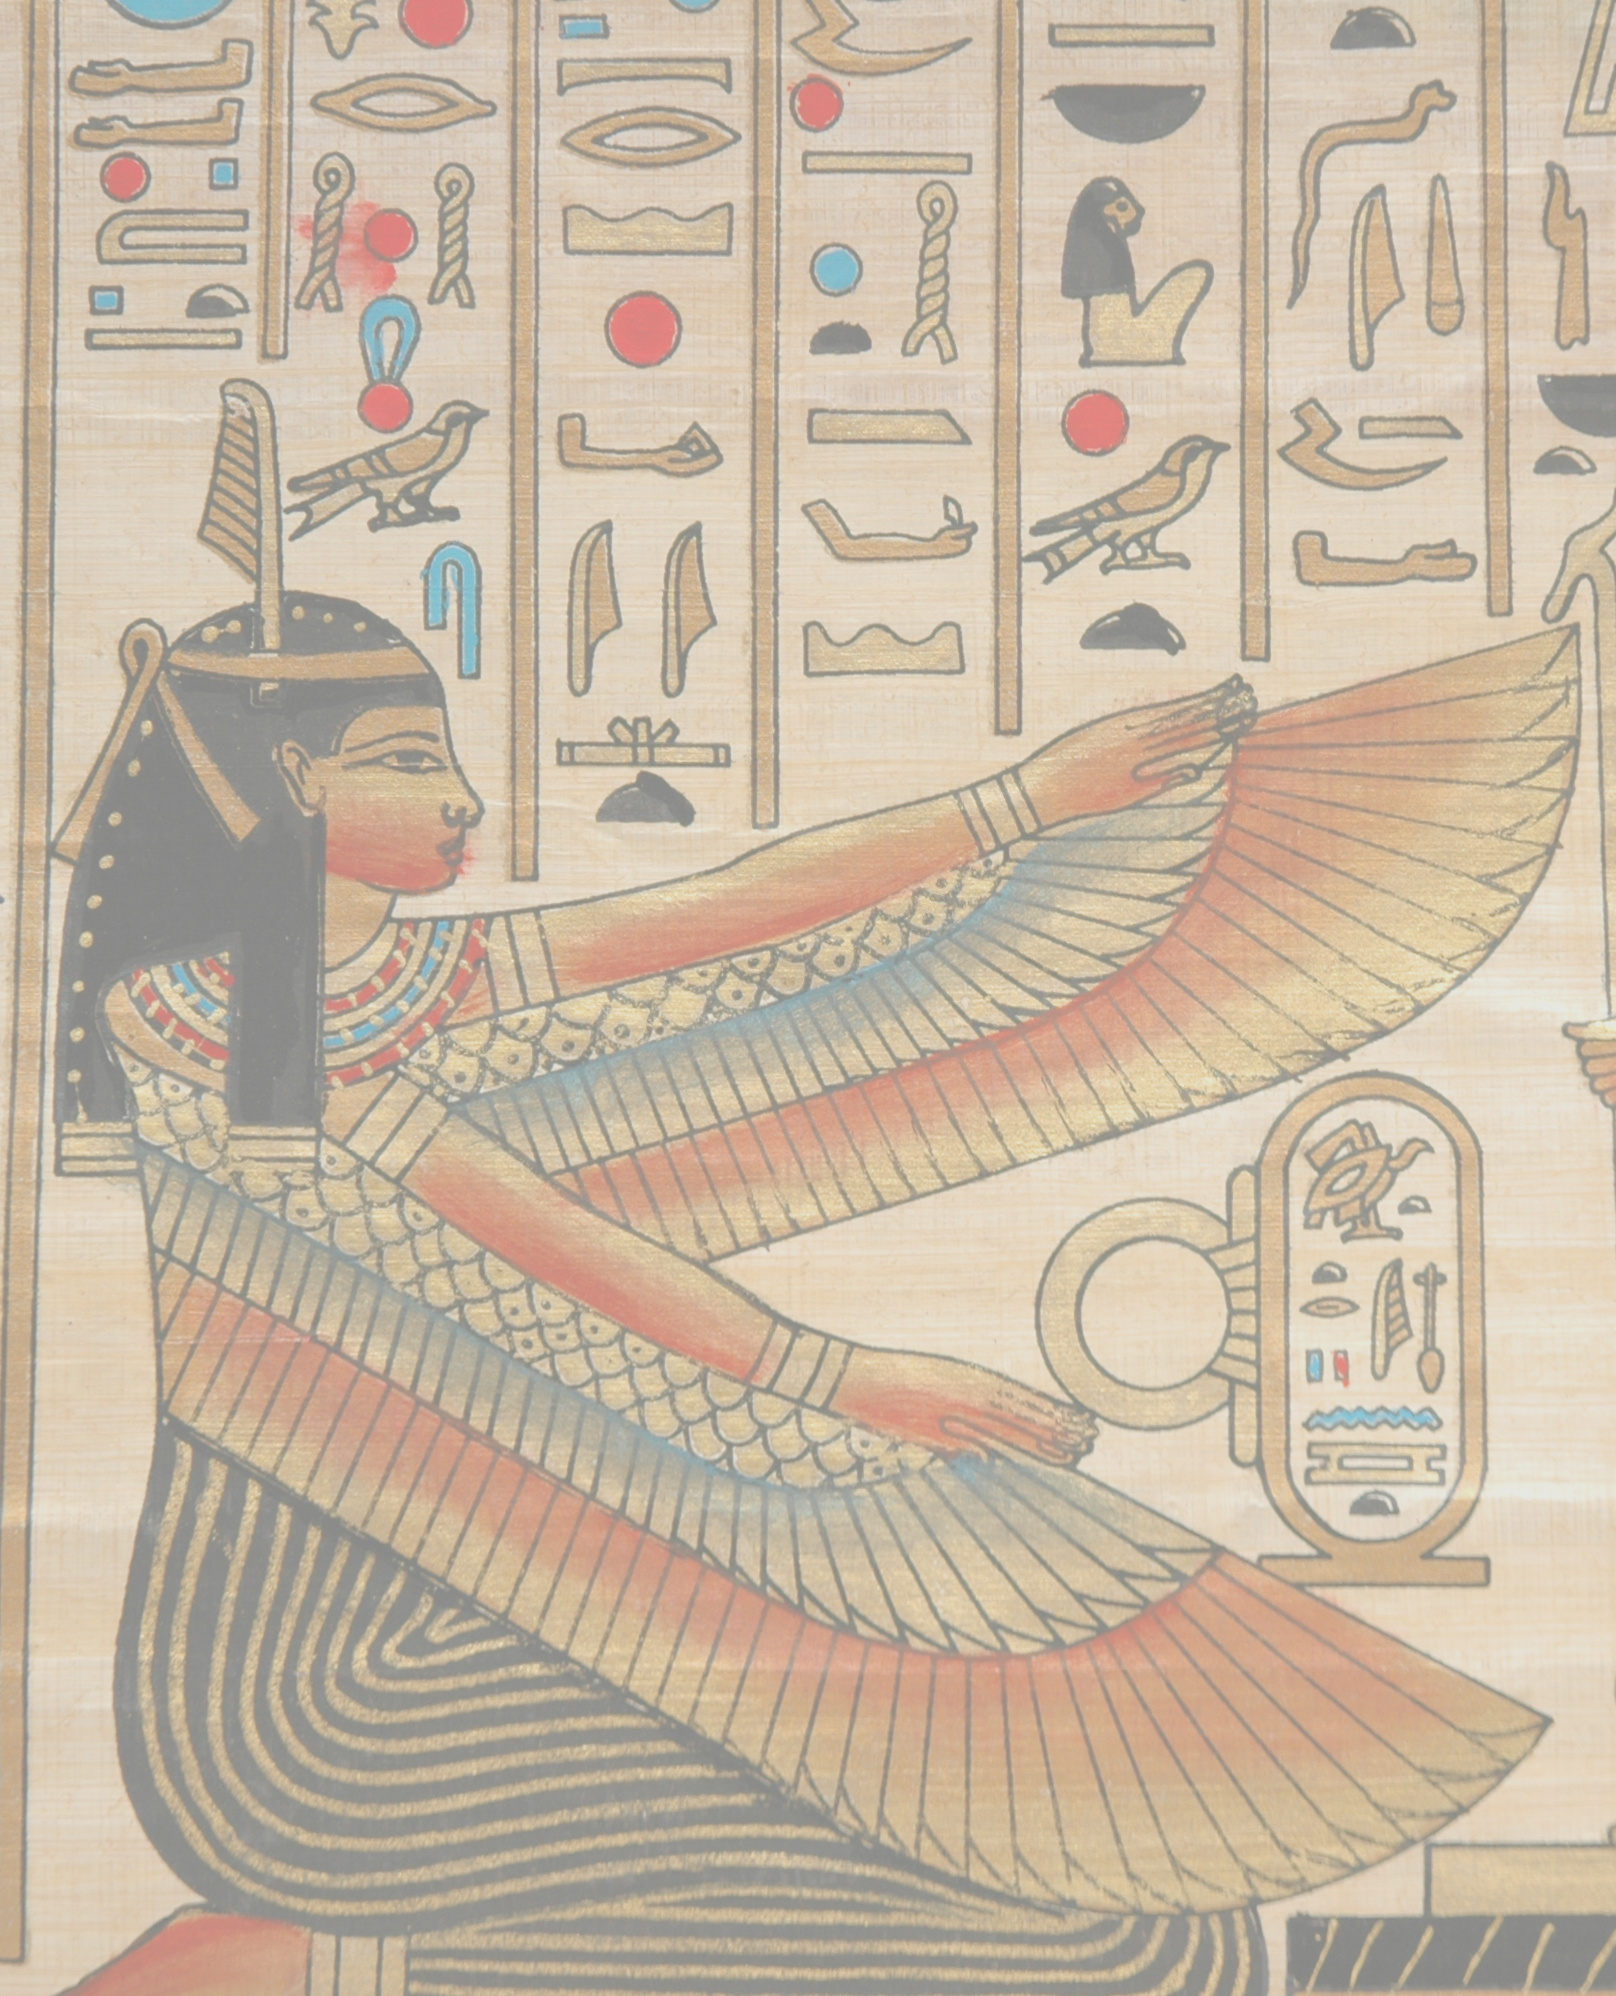
\includegraphics[width=\paperwidth,height=\paperheight]{Titel-Hell}}
\end{pspicture}
  
  \vspace*{-0.4\textheight}
  {\fontsize{40}{60}\selectfont Die Horussöhne}\\[38ex]
  {\huge Felicitas Stotz}\\[8ex]
   \today
 
 \end{titlepage}


\thispagestyle{empty}


\chapter*{}

\section*{Titelei}

%\begin{tg}
\begin{verse}



Die Schrift des Verborgenen Raumes.\\
Die Standorte der Bau und der Götter,\\
die Schatten und Achu, und was getan wird.

Der Anfang ist das Horn des Westens,\\
das Tor des Westhorizontes;\\
das Ende ist die Urfinsternis,\\
das Tor des Westhorizontes.

Zu kennen die Unterweltlichen Bau,\\
zu kennen die Geheimen Bau,\\
zu kennen die Tore\\
und die Wege, auf denen der Grösste Gott wandelt.

Zu kennen, was getan wird, \\
zu kennen, was in den Stunden ist, und ihre Götter, \\
zu kennen den Lauf der Stunden, und ihre Götter.


Zu kennen ihre Verklärungen des RE,\\
zu kennen, was er ihnen zuruft,\\
zu kennen die Gedeihenden und die Ver\-nich\-te\-ten.{}\\

\end{verse}
%\end{tg}



\chapter*{2. Februar (Prolog)}
\addcontentsline{toc}{chapter}{Prolog: 2 . Februar (Prolog)}

Die Wahrheit ist: Wir wissen es nicht! 

Was wir wissen, sind die Dinge, die wir wahr-nehmen. Wir nehmen sie mit unseren Sinnen auf und bewerten sie. Dabei bewerten wir sie nach nützlich oder unnütz, essbar oder nicht essbar und kommt es für die Paarung in Frage? Wenn wir die Dinge als wahr bezeichnen, die wir mit den Sinnen in der physischen Welt erfahren, sind wir auf der sichereren Seite. Nicht ganz sicher, aber immerhin\dots

Dann gibt es unser Gehirn, unsere Emotionen, unsere Träume, unsere Hoffnungen und Wünsche, unsere Ängste, unseren Glauben\dots Sie sind unsichtbar, unfassbar, aber denkbar. Das ist interessant, weil wir in unserem Gehirn die sichtbaren Wahrnehmungen und die unsichtbaren Gedanken miteinander untrennbar vermischen. Und weil wir sie vermischen, wissen wir schliesslich nicht mehr, was wir wahrnehmen könnten und was denken. Wissen wir nicht, was wir erfahren haben, was wir kennen und was wir nicht wissen können, weil wir es mit einem grauen, weichen Fleischklops gedacht haben.

Wir neigen dazu, uns für alles eine Antwort zu basteln. Denn eine erklärbare Welt ist eine überschaubare Welt. Eine Welt, in der man weiss, wo der Tiger wohnt\dots \footnote{Eine beliebte Tiger-Adresse ist der indische Dschungel und Sibirien.} Dann kommen wir mit den Unsichtbarkeiten unseres Daseins besser zurecht. Den dunklen Gedanken in der Nacht, wenn wir nicht mehr sicher sind, ob wir wissen, wo der Tiger wohnt.

Und wenn wir die samtweichen Tigerpranken an unserem Schlafpelz vorbei schleichen hören, wünschen wir uns jemanden, der uns beschützt. Einen Krieger! Zwei starke Krieger! Zwanzig starke Krieger!

 Viele, starke Riesenkrieger, die dem Tiger in den Hinter treten und ihn im hohen Bogen bis nach Sibirien schicken, damit wir genau wissen, wo er wohnt und sich seinen  verd***ten, schmerzenden, kalten Hintern schleckt! Weit weg im verd***t Sibirien!
 
Vielleicht, -wir wissen es nicht. Vielleicht sind so die ersten Götter entstanden? => Götter = Tigerschnelllieferservice für die Russen! 

Und wenn wir beginnen unser Gehirn für Erklärungen der Dinge zu bemühen, die wir nicht verstehen, dann könnten wir auf die Idee kommen, der Tigerschnelllieferservice könnte viel mehr.

Vielleicht würden wir die Chance ergreifen und uns vorstellen, dass die starken Riesenkrieger die Welt erschaffen haben. Und wenn sie zusammen schaffen, dann brauchen sie einen Chef! Und wo wohnt der Chef der starken Riesenkrieger, während seine Jungs die Welt bauen? Logisch, auf der Sonne! Die ist ein würdiger Chefsessel! Und wo starke Jungs sind und ein Chef, da dürfen auch die Frauen und Mütter nicht fehlen\dots 

Et voila! Fertig ist die Götterwelt! Gibt es sie, gibt es sie nicht? Wir wissen es nicht. Was wir jedoch wissen und kennen, ist die Sehnsucht die Dinge zu verstehen, die Fäden der Geschichte zu finden, damit wir etwas haben, an dem wir unseren Sinn finden und ihm folgen können. Götter können dafür ein nützliches Konzept bereit halten. Eine gute Erklärung, wieso es die Welt gibt und eine, die die Verantwortlichkeiten klärt.

=> Götter = Weltenerbauer => Verantwortlich = Praktisch\footnote{Sich im Geiste Dinge vorzustellen um Informationen zu bekommen, ist völlig okay. Schliesslich haben wir diese tolle Denkkiste in unserem Kopf. Schwierigkeiten bekommen wir dann, wenn wir uns von unserem exzentrischen Denkkasten Unsichtbarkeiten als Dogmen verkaufen lassen! Also, wenn ein kleiner, grüner Zwerg Dir sagt, was Du tun sollst, dann hör nicht auf ihn. Wenn er Dir jedoch interessante Informationen zukommen lässt, dann brauche sie bei Deiner Entscheidungssuche. Allerdings erst, wenn Du darüber nachgedacht hast.}

Götter sind kreativ und eine ihre beliebtesten Hauptaufgaben ist die Schöpfung. Es gibt viele verschiedene Versionen und Ideen bei den Menschen, wie die Erde in den Zustand gekommen ist, in dem sie sich zur Zeit befindet. Und viele Jahrtausende waren sich unsere Vorfahren einig, es sind Götter gewesen. Einer, viele, egal, aber Götter. Unsichtbare, dem Menschen überlegene Wesen, die alles mehr oder weniger leiteten und im Griff hatten.

Heute, nur am Rande bemerkt, lachen die Menschen über dieses Konzept. Sie glauben nicht an Götter, sondern an die Wissenschaft, was bedeutet, alles hat sich entwickelt. Wie genau das gegangen ist, ist so kompliziert, das verstehen nur wenige. (Früher nannte man die Wenigen mit dem "`geheimen Wissen"' "`Eingeweihte"' und dieses Wissen wurde eifersüchtig von ihnen gehütet, aber das war früher. Ha! Hahaha! Heute nennt man es Lizenzrecht.) 

Wenn wir verschiedene Schöpfungsgeschichten anschauen, werden wir feststellen, Götter sind nicht nett. Und in diesem Sinne, liegt auch in unserer Zeit die Frage nahe, ob der Mensch nicht doch göttlichen Ursprunges ist.\footnote{Das liegt näher, als die Vermutung, einiger heutiger "`Eingeweihter"', die glauben, der Mensch sei ein Affe. Aber die Affen können nichts für den Zustand der Erde und es ist gemein, sie ungefragt in die Sache mit der Erde und den menschlichen Zerstörungsversuchen mit hinein zu ziehen. Das haben sie nicht verdient, für ihre Ähnlichkeit mit den Menschen können sie schliesslich nichts.}

\sterne

Unsere Geschichte einer göttlichen Reisegruppe beginnt an einer Stelle der Schöpfung, als die Menschheit sich an einem ähnlichen Punkt befand wie wir heute, wenn wir alten Überlieferungen glauben. Natürlich war dennoch alles anders\dots

Nebelverhangen war das Land Atlantis. Die Menschen besassen weder einen Körper, wie wir ihn kennen, noch hatten sie unser heutiges Bewusstsein. Die Menschen, sie träumten, auch wenn sie wach waren. Dabei waren die Atlantier hoch begabt: Sie waren hellsichtig und konnten die Kräfte, die in den Pflanzen und Steinen vorhanden waren auf diese Weise nutzten.  Sie flogen in Fahrzeugen herum, die mit der Kraft ihrer Gedanken und Kristallen angetrieben waren.

Während wir uns dies schwer vorstellen können, hätten die Atlantier vielleicht unsere Form der Fortbewegung überraschen gefunden: Wir nutzen die Kräfte der Natur, dank unserer weit entwickelten Fähigkeit zu denken. Damit haben wir ein Gefährt entwickelt, das aus Metall gebaut ist und mit Pflanzenkraft angetrieben wird, das Auto.

Was die Atlantier jedoch am meisten von uns heute unterschied, ist nicht ihr merkwürdiger zu Beginn dieser Zeit knochenloser Körper und ihre Hellsichtigkeit, die ihnen ein ähnlich komfortables, weitentwickeltes Leben bescherte. Nein, der grösste Unterschied war, sie kannten ihre Götter! Persönlich. Mit Vor- und Nachnamen und Adresse! Was nicht viel half, denn wie wir wissen, ging Atlantis kläglich unter.

Einer, der nicht unterging, so sagt es die Legende, weil er weise war und sich deshalb dem Wohlwollen der atlantischen Götter erfreute, war Thot. Thot konnte vor dem Untergang von Atlantis flüchten. Und der damals sehr begabte, aber menschliche Thot floh nach Ägypten und fand dort für sich und sein geheimes, atlantisches Wissen eine neue Heimat.

Thot wurde später selbst Gott im Ägypten und war auch bei den Griechen kein unbekannter. Im Gegenteil, sie nannten ihn, wiederum nach ihrem Gott Hermes: Hermes Trismegistos. Thot war ein Tüftler, Erfinder und Philosoph. Dabei ist er nicht der mächtigste der ägyptischen Götter\dots


Er ist allerdings der Gott, der sich am besten als Reiseleiter eignet, weil er selbst als Mensch seine Karriere begonnen hat. Für eine Reisegruppe von Göttern, die teilweise nicht über menschliche Körper verfügen, oder nie aus dem Jenseits, das in Ägypten Duat heisst, heraus gekommen sind, ist es von Vorteil einen gut informierten Reiseleiter zu haben.

Der Jenseitsbereich ist um die Erde herum, ein riesiger Raum für alle Götter, die für die Erde zuständig sind und die Verstorbenen. Allerdings haben die Götter des einen Zeitalters, des einen oder anderen Landes ihre ganz spezifischen Aufgaben. Nicht alle Götter kümmern sich um alles. Andere haben sich auf den "`Altenteil"' zurückgezogen und geben den jüngeren Göttern Tipps, wie man tüchtige Blitze schleudern kann, ohne dabei die ganze Gemeinde auszulöschen. Im Laufe der Zeit hat sich dieser Bereich genauso weiterentwickelt wie die Erde und Menschen.

Wenn Menschen jedoch einen unbestechlichen Wächtergott auf grausame Weise hintergehen, seinen Schutzbefohlenen schaden und damit seine Unbestechlickeit ins Wanken bringen, wenn ein Gott, der in Rente gegangen ist, leiden muss, weil er seiner Zeit voraus war, und er jetzt die Chance der Heilung hat und wenn eine uralte Göttin nicht einmal als Hausmädchen getarnt, ihre geheimen Initiationen durchführen kann, weil plötzlich ein Fluch auftaucht, dann können auch alte Götter sich für eine Reise entschliessen und internationale zusammenarbeiten..

Und so kommt es, dass der grosse Hermes Trismegistos, der "`dreimal grosse Hermes"' genannte Thot, in einer kalten, nebeligen Nacht nach Basel kommt. Er war verabredet und wollte gleichzeitig eine Unterkunft für seine Reisegruppe in Augenschein nehmen.

Thot kannte seine Pappenheimer an jedem Ort. Ihm blieb kein Ort an dem hermetische Künste eine Rolle spielten unbekannt. In Basel einen Wohnort für sein buntes Reisegrüppchen zu finden war einfach. Was liegt näher als die Damen und Herren an dem Ort unterzubringen, an dem ein ehemaliger Adept der Alchemie und Hermetik seinen grossen Auftritt hatte: der grosse Cagliostro? Für die einen ein Scharlatan und für die anderen ein Grossmeister der ägyptischen Logen und Besitzer des Steines der Weisen. Als Thot am Rheinsprung vor den zwei grossen Häusern der Gebrüder Sarasin stand, nickte er zufrieden. Schliesslich wollen auch die abenteuerlustigsten Götter und vor allem Göttinnen nicht auf einen Hauch an Luxus verzichten.

Im berühmten Oktagon, dem achteckigen Zimmer des weissen Hauses des ehrwürdigen Jakob Sarasin, trifft sich der alte ägyptische Gott mit seinen nordischen Freunden Berta, auch bekannt als Frau Holle und Hans, dem "`Wilde Maa"'.

Während Thot sich in einen Ohrensessel gesetzt hatte, von denen zwei im Raum standen, lief Berta im Raum auf und ab. Sie steckte in einem langen schwarzen Kleid und einer weissen Schürze. Sie sah aus wie ein altes, verhutzeltes Hausmädchen. In ihren grauen, kurzen Locken steckt ein weisses Häubchen. Ab und zu schauten ihre Füsse, die in derben, braunen, orthopädischen Schuhen stecken unter dem Kleid hervor. Vor der Tür im Gang stand ein Reisigbesen. Ab und zu nahm sie einen Schluck aus dem Kristallglas, das mit einem rauchig duftenden, bernsteinfarbenem Whisky gefüllt war. Es stand auf einem kleinen runden Nussholztischchen.

Ein zartes Grunzen ertönte. Von dem zierlichen, mit Seide bezogenem Sofa, schauten nur die geschwungenen, dünnen Beinchen hervor, der Rest war unter  dem wilden Mann begraben. Ausser einem Schurz aus Laub, Fell und Zweigen und einer Krone aus Eichenlaub war er nackt. Seine Haut schimmerte goldbraun und unter der Haut zeichneten sich die kräftigen Muskeln ab. Das Gesicht war faltig und die wilden Locken schimmerten nicht nur braun und rot, sondern grün. Da das Sofa viel zu klein war, hing ein Bein über die Lehne und das andere ragte weit ins Zimmer. Eine Hand lag auf den Boden und wenn der Wilde Mann schnarchte, zitterten die Blätter seiner Krone hingebungsvoll. Vor dem Sofa lag ein Dackel. Er hatte sich lang ausgestreckt und sah aus wie eine Pelzwurst mit vier kurzen Beinen und einer schwarzen Nase. Der Dackel schnarchte mit seinem Herrchen in bachscher Fugenmanier. Draussen hörten Berta und Thot einige Krähen von den Dächern krächzen.
 
"`Interessant, äusserst interessant!"' Thot legte die schlanken Fingerspitzen aneinander. Er bevorzugte einen zeitgenössischen, schlichten, schwarzen Anzug. Sein Hemd war weiss-grau gestreift und er trug eine hellgraue Krawatte. In einer angesehenen Anwaltskanzlei wäre er heutigen Tages vermutlich nicht aufgefallen. Er hatte eine schmale, aber lange Nase. Die hellblauen, kristallklaren Augen, lagen tief und waren von der Stirn und den Augenbrauen verborgen. Seine schwarzen Haare lagen wie ein lockiger Helm um seinen Kopf und waren mit grauen Strähnen durchzogen. 

Er hatte die langen, schlanken Beine übereinander geschlagen und wippte unrhythmisch mit dem Fuss. "`Und was schliesst du daraus, verehrte Berta?"' "`Lieber Thot, wenn ich es selber wüsste, hätte ich Euch wohl kaum hierher bemüht!"' sagte Berta und liess ratlos die Arme fallen. Thot sagte entschieden: "`Im Moment werde ich gerne bemüht. Mir ist langweilig geworden im Jenseits und den anderen Herrschaften auch. Wir können Bewegung brauchen, sowohl für den Kopf, als auch für die Beine!"' "`Ich bin sicher, da kann ich dir helfen, Thot. Da ist etwas ganz finsteres im Gange, das hab ich in den Knochen."' 

Berta wendete sich dem mannhaften Laubhaufen auf dem Sofa zu: "`Hans? Hans, was sagst Du dazu?"' "`Wckl? Was?"' es dauerte einige Zeit bis sich der Halbgott sortiert hatte und sich aufsetzte. Er stöhnte, schnaufte und hielt sich den Kopf. Berta betrachtete das Spektakel, die Hände auf die breiten Hüften gestemmt:  "`Herrjeh, dann hat er einmal im Jahr seinen grossen Auftritt und danach ist er Wochenlang nicht zu brauchen! Dir tut etwas mehr Bewegung gut, alter Mann!"' rief sie und fuchtelte Hans mit dem kleinen, dicken Zeigefinger vor der Nase herum. Er ächzte: "`Alter Mann?! Also nai, Berta, eso nit!"' Er richtete sich zu seiner vollen Grösse auf und sah der kleinen, kugeligen Frau Holle, die feixend vor ihm stand, sitzend direkt in die Augen.

 "`Fein, dann ist es beschlossen?"' Thot schmunzelte, sie waren sich überall ähnlich, die alten Herrschaften \dots Vergnügt nahm er Stück von der feinen Mandelschokolade, die auf einem feinen Porzellanteller für ihn auf dem Tisch stand. 

"`Wo? Ich persönlich würde Basel vorziehen, da ich selbst etwas erledigen will, was in Ägypten nicht möglich ist!"' murmelte Thot mit einem Rest Schokolade im Mund. "`Hans? Was meinst Du?"' Berta, die einen kräftigen Schluck aus ihrem Glas genommen hatte, wendete sich an Hans. "`Basel!"' sagte Hans. 

Er nahm sich das Bierglas, das neben dem Sofa auf dem Boden gestanden und nun eine Schaumkrone auf dem wertvollen Perserteppich hinterlassen hatte: "`Mr mache s in Basel!"' Er schleckte sich mit der Zunge den Schaum von den Lippen und schaute die anderen beiden versonnen an: "`D Basler sind frommi Leut aber heuer hent sie mit sich und ihre Gschäft z tue. Sie sind gnueg igbildt, ihne werde me oder wenigr Göttr hier nit uffalle. Und z Basel und Umgäbig hätts viili Lütt, wo dr Thot kenne und wo ich kenn, und dir, Berta, lieg jo s Dreiländreck e z Füesse."' Berta warf einen tiefen Blick in ihr Whiskyglas: "`Gut, klingt vernünftig, auch, wenn es von dir kommt!"' "`Berta! Eso, würkli nit!"' meinte Hans freundlich.   

"`Das Wann dürfte allen klar sein?"' fragte Berta. "`Berta!"' rief Hans genervt "`mr sind do keini Deppe!"' "`Natürlich, liebe Berta!"' Thot erhob sich und streckte die langen Glieder. Er war zwar nicht so muskulös wie Hans, aber genauso gross.

"`Ja dann, see you later mit alligator\dots"' Hans lachte grollend.  Berta hatte unter den vielen Falten ihres Kleides gewühlt und nach einiger Zeit Handschuhe zum Vorschein gebracht ("`Dort bleiben sie schön warm!"' hatte sie dem schaudernden Thot augenzwinkernd erklärt). Sie schwang sich auf den Besen und streifte die Handschuhe über.  Hans packte die Göttinnenkugel und stellte sie auf das Sims des geöffneten Fensters:"`Bis Mitwinter!"' rief sie und verschwand im Nebel. "`Es sind Krokodile!"' sagte Thot: "`Keine Alligatoren, sondern Krokodile. Bis Heilig Abend."'

\section*{23. Dezember}
\addcontentsline{toc}{section}{23. Dezember}

"`Hermes, min Fründ, d Berta macht jetzt alles parat für de Transport. Sind dr do z Basel au parat?"' "`Wir sind bereit, Hans. Die Koffer sind gepackt."' antwortete Thot. Er schmunzelte, Hans war sein europäischer Name 'Hermes' offenbar lieber. "`Is' d Alessandro fertig mitmm Schutznetz? Hät er de Zeitüberschneidung richtig usgrechnet?"' "`Ja, ich habe es überprüft. Und unser Alessandro, Graf von Cagliostro, ist ein wahrer Spezialist, wenn es darum geht einen Ort in zwei Zeitzonen einzuteilen. Schliesslich ist diese Fähigkeit sehr nützlich, wenn man, wie er, gerne dem schönen Geschlecht huldigt."' "`Ei, das hesch schön gesagt, dem 'schönen Geschlecht' huldigen\dots So isses, Hermes, d Herr Graf isch kein Kind vo Traurigkeit, des isch woor!"' 

"`Die Häuser werden in der Gegenwart am Tag benutzt, dort befindet sich ein Departement der Stadtregierung. In den Tagen der Rauhnächte werden weniger Menschen dort sein. Sie stören uns nicht und sehen können sie uns auch nicht. Der eine oder andere Mensch wird Kopfschmerzen haben und wirre Träume, aber mit dem können wir leben."' "`Gut"' sagte Hans  "`dann werd` ich Berta sage, dass mr unsern Transport starte könne und ihr helfe, de Route frei z halte und däne Ameise Bein mache. Sind halt scho tolli Tierli. Hermes, mi Fründ, viel Glück bei eurer Reis`, diini Herrschafte sind jo nümmi de jüngschte!"'

Hans holte freundlich aus und gab Thot einen Klaps auf die Schulter. Dieser konnte sich abfangen bevor er ins Bücherregal stolperte, es knackte in seinem Bein. "`Du solltest sie sehen"', Thot rieb sich über das Knie, "`die gute Hathor, ist schon seit Wochen am Packen. Sie freuen sich alle auf das Abenteuer."' "`See you\dots"' Hans hob grüssend die Hand. Thot zuckte zusammen und tauchte unter der Pranke mit elegantem Lächeln weg und humpelte, möglichst unauffällig, zur Tür. Dort wendete er sich um und sagte: "`Es sind Krokodile, Hans, heilige Krokodile. Bis bald."'


\part*{Erste Stunde:\\,,Welche die Stirnen der Feinde des Re zerschmettert''}
\addcontentsline{toc}{part}{Erste Stunde}


\chapter*{24.Dezember, Adam- und Evatag}
\addcontentsline{toc}{chapter}{24.Dezember; Adam und Evatag}

\section*{1}

Amélie öffnete die Augen, was für ein Traum\dots

Aber, he, das war nicht ihr Zimmer! Wo in aller Welt war sie? Sie zog die weisse Bettdecke, die mit den Daunen von einer Million Gänsen gefüllt war, zur Nasenspitze und rutsche tiefer in das weisse, flaumige Kissen. Sie lauschte, während die Augen das Zimmer durchstreiften. 

Die Wände waren weiss. Eine Kommode aus Nussbaum stand an der einen Wand, daneben war ein Tür, die in ein anderes Zimmer führen musste. Das Bett stand gegnüber. Am Kopfende des Bettes fiel durch zwei grosse Sprossenfenster trübes, graues Winterlicht, in den quadratischen Raum. Durch eine zweite Tür, gegenüber den Fenstern, hörte sie eilige Schritte hin und her gehen. Auf der anderen Seite dieser Tür musste sich ein langer Gang befinden. Das Zimmer schien in einem grösseren Gebäude zu sein. Stimmen waren zu hören, die einen wie leises Murmeln, die anderen laut und nahe der Tür.

Das Zimmer roch nach Wachs mit dem der dunkle, alte Holzboden gepflegt worden war. Es roch nicht nur alt, sondern unpersönlich, wie ein Büro- oder Amtsgebäude. Die Geräusche und Stimmen schienen einer aufgeregten Grossfamilie zu gehören.

Amélie streckte sich. Und starrte an die Decke. An der Decke war ein schwarzer Punkt. Ein schwarzer Punkt, der sich bewegte! Eine Spinne? Amélie konnte ein Quietschen nicht unterdrücken und versteckte sich unter die Decke. Vorsichtig spähte sie hervor, das Tier war verschwunden! Abgestürzt? Wohin? Auf sie? Mit einem Schrei, sprang Amélie aus dem Bett. Schüttelte sich wild und hopste durch Zimmer. Wo war die verdammte Spinne?

 Da, da war sie! Über der Kommode! Amélie schnappte ihr dickes Kissen und hob es über den Kopf, bereit auf alles einzuschlagen, was mit einem Bein zuckte. Dann sah sie genauer hin, es war keine Spinne, es war eine Ameise. Überrascht lies Amélie das Kissen sinken und betrachtete das Tier. Eine Ameise? Im Winter? Amélie beugt sich vor, ihre langen, glatten schwarzen Haare rutschen über die Schultern nach vorne. Diese Ameise sah erschöpft aus!

Amélie setzte sich auf das Bett. Erst jetzt bemerkte sie, was für Kleider sie trug, sie hatte ein weisses Unterhemd mit breiten Spitzenträgern und eine weisse Unterhose an. Woher? 

Kalt war es, sie schlang die Arme um sich und zog die Beine an. Sie versuchte sich zu erinnern: War es ein Traum gewesen? Ein Traum mit Ameisen. Sie hatte geträumt, eine riesige Zahl Ameisen würde sie durch einen unterirdischen Gang schleppen. Die Ameisen wurden von einem grossen, kräftigen Mann mit einem dunkelbraunen, struppigen Vollbart und wildem Haar angetrieben, der mit grünem und braunem Laub bedeckt war und von \dots Berta?

 Amélie war betäubt worden. Sie konnte sich während des Transportes nicht bewegen und dämmerte auf dem Marsch dahin, der, wie ihr schien, Tage dauerte. Einzig geweckt wurde sie, wenn ihr Kopf oder ein anderer Körperteil unsanft gegen eine Baumwurzel schlug, die  in den erdigen Gang hineinragten. 
 
 Sie erinnerte sich an grässlichen Lärm quietschender Räder auf Schienen. Tunnel, dunkel, betoniert und mit Leitungen vollgestopft. Ein blendendes Licht, S-Bahnen, die direkt auf sie zu gebraust kamen und mitten durch sie, die Ameisen und den fluchenden, wilden Mann durchfuhren, ohne abzubremsen. Sie verschwanden im Tunnelgewirr, Berta schrie und trieb die Ameisen an, während diese Amélie mit dem Kopf gegen die Wand stiessen, bis die Wand nachgab, sich öffnete und sie sich wieder in einem Erdgang befanden. Amélie fasste auf ihren Scheitel. Tatsächlich fühlte sich die Kopfhaut wund an. Was, zum ***? So einen Quatsch konnte man nicht wirklich erleben, oder? Wie konnte sie von einem Haufen Ameisen entführt werden? 

Es klopfte an der Zimmertür.
"`Hallo? Amélie! Bist Du wach?"' Amélie schlüpfte unter die Decke. Panik machte sich breit, das war eindeutig die Stimme von einem Kerl. Einem jungen Kerl! Sie hörte angespannte Stille, dann schnaufte es vor der Tür. "`Ja! Nein! Stopp!"' rief Amèlie. Aber da stand der junge Mann bereits in der Tür und an ihm vorbei drängelte sich ein graziler, schlanker Hund mit dickem, goldbraunem Fell. Er trug einen schwarz-grauen Sattel aus längerem Haar auf dem Rücken und die Ohren waren spitz und gross. Der Hund war es, der aufgeregt schnüffelte. Er blieb in einiger Entfernung stehen und starrte Amèlie unhündisch an.

"`Ich hab keine Kleider,"' Amélie spürte, wie ihr die Röte ins Gesicht stieg und tauchte tiefer unter die Decke. "`Ah, oh! Ich glaube Isis hat dir etwas zum anziehen in die Kommode gelegt,"' erklärte der junge Mann eifrig der Bettdecke. "`Ich bin übrigens Amset und das ist mein Bruder Duamutef."' Er strahlte und zeigte auf den Hund\dots

Isis? Bruder? Ein Hund? Bin ich von Verrückten entführt worden? Amèlie reckte ihre Nase vor und rief empört: "`Verschwinde! Ich will mich anziehen!"' Amélie nahm das Kissen und warf es. Es prallte an der hastig geschlossenen Tür ab und plumpste zu Boden.

-'Haha, sie hat nach fünf Minuten schon den ersten Gegenstand nach dir geworfen, Amset!' -'Ach, halt dein Maul, Tef!' -'Hast du gewusst, dass sie dich für verrückt hält?' "`Maul halten, Tef!"' Amset war es lauter rausgerutscht, als er wollte -'Was schreist Du denn so?' Der Schakal kräuselte die Schnauze -'Haha!' -'Und dich hält sie für einen Hund,' konterte Amset. Duamutef zog unwirsch die Lefzen hoch.

Der Schakal und der junge Mann stiegen die grosszügige Treppe hinunter. Sie waren Götter und Brüder, der eine war ein Mann und der andere ein Schakal. Wie sie miteinander sprachen? Mit Gedanken. Sie waren vier Brüder, die berühmten Horussöhne, unbestechliche Wächter im Totenreich. Der dritte Bruder Kebechsenuef war ein Falke und der vierte, Hapi, ein Pavian. Und sie waren jung. Und sie hatten Glück, denn Götter sind ewig -z. B. jung.

-'Geh raus in den Garten deine Geschäfte machen, Tef!' Amset war echt sauer! Warum eigentlich, überlegte er und schickte versöhnlich ein: -'Und Grüss Hapi und Kebi von mir,' hinterher. -'Heb' mir was vom Frühstück auf, ja?' Der Schakal verschwand durch die Tür, die Amset ihm öffnete, in den Garten.

Amélie tappte auf Zehenspitzen zur Kommode. Aus dem Augenwinkel bemerkte sie eine Bewegung am Fenster. Es war nichts zu sehen, ausser dem grauen Himmel.

 "`Gib sie her!"' "`Hol sie dir doch! Komm doch! Kooomm!"' "`Isfet, gib sie her, ich bring dich um!"'"`Vergiss es, Maat, das darfst du nicht!"' Die andere Tür flog auf und zwei Mädchen fielen ins Zimmer. Sie wälzten sich am Boden. Die eine von ihnen hielt eine weisse Straussenfeder von sich gestreckt, nach der die andere hektisch griff. Sie bekam sie nicht zu fassen, weil ihre Gegnerin energisch zappelte. Amélie schnappte sich behutsam die Feder und zog sich ans Fenster zurück. "`Gib mir die Feder!"'

Die schlanke Gestalt, etwas kleiner als Amélie, streckte gebieterisch die Hand aus. Sie trug ein gerade geschnittenes, schwarzes Kleid mit weissem Spitzenkragen. Sie hatte weisse Söckchen ebenfalls mit Spitze an, im Winter! Und schwarze Spangenschuhe aus Lack. Die schwarzen Haaren trug sie zum Pagenkopf geschnitten, mit einer weissen Schleife gebunden. Die Haare waren zerzaust und die Schleife hing schief, ihre Wangen waren gerötet. Aber als sie der zarten Gestalt ins Gesicht sah, bekam Amélie eine Gänsehaut.

 Ihre Augen waren gelb. Goldgelb. Und sie strahlten eine machtvolle Würde und Weisheit aus. Amélie schluckte und gab dem Mädchen die Feder, stumm und erschrocken. "`Danke!"' sagte die kleine Person und ging erhobenen Hauptes aus dem Zimmer. 
 
 "`Isfet!"' sagte die andere und streckte Amélie die Hand entgegen. Diese hätte ein Zwilling sein können, allerdings einer, der aus dem Nest der Ordnung gefallen schien. Isfet hatte kurze, verwuschelte, schwarze Haare. Sie steckte in einem riesigen, bunten Sweatshirt mit Kapuze und einem Pinguin drauf, ihre Beine in pinken Leggings mit blauen Tupfen und die Füsse in dicken Stiefeln.
 
"`Amélie,"' sagte Amélie. "`Ich weiss!"' Isfet liess sich auf das Bett fallen. "`Alle scheinen das zu wissen"', maulte Amélie. "`Und ich weiss nicht mal, wo ich bin. Verdammt, wo bin ich? Und wer seit ihr? Ein Haufen Verrückte?"' Isfet grinste: "`Du bist schon in Ordnung, weiss du? Zieh dich an und komm runter, dann lernst du den restlichen Haufen kennen."'

Amélie zog die Kommodenschublade auf. Da, sie zuckte zusammen! Da war wieder eine Bewegung vor dem Fenster. Isfet sprang ans Fenster, riss es auf und schrie: "`Kebi, lass' das, sie ist ein Mädchen und ein Gast, n' bisschen Anstand, jaah!"' Sie schloss das Fenster wieder und drehte sich zu der bleichen Amélie. "`Diese Brüder. Wenn sie nicht arbeiten, sind sie immer zu Spässen aufgelegt, die Jungs!"' Isfet ging aus dem Raum und Amélie trat ans Fenster. Brüder? Schon wieder, wer waren diese 'Brüder'? Auf dem gegenüberliegenden Dach sass ein Raubvogel, ein Falke. Komisch, dachte Amélie, mitten in der Stadt\dots

Hatte jemand von der gegenüberliegenden Seite aus dem Fenster geschaut? Amélie betrachtete das Haus. Es erstreckte sich auf drei Seiten. Zwei Stockwerke war es hoch und im Dach waren viele kleine Gauben mit weiteren, kleinen Fenstern. Blau, weiss war das Haus. Im Innenhof war ein üppiger Garten angelegt mit einem grossen Teich. Seltsamerweise war der Garten grün, die Bäume trugen Laub. Die Bäume verdeckten den offenen Teil, so dass Amélie nicht sah, ob der Garten eingezäunt war und wie die Strasse aussah. Jedenfalls war sie in einer grösseren Stadt, denn es waren weitere Dächer zu sehen und Strassenlärm tönte herauf. Zwischendurch war ein Kreischen zu hören, wie Amélie es aus dem Affenhaus im Zoo kannte.
 
 Energisch zog Amélie die Vorhänge zu und machte sich über die Kleider in der Kommode her. Sie passten ihr wie angegossen und trafen genau ihren Geschmack, jedenfalls etwas, dachte sie und machte sich auf die Suche des Frühstücks. Ach, ja, fiel ihr ein, heute ist Heiligabend!


\section*{2}
\addcontentsline{toc}{section}{2}


Amélie sass im Garten auf einer Marmorbank. Wenn das eine 'harmlose Gruppe von Touristen aus Ägypten' ist, dann bin ich Kaiserin von China, dachte sie. Auch wenn alle betont entspannt und lässig taten. Der eine ältere Typ hatte sogar am Frühstückstisch seine Sonnenbrille anbehalten! Und diese Hathor wollte Amélie Würmer aus der Nase ziehen, dabei wusste sie selbst nicht, wie sie hierher gekommen war. Basel, hatten sie gesagt. Was soll ich bitte in Basel? Und dann war da dieser Typ im schwarzen Anzug, der sprach, als wenn er einen Einstein verschluckt hätte. Der wirkte am normalsten, wenn er nicht so ernsthaft mit seinem grossen, schwarzen Hund reden würde, als ob der alles verstünde, was er sagte. Anubis, hiess der Hund, den Namen hatte Amélie schon in einem Buch über Ägypten gelesen, ebenso wie den Namen Thot, so hiess der im schwarzen Anzug.

Ganz in der Nähe hörte Amélie ein hohes Kreischen und zuckte zusammen. Das musste der Raubvogel sein. Offenbar hatte der Falke einen Freund gefunden, es ertönten zwei Raubvogelstimmen. Erst jetzt blickte sie sich genauer um. Der Garten war nicht nur grün, sondern auch warm. Angenehme 20 Grad, leicht feucht, es roch sumpfig, was an dem grossen Teich mit Schilfgürtel lag. Die Bäume waren recht hoch und sahen von unten viel höher aus, als aus dem Fenster. Waren das Lianen? An einigen Stellen standen dichte Büsche, die die Sicht versperrten. Es raschelte dahinter.

Amélie seufzte, wenn Berta da wäre, die wüsste bestimmt, was das alles zu bedeuten hätte. Berta war viel mehr als nur ihre alte Amme, sie wusste alles und mit Berta an der Seite, konnte einem nichts passieren. -Abgesehen von den Abenteuern, in die man automatisch hineingeriet, wenn Berta es für richtig hielt. War das hier eine Berta-Sache?

Amélie fühlte sich beobachtet. Sie schaute sich um, sah aber niemanden. Sie hörte Schritte. Und dann kam Amset auf die kleine Lichtung. "`Hi!"' "`Hi"', er setzte sich neben Amélie. "`Warst du schon in Basel, Amélie?"' "`Ne, du?"', "`Nöh, aber es ist nett!"'"`Amset, warum bin ich hier?"' Amélie dreht sich um und schaute ihm direkt ins Gesicht. "`Also, äh\dots"' "`Raus mit der Sprache!"' Schrie sie. "`Warum wache ich am Heiligabend mitten in Basel bei einer Truppe ägyptischer Touristen, wie ihr euch nennt, auf?"'"`Amélie! Ich weiss nicht, ob ich es dir sagen darf"' "`Wenn du mir nicht sagst, Amset, was du weisst, dann schreie ich!"' "`Das tust du jetzt schon! Okay, okay,"' er hob beschwichtigend die Hände: "`Du träumst seltsame Sachen!"' "`Ich träum' seltsame Sachen? Wer sagt das?"' "`Berta und Thot!"' "`Berta! ich hab es mir gedacht."' Amélie sah Amset in die Augen. Sie waren goldbraun. Wenn sie nicht so wütend gewesen wäre, wäre ihr aufgefallen, dass er mit seinem schmalen Gesicht, der leicht gebräunten Haut und dem kräftigen, zu einem Pferdeschwanz gebundenen schwarzen Haar gut aussah. "`Welcher Traum?"' "`Du hast von Ägypten geträumt? Sagt Berta."' 

"`Von Ägypten?"' "`Berta hat es Thot erzählt. Du hast geträumt, dein Herz wäre gestohlen worden und ein Hund hat es dir wieder gebracht."' Amélie sagte erstaunt: "`Das stimmt! Ich träumte von einem dunklen Tunnel durch den ein Hund zu mir kam mit einem Bündel in dem mein Herz war. Und eine Stimme, die gruslig und beängstigend klang, sagte, das Herz wäre mir nur geliehen worden, ich müsste es mir erst verdienen. Es war ein schlimmer Traum. Seitdem habe ich das Gefühl, als würde jemand jeden meiner Schritte prüfen und mir das Herz ausreissen, sobald ich einen Fehler mache."' Amélie schluchzte auf, wischte sich mit dem Handrücken über die Nase.

"`War es ganz sicher ein Hund?"' fragte Amset. "`Was? Keine Ahnung, ja schon!"' "`Oder war es ein Schakal, wie Duamutef?"' Der schlanke Hund vom Morgen kam aus dem Gebüsch und blieb vor Amélie stehen. "`Das ist ein Schakal?"' fragte Amélie schwach. "`Du musst uns alles genau erzählen, Amélie!"' Sagte Amset aufgeregt und schüttelte Amélie an der Schulter. "`Ich muss nichts, Amset! Ich will nach Hause. Ich will zu meiner Familie und nach Hause."' Amélie sprang von der Bank auf und lief aus dem Gebüsch auf eine grosszügige Auffahrt aus Kies. Sie rannte auf das schwarze, verschnörkelte Eisentor zu. Im Augenwinkel sah sie einen grossen, kräftigen Mann mit wirrem Haar und langem, wildem Bart in einer grünen Latzhose, der den Kies harkte.

Sie riss an der grossen Tür, die sich im hohen, geschmiedeten Tor befand. Sie war offen. Amélie stürmte hinaus und schlug die Türe fest zu. Die Kälte traf sie wie ein Schock. Der Garten war verschwunden. Durch da Gitter des Tors sah sie einen kahlen Innenhof mit Kopfsteinpflaster, einem Brunnen und einer grosszügigen Treppe, auf der man von zwei Seiten das Haus betreten konnte. Sie probierte die Tür, sie war offen. Sie ging hindurch. Der Garten und Amset waren verschwunden.

\section*{3}
\addcontentsline{toc}{section}{3}


Duamutef stand in dem dunklen Gang und hob witternd die feine Nase. Mit dieser Amélie stimmte etwas nicht. Ganz und gar nicht. Er hatte das ägyptischen Grab sofort gefunden. Und bisher war der schlichte unterirdische Gang wie alle anderen. 

Schritt für Schritt tappte er vorwärts. Die Luft stand still, als Wächter und Horussohn konnte er jedes Grab finden und aufsuchen, in das er hinein wollte. Warum war er nicht in der Grabkammer gelandet, sondern im Gang? Als Gott der Kanopen hätte er mitten im Grab zum Vorschein kommen sollen. 

Er lauschte in die Dunkelheit und ein Hauch, eine winzige Bewegung, eine einzige Welle traf auf die feinen Härchen in seinen Ohren. Wie Radars drehten sie sich hin und her. Eine Disharmonie. Eine kleinste Unstimmigkeit. Er ging einen Schritt weiter und lauschte wieder, senkte die Nase und sog den abgestandenen Geruch von tausend Jahren ein\dots Und nun kam zu dem leisen Ton ein giftiger, metallisch-beissender Geruch hinzu. 

Duamutef blieb stehen. Und starrte angestrengt in die absolute Dunkelheit. Und dann sah er ihn, den Fluch. Er war wenige Zentimeter entfernt. Wie durchsichtiges Schillern einer Seifenblase, bildete er eine Membran, die dem Durchgang versperrte, zart, wie ein Spinnennetz.

Duamutef schob die Nase vorsichtig weiter. Er jaulte laut auf, als der Fluch das erste Tasthaar an der empfindlichen Schnauze erwischte und bis auf die Haut verbrannte. Er jaulte nochmal, diesmal aus Zorn. Wer hatte es gewagt in seinen, in ihren Schutzbereich, den der Horussöhne einzudringen und ihnen den Durchgang zu versperren?

\section*{4}
\addcontentsline{toc}{section}{4}


"`Osiris? Wie geht es?"' fragte Thot seinen Freund und Meister, denn, wenn auch einer der mächtigsten Götter, so war er der fragilste, zumindest im Diesseits. '-Es geht Thot!' Osiris war es nicht möglich im Diesseits zu sprechen. Er konnte sich mit seinen Gedanken an die anderen Götter wenden.  "`Es wird hart werden. Was ist mit dem Mädchen, ist sie bereit? Wir haben nicht viel Zeit und ich hoffe, sie weiss, welche Aufgabe sie hat?"'  fragte Isis. Sie sass auf der Bettkante von Osiris Bett. Thot bemerkte ihre Augenringe, eine grosse Last lag auf den Schultern der mächtigen Heilerin und Gemahlin des Osiris. Sie musste den Körper ihres Mannes in dieser Zwischenzeit der Rauhnächte stabil halten, einen Körper, der seit tausenden Jahren in die Unterwelt gehörte und im Diesseits jederzeit Schaden nehmen konnte. 

Der Herr der Unterwelt lag von mehreren Kissen gestützt in einem grossen Bett. Mehrere Federbetten waren um ihn herum drapiert. Auf dem Nachtisch lagen Amulette, Räucherwerk kräuselte sich zart in die Luft des Zimmers und Glas- und Fayenceflaschen standen bereit. In den Glasflaschen waren rote, grüne und goldene Tinkturen zu sehen. 

Sein Zimmer lag im ersten Stock, im linken Flügel des blauen Hauses am Ende des Ganges. Jeder der zu ihm wollte, musste an den unzähligen Türen der anderen Familienmitglieder vorbei. Reine Schutzmassnahme, denn der mächtige Herrscher der Unterwelt, hatte ebenso mächtige Feinde. Allen voran seinen Bruder Seth, der es sich nicht entgehen lassen würde Osiris ein weiteres mal zu töten, wenn er Gelegenheit dazu hätte. 

Im Moment brauchte es Seth vielleicht nicht mehr. Thot hatte Osiris seit seiner Ermordung vor vielen tausend Jahren nicht so geschwächt gesehen. Er lag still, wie ein Toter in seinen vielen Decken und Kissen ein Hauch von einem Gott. Seine Haut, die in der Unterwelt in sattem, kräftigen Grün schimmerte, war grau. Osiris war nicht nur der Herr der Unterwelt, der Duat, wie die Ägypter sagten, sondern auch ihr mächtigster Fruchtbarkeitsgott. Schliesslich war es seine Aufgabe aus dem Jenseits, dem unsichtbaren Bereich, dem Lebenskraftraum, die Pflanzen und Tiere nach der Nilschwämme zum Wachsen zu bringen. Er war die Kraftquelle, der für Befruchtung der Natur sorgte. Doch von all dem sah er nichts mehr, stellte Thot mit kummervoller Miene fest.

Sie hörten Hathor, die in der Küche im Erdgeschoss ein Freudenlied von einem stachligen Tiere trällerte\footnote{Eingeweihte wissen, es handelt von einem Igel, um dem englischen Meister kleiner, dicker, vergnügter Frauen in schwarzen Kleidern und mit spitzen Hüten zu huldigen.}, während sie das Mittagessen zubereitete. Aber Osiris liess sich nichts anmerken. Er war der mächtige Herr des Westens, der Unterwelt und er würde mit der Hilfe der Götter auch wieder am Leben der Erde teilhaben können, wenn Thot nicht zu viel versprochen hatte. Und seine Mutter bald eine Gesangspause machte. Osiris hatte grosses Vertrauen in Thot, schliesslich hatte er ihn alles gelehrt, was er wusste\dots
 
 "`Das Mädchen? Es tut mir leid, Isis, aber das Mädchen ist weggelaufen. Sie weiss nichts von ihrer Aufgabe!"' Thot senkte verlegen den Kopf. "`Was?"' rief Isis entsetzt und sprang auf. "`Ich höre wohl nicht richtig!"' Sie funkelte Thot aus ihren schwarzen Augen an. In was für ein Abenteuer hatten sich diese verrückten Götter, oder Männer, was in diesem Fall das selbe war, jetzt wieder gestürzt? "`Ich bring Euch um!"' zischte sie. '-Haha!' meinte Osiris matt, wurde aber sofort ernst, als er das Gesicht seiner Frau sah. 
 
'-Isis, Schatz, lass' es dir erklären!' Osiris blickte aus grossen Augen und wandt sich hilfesuchend zu seinem Freund um. "`Ja, liebe Isis, in der Tat, sollten wir dir wohl einiges erklären\dots"' meinte auch Thot. "`Ich geb' euch fünf Minuten, bevor ich Euch den Kopf abreisse, beiden!"' Thot schluckte und senkte den Blick und fand seinen Bauchnabel Aug` in Auge mit Isis. Diese hatte die schlanken Arme verschränkt, den Kopf im Nacken starrte sie zu ihm hoch, während sie mit den Zehen ungeduldig auf den Boden klopfte. Selbst wenn sie wütend war, blieb sie zierlich und klein. Was sie nicht daran hinderte neben ihrem Gemahl die mächtigste Göttin zu sein. Sie sieht so hübsch aus, wenn sie wütend ist, dachte Thot. Kleine Blitze stoben um ihr Haupt mit den kräftigen, langen schwarzen Haaren, die Luft knisterte. Ihre kohlrabenschwarzen Augen sprühten und ihre vollen Lippen waren zusammen gepresst. Ihr schlanker Körper steckte noch immer in einem weissen, ägyptischen Leinenkleid und dem bunten Perlenkragen. Sie hatte keine Zeit gehabt sich wärmer anzuziehen, weil sie seit ihrer Ankunft ihren Gatten umsorgt hatte.
 
"`Berta hat uns eingeladen, weil es mit Amélie, so heisst das Mädchen, ein Problem zu geben scheint. Berta hat das Mädchen die letzten Jahre betreut und beobachtet. Sie ist vielversprechend. Aber wie gesagt, es ist ein Problem aufgetaucht, dass Amélie sich in Ägypten zugezogen haben muss. Wir haben nicht herausgefunden, was es ist. Und weil wir aus der Entfernung nichts sehen konnten, hatten wir die Idee nach Basel zu gehen\dots"' "`So, hattet ihr?"' fauchte Isis. "`Weil eine vielversprechende Schülerin von Berta, die ich, wie ihr wisst, sehr schätze, ein Problem hat, schleppst du, Thot, meinen Mann aus dem Jenseits nach Basel? Kannst du mir einen Grund nennen, warum ich ihn nicht noch in dieser Stunde wieder in seinen Sarg stecke und zurück in die Duat bringe?"'

 '-Weil ich ihn darum bat, mich hierher zu bringen, Schatz!' Osiris Stirn glänzte vor Anstrengung und seine Gedanken waren schwach und leise, aber bestimmt: '-Dies könnte meine Chance sein, dem Fluch meines Bruders endlich etwas entgegenzusetzen, endlich wieder die Erde zu spüren!' Isis war still. Eine Träne lief langsam ihre Wange herunter. Sie ballte ihre Fäuste.
 
 "`Isis, \dots"' "`Still! Ich will nichts hören. Auch wenn ihr Götter seit, meine beiden Herren, könnt ihr trotzdem vorher fragen, ob ich einverstanden bin, denn ihr wisst selbst, ohne meine Hilfe kommt ihr nicht aus."' "`Isis, \dots"' "`Still! Kein Mucks."' Schrie sie. "`Schaff' die Göre wieder her und schau, Thot, wie du sie in den Griff bekommst, bevor unsere Zeit abgelaufen ist. Und ich"' sagte sie und blickte streng auf ihren Gatten "`werde versuchen dieses Häufchen Elend am Leben zu erhalten."' Sie wischte sich die Träne ab und griff nach einem grossen Löffel, füllte ihn mit einer blutroten Flüssigkeit aus einer Glas-Phiole und leerte ihn behutsam und gleichsam zornig in den Mund des ergebenen Osiris. Währenddessen schlich sich Thot aus dem Zimmer und ging in den Garten.



\section*{5}
\addcontentsline{toc}{section}{5}

Sie trafen am Teich bei der Marmorbank zusammen. Thot und Anubis, sein engster Weggefährte und göttlicher Bestatter. Im Gegensatz zu Thot, der mit seinem menschlichen Äusseren reiste, hatte sich der ruhige und besonnene Totenwächter für seine Hundegestalt entschieden. Kein Gepäck, ein robuster Magen, einen guten Riecher und keine Probleme mit den sanitären Anlagen, Anubis wusste seine Hundegestalt sehr zu schätzen. Ausserdem fand er seine Hundegestalt viel kleidsamer. Er war ein grosser, schwarzer, dem ägyptischen Ideal folgend schlanker und langbeiniger Hund mit grossen Ohren.

Wie die Horusbrüder, deren Gestalten unterschiedliche waren, teilten sich Anubis und Thot über Gedanken mit, was für sie nichts ungewöhnliches war. Im Moment hockte Anubis neben Thot, der auf der Mamorbank sass, am Boden und schaute so traurig drein, wie es seine Hundeschnauze zuliess. Sie seufzten beide. Anubis Ohren drehten sich in die Richtung des Falkenrufes, den nur seine feinen Ohren gehört hatten. 

"`Wir müssen Amélie wiederfinden, alter Freund. Alleine kann sie die Sphäre nicht betreten, die Alessandro und ich um die Häuser aufbauen mussten, damit die göttlichen Herrschaften hier urlauben können."' Thot war der Meinung, er könnte besser denken, wenn er die Dinge beim Namen nannte, deshalb beschränkte er sich nur auf die stille, gedankliche Zwiesprache, wenn es die Situation erforderte. "`Ich habe bei der Suche an Amset gedacht, die beiden scheinen sich etwas kennengelernt zu haben"' Anubis schnaufte. -'Lieber Thot, ich glaube, wegen Amset ist die Amélie weggelaufen. Wenn er auch keine Schuld hat, so ist er wohl ein Grund. Er bringt sie durcheinander. Seine Brüder noch dazu.' "`Ach, ja, Menschen können sehr schnell empfindlich werden, wenn die Gegensätze ins Spiel kommen\dots Dennoch, wir brauchen die Hilfe der Brüder."' -'Ich weiss, ich habe Kebechsenuef schon gerufen und Amset und Duamutef. Hapi fällt in der Stadt als Pavian zu sehr auf. Ausserdem ist er dabei seine Kinder und seine Frau, die von der Reise durcheinander sind, zu beruhigen.' 

In dem Moment ertönte, wie auf Bestellung, ein lautes Geschnatter hinter der Bank im Gebüsch und ein Pavianmännchen, verfolgt von einem Pavianweibchen, das einen Stock in der Pfote hielt mit dem es auf den Kopf des Männchens einschlug, stürmten hervor. Das Weibchen kreischte. Das Männchen versuchte vergeblich einerseits beschwichtigende Gesten zu machen und sich gleichzeitig die Pfoten schützend über den Kopf zu halten. Drei kleine Paviankinder stürzten, gleichfalls lärmend aus dem Gebüsch und tobten auf den Teich zu. Dessen Wasser kräuselte sich. Das Pavianmännchen und seine Frau packten die drei kleinen Äffchen, klemmten sie unter die Arme und verschwanden wieder im Gebüsch. Das Kreischen des Weibchens wurde wieder etwas leiser. Die Wasserringe im Teich verschwanden seicht.

Anubis, der sich flach auf den Boden gelegt hatte und von Thot die empfindsamen Ohren zugehalten bekommen hatte, blickte auf.-'Ja, ich denke, der Hapi wird wohl keine Zeit für die Suche haben, solange seine Frau mit dem Urlaubsort nicht einverstanden ist.' Anubis seufzte: 'Ich habs ihm gesagt, Hapi, habe ich zu ihm gesagt, deine Frau ist eine kluge, aber gewöhnliche Äffin, sie wird keine Freude am winterlichen Basel haben. Hab` ich ihm gesagt. Aber er wollte sie mit den drei Kleinen nicht alleine lassen.'

Einen kleinen Augenblick sassen, bzw. lagen, die beiden Freunde ganz still, einzig ein kleines Plätschern war aus dem Teich zu hören. Da landeten zwei Falken. Der ein von ihnen verwandelte sich in einen Mann. Einen kräftigen, muskulösen Mann mit braunem, kurzen Locken und lapislazuliblauen Augen. Der dunkle Wimpernkranz seiner Augen hinterlies einen Schatten, als ob die Augen geschminckt wären. Er war barfuss. Er trug eine beige-braune Jeans und ein sandbraunes T-Shirt mit schwarzgrauen Tupfen, passend zu dem Gefieder des anderen Falken, der sich auf seine Schulter gesetzt hatte und eine Maus im Schnabel trug. 

"`Na, ihr beiden Hübschen, seit ihr wieder am Welt erfinden?"' lachte er. "`Guten Morgen, Horus, wie ich sehe habt ihr beiden schon eine Rundflug über das Rheinknie gemacht,"' bemerkte Thot. "`Jep!"' Der Falke auf der Schulter verschluckte die Maus und liess einen Blutstropfen fallen, Horus wischte sich mit dem Handrücken versonnen über den Mund und hinterliess dort ebenfalls eine Blutspur. "`Es geht nichts über frische Luft unter den Flügeln am Morgen!"' -'Und eine leckere Maus, statt Müsli wie bei Muttern, gell, Papa?' "`Sei nicht so frech, Kebi,"' schmunzelte Horus und streichelte dem Falken sanft über die Kehle. 

"`Amélie ist weg!"' Unterbrach Thot Vater und Sohn "`Die Kleine gefällt mir, hat sich sofort auf die Feuerprobe gestürzt, was?"' -'Ja, aber Isis gefällt das nicht. Wir sollten sie schnell wieder finden,' antwortete Anubis. -'Kebi wir brauchen deine Hilfe und die deiner Brüder.' '-Alles klar, antwortete Kebi, ich rufe Amsi und Tef\dots ' 

Schritte ertönten aus dem Garten. "`Morgen Papa!"' Amset und Duamutef kamen aus dem Gebüsch, "`wir haben Hapi versucht zu helfen, seine Frau zu beruhigen und den Kleinen ein Winternest gebaut. Für Paviane ist es recht kalt."' "`Ich würde euch ja Suchen helfen, Jungs, aber ich muss das Haus und die Umgebung für Re und Osiris sichern und die Barkenfahrt planen."' liebevoll tätschelte Horus den Kopf des Schakals. Thot sagte: "`Ich habe noch einiges für Osiris vorzubereiten. Wenn ihr Hilfe braucht ruft mich, ich bin in meinem Labor."' Thot erhob sich und ging mit Horus in die Richtung des Hauses. "`Ich geh' wohl erstmal bei Isis vorbei"' hörten sie Horus sagen, "`manchmal braucht eine Mutter ihren Sohn\dots".

-'Also gut, ich werde euch begleiten. Ich denke, wir sollten Isfet mitnehmen,' meinte Anubis. -'Was, das Chaoskind?' Duamutef schlug unruhig mit seinem Schweif, -'die bringt alles durcheinander.' -'Ja,' antwortete Anubis, -'aber, wenn alles durcheinander ist, dann wirkt sie durchaus\dots ordnend.' "`Aber dann gehen wir mit ihr zusammen. Mir wäre es unheimlich, sie alleine in der Stadt zu wissen"' meinte Amset. "`Kebi kann von oben suchen, Tef Amélies Spur verfolgen."' -'Das ist ein guter Plan.' Sie trennten sich, der Schakal und der Falke verschwanden in die Stadt, Anubis und Amset suchten Isfet.

\section*{6}
\addcontentsline{toc}{section}{6}


"`Hey, Papa,"' Maat schlüpfte in das Zimmer ihres Vaters Re. Er hatte ein Zimmer zur Rheinseite mit einer schönen Aussicht über Kleinbasel und den Rhein gewählt. Re liebte Flüsse und Boote. Schliesslich war er selbst Kapitän einer Barke. Er hatte seine Sonnenbrille auf, es ging nicht anders, wenn er inkognito bleiben wollte, denn seine Augen leuchteten wie das hellste Sonnenlicht, was sie ja auch waren. Seine Haare waren lockig und dicht und wenn er sie nicht in einem Pferdeschwanz gebändigt hätte, stünden sie ab wie Sonnenstrahlen. So hatte sich aus feinen Haaren eine Art Corona um sein Haupt gebildet. Seine Kleidung hatte er lässiger als Thot gewählt, der stets in massgeschneiderten, schwarzen Anzügen steckte, und hatte eine Bluejeans an, Seglerschuhe und ein blaues Jacket unter dem er einen weissen Rollkragenpullover trug. Er sass in einem hohen, gemütlichen, ledernen Ohrensessel und lass die Basler Tageszeitung. Er schien sich zu amüsieren.

Maat brachte ihm einen Becher mit seinem geliebten Ceylon-Tea. Der Becher war offensichtlich mit der Hingabe eines Mädchens bemalt worden, das Rosa, Katzen und seinen Vater liebte, was z.B. an der Aufschrift "`Daddy is the best"' zu erkennen war. Re erkannte Stil, wenn er ihn sah. Er war der Meinung, dass die ehemaligen Besatzter Ägyptens, elende Räuber und Unterdrücker gewesen waren in gewissen Bereichen aber durchaus Stil besassen. Er nahm, wenn immer möglich um Fünf Uhr seinen Tee in eben diesem Becher\dots Im Urlaub, so meinte er, könnte, müsste man eine Ausnahme machen, daher nahm er den Tee heute früher, in der Hoffnung es bliebe Zeit für einen Zweiten.

"`Maat, meine Liebe, wie geht es, hast du dich an deine Feriengestalt gewöhnt?"' "`Nicht ganz Vater, der Körper einer 12 Jährigen ist nicht nur nützlich, sondern verwirrend. Ich habe das grosse Verlangen, dich jetzt fürchterlich anzuschreien, weil ich unbedingt mit in die Stadt gehen will, um diese Amélie zu suchen. Und es gefällt mir nicht, dass Isfet darf und ich nicht!"' Re seufzte "`Maat, wir müssen alle das eine oder andere Opfer bringen bei diesem Abenteuer, dennoch bin ich sicher, am Ende werden die guten Erinnerungen überwiegen. Du weisst, du kannst nicht einfach in der Stadt herumlaufen\dots "' "`Ich weiss,"' Maat schob die Unterlippe vor.

 "`Aber das Isfet darf, ist gemein!"' Sie stampfte mit dem Fuss auf. "`Nein, ist es nicht!"' Re sprach ruhig und gelassen, hinter dem Glas seiner Sonnenbrille blitzte es kurz auf. Maat setzte sich und nahm einen Schluck Tee, aus dem Katzenbecher. "`Deine Schwester ist oft genug der Störenfried, gönne ihr die gute Tat, die ihr hoffentlich gelingen möge, weil wir sonst ein grosses Problem hätten."' "`Du hast ja recht, Vater. Ich weiss nicht, wie die Menschen es ihr ganzes Leben aushalten mit all diesen Drüsen und Körperdingen. Kein Wunder benehmen sie sich merkwürdig und gegen jegliche Ordnung."' Maat hatte vorsichtig ihre Feder, die sie stets im Haar mit sich führte, hervorgeholt und sich gedankenvoll damit über die Wange gestrichen. "`Siehst du, meine Liebe, was bin ich froh, können wir diese aufregenden Ferien machen."' Re strahlte. Maat schaute verwundert auf die Feder und strich sich noch einmal damit über die Wange, sie strich mit den Fingern über ihr Gesicht, dann lächelte auch sie.
 
"` Vater?"' Maats Stimme war ernst und erwachsen:"` Als diejenige Kraft, die die Ordnung vertritt, muss ich es genau wissen. Ich muss genau wissen, wie wir uns an diesem Ort und in dieser Zeit aufhalten."' Re räusperte sich "` Du hast recht. Schliesslich bist du hier eingesperrt, weil dir auf keinen Fall etwas zustossen darf. Wenn dir etwas zustösst, würde die ganze Ordnung, die wir bei diesem Abenteuer sehr überstrapazieren, völlig zusammenbrechen und dann können nicht einmal wir Götter uns helfen."' Re lachte halbherzig auf. Es sollte die Worte weniger bedrohlich wirken lassen, was es nicht tat.

 "`Also, Vater?"' Maat richtet sich auf. "` Die Zeit in der wir uns befinden, ist die Zwischenzeit der Rauhnächte. Diese Zeit ist in Europa magisch und Berta ist eine der Hüterinnen dieses jährlichen Zeitabschnittes. Sie kann nicht alles, aber vieles, was in dieser Zeit passiert, lenken. Ausserdem hat unser König Geburtstag, ebenfalls eine magische Zeit,"' erklärte Re. "`Soll das heissen, wir müssen Berta in allem, was die Zeit betrifft freie Hand lassen?"' fragte Maat. Sie sah nachdenklich aus. "`Nicht ganz wir haben in den Tag- und Nachtstunden unsere eigene Zeit mitgebracht. Aber wir müssen uns genau an die Regeln halten. Wir müssen uns genau an das Amduat\footnote{Das Amduat ist die 'Schrift des verborgenen Raumes' und eines der ägyptischen Totenbücher. Aus Sicht der Götter ist es eine 'To-Do-Liste' für die 12 Stunden der Nacht, die der Sonnengott Re mit seiner Barke und seinem Hofstart in der Duat verbringt.} halten und dürfen nicht vom Protokoll der Nachtfahrt abweichen, dann sind wir,\dots dann bist du vor allem sicher."' "` Toller Plan! Glaubst du das wird klappen."' Jetzt war es an Maat, halbherzig zu lachen.
 
  "`Allein schon die Sache mit Isfet. Sie hat sich heimlich in die Barke geschlichen und sollte nicht hier sein!"' "`Ja,"' antwortete Re, "`du hast recht. Aber wenn Isfet es nicht getan hätte, dann wäre die Fahrt vielleicht heute Abend wieder zu ende!"' "` Und das Monster und der Zauberer?"' fragte Maat aufgeregt. "`Ja, auch denen werden wir selbst hier die Stirn bieten, wie jede Nacht, \dots

In diesem Moment klopfte es an der Tür und Horus kam schwungvoll hinein. "`Grossvater, wir sollten die Nachtfahrt durchgehen. Vor allem die erste Stunde, die wir mit Amélie zusammen fahren. Ausserdem ist der Rhein nicht ganz ohne\dots"' "`Gut, wie ich sehe, bist du voller Tatendrang, Enkel.  Maat, mein Schatz,\dots"' "`Bin schon weg, Vater. Ich glaube, ich nehme ein Bad\dots, schliesslich machen wir Urlaub. Bin gespannt, wie sich so ein Bad anfühlt."' Murmelte sie und liess die beiden verdutzt dreinschauenden Götter zurück. 

\section*{7}
\addcontentsline{toc}{section}{7}


Behutsam klopfte Thot an Osiris Tür -'Osiris? Bist du wach?' '-Komm rein.' Thot betrat den abgedunkelten Raum. Er war froh, Isis war nicht da, ihr wollte er erst wieder begegnen, wenn Amélie wieder aufgetaucht war.

-'Wenn die Nacht begonnen hat, wird es für dich leichter werden', tröstete Thot. -'Dann tauchen wir in die Zwischenzeit der Rauhnächte ein und die Heilige Nacht gibt zusätzlich Kraft und Schutz.'

In dem Moment bemerkte Thot die Tannenzweige, die ihren harzigen Duft verströmten. -'Hans hat dich besucht,' stellte er fest. -'Ja, er hat mir die Tannenzweige gebracht und etwas Mistel, daraus wird mir Isis einen Tee machen,' antwortete Osiris. -'Du wirst mit Isis sprechen müssen,' Thot seufzte, 'wenn unser Vorhaben glückt, wirst du nicht mehr der alte sein.' -'Das will ich schwer hoffen', Osiris sah Thot fest an, -'für sie wird es leichter werden\dots und für mich.' 

-'Ich habe eine gute Nachricht für dich, ich habe den Ort gefunden, an dem genug Lebenskraft fliesst, um dich aus der Vergangenheit in die heutige Zeit zu bringen.' Thots Augen glänzten, -'wenn der richtige Zeitpunkt gekommen ist, können wir im Bereich des Münsters die blockierte Zeit lösen und du kannst in die Gegenwart durchkommen.' -'Wenn Amélie ihre Aufgabe erfüllt.' -'Wenn Amélie ihre Aufgabe als Menschenvertreterin erfüllt.'

\section*{8}
\addcontentsline{toc}{section}{8}

Die Verkäuferin in dem grossen, mehrstöckigen Buchladen wurde unruhig. Amélie sah, wie sie mit einer Kollegin zu tuscheln anfing und in ihre Richtung zeigte. Immerhin habe ich hier zwei warme, unterhaltsame Stunden verbracht, dachte Amélie. Und war nicht allein, fügte sie hinzu und schluckte.

Sie wusste nicht wie lange sie durch das Gittertor auf das blaue Haus gestarrt hatte. Und wie oft sie all die Namen gerufen hatte, an die sie sich erinnern konnte. Sie wollte vergessen, wie laut sie nach Berta gerufen hatte und, dass sie heimlich geweint hatte. 

Ihren Aufenthalt hier in der fremden Stadt, hatte sie Berta zu verdanken. Das hiess, sie musste versuchen, auf Berta-Art an die Dinge heranzugehen: Sie hatte den Groll weg geschoben und die Verzweiflung und dann hatte sie das Tor und den Innenhof noch einmal betrachtet\dots Aber Amélie konnte nichts entdecken: Keinen Garten, und kein Leben. Das Haus schien unbewohnt. Amélie hatte sich durch die Gasse einen Weg um das Haus herum gesucht. Es stand in einer Häuserzeile, aber neben dem Nachbarhaus links, führte eine schmale Gasse zur Vorderfront des Hauses.

Amélie war den Hügel bergauf gestiegen, bis sie wieder vor dem blauen Haus stand, vor dem sich die Gasse zu einer Terrasse über den Rhein öffnete. Das Haus war offensichtlich ein Amtsgebäude und die Tür verschlossen. Auch bei dem Nebenhaus, das mit 'weisses Haus' angeschrieben war, waren die Türen versperrt. Auch dieses Haus war ein Amt. Amélie versuchte durch die Fenster zu schauen. Sie  hatte gerufen und an die Tür gehämmert, bis einige Passanten stehen gelieben waren und ein Mann pöbelte, er würde gleich der Polizei anrufen. Amélie hatte überlegt, ob sie weiter randalieren sollte, vielleicht konnte die Polizei ihr helfen? 

Ich muss einen Ort finden, an dem ich nachdenken kann. Und an dem ich nicht erfriere! Auf diese Weise war Amélie in den Buchladen geraten. Und nun fiel sie auf, nach zwei Stunden, welch Wunder! Sie hatte keine Jacke dabei und ihre Füsse steckten in Plüschpantoffeln. Ich seh' aus, als wäre ich wo ausgebrochen, dachte sie. Bin ich auch! Eben, meldete sich die Amélie-Vernunftstimme: Und deshalb hast du keinen Ausweis und kein Geld und keine warmen Kleider. Und dummer Weise bist du in einer fremden Stadt, in einem fremden Land und die einzigen Menschen, Personen,\dots Wesen, die du kennst, sind scheinbar aus einem ägyptischen Museum ausgebrochen, toll!

Amélie unterbrach ihre Gedanken und versuchte unauffällig zur Rolltreppe zu schlendern und zwar möglichst schnell, denn die Verkäuferin war mit ihrer Kollegin im Anmarsch. Ob die dritte, die zu ihr von der Kasse herüber sah und zum Telefon griff, die Polizei anrief, wollte Amélie nicht fragen. Amélie verschnaufte erst einige Läden weiter. Über dem Geschäft hing eine Uhr, es war kurz nach drei. Noch eine Stunde, dachte Amélie, dann werden die Läden geschlossen und dann ist für alle heilig Abend, ausser für mich. Ich? Ich bin allein, \dots trotzig wischte sie die Träne aus dem Augenwinkel. Sie spürte die Angst, sie wurde von Minute zu Minute stärker. Die Geräusche wurden lauter, je mehr sich die Strassen leerten. Die Menschen hasteten mit ihren letzten Weihnachtseinkäufen blicklos an ihr vorbei. 

\section*{9}
\addcontentsline{toc}{section}{9}


"`Isfet, das ist jetzt der zweite Laden, wo sie uns rausschmeissen! Was mir eigentlich egal ist, aber wir müssen Amélie finden."' "`Amsi, mach kein Stress, solange so viele Leute herumlaufen, finden wir sie eh nicht. Wir warten einfach, bis alle Läden schliessen und suchen dann."' Isfet hopste vergnügt vor Amset her, der missmutig hinterherstapfte. Anubis und Duamutef hatten sich alle Mühe gegeben Amélies Spur zu finden, aber es waren zu viele Menschen und Gerüche.

-'Amsi?' Ertönte die Stimme des Falken hinter Amsets Stirn. "`Isfet sei mal still, Kebi meldet sich!"' -'Amsi, ich muss zum Haus zurückfliegen. Es wird zu dunkel.' -'Hast du denn irgendwas gesehen?' fragte Amset verzweifelt, -'Nein, es sind zu viele Menschen. Bis später!' Ein Falkenruf ertönte hoch über ihnen. "`Hab' ich doch gesagt!"' Grinste Isfet.

-'Das Problem ist', mischte sich Anubis ein, -'Wir können Amélie nur finden, wenn sie bereit ist.' "`Was heisst denn das?"' Amset raufte sich die Haare. -'Amélie muss die Feuerprobe bestehen und das muss sie alleine tun. Sie muss den Schleier der sinnlichen Welt lüften, lüften wollen. Solange sie an ihrem Elend hängt und zagt und kämpft, ist ihr der Weg versperrt und uns auch. Und solange sie wie wild herumläuft und den Rückweg in dieser Zeit und in diesem Raum sucht, auch. Nur, wenn sie bereit ist, uns in ihr Schicksal einzuladen, können wir sie finden und sie zurückbringen.'

"`Und wir können nichts tun? Wir sind doch Götter?"' Amset kickte wütend eine leere Dose gegen die Hauswand. -'Nein, denn wenn wir es könnten, wie könnten die Menschen einen freien Willen haben?' "`Ich finde es gut, ich hab nämlich Hunger"' mischte sich Isfet ein. "`Ich will erst mal was essen! Bevor es weiter geht."' "`Isfet! Nein!"' "`Alles zu seiner Zeit!"' meinte sie und war in dem Burgerlokal verschwunden. Amset folgte ihr. Anubis rümpfte die Nase und wartete widerwillig am Eingang. Duamutef tat es ihm gleich. Er leckte sich über die Nase. Es roch himmlisch: Nach altem Fett, Fleisch und Dingen, die lange in Öl geschwommen waren und Essensresten, genau das richtige für einen Aasfresser.

\section*{10}
\addcontentsline{toc}{section}{10}

Amélie war erschöpft. Sie fand einen Brunnen, was in dieser Stadt nicht schwer war und trank. Das eiskalte Wasser belebte sie und füllte den leeren Magen. Ich muss mich konzentrieren, sonst bleibt mir nichts anderes übrig, als zur Polizei zu gehen, überlegte Amélie, aber das kann nicht die Lösung sein. Die Frage ist: Warum schickt Berta mich nach Basel zu einem wirklich durchgeknallten Haufen von ägyptischen Wesen? Bestimmt nicht, damit ich den Basler Polizeiposten kennenlerne. Amélie musste grinsen und irgendwie fühlte sie sich dadurch besser. 

Es ging um den Traum\dots aber für die Lösung des Traums brauchte sie scheinbar die ägyptischen Götter. Wie finde ich Götter? Was hatte Berta mir gesagt? 'Kind, wenn du etwas wirklich willst, dann gehe los und öffne alle Türen, die du finden kannst, aber warte, bevor du dich für eine entscheidest, ob dir von dort ein Wink entgegen kommt. Lass' den Nornen den Platz, den sie zum Spinnen  des Schicksals brauchen. Erzwinge nichts, aber sitz' auch nicht wehleidig herum, dann bekommst du alles, was du willst.'

Die Kirchenglocken begannen, eine nach der anderen zu läuten. Als Amélie sich umsah, bemerkte sie wie viele Läden schon geschlossen hatten. Sie schlang die Arme um sich. Warum hatte sie sich am Morgen nicht für den dicken Wollpullover entschieden, sondern für das schwarze, kurze Kordkleid, schwarze Strumpfhosen und einen weissen Rollkragen? Zum Glück habe ich, bevor ich in den Garten ging, die dünne Wolljacke angezogen, dachte sie.
 
Amélie stand still. Hinter dem Brunnen führte eine schmale Gasse den Hügel hinauf. Wie finde ich die Götter? Und dann wurde ihr klar: Sie konnte die Götter nicht finden! Jedenfalls nicht, indem sie durch die Stadt lief. "`Lasse den Nornen einen Platz\dots"' hatte Berta gesagt, aber was meinte sie damit? Wie kann ich den Göttern Platz machen? Berta hatte Amélie gelehrt still zu sein, Innen drinnen. "`Ist das Meditation?"' Hatte Amélie Berta damals gefragt und war sich sehr schlau vorgekommen. 

"`Nenne es wie du willst, Kind."' hatte Berta geantwortet "`Wenn du nicht weiter weisst, stell` dir vor, du bist ein Topf und warte. Die Götter und Nornen können nicht abwarten, etwas hinein zu tun. Sie wollen dich beschenken, du musst halt nur still halten. Du darfst Dich nicht wundern, oder denken, das gibt es nicht. Sei offen und stabil wie ein Topf."' Amélie musste kichern, nicht zum ersten mal. Sie sah die kleine, kugelrunde Berta vor sich, wie sie mit ihrem Stummelfinger vor ihrer Nase fuhrwerkte und mit beschwörender Stimme sagte:"`Sei ein Topf!"' Und dann fiel ihr die Ohrfeige ein, die Berta ihr gegeben hatte, als sie vor Lachen losgeprustete hatte. Ohne zu überlegen strich sie sich über die Wange, als ob diese schmerzte.

Und dann hielt Amélie still. Sie schloss ihre Augen. Ihre Zähne klapperten vor Kälte. Ihr Körper schlotterte. Sie spürte den eisigen Luftzug, der ihr durch Gesicht und Haare strich. Ihre Finger fühlten sich tot an. Schritte hörte sie. Sie hatte das Gefühl davon zu schweben\dots Dann mahnte eine Stimme, die verdächtig nach Bertas klang. "`Hab` ich was von träumen gesagt? Nein! Also! Und Zungenspitze an den Gaumen!"'

 Ach, ja, Amélie klappte die Zunge hoch und konzentrierte sich noch einmal. Diesmal spürte sie die Kälte nicht mehr und wusste dennoch, sie war da. Sie war sie selbst und eine zweite Amélie, die ihr dabei zuschaute, Amélie zu sein. Sie spürte ein Licht, eine Wärme in ihrer Brust. Ein kleines Fünkchen, das wuchs, -ich schaffe es! Freute sie sich und sofort wurde ihr kalt, aber es gelang ihr, alle Gedanken wieder zu verscheuchen\dots

"`Amset?"' Isfet blieb auf der Strasse stehen. Amset, der völlig in seinen Cheeseburger vertieft war, wer ist das nicht, wenn er zum ersten mal einen isst, lief prompt in sie hinein. Der Cheeseburger, der heruntergefallen war, hinterliess auf Isfets pinkem Pullover einen Ketchup-Käsefleck und einen zufrieden schmatzenden Duamutef. Anubis verzog angeekelt die Lefzen, 'Gott hin oder her, Schakale frassen wirklich alles!' Dachte er.

"`Was!"' fragte Amset gereizt. Er hatte die Nase voll von diesem ersten Ferientag. Er mochte Amélie und anstatt den Tag mit ihr zu verbringen, hatte er sie mit seiner chaotischen Grosstante Isfet in dieser riesigen, kalten Stadt gesucht. Der Cheeseburger war ein klitzekleiner Lichtblick gewesen, den jetzt die Schwerkraft und sein Bruder vernichtet hatten. "`Ich kann sie spüren!"' Isfet packte Amsets Arm und sah ihn mit leuchtenden, schwarzschillernden Augen an. "`Was? Wen? Amélie?"' fragte Amset aufgeregt. Anubis spitzte die Ohren und wedelte mit dem Schwanz. Er und Duamutef schnüffelten aufgeregt an der Göttin. "`Ich spüre sie! Sie hat die Prüfung geschafft!"' jauchzte Isfet. "`Ich hab es gewusst!"' 

 Die drei anderen sahen zu. Isfet begann sich mit ihrem Oberkörper im Kreis zu bewegen. Ihre Arme schwangen durch die Luft und hinterliessen leicht schillernde Schleier. Die Füsse fest auf dem Boden, den Oberkörper weiter und weiter im Kreis schwingend wurde der Schleier aus zartem Blau grösser, stärker und dehnte sich aus. Die drei Bänder, die in einem weiten Kreis um die Göttin schwangen, wirbelten in wachsenden Bahnen hoch in den Himmel. Über der Stadt schlossen sie sich hoch oben zu einem riesigen Ring, der sich majestätisch drehte und begann golden zu schillern. Die blauen Bänder lösten sich von den Händen der Göttin, die selbst bläulich-schwarz zu schimmern begonnen hatte und wurden von dem drehenden Rad aufgesogen. Das goldene Rad, mit den drei blauen Speichen wurde kleiner und kleiner und verschwand hinter den Dächern. 
 
 Es wirbelte, gemütlich wandernd über die Stadt, es senkte sich neben dem Brunnen direkt über Amélie nieder. Wie eine Hülle stülpte sich das Rad über sie und umgab sie mit einem blau-goldenem Schleier. Amélie öffnete die Augen. Sie wusste, wenn sie jetzt die Tür des blauen Hauses wieder fände, dann würden die Götter dort sein. Amélie Gehirn rebellierte dagegen, "`Woher willst du das wissen? Hä! Wo ist der Beweis?"' quietschte es ängstlich. -Gib Ruhe, du Nervensäge, schalt sich Amélie selbst und suchte den Rückweg. 

Amélie staunte wie schnell sie den Weg zurück zum blauen Haus fand. Nachdem sie die kleinen Gasse hinter dem Brunnen bergauf gestiegen war, kam sie auf einen grossen Platz mit einer riesigen Kirche, die einladend die Heilige Nacht einläutete. Und nicht weit davon entfernt fand sie die vordere Eingangstür des blauen Hauses wieder.

Sie setzte sich auf die Treppe und lehnte den Rücken gegen die helle Holztür. Die Welt in der die Götter sind, muss eine andere sein, dachte Amélie. Sie schloss die Augen und stellte sich alle Götter, Wesen vor, die sie in dem blauen Haus gesehen hatte. Den schönen Amset, die lustige Isfet und die kühle Maat, Duamutef, den Schakal, den Falken. Sie dachte an Hathor, die rund und klein in der grossen Küche herumgekugelt war und ihr das Frühstück serviert hatte. Frühstück! Essen!

Amélie lief das Wasser im Mund zusammen. Genau in diesem Moment würde sie gleich zwei Portionen vom Fuul mudammas essen. An das Gericht aus dicken Bohnen hatte sie sich heute Morgen nicht gewagt, sondern sich über ein Omelette mit Fleischstückchen und Schafkäse hergemacht. Dazu gab es ein dünnes Fladenbrot und Hummus mit frischer, knackiger Petersilie, Hummus\dots, Fladenbrot\dots, Amélie schmatzte laut. 

Die Tür in Amélies Rücken gab nach und sie kippte in die Eingangshalle. "`Ja, wen haben wir denn da?"' fragten sie zwei riesige Nasenlöcher die zwischen einem dichten, wilden Bart hervor auf sie herunter schauten. Amélies Kopf war auf Hans nackten, erdigen Füssen gelandet. Im gleichen Moment wurde sie von der weichen, feuchten und nach Cheeseburger stinkenden Zunge des Schakals abgeschleckt. Amset und Isfet standen in der Tür und grinsten wie Honigkuchenpferde. Selbst Anubis liess sich dazu hinreissen mit dem Schwanz zu wedeln und kurz zu bellen.

"`Amélie, du hast es geschafft!"' Amset strahlte wie sein Urgrossvater, der Sonnengott, und so stolz, als hätte er die Prüfung bestanden. Duamutef und Isfet blinzelten sich zu. Und Duamutef seufzte, wie nur ein Canidae über Menschen, bzw. Götter seufzen kann. "`Natürlich hat sie es geschafft und nun husch, alle an den Tisch! Bevor die Barke ablegt, müsst ihr euch alle stärken!"' zwitscherte Hathor, die sich ihre Hände in der Schürze mit Kuhmuster abwischte und wieder in die Küche eilte. Amélie stand auf, wobei sie Amsets Hand, die er ihr reichte, geflissentlich ignorierte: "`Barke?"' fragte sie stattdessen. "`Schätze wir sollten machen, was die alte Kuh sagt, sonst gibt`s heute nichts mehr zu essen."' Isfet legte den Arm um Amélie "`Weisst du, dass wir ein gutes Team sind, wir zwei?"' fragte sie und schob Amélie Richtung Küche. -'Das befürchte ich auch,' stöhnte Duamutef, dem ein Tropfen an der Nase hing schlotternd und trabte mit dem grinsenden Amset ebenfalls in Richtung Küche.

"`Und?"' fragte Hans den schwarzen Hund, der wie eine Statue in der Halle gesessen und alles beobachtet hatte. -'Wenn sie will, ist sie schon sehr stark, das ist gut! Isfet konnte sie erstaunlich schnell finden. Und sie konnte das Rad des Schicksals, das Isfet ihr zur Hilfe schickte sogar selbst benutzten.' Anubis erhob sich und schlenderte in die Küche. Hans bemerkte ein leichtes Zittern, aber schliesslich durfte ein Gott frieren, wenn er in dem dünnen Fell eines vornehmen, ägyptischen Hundes Stunden in der Basler Winterkälte verbracht hatte.

\chapter*{1. Nacht}
\addcontentsline{toc}{chapter}{1. Nacht}

\begin{quotation}

\emph{I Verum sine mendacio, certum et virissimum:\\ 1. Wahr ist es ohne Lüge, unzweifelhaft und wahrhaftig:\\Tabula Smaragdina}

\end{quotation}

\section*{1}

Das war ein feines Essen. Wobei, das musste Amélie zugeben, ihr in dem Moment jedes Essen geschmeckt hätte. Sie hatte mit Isfet und Amset in der Küche ein reichliches Mahl genossen. Hathor war aufgeregt, denn offensichtlich, war der Tag noch nicht vorbei, sondern noch eine Ausfahrt geplant. Amélie konnte sich unter einer Barkenfahrt nicht viel vorstellen. Allerdings zitterte sie bei dem Gedanken wieder hinaus in die Eiseskälte geschleppt zu werden. Hathor hatte ihr einen bitteren Tee eingeflösst, der gegen die Kälte helfen sollte.

"`So meine Lieben, jetzt ist es Zeit, der Himmel wird schon rot."' Sie erhoben sich. Und zu Amélies Überraschung legte ihr Hathor einen warmen, flauschigen Pelz um die Schultern. Im Gänsemarsch begaben sie sich zu einer schweren Tür im Treppenhaus, die in den Keller führte. 

Der Kellerraum war gross und hoch. Wie in einer Kirche, dachte Amélie, die staunend auf der Treppe stehengeblieben war. Zwei Reihen von Säulen durchschnitten den Raum und bildeten ein hohes Gewölbe. An den Säulen befanden sich Halter, in denen Fackeln den Raum erhellten. Es roch muffig. Aber das war Amélie recht, denn sie fühlte sich in eine Märchenwelt versetzt und der Geruch des alten, muffig-modrigen Gemäuers brachte Wirklichkeit. Sie folgte Duamutef quer durch den Raum unter den Fackeln hindurch bis zum hinteren Winkel. Dort war eine niedrige Tür, die in einen schmalen, engen Gang führte. Wenn Amélies Orientierungssinn sie nicht betrog, mussten sie sich unter der Strasse befinden, unter der Terrasse, von der aus sie auf den Rhein geschaut hatte. Tatsächlich kamen sie unterhalb der Terrasse wieder aus dem Gang heraus. 

Sie durchquerten einen verwilderten Garten, der ebenfalls auf mehreren Terrassenstufen angelegt war und erreichten schliesslich das Wasser des Flusses. Amélie stand und staunte. Es dämmerte, am Winterhimmel erschienen einige zarte, rosarote Streifen. Der Abendstern leuchtete und die blaue Stunde legte ihren Schleier über die Stadt und den Fluss. Ein leichter Abendwind strich Amélie durch das Haar, war aber nicht kalt. Amélie fühlte sich leicht und warm. Einige Möwen kreischten. Sie liessen sich ein Stück den Rhein bergab treiben und flogen dann wieder auf und liessen sich ein Stück weiter oben wieder auf dem Fluss nieder. 

Am Ufer lag ein Boot. Ein grosses Boot aus Schilf, -die Barke! dachte Amélie. Die Schilfgräser schimmerten gelblich. Bug und Heck der Barke schwangen in den Himmel. Die baumstarken Schilfrollen, aus denen das Schiff bestand waren an den Enden mit starken Seilen zusammen gebunden. Am Heck waren die Steuerruder zu sehen und die Umrisse von zwei Steuermännern, die die langen Stangen festhielten. Es knackte leise und quietschte, wenn das Schiff am Steg sachte auf und ab schaukelte und an das Holz gedrückt wurde. Das Wasser gluckste dazwischen. Der Fluss roch. Der Geruch erinnere Amélie an das Meer, Algen, Schlick und Wasser, das ein ganzes Land durchquert hatte. Der Geruch war alt.

Auf der Barke waren sie alle! Alle Götter, die aus Ägypten angereist waren, waren auf der Barke versammelt. Die Götter trugen nur einen weissen Leinenschurz, der ihnen bis zu den Knien reichte. Um ihren Hals waren kostbare Kragen aus Edelsteinen und Perlen gelegt. Ihre braune Haut glänzte wie poliert in dem blauen Licht. Die Göttinnen hatten lange, enge weisse Kleider an. Auch sie waren mit schweren Edelsteinkragen um den Hals geschmückt. Wie die Götter trugen sie unterschiedliche Zepter in den Händen. Die Göttinnen trugen ihre schwarz-glänzenden Haare offen. 

\section*{2}
\addcontentsline{toc}{section}{2}

Staunend kletterte Amélie in die Barke, die sich von der Strömung des Flusses ungeduldig hob und senkte. Amélie gelangte über einen kleinen Steg in den  vorderen Teil des Bootes. Der Boden der Barke bestand aus Holz. An den Seiten der Barke waren Bänke für die Mannschaft angebracht. Die Barke ist riesig, dachte Amélie, und ich hatte an ein kleines Ruderboot gedacht. Dabei ist dies Schiff gross genug, um ein kleines Haus zu transportieren. Wahnsinn! Cool!

In der Mitte der Barke war ein Baldachin. Darunter mit leuchtendem Glanz umgeben stand der grösste Gott. Amélie hatte ihn noch nie gesehen. Er trug einen mächtigen, gehörnten Widderkopf. Zwischen den Hörnern trug er eine Sonnenscheibe aus Gold. Einen Anch trug er in der Hand. Neben ihm stand Hathor und nichts erinnerte an die kugelrunde, gutmütige Grossmutter, die mit einer Kuhschürze durch die Küche fegte. Mit majestätischem Lächeln stand sie neben ihrem Gatten, um einiges grösser und schlanker. Aus ihrem Haupt ragten die Hörner einer Kuh. Sie waren lang und schön geschwungen. Das Horn glänzte schwarz und poliert. Eine Sonnenscheibe aus Gold thronte zwischen den aufragenden Hörnern. 

Amélie erkannte Isis, die vorne auf der linken Seite der Barke auf einer Bank sass. Sie hatte einen Stab in der Hand, sass kerzengerade und mit ernstem Gesicht. Sie trug einen Reif aus Gold auf dem Kopf, der die Form einer Kobra hatte. Die Schlange umringelte das Haupt der Göttin und richtete sich auf ihrer Stirn bedrohlich und blähend auf. Während Isis auf den Fluss sah, wendete die Schlange züngelnd den Kopf und witterte zu Amélie. 

Maat stand vorne am Bug. Sie hatte goldene Armreife an den Oberarmen, die im letzten Tageslicht blitzten. Ihre schneeweisse Feder hatte sie mit einem Band aus Goldfäden am Kopf befestigt. Amélie roch einen zarten Duft nach Badesalz und Rosenblüten. Sie war wie alle Göttinnen im besten Frauenalter und von dem 12 jährigen Mädchen, war keine Spur zu sehen. 

Hinter dem Sonnengott bemerkte Amélie mit Grausen eine kräftige, männliche Gestalt mit breiten Oberkörper und starken Armen, die anstelle eines Menschenkopfes, den eines Falken auf den Schultern hatte. Breitbeinig stand er hinter dem Widderköpfigen, wie ein Leibwächter. Er wendete unmerklich den Kopf und sah Amélie direkt mit seinen Falkenaugen an. Ihr Herz begann wild zu klopfen, so musste sich die Maus fühlen, kurz bevor sie von einem Raubvogel gepackt und in die Höhe gerissen wurde.  

Duamutef war an dem Baldachin vorbei geschlüpft und im Dunkel, das sich immer schneller herabsenkte, nicht mehr zu erkennen. Einer der Ruderer, der eine menschliche Gestalt hatte und auch einen Schurz um die Hüften gebunden hatte, löste das Seil. Die Strömung war stark und die Barke glitt schnell in die Flussmitte. Es schwankte.

Amélies Beine gaben nach und sie lies sich auf die Schiffsplanken sinken, bevor sie fiel. Amèlie blieb liegen und atmete den Holzduft der Planken ein. Sie spürte mit den Fingern das Holz, das glatt poliert war und sich warm anfühlte. Vorsichtig zog sie sich an der Bank hoch, die auf beiden Seiten für die Passagiere angebracht war und setzte sich. Sie dachte an Amset. Ob er auch auf der Barke war? Wie sah er aus? Mit Schaudern blickte sie zum Baldachin unter dem der Sonnengott mit dem mächtigen Widderschädel und der menschlichen Gestalt majestätisch hoch erhobenen Hauptes stand.  Und mit seinem Zepter, ein langer Stab mit einem Schlangenkopf am Ende den Ruderern Anweisungen gab.

Amélie blickte auf. Die Häuser und Uferbefestigungen waren mit Nebel verhüllt. Die kalte Luft strich über ihre Wangen und sie spürte den Pelz, der sie wärmte und ihren Hals kitzelte. Das Wasser glitt schnell an der Barke entlang, es gluggste, wenn eine kleine Welle sich im Schilf der Barke verfing. Amélie sah einen Stern am samtschwarzen Himmel leuchten. 

Sie reckte den Kopf weit in den Nacken und ein Stern nach dem anderen tauchte auf. Wie die Lichtpunkte auf dem Fluss, nur das die Sterne an ihrem Platz blieben. Schneller und schneller tauchten die Sternenlichter auf. Amélie staunte wie viele es waren. Wer hat gesagt, in der Nacht sei es dunkel, wunderte sie sich. Zart und wie ein durchgehender Schleier, enthüllte sich die Milchstrasse. Amélie schnappte nach Luft, sie hatte vergessen zu atmen. Sie klappte ihren Mund zu, er musste die Zeit über offengestanden sein\dots 

Sie sah sich um, die Häuser zu beiden Seiten waren verschwunden! An den Ufern waren Bäume zu erkennen. An manchen Stellen lichtete sich der Wald und reichte nicht ganz an das Ufer. Hinter dem Wald erhoben sich zu beiden Seiten Hügel. Die Hügel von Basel. In die eine Richtung ragte auf der linken Seite das Hörnli weit hinter der Flussbiegung auf. An der Kannte an der höchsten Stelle schimmerte ein Tempel hell am dunklen Waldrand. Und direkt vor der Barke auf der rechten Seite wuchs der Felsen, der nun Münsterhügel genannt wurde steil in die Höhe.

Die Barke drehte sich sanft und begann leicht mit der Strömung zu schwimmen. Amélie spürte die Wellen und die Strömung stärker. Sie hörte ein leises Murmeln. Je mehr sie auf das Murmeln hörte, umso kräftiger wurde die Vibration an ihrem Körper. -Das ist das Wasser! Das Geräusch vom Wasser, es ist so tief und gewaltig, meine Ohren hören es nicht. 

Die Barke glitt langsam weiter. An den Ufern erschienen einige Wildschweine. Zwischen den Schweinen bemerkte Amélie im fahlen Licht eine kräftige Frauengestalt. Nur ihren Schatten mit den langen Haar und dem weiten Rock und den winkenden Arme konnte Amélie erkennen. Ein Stück weiter tauchten Rehe und Hirsche am Ufer auf und zwischen ihnen eine grosse, kräftige, zottige Gestalt, die Amélie trotz der Dunkelheit bekannt vor kam. Die Bewegungen und der Geruch, der vom Ufer her wehte\dots 

Die Barke stoppte schliesslich an einem Felsen, der dicht am rechten Ufer steil aufragte. Er schimmerte hellgrau in der Dunkelheit. Am Fusse des Felsen, dicht am Ufer, war eine dunkler Höhle. Amélie reckte sich, etwas war in der Höhle.

Eine Gestalt kam heraus und dann noch eine und noch eine. Unzählige Menschen! Einer nach dem anderen traten sie aus der Höhle. Kein Geräusch war zu hören, lautlos, füllte sich der Kiesstrand am Ufer mit Menschen. Amélie sah Kinder, Erwachsene und Alte. Sie sah Menschen, die aus einem Mittelalterfilm zu sein schienen und welche in ganz normalen Kleidern. Sie sah Menschen, die als einziges Kleidungsstück einen Pelz trugen und andere in einem einfachen Kittel und mit Sandalen an den Füssen. Vornehme Herrschaften, die eine gepuderte Perücke trugen und Kirchenmänner in schwarzen und weissen Gewändern. Sie alle versammelten sich und blickten still und erwartungsvoll zu der Barke. 

Der Sonnengott trat an den Bug des Schiffes, neben sich Maat und Hathor. Isis und der Falkenköpfige traten hinter die drei. Der Sonnengott hob die Arme und sein Zepter und begrüsste die Menschenwesen am Ufer huldvoll. Die anderen Götter machten es ihm gleich. Zwischen den erhobenen Armen der Götter begann ein rotgoldenes Glühen, das stärker und stärker in den Himmel leuchtete. Langsam senkten sie ihre Arme, der Glanz bewegte sich wie Seifenblasen an ihren Armen entlang und in die Höhe. Als das lichte Schillern der Götter die Gruppe der Menschen erreichte, begannen diese zu jubeln und zu klatschen. Die Barke kehrte sich aus der Flussmitte dem Ufer zu und hielt darauf zu. 

Amélie rutschte langsam unter die Bank. Dieser Tag war ihr ein Rätsel, von vorne bis hinten. Je näher die Barke ans Ufer kam, umso genauer konnte Amélie, die vorsichtig unter der Bank hervorschaute, die seltsamen Menschen sehen. Die Menschen waren nicht nur aus den unterschiedlichsten Zeiten und in den unterschiedlichsten Altern, sie waren nicht richtig. Was stimmt nicht? Amélie blinzelte. Die Menschen waren durchsichtig. Wie ein Hologramm. Sie waren unterschiedlich hell und dadurch waren die helleren besser zu sehen. An einigen Stellen, an denen Amélie niemanden erkannt hatte, konnte sie dunkle Konturen von menschlichen Gestalten erkennen. Einige schienen dichter zu sein, andere wie ein Nebeldunst.

Amélie wurde es plötzlich eiskalt, denn jetzt hatte sie in der ersten Reihe, der wartenden, einen Mann entdeckt, der in der erhobenen Hand, mit der er winkte, seinen Kopf hielt. Der Kopf trug eine schwarze Kappe und einen langen feuerroten Bart, der in zwei Strängen geteilt war. Zu seinen Füssen sassen zwei schwarze Hunde, die unruhig zur Barke blickten.

Was war denn das für ein Gruselkabinett? Amélie sah zufällig auf ihre Hand, die sich am Rand der Barke festkrallten. Sie waren holografisch. Sie sah die Hand, sie sah darunter das Schilf der Barke und in der Hand schimmerten die blaulichen und rötlichen Adern und das Blut bewegte sich darin\dots Sch\dots  Bin ich tot? war das letzte, was Amélie dachte, bevor es dunkel um sie herum wurde.   


\part*{Zweite Stunde\\"`Kluge, die ihren Herrn beschützt"'}
\addcontentsline{toc}{part}{Zweite Stunde}

\chapter*{2. Tag, Christi Geburtstag}
\addcontentsline{toc}{chapter}{25. Dezember, Christi Geburtstag}

\section*{1}

Amélie öffnete die Augen, was für ein Traum\dots

Sie lag im Bett. In dem quadratischen Zimmer in dem sie gestern aufgewacht war. - Ich bin nicht tot! Dachte Amélie. Sie zog die Hand unter der Decke vor und betrachtete sie. Sie war wie immer. Undurchsichtig, fest, warm und mit weicher Haut. Wo war Berta? Ich will nach Hause! Zugegeben, zu Hause auf dem Gutshof der Eltern im Norden Deutschland fühlte sich Amélie wie das fünfte Rad am Wagen, seit ihr Bruder geboren worden war. Aber da war Berta und ein Leben, das -fast- so war, wie es mit 16 Jahren sein sollte.

Es klopfte sachte an der Tür. "`Nein, Herr Amset, Sie dürfen nicht mit in das Zimmer von Fräulein Amélie. Sicher liegt sie noch im Bett!"' Amélie hörte Amsets protestierende Stimme durch die Tür. Dann entfernten sich Schritte. Ich habe Amset gestern Abend nach dem Essen nicht mehr gesehen. Oder doch? Wenn seine Brüder Falken, Schakale und Affen waren, in was hatte er sich verwandelt? Amélie schob den Gedanken weit weg. Sie hatte keine Zeit an Amset zu denken. 

Es klopfte wieder. "`Jaa?"' rief Amélie zaghaft, wer steht heute hinter der Tür? Isfet, Maat, Hathor? Jemand drückte mit dem Ellenbogen die Tür auf und als erster kam Duamutef ins Zimmer gesprungen. Er machte eine Runde, die Nase dicht am Boden und schnupperte an dem Pelz, der über dem Holzstuhl hing. Dann kam er zum Bett und starrte Amélie an. Er hob die Lefzen, als ob er mich angrinst, dachte Amélie und wedelte mit dem Schwanz. 

Amélie streckte die Hand nach ihm aus. Doch er trat sofort zurück. Und schüttelte unwirsch den Kopf. Amélie zog schnell die Hand zurück. Ich habe vergessen, er ist doch ein Schakal, ein Wildtier, dachte sie, ich habe ihn mit einem Hund verwechselt, peinlich. -'He! Ich bin kein Wildtier, ich bin ein GOTT! Don't-touch-a-jackal-God!' dröhnte es plötzlich in Amélie Kopf. Sie wurde knallrot.

 "`Entschuldige. Ich hielt dich für einen Hund\dots, Ooups!"' Duamutef grunzte und lief aus dem Zimmer. "He! Oh, nein! Sorry, Tschuldigung!"' "`Nun mache dir mal keinen Kopf. Wenn die ägyptischen Herrschaften sich im Schakalskleid zeigen, müssen sie sich nicht wundern, wenn unsereins sie verwechselt."' Während Amélie bei Duamutef ins Fettnäpfchen getreten war, war eine ältere Frau in das Zimmer getreten. Sie trug ein Tablett, auf dem ein grosser dampfender Becher stand. Er war weiss und das Basler Münster war darauf abgebildet. Es roch verführerisch nach heissem Kakao. Neben dem Becher lag auf einem blauen Teller ein grosses Croissant mit Nussstücken darauf. Die Frau stellte das Tablett mit einem aufmunternden Lächeln auf Amélies Schoss.
 
 Dann wendete sie sich dem Fenster zu und öffnete den Vorhang. Sie trug ein dunkelgrünes Kleid, das bis zum Boden reichte und unter dem eine weisse Bluse hervorschaute. Der Kragen war hoch geschlossen. Das freundliche Gesicht hatte einige Falten, die von einem arbeitsamen und schweren Leben zeugten. Die Lachfältchen, um Augen und Mund und das entschlossene Kinn zeigten, wie die Frau mit diesem umgegangen war. Die Haare hatte sie unter einem weissen Kopftuch verborgen. Sie trug das Tablett nicht wie eine Angestellte, sondern wie eine sorgende Gastgeberin. Sie reichte Amélie ihr kräftige, vom Arbeiten raue und sonnengebräunte Hand.
 
"`Ich bin die Wibrandis und schaue mit dem Hans zusammen, das unsere feinen,  ausländischen Gäste alles haben, was sie brauchen und nicht zu viel Durcheinander anstellen. Du bist die Amélie?"' Amélie nickte, sie hatte den Mund voll mit dem Schoko-Croissant und reichte Wibrandis stumm die Hand. "`Wenn du gegessen hast, bring ich dich zu Thot."' sagte Wibrandis und wischte sich die Hand automatisch am Kleid ab. Es fielen einige Croissantkrümel zu Boden.

 Amélie schluckte schnell und sagte: "`Wibrandis, sag\dots, bist du ein echter Mensch?"' Amélie merkte wie ihre Stimme zitterte. Wibrandis drehte sich zu ihr um und setzte sich zu ihr auf das Bett. Sie sah Amélie mit ihren ruhigen Augen an. "`Ja, ich bin ein Mensch!"' Amélie wollte etwas sagen, aber Wibrandis sprach weiter "`Wie du aber bemerkt hast, bin ich kein Mensch aus deiner Zeit. So wie du mich hier siehst, habe ich vor 500 Jahren gelebt."' Amélie schluckte, ihr Herz klopfte rasch, unmöglich!
 
Aber die Frau sass auf ihrem Bett. Sie strömte einen strengen Geruch aus, Deodorant schien sie jedenfalls keines zu kennen. Sie roch nach Schweiss und leicht nach Rauch, aber auch nach Erde und Arbeit. Sie war nicht dreckig, ihre Haut war sauber und rosig. Ihre Kleider schienen jedoch lange nicht gewaschen, nur gelüftet. 

"`Aber, wie funktioniert das? Du kannst nicht 500 Jahre alt sein. Also bist du\dots tot? Wibrandis, ich verstehe nicht, was los ist. Ich bin in einem Horrorfilm und weiss nicht wieso!"' Amélie hatte heftig mit ihrem Croissant durch die Luft herumgefuchtelt und biss wieder hinein. Alles voll verrückt, dachte sie, aber ich gewöhne mich dran.  

Wibrandis war aufgestanden und hatte begonnen, Kleider für Amélie aus der Kommode zu nehmen, sie legte sie auf den Stuhl und nahm den Pelz an sich, während sie sagte: "`Schau, ich bin von der hohen Frau gefragt worden, ob ich bei einer göttlichen Sache mithelfen könnte und ich habe ja gesagt. Ich hatte im Jenseits nicht viel zu tun. Frag den Thot, wie alles genau funktioniert. Ich habe versprochen für die Rauhnächte hier in Basel die Gäste zu bewirten. Dafür kann ich nicht als Geist herum schweben und deshalb durfte ich wieder in diesen Körper schlüpfen. Dieser Körper ist sehr praktisch, denn er hat viel erlebt und ausgehalten. Von einem 'Orrofilm' weiss ich nichts."'

 Wibrandis blieb in der Tür stehen, die Klinke in der Hand: "`Frage Thot, oder besser noch den Herrn."' Sie schloss die Tür. Und Amélie hörte die erboste Stimme von Wibrandis: "`Amseeet! Du hast vor Amélie Tür nichts zu suchen. Verschwinde, oder ich mach dir Beine!"' Amélie grinste, die gute Wibrandis liess sich von Göttern nicht ins Bockshorn jagen.  "`Autsch, ich gehe ja schon! Lass mein Ohr los!"' jammerte Amset und mehrere Schritte entfernten sich im Gang. -'Hihi,' hörte Amélie in ihrem Kopf und dann tappten Hunde-\dots, Verzeihung, Schakalspfoten an der Tür vorbei nach unten. 
 
 -Ich kann ihre Gedanken hören, Amélie strahlte, endlich mal eine Sache, die nützlich war. Ich glaube, ich glaube, ich werde es ihnen nicht sofort erzählen, dachte Amélie. Während sie in die Kleider schlüpfte, spürte sie gute Laune im Bauch aufsteigen und wusste nicht, ob es am Frühstück, an Wibrandis oder daran gelegen hatte, die Gedanken von Duamutef zu lesen.
 
\section*{2}
\addcontentsline{toc}{section}{2}
 
 Mit klopfendem Herzen stand Amélie vor Thot Zimmertür. Wibrandis, die wie aus dem Nichts erschienen war, als Amélie ihr Zimmer verliess, hatte sie zu dem Zimmer des gelehrten Gottes geführt. Amélie war froh darüber. Das Haus war gross und verwinkelt. Im Gegensatz zu der äusseren Fassade, war es im Inneren nicht symmetrisch, sondern verschachtelt und wirkte, wie aus mehreren verschiedenen Häusern und Stilen zusammen gesetzt. Sie waren durch eine Tür mit sehr breitem Türsturz ins Nachbarhaus gegangen.
 
 "`Herein"' rief Thot und Amélie betrat sein Arbeitszimmer. Der Raum war achteckig! Das Fenster, das in den Hof des weissen Hauses zeigte, brachte wenig Licht in das Zimmer. Ausser an der Fensterseite und der Wand der Eingangstüre, waren alle Wände mit Holzregalen bis unter die Zimmerdecke versehen, die alles Licht aufsaugten. Thot sass, das Fenster im Rücken an einem grossen, massiven Holzschreibtisch. Das Licht, das aus dem Fenster seine Silhouette nachzeichnete, liess sein Gesicht im Dunkeln, ein feiner Lichtkranz umgab ihn.
 
 Als Amélie das Zimmer betreten hatte und die Tür geschlossen, kam er hinter seinem Schreibtisch vor und bot ihr einen der drei hohen Ohrensessel an. Er setzte sich ihr gegenüber und schlug die langen, schlanken Beine übereinander. Neben der Tür bemerkte Amélie nun den grossen Hundekorb, in dem der schwarze Hund lag, der Amset, Isfet und Duamutef in die Stadt begleitet hatte.
 
 "`Anubis und ich wollen dir einiges erklären."' sagte Thot und zeigte auf den Hund, der den Kopf hob und Amélie aufmerksam anschaute. -'Guten Morgen, Amélie,' tönte es in ihrem Kopf und ohne zu überlegen sagte sie "`Guten Morgen! Oh!"' Anubis schnaufte zufrieden und Amélie wurde rot. Soviel zu ihrem Geheimnis. "`Es ist sehr schwer seine Gedanken zu kontrollieren, damit sie nicht gehört werden können, Amélie!"' Na, bravo, dachte sie, und dann, -oh, nein?!
 
 "`Ich schlage vor, wir benutzten die Sprache. Anubis wird sich natürlich weiter mit seinen Gedanken mitteilen. Aber du musst nicht besorgt sein. Es gehört bei uns zum guten Ton, haha, sich aus den Gedanken, der anderen heraus zuhalten, wenn man nichts zu sagen hat."' meinte Thot, der über Amélie Mimik schmunzeln musste, als ihr klar wurde, was es bedeuten musste, wenn alle Gedanken gelesen würden. 
 
"`Ich denke, du hast einige Fragen, nach dem gestrigen Tag?"' Amélie schnaubte "`Ich denke schon, was mache ich hier? Wer seit ihr? Und wo ist Berta? Und vor allem, warum Ich? Und bin ich tot?"' 

Thot beugte sich etwas vor. "`Verstehe! Du bist hier, weil Berta deine Träume aufgefallen sind. Sie handeln von Ägypten, vor vielen tausend Jahren, hat sie erzählt. Sie sind voller Details und Wissen, das du nur haben kannst, wenn du damals in Ägypten gewesen wärst. Stimmt das?"' "`Ja, das stimmt!"' Amélie fielen Amsets Worte ein, die er im Garten zu ihr gesagt hatte. "`Ja. Und ich träumte, mir wurde das Herz gestohlen und eine Hund brächte es mir zurück. Aber eine Stimme sagt, das Herz sei nur geliehen, ich müsste es mir erst verdienen. Es war schrecklich, weil es sich anfühlte, als wollte mir jemand das Herz wieder herausreissen."

"`War es ein Hund?"' fragte Thot scharf und Anubis winselte leise. "`Oder, war es ein Schakal wie Duamutef? Du weisst ja jetzt, wie ein Schakal aussieht"' Thot war ernst und streng. Amélie befürchtet, sie hätte etwas Falsches gesagt. Sie überlegte "`Es könnte ein Schakal gewesen sein\dots"' "`Amélie, es ist sehr wichtig!"'

Amélie versuchte sich an den Traum zu erinnern: Es war ein schmaler, unterirdischer Gang gewesen, durch den das Tier mit einem Bündel im Maul zu ihr gekommen war. Es hatte im ersten Moment ausgesehen wie ein Schäferhund\dots, dann erinnerte sie sich genauer, für einen Hund hatte das Tier zu grosse Ohren und war dünner, auch die Beine waren länger. "`Ich glaube es war tatsächlich ein Schakal"' Anubis jaulte leise auf und auch Thot schien das für eine schlechte Nachricht zu halten.

"`Aber, was bedeutet das denn?"' fragte Amélie. "`Ich weiss es nicht genau, Amélie. Aber das ist nicht gut, nicht gut."' antwortete Thot. 
 
"` Zu deinen Fragen möchte ich vorerst soviel sagen"' sprach er, während er sich erhob und Anubis aus dem Zimmer liess. "`Berta, deine Amme, hat mich um Hilfe gebeten und da Osiris und ich hier in Europa etwas erledigen wollen, können wir dir direkt bei dem Problem helfen. Allerdings brauchen wir deine Hilfe ebenso."' "`Ihr Götter braucht meine Hilfe?"' Amélie wusste nicht, ob sie lachen sollte. "`Wie soll ich euch bitte helfen? Und die anderen Götter, brauchen die auch Hilfe?"' "`Oh, du meinst die restliche Reisegesellschaft? Nein! Sie sind wegen Osiris mitgekommen und weil sie mal wieder ein richtiges Abenteuer erleben möchten. Die Hauptarbeitszeit der ägyptischen Götterschaften ist doch einige Jährchen her, um nicht zu sagen, Jahrtausende."' Thot lächelt wieder "`Mehr kann ich dir nicht sagen."' "`Toll!"' schmollte Amélie "`und wieso ich?"' "`Später."' "`Aber\dots!"'

"`Kein aber, Amélie."' Thot legte die Fingerspitzen aneinander: "`Was ich dir sagen kann, ist: Nein, du bist nicht tot. Allerdings wirst du einige Prüfungen bestehen müssen. Diese Prüfungen finden in der Duat statt, hier in Europa sagt ihr Jenseits dazu. Gestern Abend hast du, wie du richtig bemerkt hast, einige der Toten gesehen, die die Götter begrüssten, als wir an dem Eingang der Unterwelt vorbei kamen. Die Götter und die Toten bewegen sich im gleichen Raum. Das ist völlig normal."' "`Völlig normal?"' begehrte Amélie auf. "`Amélie, wir haben nicht viel Zeit, wir haben viel zu wenig Zeit, um all die Rätsel zu lösen, die wir lösen müssen. Denn wenn wir sie nicht lösen, dann wirst du mit grosser Sicherheit tatsächlich dein Herz verlieren und sterben und Osiris wird weiter leiden."' Thot war wieder ernst und diesmal ungeduldig.

Amélie verschränkte schwungvoll die Arme und schob die Unterlippe vor. Sie hätte am liebsten gesagt, er solle doch sein Kram allein machen, wenn er ihr nichts sagen wollte, aber sie traut sich nicht.

in diesem Augenblick öffnete sich die Tür und die schlanke, kleine Isis trat in das Zimmer, gefolgt von Anubis. Mit staunen bemerkte Amélie, wie Thot beim Geräusch der Tür leicht zusammengezuckt war und als Isis eintrat plötzlich nervös wirkte. "`Störe ich?"' fragte Isis und schaute von Thot zu Amélie, die immer noch die Arme verschränkt und den Mund zusammen gepresst hatte.

\section*{3}
\addcontentsline{toc}{section}{3}
 
"`Nein, nein, Isis. Komm! Wir haben dich erwartet!"' -'Ach, ja?' dachte Amélie und sah Thot an, der flehentlich zurückschaute, -'sag nichts, bitte!' Also, stand Amélie auf und reichte Isis die Hand. "`Hallo, ich bin Amélie!"' Isis nahm mit kühlen, trockenen Händen die Amélies. "`Amélie! Wie geht es dir, nach deiner ersten Prüfung gestern?"' "`Prüfung?"' Amélie drehte sich zu Thot um, der zog den Kopf ein. "`Ah, du weisst nichts von einer Prüfung!"' stellte Isis fest. 

Sie hielt Amélie Hand noch immer fest. Nun sah sie ihr in die Augen. Isis Augen waren grün. Sie schillerten wie ein Opal. Ihre Haut war glatt und hell. Ihre Haare, die sie offen trug waren schwarz und leicht gewellt. Sie glänzten, wie die Federn einer Krähe, jedoch rötlich und grünlich, als ob Blumen darin versteckt wären. Sie wurden durch einen dünnen Reif aus Gold gehalten, der wie eine Schlange geformt war. Vor der Stirn der Göttin reckte sich die Goldene Schlange nach oben. Sie strömte eine frischen, süssen Duft aus, der mit dem Geruch von Weihrauch und verschiedenen Heilpflanzen gemischt war. Sie hatte ihr ägyptisches Leinenkleid in ein Blumenkleid und einen blauen Wollpullover getauscht. Sie war barfuss. Und hatte eine Schürze mit Monden drauf umgebunden.

Amélie wurde schwindelig. Ein tiefer und heftiger Schmerz in ihrer Brust flammte auf und zog sich enger und fester wie ein eiserner Ring um ihren Brustkorb. Sie schnappt nach Luft. Mit der freien Hand riss Amélie an ihrem Kleid. Luft! Ich habe keine Luft! Ihr Herz hämmerte lauter und schneller, lauter und schneller und der Eisenring zog sich enger und fester. Amélies Beine knickten unter ihr weg. "`Bitte!"' krächzte sie, "`Hilfe!"' 

Amélie lag vor Isis auf dem Boden, die Göttin hielt noch immer die rechte Hand fest in der ihren und stand still, entspannt da. Sie schien nach etwas zu lauschen. Dann klärte sich der ernste Gesichtsausdruck der Göttin und sie lächelte zart. Amélie hörte auf sich zu winden und zu krümmen. Der Schmerz lies nach und sie streckte sich vorsichtig auf dem Teppichboden aus. Isis zog ein Tuch aus ihrer Schürze, tränkte es mit einer bläulichen, nach Lavendel riechenden Flüssigkeit aus einem kleinen Glasfläschen und tupfte damit Amélies Stirn ab.

"`Arme Amélie"' seufzte sie. "`Was hast du herausgefunden?"' fragte Thot, der zunehmend blasser Amélies Schmerz verfolgt hatte. Isis half Amélie sich aufzusetzten und den Rücken gegen den Ohrensessel zu lehnen. Anubis legte sich neben Amélie und blickte aufmerksam die Göttin an. 

Thot konnte nicht mehr still sitzen, erhob sich und ging auf und ab. "`Amélie, ich habe versucht in dein Herz zu schauen! Es tut mir leid, du hattest starke Schmerzen. Dein Herz ist wie eine Rosine vertrocknet und zusammengezogen. Es liegt ein Schatten darauf und selbst ich kann nicht genau erkennen, was es ist. Etwas sehr dunkles hat einen Ring um dich und dein Herz gezogen."' Isis hatte leise und schnell gesprochen. Ihre Stirn glänzte. Sie hat sich genauso angestrengt wie ich, dachte Amélie. Isis beugte sich dicht an Amélies Ohr, während sie sanft Amélies Arme und Beine massierte, flüsterte sie: "`Ich habe ein kleines, wunderschönes Licht in deinem Herzen gesehen. Hüte es gut!"'

"`Amélie ist sich sicher, einen Schakal im Traum gesehen zu haben, der ihr das geborgte Herz bringt!"' sagte Thot bedrückt. Isis hielt in der Bewegung innen. "`Ist das wahr?!"' Amélie nickte ängstlich. "`Dann ist es gefährlicher als ich dachte. Thot, du weisst, Amélie muss die Prüfung heute Abend machen. Du musst sie vorbereiten. Ob sie es schafft, weiss ich nicht. Ihr Herz ist sehr schwach und für solche Prüfungen kaum zu gebrauchen. Dann ist die Reise heute zu ende."'

"`Adieu, kleine Amélie, wir sehen uns dann heute Abend. Versuche am Nachmittag zu schlafen, du kannst alle Kräfte brauchen."' Isis verliess leise das Zimmer. Thot beugte sich zu Amélie hinunter und nahm sie steif in den Arm. Junge Mädchen trösten war nicht die Hauptbeschäftigung des göttlichen Gerichtsschreibers, aber Amélie war froh. Sie konnte nicht anders und begann zu schluchzen.

"`Thot, was wird denn jetzt?"' schniefte sie. Thot ging zu einem Regal und holte eine Holzschatulle hervor. Er nahm eine Tafel Schokolade mit Mandeln heraus und setzte sich neben Amélie auf den feinen Teppichboden lehnte den Rücken gegen den grossen Ohrensessel. Er brach ein grosses Stück von der Schokolade ab und reichte es Amélie, nahm sich selbst ein Stück davon und erklärte Amélie, was sie in dieser Nacht erwartete. Anubis lag auf der anderen Seite des Mädchens und liess sich, was sonst strikt gegen seine göttliche Gewohnheit war, von ihr den Rücken kraulen.

Zur Mittagszeit verliess Amélie Thots Zimmer. Obwohl es im 1. Stock lag, drang der Duft des Mittagessens in ihre Nase. "`Amélie?"' rief Thot hinter ihr her, "`Amset ist sicherlich im Garten, bei seinen Brüdern!"' Amélie schaute verächtlich. "`Na und?"' sagte sie spitz und schlug die Tür lauter als nötig zu. Anubis schnaufte, es hörte sich an, als würde er lachen. Thot grinste und räusperte sich laut, bevor er mit seinem Freund Amélie langsam Richtung Küche folgte.

"`Amélie, meine Liebe, würdest du den Brüdern Bescheid sagen, dass sie zum Essen kommen sollen?"' trällerte Hathor, sobald Amélie die Küche betrat. -Was zum Teufel, ist denn mit denen los, dachte Amélie, natürlich wusste sie es selbst, aber sie wollte nicht.

\section*{4}
\addcontentsline{toc}{section}{4}
 
"`Amélie, was machst du hier?"' fragte Amset. "`Was mache ich wohl? Ich sitze hier!"' antwortete Amélie pampig und wünschte sich, sie wäre freundlicher gewesen. Amset war der einzige, der sie fragte, was sie machte und wie es ihr ging.

Sie war nach dem Essen in den Garten gegangen und hatte sich am Rand des Teiches auf der Steinbank niedergelassen. Die hohen Bäume schützten vor der Sicht von der Strasse aus. Der Teich, der dicht an der zweiflügeligen Treppe lag, die zur Eingangstüre auf der Hofseite führte, war zum Haus hin mit einem Schilfgürtel abgeschirmt. 

Amélie hatte der Pavianfrau zugesehen, die gemütlich mit ihren drei Kindern im Schatten hockte und an Früchten knabberte. Als sie Amélie gesehen hatte, war sie zu ihr gekommen und hatte ihr schüchtern eine Handvoll roter Beeren gegeben.

Amset war unsicher stehen geblieben. "`Tschuldigung,"' nuschelte Amélie und er bemerkte eine Träne, die ihr über die Wange lief. "`Hei, hei, nicht traurig sein!"' er setzte sich zu ihr auf die Bank und legte vorsichtig den Arm um sie. Amélie schluchzte. Plötzlich kam eine Hand aus dem Gebüsch und hielt ein grosses, geblümtes Taschentuch. Es raschelte und Hans trat aus den Büschen, gefolgt von dem Pavian Hapi, Amsets Bruder.

"`Joo, nei, Amélie, was isch los? Muesst nit brüelle!"' Der kräftige, wilde Mann beugte sich zu Amélie und gab ihr das Taschentuch. Sie schnäuzte sich, die Affenkind schauten erschrocken auf. "`Ich hab Angst! Ich hab echt Angst!"' sagte Amélie. "`Ich verstehe nicht, was passiert und heute Abend soll ich eine Prüfung machen und Isis sagt, ich wäre zu schwach dafür."' "`Ach, Meidli, isch nit so schlimm! Meinscht du Berta würde dich in Gefahr bringe?"' meinte Hans, aber er sah unglücklich aus dabei. "`Wo ist Berta denn?"' "`Sie kummt sobald s goot, sie muess no etwas erledigen."' Hans  klopfte Amélie mit seiner Pranke auf die Schulter. Amset konnte sie rechtzeitig festhalten, bevor sie von der Bank fiel.

Nachdem der wilde Mann wieder in den Büschen verschwunden war. Kamen die anderen beiden Brüder, Duamutef und Kebi dazu. Kebi setzte sich auf Amsets Schulter und Duamutef und Hapi hockten vor der Bank. "`Amélie, wir wollen dir helfen, aber dann müssen wir wissen, was Isis gesehen hat."' -'Ich habe zwar am Fenster gelauscht, konnte aber nicht alles verstehen,' meinte Kebi in Gedanken. "`Was! Du, Ihr belauscht und beschattet mich"' Amélie fuhr auf. "`He, bleib mal locker!"' Amset drückte sie zurück auf die Bank. "`Kebi hat erzählt, du hast einen Schakal im Traum gesehen"' flüsterte er. "` Wenn das wahr ist, dann könnte dieser Schakal Duamutef sein. Und wenn es Tef ist, der in deinen Träumen aufgetaucht ist, dann haben wir, dann hat er ein Problem."'

In den Augen von Amset funkelte es wütend und Duamutef war aufgestanden und lief unruhig hin und her. Kebi, der unruhig seine Flügel  ausgebreitet hatte, legte sie wieder an. Hapi knabberte an seinen  Fingern. "`Ich verstehe nicht, was du meinst, was für ein Problem?"' fragte Amélie. -'Es ist so, unsere Arbeit im Jenseits ist es die Eingeweide zu bewachen,' erklärte Duamutef. -'Wenn ein Schakal in deinen Träumen aus der ägyptischen Zeit dein Herz aus einem Grab trägt, dann ist da etwas sehr schlimmes passiert!' "`Aber was denn?"' Amélie verstand nicht. -'Wir wissen es nicht, noch nicht,' mischte sich Kebi ein. "`Wir Brüder sind die unbestechlichen Wächter der Kanopen und unseres Grossvaters Osiris. An uns dürfen keine Feinde vorbei kommen! Und so wie es aussieht, ist aber genau das passiert!"' Amset sah Amélie an, alle Brüder sahen sie an. 

Amélie knetete ihre Hände. Eingeweide? Amset und seine Brüder, waren die Hüter der Eingeweide? Kanopen? Sie erinnerte sich an ihrem Kindergeschichts-Atlas, den sie mit Berta früher oft angeschaut hatte. In dem Kapitel über Ägypten, gab es ein Abschnitt über Mumien und die Einbalsamierung. Amélie fiel ein Bild ein, auf dem vier Krüge abgebildet waren. Die Deckel der Krüge waren wie Köpfe geformt gewesen: Ein Menschen-, ein Falken-, ein Affen-, und ein Schakalkopf.

Für einen kurzen Augenblick spürte Amélie eine Gänsehaut und bemerkte ein saugendes schwarzes Loch aus Nichts, in einem Grab lauern. Als sie die Augen öffnete, starrten die Brüder sie immer noch an.

"`Also, passt auf!"' sagte sie. Amélie erzählte den Brüdern von dem Traum und dem, was Isis gesagt hatte. "`Aber ich weiss nicht, was sie damit meint\dots"' schloss sie. Die Brüder schwiegen betreten, dann tauschten sie ihre Blicke. -'Ich werde nachforschen', meinte Duamutef. -'Sollen wir mitkommen,' wollte Hapi wissen, -'Nein, ich gehe alleine. Bevor wir nicht wissen, wer oder was dahinter steckt, soll niemand wissen, was wir machen!' Duamutef verschwand in den Büschen

"`Wir müssen dich vor heute Abend warnen. Ich will dir keine Angst machen, aber\dots"`, sagte Amset. "`Toll, hat leider nicht geklappt!"' antwortete Amélie. "`Was?"' fragte Amset erstaunt. "`Keine Angst machen! Jetzt habe ich mehr Angst!"' Amélie schaute Amset an: "`Sag mir lieber, wie ich die Wasserprüfung überstehen soll, heute Nacht!"' 

"`Ich weiss es nicht, aber ich werde da sein."' Amset nahm zart Amélies Hand in seine. Er suchte ihren Blick. Amélie nahm einen grossen Schluck davon in ihr Herz.

\section*{5}
\addcontentsline{toc}{section}{5}

Duamutef trat hinter einer Palme, dicht am Nilufer vor. Er hoffte, er hatte die richtige Zeit erwischt. Für Götter war es kein Problem an verschiedene Orte zu verschiedenen Zeitpunkten zu reisen.

Er trabte zum Tempelbezirk der Einbalsamierung. Dieser war dicht am Nil, schliesslich brauchten die Priester und Balsamierer viel Wasser bei ihrer Arbeit.

Bevor er vom blauen Haus abgereist war, hatte er seine Tante Maat besucht. Er hatte ihr erzählt, er wolle sich in der Zeit umsehen, um herauszufinden, ob Amélie schon einmal in Ägypten gelebt hätte und wann genau das gewesen wäre. Als unbestechlicher Wächter durfte er niemals lügen, aber er musste nicht alles sagen, was er wusste! 

Maat hatte ein Buch gelesen. Es war eine Zeichnung darauf mit einem Jungen, der eine Brille trug und eine Zickzack-Linie auf der Stirn hatte. Sie hockte auf der breiten Fensterbank. Von der schönen Aussicht ihrer Fenster über den Rhein und weit ins Kleinbasel und den Schwarzwald, bekam Duamutef nicht viel mit, obwohl er neben sie auf die Fensterbank gesprungen war. 

Es war gut so, denn sonst hätte er den grossen Schatten gesehen, der an der Anlegestelle der Barke, die am Tag nicht zu sehen war, in das Rheinwasser platschte. Für einen kurzen Moment ragte ein braungrüner, schuppiger Leib aus dem Wasser, der gleich in der Tiefe verschwand. Nur wer aufmerksam den Fluss weiter beobachtet hätte, dem wäre aufgefallen, wie sich das Wasser flussabwärts in regelmässigen Abständen kräuselte, als ob ein riesiges Tier sich im Fluss vergnügte.

-'In der 18. Dynastie meinst du?' Duamutef legte sich mit der Zunge über die Nase, schliesslich hatte er keine Finger, um sich nachdenklich am Kinn zu kratzen. "`Da ist einiges durcheinander geraten, nachdem der unsägliche Echnaton wieder verschwunden war, war nichts mehr wie vorher. Die Priester waren zwar wieder mächtig, hatten aber einiges an wichtigem Wissen verloren. Du weisst es ja selbst, Duamutef, ab da hatte ich, als Ordnungsprinzip, nicht mehr leicht."'

-'Ich erinnere mich', meinte der Schakal. Auch er dachte mit Grausen an die Zeit des Pharao Echnaton zurück, der in kurzer Zeit alle Tempel im ganzen Land geschlossen hatte. Er verbot die Gottesdienste für die Götter. Nur noch seinem Sonnengott Aton durfte in seiner neu erbauten Stadt Amarna gehuldigt werden.

Er hatte sich weder bei den übrigen Göttern, noch bei deren Priestern beliebt gemacht. Nachdem er gestorben war, hatten sich alle bemüht, die alte Ordnung wieder herzustellen. Aber die Linie war unterbrochen worden, die Linie der Pharaonen, die von den Priestern geweiht worden waren, um zwischen Menschen und Göttern zu vermitteln. Die Pharaonen nach dieser Zeit, waren immer noch Eingeweihte und Vermittler, aber das Erbe der Götter konnte nicht mehr vollständig weitergereicht werden. 

"`Haremhab!"' meinte Maat. "`Die Zeit könnte passen."' Also war Duamutef ins alte Ägypten der 18. Dynastie zur Zeit des Pharao Haremhab gereist. 

Er schlüpfte durch die Tür der Halle des Totentempels. Die Priester in weissen Gewändern und Leopardenfell eilten an ihm vorbei. Sie konnten ihn nur sehen, wenn sie die Kanopenzeremonie durchführten und die Kanope seinem Schutz unterstellten. Er suchte die zuständigen Götter, die die Priester, ohne in sichtbare Erscheinung zu treten, unterstützten. In einer schattigen, ruhigeren Ecke des Säulenganges hörte er mehrere Stimmen und schaute vorsichtige um die Säule, hinter der er sich verborgen hatte. Er sah drei Göttinnen, die für das Wohlergehen der Lebenden, aber auch der Toten im Jenseits zuständig waren.

Von Säule zu Säule huschte der Schakal näher. Vielleicht konnte er die Göttinnen belauschen, ohne sich zu zeigen. Er wollte neugierige Fragen vermeiden. Schliesslich wussten sie nicht, wer Amélies Herz gestohlen hatte und warum.

\section*{6}
\addcontentsline{toc}{section}{6}

Duamutef schien einen guten Zeitpunkt erwischt zu haben, denn die Göttinnen waren durcheinander. Sie schnatterten aufgeregt wie Nilgänse. "`Es ist unheimlich, dieses Grab. Ich wollte nach dem rechten sehen und habe mich auf dem Weg zur Gruft verlaufen. Das ist passiert mir nie!"' Entrüstete sich die eine, die eine Krone auf dem Kopf trug. "`Ich wollte die Opferspeisen versorgen und bin plötzlich vor einer unsichtbaren Wand gestanden und konnte nicht weiter,"' meinte eine junge Göttin, die ein Anchzeichen trug und einen Was-Zepter. "`Ich habe mich richtig gefürchtet!"' So sprachen die beiden auf eine dritte Göttin ein, die ein Löwenkopf auf den Schultern trug und die beiden aus ihren gelben Löwenaugen wachsam anschaute. "`Sachmet, was sollen wir denn machen?"' 

Duamutef spitzte die Ohren und atmete so leise er konnte. Er hatte Glück! Sachmet, die Löwengöttin, war eine geschickte Kämpferin und mächtige Göttin, sie würde es sicher bemerken, wenn etwas merkwürdiges passiert war. Sie war nicht so weibisch, wie die anderen beiden, die nur Blumen und Opfergaben im Kopf hatten.

Sachmet sagte zu den beiden anderen: "`Wir treffen uns in einer Stunde wieder hier. Ich will selbst schauen, wie es in der Gruft aussieht."' Die Göttinnen verabschiedeten sich voneinander und Sachmet wendete sich eilig dem hinteren Bezirk des Tempels zu. Die Göttin mit dem gewaltigen Haupt einer Löwin verschwand in einem Bereich, der unter die Erde führte und in dem die Körper der Toten ruhten bis sie vollständig für ihre Reise in die Duat gerüstet waren.

 Die werdenden Mumien mussten eine Zeit in Salz liegen, damit ihnen die Flüssigkeiten aus dem Körper gesogen werden konnten. In dieser Zeit wurden sie in den unterirdischen, kühlen Gruften untergebracht und von den Göttinnen hin und wieder besucht und mit Opfergaben bei Laune gehalten.
 
Duamutef folgte Sachmet die Treppe in den unterirdischen Gang hinein, das war nicht der Gang, den er durch Amélies Traum besucht hatte. Dieser Gang war breit, schliesslich wurden die Toten auf Bahren täglich hindurchgetragen. Es gab etliche Abzweigungen in engere Gänge, oder niedrige Räume, in denen einer oder mehrere Tote lagen. Sie lagen in Särgen, die mit Salz randvoll waren.

Ein süsslicher und rauchiger Geruch bohrte sich in Duamutefs Nase. Die Toten rochen kaum nach Verwesung, dennoch durchzog die gesamte Tempelanlage der Totengeruch. In den Kellergewölben, in denen er sich jetzt befand, wurde stark geräuchert. Der Rauch diente den Toten nicht nur als Parfum, sondern auch als zusätzlicher Schutz vor Zersetzung.

Duamutef mochte den Geruch. Er war Aasfresser und wusste Räucherfleisch durchaus zu schätzen. Allerdings würde er sich niemals an einem seiner toten Schützlingen vergreifen. Aber er war froh über seine feine Nase, die sich an seinem Beruf als Totenwächter nicht störte. Amset und Hapi hatten sich ab und zu über den Geruch beklagt\dots

Duamutef bog um eine Ecke und blieb erschrocken stehen. Sachmet stand ein Stück weiter hinten im Gang vor einer Türöffnung. Duamutef zog sich hinter die Ecke zurück und schob vorsichtig nur den Kopf um die Ecke. Die Göttin war zu weit weg, er konnte nicht genau erkennen, was sie machte. Aber er konnte ihr nicht in den glatten Gang folgen, sie hätte ihn sofort entdeckt.

Sie streckte ihre Hände aus, als wollte sie etwas, das in der Türöffnung war abtasten. Sie drückte mit beiden Händen und Duamutef begriff, sie kam nicht weiter. So wie es ihm in dem Gang, durch den er in Amélies Traum geschlüpft war auch ergangen war.

Die Göttin nahm ihren Anch, das sie am Gürtel getragen hatte und versuchte damit die unsichtbare Wand zu durchdringen, vergeblich. Es blitzte und Funken sprühten. Die Göttin nahm ihr Was-Zepter, ein ebenso mächtiges und kraftvolles Instrument der Magie, wie der Anch. Duamutef zog die Nase aus dem Gang, denn es blitzte grell und ein heulender Ton übertönte die Zaubersprüche der Löwengöttin.

Duamutef machte sich auf den Rückweg. Wenn Sachmet nicht in den Raum hinein konnte, dann konnte er es auch nicht. Er verbarg sich zwischen den Säulen und wartete wie die beiden anderen Göttinnen auf Sachmet.

\section*{7}
\addcontentsline{toc}{section}{7}

-'Was machst du hier?' Während die Worte in Duamutefs Kopf widerhallten, packte ihn eine gewaltige Hand im Nacken und hob den ausgewachsenen Schakal hoch. Er blickte in die scharfen Falkenaugen seines Vaters. Horus, der seinen Falkenkopf auf den Schultern trug, dampfte. -'Wir haben eine heikle Mission zu erfüllen und mein Sohn treibt sich irgendwo zuhause in der 18. Dynastie herum. Wir brauchen jeden Mann in Basel!' bauste es hinter Duamutefs Stirn.

-Vater, so hör doch\dots -Kein Wort! Der Falkenköpfig schüttelte den Schakal, dem hören und sehen verging. Prompt kamen einige Wächter angelaufen. Sie trugen lange Messer mit sich. "`Was ist hier los!"' fragte der eine. 

Sie sind nervös, die Wächter! Bemerkte Duamutef, sie kommen sonst nicht gleich angerannt! Horus setzte sein strahlenstes Lächeln auf, soweit er das mit dem Falkenschnabel hinbekam und säuselte -'Nichts, nichts. Ihr wisst ja wie das ist, man kann die Jugend nicht genug im Auge behalten, hehe!' Um seine Worte zu bekräftigen, schüttelte er seinen Sohn noch einmal. -'Wenn ihr erlaubt, dann würden wir uns wieder auf unsere Arbeit konzentrieren.' Er machte kehrt und lies den Nacken von Duamutef los, der eilig ausser Reichweite seines Vaters sprang.

-'Aua, das tat weh!' -'Das sollte es mein Sohn, das sollte es,' der Falkenkopf starrte auf den Schakal und klappte mit dem Schnabel. Die Wächter beobachteten sie skeptisch, die Messer erhoben. Sie berieten sich und es war nicht klar, ob sie sich mit der Antwort zufrieden geben würden. 

Kurzentschlossen verwandelte sich Horus in seine Falkengestalt. Seine Klauen griffen Duamutef an Rücken und Nacken. Der riesige Falke schwang sich in die Luft, den winselnden und zappelnden Schakal schleppte er wie eine Puppe mit.

-'Vater, verdammt lass mich los!' -'Nein, wohl kaum in dieser Höhe!' -'Was ist denn?'

Obwohl die Götter keinen irdischen Körper hatten und dadurch keine irdischen Hindernisse kannten, hatte Thot vorsichtshalber sein Fenster weit geöffnet. Man wusste nie genau, wie weit sich die Materie daran erinnerte, Götter ohne weiteres passieren zu lassen.

Horus sauste durch das Fenster, liess Duamutef los, der auf den Schreibtisch des Gerichtsschreibers fiel und brauste in die Wand und das Büchergestell  gegenüber  des Fensters. Horus hatte es geschafft sich zu entmaterialisieren. Der Schwanz des Falken und seine Klauen ragten aus der Wand in das Zimmer, während sich der Rest in der Wand und auf dem Gang davor befand.

 Duamutef hatte weniger Glück gehabt. Er hatte die Beschleunigung des Fluges falsch eingeschätzt und war wie eine pelzige Kanonenkugel auf den Schreibtisch geprallt. Bücher, Schriftrollen und Papiere waren in einer explosionsartig Wolke vom Tisch in die Höhe geschleudert worden und segelten und fielen rund um den Schakal auf den Boden. Braune Gänsefedern, Thots liebste Schreibgeräte, schwebten im Zimmer umher und von der Nase des Schakals tropfte schwarze Tinte. Vor dem Schreibtisch breitete sich ein dunkler Tintenfleck aus, der aus dem Tintenfass auf den schönen Perserteppich floss. Ein letztes Buch knallte Duamutef auf den Kopf. Dann war es still.

Thot sass kerzengerade in seinem Ohrensessel. Die Beine übereinander geschlagen mit einer Lesebrille auf der langen Nase. "`Tse, tse, tse! Ging es nicht etwas langsamer?"' fragte er. Er erhob sich, öffnete die Tür und half seinem Freund Horus, der mit Falkengestalt in der Wand fest hing.

 Thot zog ihn vorsichtig in den Gang, wo Horus sich in seine menschliche Gestalt brachte. "`Thot, alter Junge, tut mir leid. Die Kinder, du weisst ja, wie das ist. Machen immer Dummheiten!"' Horus ging durch den Gang Richtung Küche davon, er schwankte leicht. Wenn er sich aufregte, dann half nur eine leckere Zwischenmahlzeit in Hathors Küche.
 
 Während Thot den Falken aus der Wand befreit hatte, hatte Duamutef die Gelegenheit genutzt, um vom Schreibtisch zu klettern, sich zu schütteln. Ihm war schwindelig\dots
 
 "`Was hast du gemacht!"' Duamutef sträubte sich das Nackenfell vor Schreck, so schnell, war das Gesicht des Gerichtsschreibers vor ihm erschienen. Ihre Nasen berührten sich fast. Er jaulte auf. -'Ich hab nichts\dots Maat hat gesagt\dots' Thots Augen funkelten wie Eiskristalle. 

Duamutef holte tief Luft. -'Ich war in der Zeit von Pharao Haremhab. Maat hat mir den Rat gegeben. Einer muss doch herausfinden, was mit dem Herz passiert ist.' "`Ja,"' knurrte Thot, "`aber nicht so auffällig, dass sämtliche Götter der ägyptischen Unterwelt aufgescheucht werden!"' -'Was? Wer?' "`Die Richter!"' Thot begann auf und ab zu wandern, "`Wie konntest du in einem Bereich herum schnüffeln, wo sich die Richter herumtreiben und sofort Lunte riechen?"' -'Die Richter, welcher Richter?'

 "`Du glaubst doch nicht ernsthaft, du könntest dich um die Herrin des Zitterns, dem Auge des Re, der Löwenköpfigen herum schleichen, ohne dass sie es bemerkt? -'Oh, Sch\dots?!' "`Ja, genau, oh, Schlamassel, wolltest du doch sagen? Mensch, Junge!"' Thot sah auf den Schakal runter, dessen Rücken von den Krallen des Falken blutig gerissen war und von dessen Nase Tinte tropfte. "`Solltest du die Idee gehabt haben, unauffällig zu sein, so kann ich dir sagen: Es hat nicht funktioniert!"'

"`Gehe zu Wibrandis und bitte sie, dir den Pelz zu säubern und deine Wunden zu verarzten. Sie soll dir einen ordentlichen Brocken Fleisch geben, denn ich brauch dich heute noch. Und dann, dann kommst du zu mir, wir müssen dringend reden!"' Duamutef seufzte und leckte kurz über Thots Hand, dann verschwand er dankbar aus dem Zimmer. "`Vergiss nicht, Wibrandis zu bitten, ob sie mir dann helfen kann, das Chaos zu richten!"' Nun war es an Thot zu seufzen\dots

\chapter*{2. Nacht}
\addcontentsline{toc}{chapter}{2. Nacht}


\begin{quotation}

\emph{II Quod est inferius, est sicut quod est superius, et quod est superius, est sicut quod est inferius, ad perpetranda miracula rei unius.\\2. Das, was unten ist, ist so wie das, was oben ist, und das, was oben ist, ist wie das, was unten ist, um die Wunder des Einen zu vollziehen. \\Tabula Smaragdina}

\end{quotation}


\section*{1}

Thot sass auf dem Bett von Osiris. Anubis sein treuer Freund und Begleiter, lag vor dem Bett des Unterweltgottes. -'Wie weit ist es mit den Vorbereitungen?' Osiris lag schwach und elend zwischen den Kissen. "`Es ist soweit alles vorbereitet. Amélie wird heute Nacht ihre Lebenskräfte erneuern, wenn alles gut läuft. Die Kräfte, die dabei freigesetzt werden, können wir dann zu dir in die Barke leiten."'

-'Es ist sehr wichtig, dass Amélie ihre Lebenskräfte kennenlernt und weiss, wie sie funktionieren,' bemerkte Osiris. -'Amélie wird sich ab morgen viel besser an alles erinnern können. Die Weckung der Lebenskräfte, weckt auch die Erinnerung', meinte Anubis. "`Ich hoffe, sie weiss dann, was sie da sieht und erinnert. Aber Berta wird sie vorbereitet haben\dots"' sagte Thot. -'Weisst du das sicher, hat Berta dir das gesagt?' fragte Anubis nach, "`Nein"' gab Thot zu. 

-'Wo ist Berta denn?' fragte Osiris ungeduldig. "`Sie ist im Norden, sie hat einen Verdacht, wer hinter Amélies Schwierigkeiten mit dem Herzen steckt, den will sie überprüfen."' -'Hat sie gesagt, wer?' fragte Anubis und spitzte die Ohren. "`Nein! Ihr Verdacht sei zu vage. Sie kommt sobald sie mehr weiss, spätestens in der Gerichtsnacht."'

Die drei Götter schwiegen. Es war eine neue Zeit angebrochen. In den guten alten Zeiten, da herrschten sie über die Menschen. Sie hatten die Priester, die die Pharaonen lehrten und unterstützten ihren göttlichen Willen in die menschliche Welt zu bringen. Eine lange Zeit hatte das wunderbar funktioniert. Dann war der Kontakt abgebrochen, das war, als der Pharao Echnaton regierte.

Mit dem königlichen Haremhab konnten die Götter und Priester einige Verbindungen wieder aufnehmen, aber es waren Lücken entstanden. Die Pharaonen vorher waren in das Wissen über die Götter eingeweiht, sie hatten gelernt, welche wichtige Aufgabe sie als Vermittler hatten. Echnaton war nicht vorgesehen, niemand hatte ihn richtig vorbereitet und als er die Macht ergriff, zerstörte er, die Verbindung zu den Göttern.

Er tat es nicht böswillig, nein, ihm fehlte die Schule der Priester, die Schule mit den Göttern direkt zu sprechen. So war er der erste Pharao, der glaubte, statt zu wissen. 

Sie alle wussten, es war ein unausweichlicher Schritt gewesen. Echnaton war nicht vorgesehen und gleichzeitig notwendig, um die Menschen weiter zu bringen. Deshalb hatte sie ihn auch am Leben gelassen. Aber es tat ihnen immer noch weh. Ebenso wie die Menschen mehr und mehr die Trennung zwischen den Göttern und ihrer Welt kennenlernten und darunter litten, so litten die ägyptischen Götter, weil sie den Kontakt zu ihrem Volk verloren.

Sogar die Ägypter selbst, hatten schon vieles vergessen, was in den Millionen von Jahren eingeschrieben worden war in die Chronik der Welt, aber dank dem Wissen und der Leitung ihres Gottes Thot, war ein grosser Teil des göttlichen Wissens lebendig. Dafür musste ein Preis bezahlt werden: Es konnten nicht alle an diesem Wissen teilhaben. Das Volk, die Mehrzahl der Menschen war in einer anderen Entwicklung.

In den tausenden Jahren ägyptische Geschichte lernten die Menschen, die nicht zu den wenigen Priestern gehörten, sich selbst bewusster zu werden. Und damit die Menschen sich selbst und im Gegenzug dazu auch ihre Welt, ihre Erde besser kennenlernen konnten, mussten die ägyptischen, wie auch alle anderen Götter ein Opfer bringen.

Sie mussten zulassen, vergessen zu werden, sie mussten ihre Menschenkinder, die sie auf dem Saturn wie Glucken auf dem Ei bebrühtet und umsorgt hatten, selbstständig werden lassen.

Die Priester trugen ihr Wissen jedoch weiter, bis in die jetzige Zeit. Die Menschen waren sich bewusster geworden, hatten vergessen und begonnen zu glauben. Aber glauben war nicht wissen!

Da sie Götter waren, konnten sie die Erinnerung wie ein Buch aufschlagen und die Seiten darin durch die Finger rinnen lassen und sich erinnern. Sie seufzten alle drei\dots 

"`Tja"' meinte Thot "`und nun sind die Götter abhängig von dem wankelmütigen Herz eines einzelnen Menschenmädchens."' -'Früher wäre es jedenfalls eine\dots Priesterin gewesen,' dachte Anubis. Sie seufzten und dachten wehmütig an die eine oder andere junge Frau, die zu ihren Ehren tanzte und jauchzte und das alles oben ohne\dots

Isis betrat das Zimmer ihres Mannes. Eine ganze Schar leicht bekleideter, durchsichtiger Priestermädchen löste sich leichtfüssig in Luft aus. Während Osiris grünliche Hautfarbe dunkler wurde, wurden Thots Wangen kräftig rot. Anubis gab vor nicht anwesend zu sein. "`Osiris, Liebster, ich störe euch ungern, aber es ist Zeit für den Stein der Weisen. Oder hat dich eurer gemeinsames Erinnungsstündchen an die Priesterinnen schon genug belebt?"' 

Osiris wechselte seine Farbe von kräftigem Tannengrün zu gesundem Apfelgrün -'Ja, Schatz! Ich meine natürlich, nein Schatz!' Sie sahen ein leichtes Lächeln auf Isis Gesicht und atmeten auf. Sie schien nicht wütend zu sein. "`Ich wünschte, es wäre schon morgen!"' meinte Isis. Sie holte den grossen Löffel aus der Schürzentasche mit den Monden und tropfte aus der Phiole die blutroten Flüssigkeit darauf. Sie drehte die Flasche auf den Kopf und der letzte Tropfen löste sich und fiel auf den Löffel. Sie alle starten kurz auf die Flasche, die auf den Kopf gestellt jedoch nichts mehr von sich gab.

Die anderen nickten und Anubis, der seine Tante und Ziehmutter besonders verehrte stupste ihr zart mit der Schnauze in die Hand. Gedankenvoll legte sie ihm die Hand auf den Kopf. Sie war eine der wenigen, die das tun konnten, ohne danach eine Hand weniger zu besitzen.

"`Anubis? Hast du alles für die Nacht, was du brauchst? Ist das Imiut bereit? Es hängt soviel davon ab, ob du die nötige Zeit gewinnen kannst?"' -'Keine Sorge, Mutter,' antwortete er, -'der Balg des Hundes, das Imiut ist bereit. Osiris kann darin Schutz finden, bis Amélie die Lebenskräfte in Bewegung gebracht hat. Ich werde Osiris darin mit auf die Barke nehmen, dann können wir ihn sofort beleben, sobald es geht.'"`Danke!"' Isis verliess leise das Zimmer.

\section*{2}
\addcontentsline{toc}{section}{2}

Amélie stand auf dem Brücke des Birsfeldener Wasserkraftwerks. Der See, der Staustufe lag glatt und dunkel auf der einen Seite, der Rhein floss träge durch die Turbinen des Kraftwerkes flussabwärts. Im Dämmerlicht schwammen die Silhouetten einiger Enten auf dem Wasser. Es gluckste leise. Es hatte lange nicht geregnet, deshalb waren alle Wehre geschlossen und der Fluss musste sich durch die Turbinen des Wasserkraftwerkes quetschen, um weiter zu fliessen.

Amélie war mit Duamutef, Amset und Thot bis vor das mittlere der fünf Wehre gegangen. Sie schaute über das Geländer. Das Wasser war auf dieser Seite einige Meter unter ihr. Sie zitterte, obwohl sie den flauschigen Fuchspelz wieder um die Schultern trug. Zugegeben, da drunter war sie im Badeanzug.

"`Ich habe Angst."' sagte sie, während ihr die Zähne heftig klapperten. "`Ich weiss!"' sagte Thot. "`Aber nun konzentriere dich auf das, was ich dir heute morgen erklärt habe: Wenn du in den Bereich der Lebenskräfte kommen willst, musst du ganz ruhig werden. Du kannst es schaffen deine Lebenskräfte zu beherrschen, wenn du ruhig und zentriert bleibst. Es ist unbedingt nötig, für die weiteren Tage und Nächte, deine Lebenskräfte zu kennen und zu führen, denn sie werden deine Hilfsmittel, dein Handwerkszeug sein."' Amélies Augen waren riesig und rund geworden. Sie war blass, ihre Haut leuchtete weiss. 

Duamutef setzte sich dicht neben sie und stupste sie freundlich am Bein. Thot gab Amset einen leichten Wink mit der Hand. Für eine kurzen Moment schien es, als wollte der junge Gott davonlaufen, aber statt dessen trat er dicht zu Amélie und nahm ihre kalten, zitternden Hände in die seinen. Ihre Hände zuckten, als hätte sie ein elektrischer Schlag getroffen. Es schien als wollte sie ihre Hände fortziehen, aber dann blieben sie in seiner Wärme.

"`Amélie, ich bin ganz sicher! Du schaffst es! Ich\dots"', es verschlug ihm die Sprache. Sie schauten sich an. Es war mucksmäuschenstill, kein Lüftchen regte sich, die Welt wurde langsamer und hörte für einen Augenblick auf sich zu drehen. Als sie wieder damit begann, die Abendluft sanft den kühlen Wind hauchte und eine einsame Ente auf dem See klagte, da war etwas passiert. Thot lächelte Anubis zu: Amélies Herz leuchtete!

Eine kleine aber stetige Flamme glühte ruhig in ihrer Brust. Sie liess Amset Hände los und lächelte ihn schüchtern und mit geröteten Wangen an. "`Ich muss es jetzt tun, sonst verliere ich den Mut."' flüsterte sie. "`Amélie\dots, hüte dich vor Sobek. Er ist ein guter Kerl, aber er ist ein strenger Lehrer und bestraft Unachtsamkeit mit dem Tod!"' Amélie nickte. Sie streifte den Pelzmantel ab und kletterte über das Geländer. 

Sie trat vorsichtig an den Rand des Betonpfeilers. Für einen Moment fror sie bis auf die Knochen, als die Kälte ihr Herz berührte, bewegte sich der Funke darin. Er begann sich auszubreiten und die Kälte aus ihrem Körper zu verscheuchen. Sie zögerte keine Sekunde, sobald die innere Wärme und Ruhe die Zehen und Fingerspitzen erreicht hatte, hob sie die Arme über den Kopf. 

Sie spürte sie zuerst wie einen Lufthauch und dann sah Amélie sie. Die Bewohner in der Welt der Lebenskräfte. Dort wo Wasser und Luft zusammenstiessen, im Dämmerlicht wie Nebel, tanzte das Wasservolk der Nymphen. Die Wasserleute waren an verschiedenen Stellen im Wasser versammelt. Eine grössere Schar hatte sie bemerkt und kam neugierig geschwommen.

Mitten im Fluss, ein Stück entfernt bemerkte sie eine grosse, breite Gestalt mit langem, lockigen Haaren und einem langen Bart, mit einem Dreizack in der Hand. Der Mann schien auf dem Fluss zu sitzen, dann bewegte sich das Wasser um ihn und Amélie konnte seinen mächtigen Fischschwanz gegen das Abendlicht schattenhaft sehen und hörte ihn laut auf den Fluss klatschte. Sie beugte sich etwas vor, bereit für den Sprung, da bemerkte sie die Barke der Götter. Sie musste die ganze Zeit über dort, am rechten Ufer unter den Bäumen gelegen haben. 

Amélie holte tief Luft und stiess sich ab. Während sie sich kopfüber ins Wasser stürzte, hob sich der riesige Kopf eines mächtigen Krokodils aus dem Wasser. Das Ungetüm machte einen Sprung und verschwand an der Stelle im Wasser, an der Amélie untergetaucht war. Es schlug gewaltig mit dem Schwanz, es klatschte laut in die Abendruhe. 

Nach kurzer Zeit waren nur die Ringe auf dem Wasser übrig. Von Amélie und dem Krokodil war keine Spur zu sehen. Die Wassernymphen, die neugierig auf Amélie gewartet hatten, schwammen wild schnattern und planschend flussabwärts. Dabei blieben sie dicht zusammen über einer bestimmten Stelle. Als die Wasserringe die Barke erreicht hatten, drehte diese bei und richtete sich flussabwärts. Maat und Isis stand vorne im Bug, sie hielten Ausschau.

\section*{3}
\addcontentsline{toc}{section}{3}

Amset stand bleich die Finger um das Geländer gekrallt. "`Amélie!"' brüllte er. Er wollte über das Geländer auf den Betonpfeiler springen. Duamutef packte sein Bein und zerrte ihn laut knurrend zurück. Er liess erst los, als Thot den Jungen packte. "`Du kannst ihr nicht helfen!"' zischte er.

"`Jedenfalls nicht so!"' Amset sackte zusammen und hielt sich die Hände vor das Gesicht: "`Sobek!\dots"' Thot war vor ihm in die Knie gegangen und griff seine Hände. Er zwang Amset ihn anzusehen: "`Schluss!"' flüsterte er. Amset wollte sich wegdrehen, aber Thot schüttelte ihn. Duamutef knurrte leise.

"`Konzentriere dich! Wenn du ihr helfen willst, dann konzentriere dich auf Amélies Herz."' Amset schluchzte. Dann wischte er sich mit dem Ärmel über das Gesicht. "`Thot? Es tut weh. Es ist schlimmer als der heftigste Kampf mit Apophis!"' "`Ich weiss,"' antwortete Thot leise. Er stand auf und zog den jungen Gott auf die Beine. "`Aber du kannst kämpfen, indem du ihr alle Wärme und Kraft schickst, die du hast! Kämpfe! Gewinne!"' er hatte die Hände auf Amsets Schulter gelegt und strahlte ihn mit den hellblauen, kristallklaren Augen an.

"`Es ist die einzige Prüfung bei der Amélie ihren Körper braucht. Bei den anderen wird sie mit ihrer Seele reisen. Das ist auch gefährlich, aber wir können den Körper schützen. Sie kann es schaffen!"'

Thot, Amset und Duamutef wendeten sich und gingen Richtung Basel davon. Der Fluss lag im Dunkeln. Nur die Lichter der Stadt spiegelten sich an einigen Stellen.

\section*{4}
\addcontentsline{toc}{section}{4}

Amélie tauchte ins Wasser. Die Eiseskälte presste alle Luft aus ihrer Brust und sie sank betäubt und unfähig sich zu bewegen in die Flut. Ein gewaltiger Schatten kam. Er tauchte unter sie und hob sie an die Oberfläche.

Amélie atmete tief ein. Sie sah die schwach erleuchtete Brücke und spürte die Strömung des Flusses, die sie ergriff. Sie bemerkte Wassernymphen, die um sie herumschwammen und sie neugierig beobachteten. Zarte Schleier, wie Nebelhauche. Durchsichtig und fein schillernd in wasserfarbenem Blau und grün. 

Sie spürte wie die Kälte ihre Beine lähmte und merkte wie ihr Herz anfing zu rasen, was, wenn sie einfach gleich hier und jetzt ertrinken würde? Sie begann wild mit den Armen und Beinen zu rudern. Sie wollte es wenigstens versuchen!

Plötzlich berührte etwas hartes, spitzes ihren Fuss. Sie schwamm schneller,  aber sie war nicht schnell genug. Etwas rammte sie an den Beinen, sie schaute sich um. In der Dunkelheit war nichts zu sehen ausser einem Buckel im Wasser.

Amélie kam unter die Brücke. Komme nicht zu dicht an die Pfeiler, hatte Thot ihr eingeschärft. Die Strömung war stark und Amélie schaffte es nicht gegen sie anzuschwimmen. Das Ding, das sie gerammt hatte, hatte sie abgelenkt. Die Strömung schleifte sie am Beton des Pfeilers entlang und dann als dieser endete wurde Amélie in den Strudel gesogen. Sie war nicht vorbereitet und vergeudete die letzte Luft mit einem Schrei, der ihren Mund mit dem braunen Wasser füllte. Es ging wieder aufwärts und sie schnappte kurz nach Luft, bevor die Wasserwalze sie erneut packte und abwärts zerrte.

Plötzlich war etwas über ihr. sie wurde tiefer gedrückt, als würde eine kräftige Hand an einem starken Arme sie zwingen tiefer zu tauchen. Verzweifelt begann Amélie erneut zu strampeln und um sich von der Hand zu befreien. Da hörte der Sog der Wasserwalze auf. Sie schwamm an die Oberfläche. Die Strömung hatte sie wieder übernommen und führte sie schnell von der Brücke weg.

Es blieb nur eine kurze Zeit, um zu verschnaufen. Denn sie bemerkte hinter sich eine Bewegung und als sie sich umdrehte, sah sie im Licht des hohen Büroturmes auf der rechten Seite ein baumsttammgrossen Umriss im Wasser. Ein riesiges mit fingerlangen Zähnen bewährtes Maul öffnete sich. 

Amélie hatte das Gefühl, als würde durch die Panik eine Kraft in ihrem Bauch explodieren und sich im Körper ausbreiten. Wild schlug sie um sich. Die Strömung hatte sie ein ganzes Stück weiter flussabwärts getrieben. Sie sah den Rücken des Krokodils auftauchen und zog die Füsse an den Körper. "`Hilfe!"' schrie sie. 

Das Krokodil sprang aus dem Wasser und presste Amélie dann mit seiner Schnauze tief unter Wasser bis auf den Grund. Amélie fühlte wie etwas ihre Beine packte und sie festhielt. Die letzte Luft in ihren Lungen stieg in Blasen aus ihrem Mund auf, während sie im Schlamm des Flusses verschwand.

Amélie öffnete die Augen. Sie lag in einer feuchten Erdhöhle auf dem matschigen Boden. Um sie herum wuselten kleine, runde Gestalten in allen erdenklichen Brauntönungen. Die Wesen waren leicht durchsichtig. Ihre Köpfe, oder das, was Amélie für ihre Köpfe hielt, weil es sich oben befand, war kugelig und für die kleinen Körper darunter zu gross.

Es war dämmrig in der Höhle und die kleinen Wesen zappelten und schienen zu lachen. Amélie spukte einen Brocken Lehm aus. Die kleinen Kerle fuchtelten ihr vor der Nase herum und knufften sie. Einer von ihnen, er war grösser und goldbraun hatte eine Münze in den verschwommen sichtbaren Händchen. 

'Fang!' rief der Gnom. 'Fang! Fang!' Und er begann Amélie die silberne, glänzende Münze auf die Nase zu hauen, die direkt vor ihm war. 'Willst-du-die-Münze?' rief er und bei jedem Wort hieb er Amélie ins Gesicht. Die anderen Gnome wurden auch mutiger und riefen ihrerseits 'Fang!' und 'Lahmarsch!' und schlugen und zerrten an allem, was sie von Amélie zu fassen bekommen konnten.

Amélie versuchte sich zu bewegen, aber die Erdhöhle war zu eng und zu matschig. Nur vor ihrem Gesicht schien sich eine Art Luftblase zu befinden. Ihr restlicher Körper steckte fest. Amélie spürte Hass in sich aufsteigen. Er wandt sich durch den Körper von den Ohren bis zu den Zehen. "`Ihr kleinen Mistkerle!"' zischte sie schliesslich. Darauf hatten die Gnome gewartet und stopften ihr laut gackernd eine Fuhre Lehm in den Mund.

Amélie schluckte und würgte. Was hatte Thot gesagt: Ruhig bleiben, aber nicht die Gefühle verdrängen. Benutze sie! -Sehr witzig, dachte Amélie, wie soll ich Hass benutzten? Und obwohl sie das Gefühl hatte platzen zu müssen, bemerkte sie, wie sich der Druck der eisigen Kälte verwandelte. Sie wurde wirklich ruhiger, aber ihre Muskeln blieben angespannt. Die Kälte wandelte sich mehr und mehr in Klarheit. Und je kälter Amélie wurde, umso klarer wurden ihre Gedanken und umso schärfer konnte sie sehen. 

"`He, Du Zwerg!"' rief sie dem goldbraunen mit der Münze zu, "`ist das alles?"' Die Gnome wurden unruhig und während Amélie sie weiter beschimpfte und anstachelte, tanzten und hopsten sie dichter und dichter um sie herum. Sie pufften und knufften. Aber Amélie behielt nur die Münze in den Augen.

Dann war es endlich soweit, der Gnom mit der Münze liess sich zu einem waghalsigen Manöver provozieren und Amélie schnappte die Münze mit der Zunge und versteckte sie im Mund. Die Gnome gerieten ausser Rand und Band sie schrien und zerrten wie wahnsinnig an Amélies Augenlidern, Nase und Ohren. Einige versuchten ihren Mund auf zu sperren. Amélie schluckte!

Ein letztes Kreischen klingelte in ihren Ohren, dann fand sie sich auf den Planken der Basler 'Wilde-Maa-Fähre' wieder. Hansens grosses, gutmütiges Gesicht tauchte vor ihr auf. Sie blubberte und spuckte. "`Supr, Meidli, hesch s bis zur erschtn Fääri gschafft!"' strahlte der Wilde Mann. "`Weiter so!"' Amélie konnte nichts erwidern.

Hans stellte sie vorsichtig auf die Füsse. "`Hab uf din Körper ufgpasst, als du dich mit däne Gnome amüsiert hesch!"' schmunzelte er zufrieden über Amélies zorniges Funkeln in den Augen. "`Amüsiert, ja?"' fragte sie zurück und ballte die Fäuste. "`Joh, mei, sie mache halt scho emool s klises Schärzli!"' "`Ich kann drauf verzichten!"' keifte Amélie und klappte den Mund zu und staunte. Auf Hans ausgestreckter Hand stand ein Zwerg. Genauso wie Amélie sie sich immer vorgestellt hatte, wenn Berta ihr Märchen erzählte. "`Do! lueg! Es hät sich extra für dich schön agleit und useputzt!"' bemerkte Hans.

Der Zwerg trug eine kleine Hose aus braunem Stoff, Kindergummistiefel in blau-gelb mit einem Schiffchen drauf. Oben hatte er ein blaues Hemd angezogen und trug eine Pelzweste. Sein rundes Gesicht mit geröteten Apfelwangen und verschmitzten Äuglein, schaute verlegen aus. Auf dem Kopf trug er eine hohe, spitze rote Kappe. Er streckte versöhnlich die Hand aus. Vorsichtig nahm Amélie sie, sie war so gross, wie die eines Säuglings, allerdings nicht so zart, sondern schwielig und rau.

"`Gratuliere! Du hast die wacker geschlagen. Das Element der Erde und seine Bewohner stehen von nun an zu deiner Verfügung."' Sagte der Gnomenkönig. Amélie bekam keinen Ton raus. Der kleine König, der sich sichtlich in ihrer Bewunderung sonnte und sich wie ein Minimannequin hin und her drehte, grinste verschmitzt. Er stupste Amélie mit dem kräftigen Finger an ihre Nase, die ihm immer näher gekommen war und meinte frech: "`Jo, also Meitli, aus Silber s Kacki mache, hesch jetzt gelernt! Jetzt muesch s numme noch umkehre und aus Kacki Gold mache!"' Mit gackerndem Lachen löste er sich auf. "` Haha, aus Kak\dots"' Hans schlug sich lachend auf den Schenkel, dann bemerkte er Amélies finstere Miene und wurde ernst.

Aber dann musste Amélie selbst grinsen. Sie begann zu strahlen und ein wohliges, warmes Gefühl breitete sich aus. Wie ein kleiner Fahrstuhl erzeugte es kleine Schauer, die Amélie in ihrem Bauch kitzelten. Sie lachte und Hans lachte. Amélie spürte das Glück. Und überrascht bemerkte sie, dass es fest in ihr verankert war, wie eine gelbe Glückskugel in ihrem Bauch, die leuchtete, wenn sie sich freute. Sie blickte zu Hans. Auch Hans hatte einen leuchtenden Lichtball unterhalb seiner nackten Brust, der kräftig leuchtete und blasser wurde, als Hans wieder ruhiger wurde. Hans bemerkte Amélies Blick."`Vergiss es nicht, Meitli! Glück isch asteckend!"'

"`Guet gmacht Meitli! D erschte Prüfig hesch du supr gemeistert!"' Hans sah Amélie an. "`Machs bei der zweiten genauso guet, ich drück dir d Dume!"' Amélie balancierte mit Hanses Hilfe auf dem Rand der Fähre und sprang wieder ins Wasser, gefolgt von vergnügtem Gelächter und dem klatschenden Geräusch von Schenkelklopfern.

\section*{5}
\addcontentsline{toc}{section}{5}

Sobald Amélie den Fluss berührte, rauschte der breite geschuppte Rücken von Sobek heran. Das gewaltige Krokodil stiess sie vor sich her, wie ein Seehund im Circus seinen Ball balancierte. Was Amélie auch versuchte, das Krokodil war stärker, schneller und schleuderte sie immer erneut in die Luft.

Zwischendurch liess es Amélie eine kleine Verschnaufpause, genug Zeit, damit sie wieder und wieder ansehen musste, wie die dicke Schnauze auf sie zu schwamm und sie wieder auf die Schippe nahm und fortschleuderte. Es tat nicht weh. Aber Amélie fühlte sich, nachdem sie den ersten Schreck überwunden hatte und sie nicht sofort im Maul des Reptils auf nimmer wiedersehen verschwunden war, hilflos. Und die Hilflosigkeit machte sie von mal zu mal wütender. Als das Krokodil erneut angriff, kochte die Wut über und Amélie brüllte.

Seltsamerweise gab es ein viel lauteres und kräftigeres Echo. Bis Amélie einen Löwen bemerkte, der in der 'Leuen-Fähre' an der Pfalz des Münsters stand und sich ihr entgegen reckte. Er trug einen Stecken im Maul, der lichterloh brannte.

Amélie nahm alle Kräfte zusammen und schwamm auf die Fähre zu, die mitten im Fluss stand. Die Wut gab ihr ungeahnte Macht über ihren Körper. Als sie bei der Fähre anlangte, griff sie nach dem brennenden Stab und riss ihn dem Löwen, der sich ihr entgegen gereckt hatte aus dem Maul.

Als das Krokodil auftauchte und auf sie zu schwamm, schlug sie so gut sie konnte die brennende Fackel nach der Schnauze. "`Nimm das, du Ungeheuer!"' brüllte sie. Jedoch das Krokodil tauchte ab und die Fackel erlosch, sobald sie das Wasser berührte. Sie entzündete sich wieder, wenn sie wieder an die Luft kam. Amélie schrie erneut. Die Wut wurde übermächtig und sie glaubte daran zu ersticken. Das Wasser um sie, brodelte und kochte. Dann  verschwand es.

Amélie war plötzlich von Feuer umgeben. Dann wurde sie Gestalten darin gewahr, die wie kleinere und grössere Flammen schnell und kräftig hin und her huschten. Sie sprangen an den Stab und entzündeten ihn sie sprangen über Amélie. Ihre Haare standen in alle Richtungen, als ob sie in die Steckdose gefasst hätte. Die Wesen waren sehr schön und fein, obwohl sie feurig waren. Amélie bemerkte noch etwas anderes.

Die Wesen der Feuersalamander schienen sich vor einem Vorhang zu bewegen. Vor einem Durchgang von dem Amélie sich magisch angezogen fühlte. Sie kämpfte sich durch die Feuersalamander dem Tor entgegen, doch die Schar der Feuerwesen drängte dichter zusammen, die Hitze war kaum mehr zu ertragen. Amélie schrie vor Wut und Enttäuschung und der Stab loderte hell auf und verbrannte ihr die Hand. Sie liess ihn fallen.

Durch einen dichten Nebel vernahm sie Thots Stimme: Ruhig bleiben, aber nicht die Gefühle verdrängen. Benutze sie! Amélie hustete, ich muss hier weg, ich halte die Hitze nicht aus\dots Sie nahm den Stab in die andere Hand, dieses mal vorsichtig. Sie hielt ihn ausgestreckt vor sich und konzentrierte sich. Die Wut kreiste in ihrem Bauch und von dort durchspülte sie den ganzen Körper. Amélie versuchte dem Fluss zu folgen. Sie sah den roten Strom und als er ihren Arm entlang glitt, sprang er auch auf den Stab über. Amélie zitterte, blieb aber ruhig und gelassen: Die Spitze des Stabes begann zu glühen! Gleichmässig und heiss!

In diesem Moment stürzte sie wieder zurück in den Fluss, wo sie von Sobek, dem Krokodilsgott bereits erwartet wurde. Doch mit der Ruhe, die sie gewonnen hatte, war der Stab endlich zur einer brauchbaren Waffe geworden. Die Glut erlosch nicht mehr, wenn sie das Krokodil schlug. Ihre Gedanken waren konzentriert, ihr Körper bündelte die Kraft, die die heisse Wut in die Muskeln schickte und so schaffte Amélie es sich auf den Rücken des Krokodils zu schwingen.

Wie eine Amazone sass sie aufrecht auf dem Reptil und schlug ihm den Stab auf den Kopf, sobald es Anstalten machte, sie abzuschütteln. "`Nichts da!"' zischte sie. In dem Augenblick kamen sie unter der Mittleren Brücke durch. Ein Schiff kam auf der linken Seite des Rheins hinauf gefahren. Die Wellen brachen sich an den Brückenpfeilern und schwappten über das Reptil und seine Reiterin. Der Strudel hinter der Brücke verstärkte sich und das Krokodil nutzte die Gelegenheit Amélie abzuschütteln. 

Sie kämpfte verzweifelt gegen den Sog der Walze an, doch es war zu spät sie ging unter. Aber sie war vorbereitet, statt nach oben, tauchte sie so tief sie konnte und die Strömung der Walze aufhörte. Sie spürte den sandig, schlammigen Boden und stiess sich ab. An der Oberfläche atmete sie tief durch. Verdammtes Schiff! Sie hatte den Stab verloren! 


\section*{6}
\addcontentsline{toc}{section}{6}


Die Strömung hatte sie schon weiter getrieben und als sie sich umschaute, wo das Krokodil geblieben war, stiess sie mit dem Rücken gegen die Gryffenfähre. Sie hatte Glück, denn sie bekam ein Seil zu fassen, das von der Fähre herab hing und konnte es halten bevor die Strömung sie unter das Boot drückte.

Ihr Kopf prallte an die Planken der Fähre, aber sie schaffte es das Seil festzuhalten. Am hinteren Ende der Fähre schlug sie gegen das Ruderblatt. Ein Schatten war im hinteren Fenster der der Kajüte aufgetaucht. Er hatte einen gewaltigen Schnabel. Amélie wollte vor Schreck los lassen, als sie den breiten Rücken des Reptils aus der Flussmitte herankommen sah. Sie packte das Seil fester und zog sich so gut sie konnte daran hoch.

Der grosse Vogel beugte sich durch das Fenster weit zu ihr runter, er hatte ein längliches Bündel im Schnabel. Amélie packte es. Es war ein Schwert. Ein kleines Schwert in einer Scheide. Sie liess das Seil los. Der Fluss packte sie sofort. Das Krokodil kam schnell auf sie zu geschossen. Amélie versuchte das Schwert aus der Scheide zu ziehen, aber sie sank dabei. 

Noch ehe sie wusste, was geschah, hatte der Krokodilgott sie hoch in die Luft geschleudert. Zu ihrer Verblüffung fiel sie nicht wieder ins Wasser, sonder stieg weiter und weiter auf, bis sie schliesslich hoch über der Stadt schwebte. Sie kreiste in der Luft, die zahlreichen Lichter unter ihr, bildeten ein grossartiges Muster. Der Fluss, war mal als dunkles, mal als an den Rändern beleuchtete Ader bis weit an den Horizont zu erkennen. 

Am Ende des Flusses leuchtete am Himmel der Nordstern. Von dort aus dem Norden war sie hier her gekommen. Eine Welle von Heimweh überkam sie. Sie dachte an ihre Eltern und an ihren Bruder. Der kleine 'Prinz' wie in alle nannten, war schwächlich und empfindsam geboren. Der kleinste Luftzug konnte ihn für Wochen auf das Krankenlager strecken. Und dennoch schien es zu Hause nur ihn zu geben. 

Amélie zog das Schwert aus der Scheide. Die Scheide war ein dunkler Schatten vor den Lichtern. Amélie fühlte sich elend. Wieso konnten alle ihren Bruder besser leiden als sie? Wieso durfte er in seinem warmen Bettchen im Gutshof selig schlafen und sie musste weit fort von ihrer Familie diese Abenteuer bestehen? Missmutig schlug sie mit dem Schwert in die Luft. Es hinterliess einen schwarzen Schweif, als hätte sie mit dem Schlag alle Lichter in dieser Richtung ausgelöscht. 

Warum? Warum? Warum? Dreimal schlug sie mit der Klinge zu. Amélie stand im Dunklen. Allein. Die Eifersucht wirbelte in ihrem Körper und hinterliess giftig-grüne Schlieren. Amélie war absolut still. Sie hörte ihr Herz schlagen, warum habe ich so ein verfluchtes Herz? Begehrte sie auf. Doch die Stille verschluckte die Gedanken.

Amélie erinnerte sich an Thots Worte: Ruhig bleiben, aber nicht die Gefühle verdrängen. Benutze sie! Und gleichzeitig war ihr als würde sie eine sanfte Stimme vernehmen, 'du hast schon soviel geschafft!'

Unsicher schlug Amélie mit dem Schwert. Die Klinge hatte einen Teil des Schattens weggewischt. Sie bemerkte den Wind, der sie streichelte. Wie viele zarte, sanfte Hände, die sie streichelten. Amélie spürte wie sich die Verkrampfung der Eifersucht löste. Sie sah ihren kleinen Bruder, der schwach und blass in seinem Bett lag und stöhnte, weil er wieder einen Alptraum hatte. "`Vielleicht möchte ich nur auch so tapfer und geduldig sein wie du!"' dachte sie. Die Eifersucht in ihrem Bauch wandelte sich und wurde zu einem schönen grün. Einem Grün der Bewunderung.

Amélie spürte die Sylphen, die Luftgeister, die sie sachte, sachte wieder dem Fluss entgegen gleiten liessen. 'Bald hast du es geschafft, Menschenwesen' wisperten sie. 'Rufe uns, wenn du klare Gedanken brauchst!'

Amélie glitt langsam ins Wasser. Aber da kam Sobek schon wieder! So gut es ging ruderte sie mit einem Arm, das Schwert in der Scheide in der Hand. Das Krokodil war direkt bei ihr. Sie zappelte und fühlte Grund unter den Füssen! 

Es blieb keine Zeit das Schwert zu ziehen, also rammte Amélie es mit der Scheide in den weit geöffneten Rachen hinein. Das Krokodil bäumte sich auf und klatschte rückwärts ins Wasser, dann war es verschwunden. Es liess eine Spur von Blut und aufgewühltem Schlamm hinter sich. 

 Amélie stand in der Nähe des Ufers im Wasser und bemerkte die Wassernymphen, die ihr aus einiger Entfernung zugesehen hatten. Sie hatten die Hände vor den Mund geschlagen und ihre grossen Augen schillerten ängstlich in der Dunkelheit. 
 
Neben ihnen tauchte ein breiter, kräftiger Männerkörper aus dem Wasser, mit dem Dreizack in der Hand und winkte Amélie. Sie seufzte und glitt wieder ins Wasser. Der Mann lachte und schwang seinen Dreizack. 

Die Strömung schaukelte Amélie unter der Johanniterbrücke durch. Von dem Krokodil war weit und breit keine Spur zu sehen. Dafür wurde sie schwächer und schwächer. Ihr Kopf verschwand unter Wasser und sie konnte nichts dagegen tun, weil sie erschöpft war. Sie fühlte die Bewegungen des Wassers, des Flusses und der Strömung und war plötzlich müde.

\section*{7}
\addcontentsline{toc}{section}{7}

Auf der Barke, die während der Prüfung nebenher den Fluss hinuntergeglitten war, war es mucksmäuschen still. Von dem Kampf den Amélie mit dem Herrscher der Lebenskräfte geführt hatte, hatten die Götter nicht mehr gesehen, als das schäumende Flusswasser und die aufgescheuchten Nymphen.

Der Flussgott Rhenus hatte zwar versprochen sie auf dem Laufenden zu halten, war aber über den spannenden Kampf in seinem Fluss in Aufregung geraten. Es fiel ihm offensichtlich schwer Amélie nicht mit dem Dreizack zur Hilfe zu eilen. Dann tauchte er an verschiedenen Stellen aus dem Wasser und scheuchte aufgeregt seine Nymphen durcheinander, oder schüttelte seine Fäuste. Während des Kampfes waren ihm nostalgische Erinnerungen an seine frühere Macht und sein Ansehen gekommen und hatten ihn für kurze Zeit sein heutiges, langweiliges und von Staustufen unterbrochenes Flussgottleben vergessen lassen.  Aber er wusste, wie alle anderen Wesen und Götter, Amélie musste diese Kampf selbst ausfechten. 

Nur mit der Hilfe der vier Elemente und der damit verbundenen Insignien der verschiedenen, menschlichen Kräfte, durfte und konnte sie den Sieg davontragen. Und nur die Vertreter der Elemente, in Basel waren es die vier Wappentiere der Fähren über den Lebensstrom der Stadt, durften die Insignien: Münze, Stab, Schwert und Kelch übergeben.

Um die weiteren Abenteuer zu bestehen, brauchte es einen Menschen, der seine Lebenskraft und die damit verbundenen Fähigkeiten nicht nur wahrnehmen, sondern auch steuern konnte. Es gab nur einen ägyptischen Gott, der für diese Prüfung als Lehrer in Frage kam, den strengen und gefürchteten und zum Leidwesen seiner Prüflinge sehr gefrässigen Sobek, der sein Leben als Krokodil in vollen Zügen lebte und auskostete. Im wahrsten Sinne des Wortes auskostete, wie Thot zu predigen pflegte und es auch Amélie mehrmals eingebläut hatte.

Wenn er keine Prüfungen abnahm, war Sobek bei allen Göttern beliebt, denn er hatte einen deftigen Humor, scherzte gerne und war sehr praktisch veranlagt, was seine Problemlösungsstrategie betraf: Entweder man konnte Dinge essen, dann war es gut. Oder man konnte sie nicht essen, dann verschluckte man sie im Stück, oder vergrub sie im Schlamm bis sie essbar wurden. Dann war es auch gut.

Die Götter hielten den Atem an, denn die Prüfung war sowohl für den Lehrer als auch für den Prüfling gefährlich. An der Flussseite der Barke, die zwischen Johanniterbrücke und der Uelifähre an der Grossbaslerseite vertäut lag kräuselte sich das Wasser. "`Hrrngh, hraaanng!"' Der weit geöffneter Rachen des Krokodilgottes tauchte auf und erschreckte einen der Ruderer, der ins Wasser fiel. Die Götter reckten die Köpfe, die Barke schwankte gefährlich auf die Flussseite. 

Der mutige Horus getraute sich am dichtesten an das offene Maul. "`Das Schwert steckt in seinem Schlund fest"' rief er. 'Ich kann es rausholen' bemerkte Duamutef. Es blitzte kurz im Auge des Krokodils, was Horus dazu brachte das riesige Reptil an seinem Hals zu packen. Er versuchte das Krokodil zu schütteln, gab es aber auf und begnügte sich es anzubrüllen:"`Wenn du meinem Sohn ein Härchen krümmst, dann bekommen alle Ladys auf der Barke morgen eine Krokotasche kapiert?"' Sobek versuchte zu nicken, ohne den wütenden Gott, der sich an seinen Hals klammerte, ins Wasser zu werfen und Gefahr zu laufen, tatsächlich als Handtasche zu Enden. Es war halt Reflex, grummelte er für sich, vermutlich konnte er die ganze nächste Woche nichts zu sich nehmen\dots, zumindest nichts, was nicht mehrere Tage im Wasser vergammelt war\dots Natürlich hatte er vorgesorgt\dots

Während Horus das Krokodil an der Gurgel gepackt hielt, fasste Thot Duamutefs Schwanz, denn der Schakal kletterte kopfüber in den Rachen und versuchte das Schwert zu schnappen und heraus zu ziehen. Sobald sich das Schwert lockerte und der Schakal es fest zwischen den Zähnen hatte, begann er zu strampeln. Thot riss an dem Schwanz und schleuderte den Schakal im hohen Bogen über seinen Kopf in die Barke. Laut krachte das Gebiss des Krokodils zusammen. Die Barkenbesatzung schauderte synchron. Sobek richtete sich auf und warf sich rückwärts in den Fluss und verschwand. Im Licht das sich auf dem Wasser spiegelte schimmerte ein blutroter Streifen.

Duamutef war winselnd mit dem Schwert unter den Sitz der Barke geflüchtet und leckte sich die Rute. Dies war nicht sein Tag gewesen und scheinbar war es auch nicht seine Nacht.

\section*{8}
\addcontentsline{toc}{section}{8}

Anubis hatte einen Pelzsack auf dem Rücken, der aus dem Fell eines schwarzen Hundes bestand. Es sah aus, als würde er einen zweiten Hund tragen. Er trug den Imiut. In dem Imiut war Osiris. Er war der sicherste Ort an dem Osiris reisen konnte. Damals, vor unzähligen Zeiten, als sein Bruder Seth ihn umgebracht und zerstückelt hatte, hatten Isis und Anubis jeden seiner einzeln verteilten Knochen am Nil zusammengesucht und im Imiut zurück gebracht. 

Anubis war Osiris Sohn, allerdings der Sohn, den Osiris mit Isis Schwester Nephtys hatte. Nephtys war die Schwester von Isis, Osiris und Seth und mit Osiris grösstem Feind und Bruder Seth vermählt\footnote{Wie den meisten Lesern bekannt sein dürfte, herrschte, um es im westlichen, religiösen Kontext zu sagen, in der ägyptischen Götterfamilie Sodom und Gomorah. Aber andere Länder, andere Sitten, andere Zeiten\dots ,Zeiten als Blut tatsächlich dicker war, als Wasser\dots}. Nephtys hatte Anubis heimlich geboren und ihn dann Isis anvertraut, die ihn vor Seth versteckte und mit Horus zusammen wie einen Sohn aufzog. Osiris war nach dem Mord, den sein Bruder an ihm verübt hatte, vom Herrscher des Diesseits zum Herrscher des Jenseits geworden. Sein Bruder konnte ihn im menschlichen Sinn nicht töten, aber aus der Welt der Physis verdrängen, indem er ihm den Körper raubte und unbrauchbar machte. Umso mehr mussten Nephtys und Isis ihre Kinder  vor Seth schützen, bis sie gross genug waren, sich selbst zu verteidigen.

Horus zog aus und kämpfte mit Seth. Er wollte das verlorene Erbe seines Vaters wieder zurück holen. Der Kampf war gewaltig und am Ende musste der Sieger mit Hilfe der göttlichen Richter bestimmt werden, da beide Kämpfer gleichstark waren. 

Seth war jedoch nicht für seine Fairness bekannt und versuchte Horus mit einem üblen Trick kampfunfähig zu machen. Doch Isis, die ihren Bruder nur zu gut kannte, war auf der Hut, bekam Wind von den Machenschaften und heckte ihrerseits mit Horus eine List aus. Die göttlichen Richter entschieden sich schliesslich für Horus als Sieger und somit wurde er Herrscher über das Diesseits. Allerdings fürchteten sie die Kräfte und den unbeherrschten Charakter Seths und er bekam als Abfindung einen grosszügigen Palast am Himmel. Dort konnte er ungestört donnern und grollen, ohne Schaden anzurichten

Anubis schlug einen anderen Weg ein als sein Halbbruder Horus. Er half seiner Stiefmutter Isis, der er sehr verbunden war, die Teile von Osiris zu finden und zusammen zu fügen. Dabei entwickelte er die Technik der Einbalsamierung. Seine Berufung wurde es die Toten, die das Jenseits betraten, zu empfangen und ihnen den Weg zu weisen und ihre Körper und Seelen für die zahlreichen Abenteuer vorzubereiten, die die Toten im Totenreich erlebten bevor sie sich nach Sechet-iaru, dem Teil der Duat, den ein Christ als Paradies bezeichnen würde, zurückziehen und den Tot geniessen konnten\footnote{Ja, auch das Paradies entsprach nicht ganz den christlichen Wertevorstellungen. Es enthielt weder flauschige Wolken, Nachthemden noch Harfen. Dafür durfte man nach Herzenslust saufen (Bier) und Essen und sich mit seiner Frau vergnügen, nachdem man auf Herz und Nieren geprüft worden war. Man musste im Paradies auch arbeiten, da man ein Anrecht auf eine Parzelle fruchtbares Sumpfufer hatte, aber der kluge Lebende hatte vorgesorgt und darauf bestanden Uschebtis mit ins Grab zu nehmen. Diese kleinen, menschlichen Figuren wurden im Jenseits lebendig und verrichteten die mühsamen, unbeliebten Arbeiten: Planst du dein Leben nach dem Tot, so hast du später keine Not, war das Motto des damaligen Ägypters. Alles in allem, lebte es sich im alten Ägypten nicht schlecht, sowohl vor als auch nach dem Tot. Vorausgesetzt jedoch, man hatte tadellos gelebt, sich für das Jenseits eingerichtet und verfügte im Diesseits über nette und attraktive Geschwister.}.

Er wurde schliesslich gemeinsam mit Thot zum Obersten Totenrichter. 

Jetzt war er jedoch ein besorgter Sohn und Neffe, denn er war für seinen Onkel Osiris verantwortlich. Sie wollten Osiris so dicht wie möglich dabei haben, wenn die Lebenskräfte von Amélie geweckt würden. Noch war nicht sicher, ob diese ein Opfer, ein Todesopfer forderten. Sollte das geschehen, wäre auch Osiris in Gefahr. Seine schwachen Kräfte im diesseitigen Raum würden im selben Augenblick verschwinden.

Anubis wartete angespannt mit Isis. Sie starte in den Imiut, indem sich der Herr der Duat befand. Wobei das falsch ausgedrückt war: Es befanden sich seine Knochen darin. Es war ihnen nicht möglich gewesen mehr von dem grünen Gott mit zu nehmen\dots

"`Es ist gleich soweit!"' flüsterte Isis. Sie zitterte vor Aufregung. "`Wenn es schief geht\dots"' -'Dann springe ich sofort ins Jenseits, Mutter!' Anubis stand an Deck und starrte neben Isis zur Uelifähre hinüber, die sich der Mitte des Flusses näherte. "`Lass' es gelingen!"' Isis packte ihren Stab fester. Sie war die grösste Magierin, die die Götter hatten. Obwohl, es gab einen, einen der so mächtige Magie kannte wie sie: Ihr Bruder Seth!

Doch in diesem Fall war Magie nutzlos. Das wussten sie alle. Die Lebenskraft konnte verlängert, gedehnt, geliehen und aufgeblasen werden, aber dafür musste sie jemand opfern, zur Verfügung stellen und es war nur kurze Zeit möglich. Und es brauchte die Kraft der Lebenden. Der lebenden Menschen, eines lebenden Menschen, die Amélies.

Es brauchte einen klitzekleinen Funken lebendige Herzens- und Lebenskraft, Liebeskraft eines Menschen\dots

\section*{9}
\addcontentsline{toc}{section}{9}

Sie zwang sich die Augen zu öffnen und bemerkte dicht um sich herum die Nymphen, die eng um sie schwammen, sich lebendig und weich, warm und kühl gleichzeitig, quirlig und neugierig um sie scharrten. Amélie drehte sich auf den Rücken und liess sich treiben. Sie blickte hoch zu den Lichtern am Himmel und an den Ufern. Ein Spritzer, ein lustiger Strudel traf sie an Hand und Gesicht.

Sie war bei der letzten Fähre angekommen. Der Fährmann zog sie ins Boot und legte ihr eine Decke um. Er selbst war in einen Mantel mit Kapuze gehüllt. Er zitterte. Auch Amélie zitterte, vor Erschöpfung und Kälte.

Der Fährmann brachte ihr einen Schale aus klarem, durchsichtigen Kristall. Darin befand sich eine rote Flüssigkeit. Amélie nahm dankbar die Schale. Sie war schwer und Amélie wäre sie beinah aus der Hand gerutscht, wenn der Fährmann nicht schnell seine Hände um ihre und die Schale gelegt hätte. Vorsichtig hob er die Schale an ihren Mund und sie trank sie in einem Zug leer.

Es schmeckte metallisch, nach Blut. Während die Flüssigkeit durch ihre Kehle ran, wurde es immer kälter und kälter. Sie bekam keine Luft. Und als sie nach Atmen rang, merkte Amélie wie die Flüssigkeit einem eisernen Ring gleich ihren Brustkorb einschnürte. Amélie knallte auf die Planken, der Kelch zersprang, funkelnde Stücke, wie Diamanten sprangen über den Boden der Fähre. Jetzt ist es aus, dachte sie, auf der letzten Fähre\dots 

Amélie schwebte über dem Wasser. Über der Fähre. Sie sah den Fährmann, der sich über ihren regungslosen Körper beugte. Sie sah einen dunklen Schatten, der ihren Körper umschlossen hielt und huschte in ihrer durchsichtigen, lichten Gestalt dichter heran. Es gab eine Verbindung zwischen ihr und ihrem Körper. Ein lichtes, blaugrünes Band in sich gedreht, wie eine Nabelschnur. Es wurde blasser und blasser, den das Herz, ihr Herz, war im Zentrum des schwarzen Schattens.

Verzweifelt beugte sich Amélie über ihren Körper, sie wollte genau sehen, was das für ein Schatten war. Sie schrie, stimmlos, das Herz war in einer uralten, verstaubten Binde eingewickelt und mit schwarzem Pech und Teer verklebt. Wie ein Stein. Sie griff trotzdem danach, obwohl sie vor Grausen wie gelähmt war. 

Da spürte sie noch etwas. Ein zaghafte Bewegung. Ein kleines Vögelchen schien  im Inneren der festen, schwarzen Kruste zu flattern. Das Herz, es schlug! Noch!

Amélie bemerkte die Schnur, die aus dem Herzensstein kam. Auch sie pulsierte. Es dauerte ein Augenblick und dann begriff Amélie: Die Pulsschläge, die das Herz lebendig hielten, kamen nicht aus dem Herzen, sondern von Ihr, ihrer durchsichtigen, leuchtenden Gestalt. Die Lebenskraft.  Amélie erinnerte sich an Thots Worte. Die Prüfung bestand darin ihre Lebenskraft in dem Lebensstrom einer ganzen Stadt, die durch das verfluchte Herz abgeschnürt und zerdrückt wurde, zu erneuern.

Ich muss in meinen echten Körper zurück. Ich bin ausgesperrt, der Fluch lässt mich nicht zurückkehren! Amélie versuchte mit ihren durchsichtigen Fingern die Öffnung in der schwarzen, harten Panzerung, durch die die Schnur zu ihrem Herzen führte, zu weiten. Doch es war unmöglich. Sie schaute sich wild um, da bemerkte sie eine Scherbe des Kelchs. Es klebte von dem Blut daran. Die Finger griffen, wie sie es erwartet hatte durch die Scherbe hindurch. Aber sie hielten dennoch eine Klinge! Eine blutrote Klinge. 

Da setzte der Pulsschlag aus und Amélie spürte die Verbindung mit dem Bündel Mensch am Boden zerreissen. Der Lebensleib gehorchte plötzlich anderen Gesetzten und begann sich aufzulösen und zu schweben\dots Amélie nahm alle Kraft zusammen in diese eine Hand in diese blutrote Klinge und fuhr damit in den Spalt des Fluches und mitten ins Herz.

Amélie öffnete die Augen. Sie sah die Planken direkt vor sich. Ich bin wieder da! Ich habe es geschafft! Ich lebe. Sie rappelte sich auf. Der Fährmann war auf die Schiffsbank gesackt und schluchzte. Er trug immer noch die Kapuze. Scheu legte Amélie ihm die Hand auf die Schulter. Er zuckte zusammen und schaute auf! 

Es war Amset. Er erhob sich und legte den Arm um ihre Schultern. Über ihnen rief ein Falke. Und als Amélie ein helles Licht in Amsets Augen spiegeln sah und sich umdrehte, kam die Barke der Götter auf sie zu. Maat stand mit erhobenen Armen am Bug und hinter ihr Isis und das ganze Schiff schimmerte in zart rotem Morgenlicht. Unter dem Baldachin war nicht der Widderköpfige zu sehen, sondern ein in allen Farben des Morgenhimmels glänzender Käfer.

Amélie staunte mit offenem Mund, den der Käfer wurde grösser und grösser und durchsichtiger und schob mit den Hinterbeinen einen riesigen goldenen Ball in die Höhe. Gleichzeitig sah sie die Stadt im Dämmerlicht des Morgens.

Nun bemerkte sie Thot, er streckte den Daumen nach oben. Er grinste und wischte sich über die Augen. Anubis sass still und majestätisch daneben. Auf seinem Rücken leuchtete der Imiut in blaugrünem Licht. "`Ich habe es geschafft!"' flüsterte Amélie. "`Ja, du hast es geschafft!"' Amset packte Amélie und wirbelte sie im Kreis: "`Du hast es geschafft!"'. "`Ich habe es geschafft!"' Er schaute ihr tief in die Augen\dots

"`Amsi?"' raunte sie. "`Ja, Amélie?"' hauchte er. "`Ich,\dots Wir, wir sind nicht allein!"' Flüsterte sie und heftete den Blick auf etwas in Armsets Rücken. Amset drehte sich um, wobei er Amélie immer noch an sich gedrückt hielt. Ihre Füsse baumelten in der Luft. Die Barke hatte neben der Fähre angehalten und die Götterschar schaute verzückt auf das Paar in der Fähre. Sie sahen sich an und wussten beide, der Moment für Romantik war vorüber. Amset stellte Amélie sacht auf die Planken. Die Scherben des Kelchs funkelten rosa im Morgenlicht rund um ihre Füsse. Sie hörten ein vereinzeltes kichern aus der Barke. Dann lachten sie beide, bis sie sich die Bäuche halten mussten. 

\part*{Dritte Stunde:\\"`Welche die Bas zerschneidet"'}
\addcontentsline{toc}{part}{Dritte Stunde}

\chapter*{26. Dezember, Stephanstag}
\addcontentsline{toc}{chapter}{26. Dezember, Stephanstag}

\section*{1}

Amélie öffnete die Augen\dots

Sie lag im Bett. In ihrem warmen Bett im blauen Haus. -Ich lebe, noch! Dachte Amélie. Von Ferne hörte sie die Glocken des Münsters zum Mittag zwölfmal läuten. Je wacher Amélie wurde, umso mehr meldete ihr Körper die Blessuren und Quetschungen, die er auf seiner wilden, nächtlichen Flussfahrt davon getragen hatte. Das Flusswasser hatte einen modrigen, erdigen Geschmack mit einem Hauch Schiffsdiesel im Mund hinterlassen. Amélie setzte sich auf. Ihre Haare waren getrocknet und hingen in traurigen, schmierigen Strähnen an ihr herunter. Hoffentlich kommt Amset nicht wieder ins Zimmer gestürmt, dachte sie. Es klopfte an ihrer Zimmertür.

"`Jaaah?"' rief sie zaghaft. "`Guten morgen, Kind!"' Uff, es war Wibrandis mit einem Tablett auf dem der Kakao dampfte und ein frisches Schokoladencroissant lag und eine schlanke Vase mit einer Rose stand. "`Die Rose ist von Hans,"' erklärte Wibrandis "`der wilde Maa ist sehr stolz auf dich. Wie wir alle!"' Die ältere Frau stämmte ihre Fäuste in die Hüften und strahlte Amélie herzlich und stolz an.

Amélies Blick fiel auf die Schürze, die über Wibrandis Bauch und Busen spannte. Auf der Brust befanden sich die 'betenden Hände' von Albrecht Dürer, die restliche Platz der weissen Schürze war mit Friedenstauben und zarten, schwarzen Kreuzen bedruckt. Wibrandis bemerkte Amélies Blick und fragte besorgt: "`Gell, es ist nicht zu gewagt, oder? Die Herrschaften haben mich etwas angesteckt\dots"' Wibrandis errötet leicht und Amélie beeilte sich sie zu beschwichtigen: "`Nein, nein, Wibrandis, es sieht\dots toll aus, vielleicht etwas ungewohnt."' Wibrandis atmete hörbar aus und meinte: "`Genau, es ist etwas ungewohnt"'.

Während Amélie sich über ihr Frühstück her machte, bemerkte sie eine rötliche Katze, die mit Wibrandis ins Zimmer geschlüpft sein musste. Amélie kannte Katzen und wusste sofort, dass dies keine gewöhnliche Katze war. Sie war auf die Kommode gesprungen, um Amélie besser anstarren zu können. Instinktiv zog Amèlie die Decke höher, immerhin könnte es ein Kater sein.

Wibrandis schien die Katze nicht zu bemerken. Sie kramte für Amélie Kleider hervor. Als sie alles gefunden hatte, schaute sie zufrieden auf das geleerte Frühstückstablett. Die Rose von Hans stellte sie auf den Nachtisch. Amélie sog den Duft tief ein. Er war wie eine warme, sanfte Massage von Innen. Wie schön wäre die gleiche Behandlung auch aussen, dachte sie. "`So, Amélie! Husch, husch! Es steht viel auf dem Programm\dots"' Als Wibrandis Amélies Gesicht sah, lachte sie und sagte: "`Ja, ein Bad gehört auch dazu und zwar sofort."'

Sie reichte Amélie einen Bademantel und gemeinsam verliessen sie das Zimmer. Amélie versteckte sich hinter Wibrandis Rücken, für den Fall, dass Amset ganz zufällig vorbeikommen sollte. Als sie im Treppenhaus aus dem hohen Fenster schaute, bemerkte sie den Falken auf dem Dach, der rief und sich in die Luft hob. Er flog über das Dach aus ihrem Blick. Okay, dachte sie, Badezimmertür abschliessen, weil jetzt weiss er sicher, wohin ich gehe.

Sie kamen in das Erdgeschoss und gingen durch die grosse Eingangshalle in den rechten Flügel des blauen Hauses. Sie kamen in einen langen Gang. Das erste Zimmer wurde von Wibrandis bewohnt. Hinter ihrer Zimmertür war der Gang mit einem schweren Vorhang verhängt. "`In diesen Bereich dürfen nur die Frauen,"' berichtete Wibrandis begeistert. "`Hier ist das Bad."' Amélie betrat ein grossen Raum. In der Mitte befand sich eine riesige Badewanne. Sie war verschieden tief. Auf dem warmen  Wasser schwammen duftige, leichte Schaumberge. Blumen, Rosen, Ringelblumen, Orangenblüten und Passionsblumen trieben vorbei. An der Wand befanden sich Duschköpfe und Amélie stieg schnell aus dem Bademantel und duschte sich den Schlamm des Flusses und die Anspannung ab. 

Dann stieg sie langsam in das warme Wasser und liess sich an der tiefsten Stelle nieder. Die Arme entspannt auf den Rand gelegt, streckte sie die Beine aus. Ihre Zehen tauchten aus dem flaumigen Schaum auf. Amélie grinste und hatte zum ersten mal das Gefühl mit Göttern Ferien zu machen, könnte auch auf entspannende Weise cool sein\dots Sie legte den Kopfnach hinten auf den Beckenrand und schloss die Augen.

"`Du bist also die Liebe unseres Amsi!"' Amélie riss die Augen wieder auf. Ihr gegenüber sass, wie aus dem Nichts, eine Frau. Sie hatte feuerrote, lockige Haare, smaragdgrüne Augen und volle Lippen. "`Nein! Bin ich nicht!"' Amélie verschränkte wütend die Arme und schob die Unterlippe, vor. -Konnte man denn nicht fünf Minuten alleine sein? "`Ich bin neugierig auf Dich und wollte die Chance nutzten und dich kurz anschauen. Ich bin Tefnut!"' versöhnlich reichte sie Amélie ihre Hand. Die schlanken Finger fühlen sich warm an, wärmer als das Wasser. 

Amélie war eingeschüchtert. Tefnut war ein Kraftpacket. Ihr Körper, der sich erhob, um aus der Wanne zu klettern, war wunderschön. Die Haut glänzte wie Bronze. Sie hatte die Figur eine Pinup-Girls und bewegte sich geschmeidig, wie eine Katze. Ihren grünen Augen entging nichts und wenn sie sprach bewegten sich ihre zierlich Nase und ihre Ohren, wie die eines witternden Raubtieres. Sie ist die rote Katze! Durchfuhr es Amélie. Tefnut grinste. Kam es Amélie nur so vor, oder waren ihre Eckzähne lang und spitz? Amélie merkte, wie sie verschüchtert über den Schaum linste und wurde im gleichen Augenblick wütend. 

Was heisst, mal kurz gucken und Katzen? Ha! Sie hatte sich heute Nacht mit einem riesigen Krokodil geprügelt\dots Tefnut grinste noch immer, aber dann grollte sie tief aus der Kehle und brüllte. Löwengebrüll! Amélie hielt sich die Ohren zu und sah die Göttin trotzig an, während der Rest von ihr vor Schreck schlotterte! "`Tapfer, kleine Amélie, du gefällst mir und das ist gut, denn wir werden die Nacht miteinander verbringen."' Die Göttin hatte sich zu Amélie gebeugt und hielt ihr Kinn fest. Sie zwang sie, sie anzuschauen. Amélie bekam eine Gänsehaut in der warmen Wanne. "`Wer bist du?"' "`Ich bin die Wahrheit!"' Sagte die Göttin und gab Amélie einen sanften Kuss auf den Mund.

\section*{2}
\addcontentsline{toc}{section}{2}


Amélie schluckte den Ärger, ohnehin vermutete sie, die Wut könnte nur ein Ersatz sein, für andere Gefühle für die sie keinen Platz hatte, haben wollte. Angst stand ganz oben auf der Liste, oder Traurigkeit\dots
Sie konzentrierte sich fest auf den Blumenduft, den sie in ihren frisch gewaschenen, feuchten Haaren mit sich durch das Haus trug. 

Als sie in ihr Zimmer kam, fiel ihr Blick auf die Kommode. Auf einem roten Samttuch hatte Wibrandis das Schwert und den Kelch drapiert und die Rose von Hans. An der Vase lehnte ein Zettel. Der Stab ragte auf beiden Seiten über die Kommode hinaus.

Amélie nahm als erstes den Zettel, sie hatte da einen Verdacht. Tatsächlich war er von Hans geschrieben, wie sie vermutet hatte. "`Liebe Amélie"', stand dort in ungelenker Handschrift: "`Die Münze ist seltsamerweise noch nicht wieder aufgetaucht. Ich bringe sie Dir sobald ich sie habe. Liebe Grüessli, Hans"' Nun war es an Amélie aus vollem Hals zu lachen. Hans hatte also den Scherz des Gnomes nicht wirklich kapiert! Amélie war froh, es musste schliesslich niemand wissen, wo genau sich die silberne Münze zur Zeit aufhielt. Dennoch nahm sie sich vor so schnell wie möglich Wibrandis um Rat zu fragen und Hans zu sagen, dass er sie nicht länger suchen musste.

Dann bestaunte sie Scheide und Schwert. Die Scheide war aus Samt und Leder. Das Leder war gelblich. An der Spitze und am oberen Rand war das Leder auch Aussen als Verstärkung angebracht. Auf dem oberen Lederring schimmerte ein blauer Kristall.Der Samt war Königsblau und überzog die restliche Scheide. So fühlte sie sich steif, aber warm und weich an. Mit einem einfachen Gürtel, der aus dem selben gelben Leder gefertigt war, konnte die Scheide an die Hüfte gebunden werden. 

Die Scheide war neu gefertigt und das Leder wirkte völlig unberührt, als Amélie mit den Fingern darüber fuhr. Nur an der unteren Spitze war ein breiter Ritz zu spüren. -Der muss von dem Krokodil stammen, dachte sie. Dann bemerkte sie weitere, aber kleinere Zahnabdrücke, die auf dem sonst makellosen Samt zu sehen waren. -Duamutef? Sie konnte nicht anders und sog eine tiefe Nase von dem Lederduft ein, sie liebte den Geruch, dann schnallte sie sich den Gürtel um.

Amélie zog das Schwert aus der Scheide. Der Griff war mit dem gelben Leder frisch umwickelt. Sonst war das Schwert einfach. Die Klinge aus Eisen, keine Schnörkel, keine Zierden, keine Schmucksteine. Ausserdem hatte die Klinge Kerben und war offensichtlich alt. Amélie war etwas enttäuscht. Sie lies es trotzdem durch die Luft sausen und machte einen Ausfallschritt. "`Ha!"' Sie fuhr durch die Luft. "`Nimm das!"' Es gefiel ihr. Der Griff fühlte sich kühl an? Sobald sie die Hiebe ausführte, schien die Klinge zum Leben zu erwachen, vibrierte und summte wie ein klarer, scharfer Windhauch. Vorsichtig steckte sie sie in die Scheide zurück. Amélie wackelte zweimal mit der Hüfte. Das Gewicht des Schwertes fühlte sich- gut an!

Sie nahm den Stab. Er reichte ihr bis an die Schultern. Er war aus Holz. Er besass noch die Rinde, in die feine Muster eingeritzt waren, die wie Flammen aussahen. Die Muster bildeten sich aus lauter Dreiecken, deren Spitze nach oben zeigte. Am oberen Ende das leicht gekrümmt war und sich natürlich in ihre Hand schmiegte, sah sie die verschiedenen Farben des Holzes. Aussen unter der Rinde war es hell, gelblich und im Inneren befand sich ein rötlicher Kern.

-Cool, ich hab' jetzt einen Zauberstab! Amélie fuchtelte mit dem Stab durch die Luft. "`Abraaa, Kadabraaa!"' intonierte sie. Leider blitzte es nicht und sprühte auch keine Funken, wie sie gehofft hatte. Jedoch, der Stab war warm, sogar heiss geworden. Amélie war sich nicht sicher, aber das Muster der Flammen, hatte es sich verändert? Sie stand etwas ratlos und stellte ihn schliesslich an die Wand, um den letzten Gegenstand, den Kelch zu betrachten.

Wieso war er wieder heil? Sie konnte sich nur zu gut erinnern, wie sie in der Nacht die Scherbe mit dem Blut daran genommen und in Ihr Herz gestossen hatte.  Sie nahm den Kelch in die Hände. Er war schwer und kühl. Er war ein fein geschliffener Kristall, der an immer neuen Stellen das Licht ein funkelnde Regenbögen brach und sie im Zimmer verteilte.

Sie schauderte, denn auf dem Grund des Kelchs befand sich wieder Blut. Als sie genauer hinsah, begriff sie, dass es kein Blut, sondern ein blutroter Edelstein war, der an eine Goldkette befestigt war. Vorsichtig hob Amélie den Rubin aus dem Kelch und legte sich die Kette um den Hals. Durfte sie das? -Aber wozu waren die Sachen sonst in ihr Zimmer gebracht worden\dots Amélies Gefühl schwankte zwischen Stolz und Unsicherheit hin und her. Dann breitete sich Sicherheit aus. Sie kam aus dem Stein, der wie ein Strom von Gewissheit ihre Brust füllte. Ohne es zu bemerken, stand Amélie aufrechter, kerzengerade und dennoch entspannt.

Leider gab es keinen Spiegel in ihrem Zimmer. Sie überlegt, ob sie ins Bad schlüpfen sollte, da klopfte es an der Tür und im selben Augenblick stand Wibrandis im Zimmer. "`Schnell, schnell, die Herrschaften erwarten dich!"' 

Sie schob Amélie vor sich her. Als Wibrandis Amélie vor der Tür zu Thots Bureau ansah, machte sie verdutzt einen Schritt zurück: "`Jesses, Meidli, wie siehst du denn aus\dots!"' Bevor Amélie etwas erwidern konnte, öffnete sich die Tür und Thot erschien. Er sprach mit einer Person, die in seinem Bureau war, griff nach Amélie und zog sie in den Raum. Er wandte sich erst zu ihr um, als Wibrandis "`Herrjeh!"' rief und aus seinem Zimmer hinter ihm lautes Gelächter erklang.

Dem obersten Gerichtsschreiber der ägyptischen Götterwelt aus nächster Nähe dabei zuzusehen wie ihm die Kinnlade vor Überraschung runterklappte, wäre vermutlich für Amélie ohne das Lachen in ihren Ohren lustiger gewesen.

Amélie bemerkte entsetzt, dass jeder der drei Ohrensessel mit Göttern besetzt war. In den einen hatte sich ausgerechnet diese Tefnut niedergelassen. Amélie hatte gehofft, sie nicht so schnell und sicher nicht nochmal im Bademantel zu treffen. Vor allem nicht im dicken, rot-weiss gestreiften Frotteebademantel mit einem Zauberschwert umgürtet, barfuss und einem ansehnlich grossen Rubin um den Hals. 

Die Göttin, die vor Lachen weiterhin gluckste, hatte sich, nach ihrem Auftritt im Bad, einen kurzen, roten Bademantel aus weichfliessender Seide übergestreift. Seltsamer Weise hatte sie eine Schürze an. Keine grosse, wie die anderen Göttinnen, die Amélie mit Schürze gesehen hatte, sondern eine kleine weisse Schürze mit Rüschenrand und einer kleinen Tasche. Auf die Tasche waren Dreiecke in rötlichen Farben gestickt, angeordnet wie eine Flamme.

 Diese Schürze ist -heiss! Fand Amélie und merkte, wie sie noch röter wurde. Es musste eine Art Zeichen der Anwesenheit Tefnuts sein, Scham zu empfinden. Tefnut trug nur diese zwei Kleidungsstücke und rotseidene Pantöffelchen an den Füssen.  Sie hatte ein Bein übergeschlagen und wippte mit ihrem Pantoffel an der Zehenspitze. Nun fixierte sie Amélie, lächelte aber. Dann warf sie einen schmachtenden Blick zu dem zweiten Ohrensessel hinüber und Amélie folgte neugierig ihrem Blick und erstarrte\dots

-Mach', dass das nicht wahr ist! Im zweiten Sessel sass der schönste Mann, den Amélie je gesehen hatte. "`Das ist Schu. Der Gott der Lüfte und des Lichtes. Der Gott des Lebens und Ehegatte und Bruder der hinreissenden Tefnut\footnote{Erklärung siehe vorheriges Kapitel.}."' Stellte Thot den mächtigen  Gott vor. Sein ebenmässiges, fein geschnittenes Gesicht war leicht gebräunt. Die Augen leuchteten kornblumenblau und kristallklar. Der Lippen waren sanft geschwungen und zu einem spöttischen, freundlichen Grinsen verzogen. Im Mund trug er eine Selbstgedrehte. Sein Gesicht war von einer wilden, lockigen goldig schimmernden Mähne umrahmt, die ihm neckisch ins Gesicht und auf die Schultern fiel. Und um es auf die Spitze zu treiben, trug er einen unauffällig getrimmten Bart\dots

Er war ausgesprochen muskulös, aber schlank, was von der verboten engen Jeans und dem T-Shirt noch betont wurde. Auf dem schwarzen T-Shirt befand sich ein weisses Dreieck mit der Spitzte nach oben. Das Dreieck wurde von einer weissen Linie von links durchfahren. Auf der rechten Seite brach die Linie, als sie das Dreieck verliess in einen Regenbogen auseinander. Amélie war sicher das Bild auf einem Plattencover schon gesehen zu haben.
"`Hey, \dots"' nuschelte das göttliche, \dots männliche, göttliche Wesen und lächelte breit. Dabei entblösste es die kräftigen, grossen Eckzähne einer Raubkatze. "`Hii!"' quitschte Amélie. Warum kann ich jetzt nicht tot umfallen, oder besser, tot umfallen und im Erdboden versinken? 

Aber Thot hatte ein Einsehen und meinte: "`Last but not least, haben wir heute die Ehre den Sonnengott höchstpersönlich in unserer Morgenrunde zu begrüssen. Amélie, dies ist der Vater aller hier anwesenden Götter, Re!"' "`Hach, Thot. Wie schaffst du es nur? Jetzt fühle ich mich plötzlich alt!"' Lachte der Göttervater. Amélie grinste schüchtern. Sie hatte den Vater aller Götter sofort in ihr Herz geschlossen. Sie hatte ihn schon während des gemeinsamen Mittagessens beobachtete, wo er, meist vergnügt und laut-fröhlich, mit einer Sonnenbrille auf der Nase am Kopfende des Tisches sass. Er überragte alle, selbst Horus. Man musste kein Götterexperte sein, um seine Stellung und Autorität als Göttervater sofort zu spüren.

Auch jetzt trug er die Sonnenbrille. Amélie war ihm bisher nie so nahe gekommen und konnte nun den Glanz erkennen, den die Augen auch durch die dunklen Gläser abstrahlten. Das Haupt des Sonnengottes war von einer goldenen Carona umgeben. Die golden und rot schimmernden Locken bewegten sich, als gäbe es in dem stillen Raum einen Luftzug. 

"`Wie ich sehe, hast du die Insignien der Elemente schon entdeckt"' meinte Thot trocken. "`Entschuldigung!"' Murmelte Amèlie, ehrlich zerknirscht. Im Angesicht der Götter wurde ihr bewusst, wie kindisch sie war. "`Nun, ich finde es- prima!"' strahlte Re, der Göttervater. "`Ein Adept kann sich nicht früh genug mit den Insignien beschäftigen. Ausserdem hatten wir noch keinen, der das auf so schwungvolle Weise machte."' Thot lächelte -endlich, dachte Amélie. "`Wir haben einiges zu besprechen für heute Nacht, Amélie!"' Meinte er dann: "`Dies wird deine erste Reise ohne deinen Körper sein. Tefnut und Schu werden dich begleiten."' "`Und ich und mein Auge, passt gut darauf auf!"' Sagte Re mit erhobenem Zeigefinger. "`Dein Auge?'' fragte Amélie.

\section*{3}
\addcontentsline{toc}{section}{3}

-'Was soll ich denn machen, Hapi?' Duamutef liess betrübt den Kopf hängen. Er hatte sich mit seinem Pavianbruder vor dem Teich zwischen den Bäumen und Büschen des Innenhofes getroffen. Er musste schnell mehr über den Fluch rausfinden. Alles was er gestern gesehen und gehört hatte, bevor sein Vater ihn geschnappt und wieder in die Gegenwart gebracht hatte, verstärkte seine Gewissheit. Der Fluch hatte mit ihnen, den Horussöhnen zu tun, allem voran mit ihm, weil Amélie ihn im Traum mit den Kanopen gesehen hatte.

Sie waren Wächter, die Horussöhne. Eine ihrer wichtigsten Eigenschaften war ihre Unbestechlichkeit! Niemand konnte sie bestechen und sie liessen niemals in ihrer Achtsamkeit nach\dots und doch, und doch musste es jemandem gelungen sein vor ihrer Nase ein Herz zu verfluchen! Das war unmöglich! Es sollte unmöglich sein! Wer das bewerkstelligt hatte, war kein daher gelaufener Einbalsamierer, so etwas konnte nur ein Priester schaffen. Ein besonderer und mächtiger, in Magie bewanderter Priester. Aber welcher?

Das Herz galt bei den Ägyptern als Zentrum von Lebenskraft und Verstand. Im Gegensatz zu den Organen, die die vier Horussöhne in den Kanopen beschützten, blieb das Herz im Körper des Toten. Es war auch nach dem Tod lebenswichtig. Lebenswichtig für das Leben von dem die Ägypter glaubten, es beginne erst nach dem Tod. Deshalb wurde das Herz von den Priestern und von ihnen, den Göttern, die die Toten begleiteten, besonders geschützt. Mit Magie, mit Gebeten, mit Amuletten. Das Herz bildete den Kern und das alles entscheidende Werkzeug für den Ba, die Seele, nach dem Tod.

Nicht jeder Tote durfte nach Sechet-iaru, dem Gefilde, in dem die geprüften und für würdig und rein befundenen Toten für immer zufrieden und glücklich sein konnten. Die Toten mussten viele Abenteuer bestehen und das Grösste davon war das Totengericht. Thot und Anubis wogen dabei das Herz des Toten mit der Feder der Maat auf. Recht sprachen schliesslich die 42 strengen Totenrichter. Ihren Vorsitz hatte Osiris, der Herrscher der Duat, des Jenseits, persönlich. Jede Nacht. Wehe dem, dessen Herz schwerer wog als die Feder der Göttin! Dessen Ba, dessen Seele, wurde von dem schrecklichen Monster Ammit verschlungen und für immer ausgelöscht.

Damit jeder Tote seine Chance ergreifen konnte auch nach dem Tot ein schönes Leben zu führen, beschützten die Horussöhne und mit ihnen auch Anubis die Körper der Toten, solange sie sie brauchten. Sie überwachten den Vorgang der Einbalsamierung, die die höchsten Priester mit magischen Ritualen durchführen mussten.

Und genau dabei musste etwas passiert sein!

Aber wer würde so etwas tun? Duamutef schauderte, wer hasste Amélie so sehr? Wie konnte jemand, ein Priester, der über all die Seelendinge Bescheid wusste, ein Herz zerstören wollen und es damit für Ewig aus dem Strom der Zeit reissen? Aus dem Gefüge der Ordnung reissen. Das Herz verstecken, damit es nicht von der Maat gewogen werden konnte? 

Der Priester musste wahnsinnig sein vor Hass, denn er hatte mit dem Fluch, den er auf Amélies Herz gelegt hatte, auch sein eigenes Herz schwer belastet. Eigentlich müsste Ammit ihn gefressen haben! Dachte Duamutef. Aber war es so einfach? War der Übeltäter damals vor tausenden Jahren, nachdem er gestorben war und sein Herz gewogen wurde, selbst Ammit zum Opfer gefallen, weil er einen Fluch auf sein Herz geladen hatte? 

Mit Schaudern wurde Duamutef bewusst, dass genau das auch mit Amélies Herz passieren musste, wenn sie es vom Fluch befreien konnten. Es würde gewogen werden. Wie würde das Ergebnis aussehen. War Amélies Herz rein genug? Wie sollten sie das prüfen, nach all den tausend Jahren? Waren in den letzten Lebenskreisen durch den Fluch neue Verfehlungen entstanden, die das Herz zu schwer werden liessen?

All diese Fragen muss ich beantworten! Bevor Amélies Herz gewogen wird. Was, wenn es zu schwer ist? Was wird dann aus Osiris? Verzweifelt heulte Duamutef auf. Alles drehte sich in seinem Kopf, kaum war ein Gedanke gedacht, tauchten dazu hundert Fragen und neue Gedanken auf!

Hapi kratzte sich sein Kinn, Paviane haben recht viel davon. '-Tef! Du kannst das nicht allein durchziehen! Und wir anderen drei können auch nicht mehr ausrichten als du. Du musst den Chef, du musst Anubis um Rat fragen!' Duamutef verzog das Maul. Es war ihm nicht recht. Ausserdem wusste er viel zu wenig. Aber er konnte sich bei seinen Ermittlungen keinen Patzer mehr leisten, die Zeit drängte. Bis zum Gerichtstermin waren es nur noch vier Tage!

Anubis trat aus dem Gebüsch auf die kleine Lichtung vor dem Teich, auf dem sich Hapi und Duamutef getroffen hatten. Er blickte die beiden durchdringend an: '-Was ist los? Ich habe ja nur das Ende deiner Reise mit deinem Vater erlebt, Duamutef, aber das war seltsam genug.' 

Duamutef berichtete seinem Meister und Freund von dem Verdacht den die Brüder wegen den Kanopen hatten. Von seinem Reisebericht durch die Zeit war Anubis alles andere als begeistert. '-Noch auffälliger sein, wäre jetzt echt schwierig geworden', bemerkte er. Die beiden Horussöhne zuckten zusammen, normalerweise neigte ihr Chef nicht zu ironischen Bemerkungen.

Anubis schwieg eine Zeit. Dann bemerkte er: '-Wir können die Stunden und ihren vorgezeichneten Weg nicht verlassen, ohne endgültig aus der Zeit zu fallen, also müssen wir sie nutzen. Duamutef, du hast Glück. Auf der heutigen nächtlichen Fahrt wirst du auf die richtigen Seelen von Toten, die Bas, und auch Götter treffen. Frage sie aus! Sie sind seit Urzeiten in der Duat, sie können sich erinnern, dann musst du nicht in die Zeit pfuschen und Verwirrung stiften!' Duamutef wedelte mit dem Schwanz, wie immer hatte ihr Meister den einfachsten und logischen Weg sofort erkannt.

'-Ein Letztes,' Anubis wurde eindringlich, '-So lange wir hier in der Gegenwart sind: Tue das nie wieder!' Anubis war dicht an Duamutef getreten und knurrte '-Betrete nie wieder die Zeit!' Duamutef leckte ihm fragend über das Maul '-Warum Meister. Sonst reisen wir doch auch in der Zeit.' '-Ich hatte dich für klüger gehalten' bemerkte Anubis tadelnd. '-Stell dir vor, was passiert, wenn der Übeltäter, der sehr, sehr klug zu sein scheint, dich bei der Recherche erwischt? 

Was dann? Wenn er die Vergangenheit ändert und sein Verbrechen nicht begeht? Dann ist Amélie in unserer Gegenwart verflucht und es gibt keinen Täter mehr und keine Tat, die dafür verantwortlich sind! Wie willst du dann den Fluch lösen? Einen Fluch, den es plötzlich in der Vergangenheit nicht mehr gibt?' Duamutef war bleich geworden, was bei ihm nur an der dunklen Nase zu erkennen war. Hapi kreischte. '-Also, meine Horussöhne, auf, auf! Macht eure Arbeit und etwas mehr!'

\section*{4}
\addcontentsline{toc}{section}{4}

Nachdem Thot Amélie auf die nächtlichen Abenteuer vorbereitet hatte, verliess er sein Bureau und bog links in den langen Gang ein. Am Ende des Ganges öffnete sich die Tür und Isis kam heraus, gefolgt von einem Sonnenstrahl, der den dunklen Gang in warmes Licht tauchte. Thot bemerkte eine grosse, mit vielen samtenen, rosa Blättern gefüllte Pfingstrose in Isis Haaren und ein friedliches Lächeln auf ihren Lippen. "`Hallo, Thot!"' Strahlte sie. Sie trug eine Schürze, grün mit bunten Blumen darauf, ab und zu konnte Thot eine Schlange zwischen den Blumen auftauchen sehen, die jedoch wieder im Grün verschwanden. Osiris und Isis schien es besser zu gehen.

"`Wie geht es ihm?"' fragte Thot. "`Viel besser! Als Anubis und ich ihm heute Morgen aus dem Imiut heraus und ins Bett brachten, hatte er endlich wieder etwas Grün im Gesicht!"' sagte sie. "`Er hat Besuch von Geb, der hilft ihm die heutige Nacht vorzubereiten. Sie müssen die Route mit der von Amélie und Re abstimmen, damit sie viel Kraft des kosmischen Eies aufnehmen können."' Meinte sie und sogleich legte sich ihre Stirn in Falten. Dadurch wurde die goldene Schlange, die ihr als Haarband diente, geweckt, sie zischelte und blickte vorwurfsvoll auf Thot. "`Also, bis später"', Isis eilte an Thot vorbei den Gang runter, die Schlange wippte auf ihrem Haupt, sie behielt Thot im Auge und züngelte, bis die Göttin um die Ecke bog.

Thot blieb vor der Tür stehen. Das kosmische Ei. Er staunte, wie gut Berta und Hans den Ort für sie ausgesucht hatten. Nicht jede Stadt verfügte über einen solchen starken Schutz wie Basel. Die Form des Eies wurde von einem Ring aus Kirchen gebildet: Dem Münster, der Barfüsserkirche, der Leonhardskirche, der Peterskirche und der Martinskirche. Sie alle standen auf Plätzen, die stark mit den Kräften zusammen hingen, die zwischen Erde und Himmel ausgetauscht wurden. Thot schaute in seiner Vorstellung von oben auf die Stadt und die Kirchen schienen untereinander mit Adern verbunden. Das Blut dieser Adern kam mal aus der Erde und mal vom Himmel. Sie verflochten sich miteinander. Das Adergeflecht bildete schliesslich die Form eines Eies, dessen eine Hälfte in der Erde verschwand und die andere eine Kuppel über dem alten Teil der Stadt bildete.

Dabei waren es nicht die Kirchen selbst, die dieses Kunstwerk vollbrachten, nein, sie waren lediglich auf diesen  kraftvollen Plätzen, die es hier immer gegeben hatte, gebaut worden. Einige von ihnen hatten Tempel verdrängt oder ersetzt, die vor Christigeburt  an diesen heiligen Orten gestanden hatten.

Im Zentrum des Eies, im Zentrum des geschützten Raumes lag das Herz der Stadt tief in der Erde verborgen. Es war durch einen Brunnen gekennzeichnet. Ein Brunnen, um den sich viele Legenden rankten. Der Gerberbrunnen.

Früher wussten die Menschen das alles noch, dachte der Gerichtsschreiber wehmütig. Obwohl Thot wusste, wie notwendig das Vergessen all dieser Dinge für die Menschheit war, packte ihn die Wehmut. Schliesslich hatte er massgeblich an dem alten Wissen mitgewirkt, welches den Menschen tausende Jahre nützlich gewesen war. In bestimmten Momenten schmerzte es zu sehen, wie viel seines hermetischen Weges die Menschen vergessen mussten, damit sie zur Freiheit wachsen konnten.

Eijeijei! Thot mahnte sich selbst, stehst da und träumst\dots Er klopfte an Osiris Tür und betrat das geräumige Schlafgemach. Osiris sah in der Tat besser aus. Er trug die Farbe von jungem Roggen im Gesicht und er musste sich gelangweilt haben, denn an einigen Stellen wuchsen aus den Wänden und Möbeln verschiedene Pflanzen und Blumen. Es gab überall im Zimmer Fussabdrücke aus reifen Weizenähren. Das war seine schönste Liebeserklärung an seine Gemahlin im Diesseits. Überall wohin sie ihre Füsse setzte, spross Weizen in die Höhe, der dann sofort reifte und golden dastand.

Geb, der Erdgott, Vater des Osiris und direkter Erbe der Herrschaft über die Erde nach seinem Grossvater Re und Vater Schu, hatte sich im Zimmer auf dem Boden ausgestreckt. Da er wie sein Sohn eine grünlich Hautfarbe hatte, war er kaum zwischen den Pflanzen zu erkennen, die überall wuchsen. Geb lebte in der Erde und dort brauchte er keine Kleidung. Er wirkte wie ein Baumstamm, der längerer Zeit auf dem Waldboden verwittert war. Seine Haut war grünlich-hölzern, glatt und glänzend. Darunter war jeder Muskel zu erkennen. Am erdigen, durchdringenden Geruch des Fruchtbarkeitsgottes, der an ein wildes Tier erinnerte, konnte man unschwer erkennen wie wenig Wert er im Gegensatz zu seinem Vater Schu, auf sein Äusseres legte. Geb könnte ein grosser Bruder von Hans sein, dachte Thot: Handwerker, Tüftler, Gärtner. Seine wilde Mähne und sein Bart hatten eine braune Färbung und standen verfilzt und zottelig ab. Er sieht viel älter aus, als sein Vater Schu mit seinem luftig, lichtem Wesen, dachte Thot.

Seine Nilgans, Geb verliess seine Gefilde nie ohne seine Nilgans, die gewöhnlich auf seinem Kopf thronte, hatte es sich auf seinem Bauch gemütlich gemacht und schlief. Den Schnabel hatte sie oder er unter den Flügel geschoben. Ihretwegen, oder seinetwegen, die Götter wussten es nicht genau, wurde Geb auch 'grosser Schnatterer' genannt. Um den grossen Schnatterer nicht zu wecken, unterhielten sich auch Geb und Thot gedanklich. So war es still im Zimmer, obwohl sie miteinander sprachen. Nur das leise Schnarchen des Schnatterers und das eine oder andere 'Plobb!' eines Blattes, das sich ans Licht der Welt schob und entfaltete, waren zu hören.

'-Ich finde die Idee sehr gut' bemerkte Osiris. '-Vater meinte, er könnte mir die Gestalt des Benu geben.' Thot runzelte verwundert die Stirn. Der göttlich Vogel Benu, ein grosser Reiher, erschien nur alle 1461 Jahre. Der Benu war die Verkörperung von Osiris Ba-Seele.\footnote{ Später sollte er als Fabeltier in der Legende des Phönix weiterleben. Denn, wenn er auftauchte, baute er auf dem Tempel des Sonnengottes in Heliopolis sein Nest. Sobald die Morgenröte des nächsten Tages kam, verbrannte er, um verjüngt wieder geboren zu werden.}-'Das wäre gut, denn diese nächtliche Reise wirst du von den Ibissen bewacht, da passt die  Vogelgestalt.' Geb blickte mit hellbraunen Augen zu Thot hoch: -'Es sollte möglich sein, weil der Ort, den wir heute Nacht betreten ein Ei ist! Das kosmische Ei von Basel hat die Funktion eine Eies und deshalb kann sich Osiris in seiner Vogelgestalt darin bewegen. Es ist als wenn das Vogelkind in einem solch grossen Ei ist, dass es da drinnen herumspazieren kann!' -'Geb, das ist genial! Osiris kann sich innerhalb des Eies frei bewegen!' Geb schmunzelte, -'Genau!' 

-Wir bräuchten jemanden aus dem Jenseits, der uns im Ei begleitet. Wir wollen ja nicht so wirken, als würden wir alles in Beschlag nehmen, gab Geb zu Bedenken. Osiris antwortete, -ich dachte an Hans! Er weiss alles über die Stadt. Thot überlegte, -logisch! zumal er auch in der jenseitigen Welt zuhause ist. Ich werde ihn gleich fragen, aber es sollte kein Problem geben, er ist ganz wild, haha! sein Basel zu zeigen.

Das bedeutete jedoch einige Arbeit für Vater und Sohn. Geb setzte sich auf, nicht ohne vorher vorsichtig, vorsichtig den Schnatterer sanft auf den Arm zu nehmen und ihn an Osiris Fussende auf das Bett zu setzten. Der Schnatterer schnorchelte und steckte den Schnabel unter den anderen rotbraunen Flügel mit der schönen dunkelgrün schillernden Spitze. Geb schaute ihn liebevoll und zärtlich an. Thot grinste wie hielt Nut, die Himmelsgöttin, es aus mit ihrem gansverrückten Göttergatten? 

\section*{5}
\addcontentsline{toc}{section}{5}

Nachdem Anubis gegangen war, kamen auch Kebi und Amset in den Garten. Amset sass auf dem Boden, neben der kleinen Höhle aus Zweigen und Blättern, die er für Hapis Frau und seine Nichte und die Neffen gebaut hatte und zupfte daran und stopfte Löcher in der Wand. Die drei kleinen Paviankinder machten sich einen Spass daraus alle Blättchen wieder aus der Höhle zu ziehen. 

Duamutef lag unter einem Busch. Kebi hatte sich auf einen Ast über seinem Kopf niedergelassen. Hapi meinte -'wir müssen die Liste anschauen und und uns aufteilen. So haben wir mehr Zeit, um die Götter und Toten der Stunde zu befragen.'

-'Amset, du übernimmst die Klagefrauen.' meinte Duamutef. 'Dich haben sie am liebsten. Amset?' Duamutef stupste seinen Bruder ans Bein. Amset fiel ein Blatt aus den Fingern und das verklärte Lächeln auf seinem Gesicht wurde von einem verwirrten Blick abgelöst. -'Hä?' Amset blickte Duamutef ratlos an. -'Amsi! Améliehie retten!' prustete Kebi und flatterte mit den Flügeln. "`Amélie!"' hauchte Amset. -'Oh, meine Güte!' schnaufte Duamutef und vergrub seine Schnauze zwischen den Vorderläufen. 

Obwohl Amset sich dann sehr konzentrierte, musste er sich den restlichen Nachmittag mit dem Gekicher und den Kommentaren seiner Brüder zufrieden geben. Nur Hapi hielt sich etwas zurück, schliesslich war er selbst verheiratet. 

Als Amélie die Brüder zum Abendessen rief, waren sie für die Nacht bereit. Dachten sie\dots

\section*{6}
\addcontentsline{toc}{section}{6}

"`Nochmal!"' bellte Tefnuts Stimme durch Amélies Zimmer. Während die Horussöhne sich im Garten berieten, musste Amélie unter der strengen Aufsicht von Tefnut für die Nacht trainieren. Sie lag auf dem Bett und übte ihren Körper zu verlassen und mit ihrer Seele, eingehüllt in einen Teil der frisch gewonnenen Lebenskraft im Zimmer zu spazieren. 

Tefnut hatte sich für das Training umgezogen. Amélie musste zugeben, dass die Löwengöttin auch im Catsuit mit Tigermuster hervorragend aussah. Die rote Mähne hatte sie mit einem Frottéstirenband gebändigt und die Füsse steckten in Gymnastikschuhen.

Zu Beginn hatten sie Dehnungsübungen gemacht, wobei Tefnut Amélie anwies nicht nur auf ihren Körper und die richtige Haltung zu achten, sondern auch auf den Raum, um sich. "` He, ich spüre etwas!"' Hatte Amélie verwundert gerufen. Es hatte sich angefühlt, als ob die Luft um Amélie in Schwingung geraten wäre. Etwas bewegte sich hauchzart, nachdem Amélie still stand. 

"`Was für Übungen waren das?"' "`Die ersten sind von einem alten Freund aus China. Die anderen sind recht neu. Der Doktor hat sie vor kurzem erfunden."'  "`Doktor?"' fragte Amélie. Sie hüpfte durch das Zimmer und kreiste mit den Armen. "`Schluss jetzt, mit dem Geplausche!"' Meinte Tefnut,"`jetzt geht es los, legt dich auf dein Bett."'

Aber es gab Schwierigkeiten. Amélie schaffte es ihre Füsse und Beine zu lösen und ihren Kopf. Jedoch im Herzbereich blieb die Seele wie festgeklebt an ihrem Körper hängen. Tefnut hatte vorsichtig an der Seele gezupft, aber sie rührte sich nicht von der Stelle. "`Das ist doch wie verhext!"' rief die Göttin endlich. Amélie zuckte zusammen und wurde bleich. "`Verhext?"' "`Tschuldingung, ist mir so rausgerutscht!"' "`Aber,"' murmelte Amélie, "`du bist die Wahrheit!"` "`Stimmt!"' Tefnuts grüne Augen schillerten. Sie dachte nach. Plötzlich klopfte es an der Tür.

Tefnut beeilte sich sie zu öffnen. "`Komm' rein, Vater!"' Der Sonnengott betrat Amélies Zimmer. Tefnut musste ihn gerufen haben. "`Wir haben es versucht. Aber Amélies Seele löst sich nicht vom Herzbereich. Und irgendetwas sagt mir, dass es nicht gut wäre es mit Gewalt zu versuchen."'

Re setzte sich neben Amélie auf das Bett. Er nahm ihre Hand in die seine und lächelte ihr aufmunternd zu. "`Ich kenne da einen Trick!"' meinte er. "`Wenn sich die Seele nicht von Amélies Körper lösen will, dann muss sie den Körper halt mitnehmen. Oder einen Teil davon."' "`Wie"' Amélie fuhr auf. "`Wie willst du einen Teil mitnehmen?"' "`So!"' Der Sonnengott packte Amélies Handgelenk fester, bevor sie die Hand wegziehen konnte. Er zog ein Messer mit einer silbernen Klinge aus der Tasche und bevor jemand etwas sagen konnte, stach er in Amélies Zeigefinger. "`Schnell, Tochter!"' Re balancierte den Finger, damit der Blutstropfen nicht auf das Bett fiel. Amélie starrte wie ein hypnotisiertes Kaninchen auf den Blutstropfen und ihre Fingerspitze. Amélie wurde schwarz vor Augen. Sie plumpste zurück in ihr Kissen. 

Als sie aufwachte trug Tefnut ein breites Grinsen im Gesicht und die Kette mit dem Rubin um den Hals. Re war verschwunden. Amélie blinzelte. "`Wo ist Re?"' "`Er ist wieder gegangen, nachdem er das gemacht hat."' Tefnut hielt Amélie den Rubin vor die Nase. Im Inneren des Steines sah Amélie einen dunklen Fleck, der sich träge bewegen konnte. "`Was ist das?"' "`Das ist dein Blut! Auf diese Weise können wir einen Teil deines Körpers mitnehmen."' Tefnut lächelte.

"`Komm, versuch es gleich!"' Amélie konzentrierte sich wieder, diesmal versuchte sie sich vorzustellen, sie wäre in dem Rubin mit dem Blutstropfen eingeschlossen. Es klappte. Ihre Seele löste sich vom Körper und sie konnte im Zimmer damit herumgehen. Auf Tefnuts Geheiss, spazierte sie sogar wie eine Fliege an der Decke. Der Rubin war eine Zwischenstation geworden. Amélies Körper auf dem Bett hatte eine blaurote Verbindung zu dem Rubin und von dort führte eine grünrosige zu Amélies Seele.

Sie wurde ausgelassen und purzelte saltoschlagend durch das Zimmer. "`Perfekt!"' Tefnut strahlte. 

Amélie flatterte mit den Armen und stieg in die Luft, wo sie sich drehte. "`Warum strampelst du so?"' fragte Tefnut. "`In der ätherischen Welt funktionieren die Dinge mit Gedanken, Schätzchen!"' Amélie beobachtete Tefnut, die in Sekundenschnelle in allen vier Zimmerecken auftauchte und wieder verschwand. Die Göttin flackerte. Ihr Tigercatsuit hinterliess dabei gelb-schwarze Schlieren in der Luft, ansonsten konnte Amélie keine Regung entdecken. "`Wahnsinn!"' Entfuhr es ihr. "`Probier es aus! Je besser du es kannst, umso besser für dich heute Nacht!"'

Amélie übte und übte. Am Anfang, so hatte Tefnut gesagt, müsste sie sich bewegen, wie sie es mit ihrem Körper auch machte. Dies wäre so, damit die Seele, die es gewöhnt war mit dem gesamten Körper auf der Erde zu spazieren, nicht einen Körperteil des ätherischen Körpers vergass. "`Sonst stehst du dann plötzlich ohne Hände da. Und das wäre dumm, denn die brauchst du."' Hatte Tefnut erklärt.

Also spazierte Amélie im Zimmer auf und ab. -Es ist schwer. Wunderte sie sich. Es ist als ob meinem Gehirn die Muskeln fehlen, in Gedanken die Seele, oder wie heisst es, den ätherischen Körper zu bewegen\dots Amélie bewegte sich schneller. Sobald sie jedoch einen Körperteil wie Arme oder Beine vergass, löste sich der ätherische Körper auf und sie wurde zu einem Teil der Luft und konnte sich nicht mehr bewegen.

Ihr Körper aus Fleisch und Blut lag die ganze Zeit auf dem Bett und wirkte als ob er schliefe. "`Es ist fast wie schlafen"' hatte Tefnut gesagt. "`Aber es ist etwas anderes, den normalerweise bleibt dein ätherischer Körper bei dem aus Fleisch und Blut zurück, wenn du schläfst. Deshalb müssen wir sehr vorsichtig sein. Die Verbindung darf nicht abreissen, sonst bleibt in dem Bett nur ein Haufen Fleisch und Knochen liegen, der nicht mehr lebt."' 

Nachdem sie es geschafft hatte in der einen  Ecke zu verschwinden, um in der anderen wieder aufzutauchen, musste Amélie trainieren die Insignien der Elemente zu benutzten. Sie griff nach dem Schwert und hielt in ihrer ätherischen Hand, die sich wie aus Wasser bewegte, das Schwert, das ebenfalls aus Wasser zu bestehen schien und durchsichtig schimmerte. "`Sieh' doch!"' Amélie schwang es und durchtrennte die Luft. Sie fuchtelte begeistert und schnitt ein Blatt der Rose ab, die Hans ihr am morgen gepflückt hatte.

Das Blatt fiel auf die Kommode und als es sie berührte löste es sich in Staub auf. "`Oh!"' Amélie starrte auf das schillernde, kaum sichtbare Schwert. Mit zitternder Hand legte Amélie das Schwert zurück. Sobald es in der Nähe des echten Schwertes kam, verschmolz es damit. Nur wenn Amélie die Hand über das Schwert hielt, konnte sie die Konturen des ähterischen Schwertes fühlen. "`Wenn du mit diesem Schwert etwas abtrennst, trennst du dasjenige vom Leben!"' Tefnut sprach sanft.

"`Aber mein richtiger Körper?"' fragte Amélie. "`Bleibt der einfach allein hier in der Kammer?"' "`Anubis wird darüber wachen. Er ist der Wächter der Schwelle. Er kennt sich am besten aus, was passiert, wenn sich die Verbindung löst und ein Körper stirbt."' Antwortete Tefnut. "`Ich will aber nicht sterben!"' sagte Amélie. "`Alle reden dauernd vom Sterben!"' Tefnut dreht sich zu ihr um und kniff sie in die Wange und zog sie leicht daran: "Tja, Mädel, dann bleib einfach am Leben!"' Mit diesen Worten verliess die Göttin das Zimmer, wobei sie schrumpfte und schliesslich in ihrer Katzengestalt mit aufgerichteten Schwanz laut schnurrend aus dem Zimmer spazierte.

Amélie schlüpfte in ihren Körper zurück, der immer noch auf dem Bett lag. Die Muskeln waren völlig entspannt. Bevor Amélie die Augen öffnen konnte, war sie richtig eingeschlafen.

\section*{7}
\addcontentsline{toc}{section}{7}

In Thots Bureau fand die letzte Besprechung statt. Anubis lag in seinem Korb Der Erdgott Geb sass auf dem Teppich, der neben seinem persischen Muster schon diverse andere in der kurzen Zeit dazu bekommen hatte. Geb hatte sich gegen den Schreibtisch gelehnt und neben ihm war der dunkle Tintenfleck. Unter ihm zeigten sich die ersten schüchternen Grashalme, die sich in ihrer Höhe und Grüntönen dem Teppichmuster anpassten.

Tefnut und Schu teilten sich einen Sessel. Tefnut hatte sich in ihrer Katzengestalt auf dem Schoss ihres Gatten eingerollt. Schu trank einen Martini. Während sein Vater Geb an einem Bier nippte.

Thot hatte in dem andern Sessel Platz genommen. Auf dem kleinen Tischchen stand ein Teller mit Schokolade. Diesmal mit Pistazienkernen. Und eine kleine Tasse Espresso.  

Der Sonnengott betrat als letzter das achteckige Zimmer und setzte sich in den letzten leeren Sessel. Er legte die Beine übereinander und schaute vergnügt in die Runde. Er hatte nichts lieber, als mit seinen Kindern, Enkeln und Urenkeln zu reisen. "`Thot, was sieht das Reiseprogramm vor?"' "`Heute Nacht werden wir das erste mal an Land verbringen. Basel verfügt über einige 'Barken, die in der Erde sind', allerdings heissen sie hier Kirchenschiffe."'\footnote{Amduat: In der offiziellen Reiseleitung der dritten Nacht ist der Sonnengott in seinen vielfältigen Gestalten in mehreren Barken, 'die in der Erde sind', unterwegs.}

"`Was hat es mit diesem Ei auf sich?"' fragte Schu. "`Das Ei schützt das Zentrum dieses Ortes. Und es gibt Osiris die Gelegenheit sich frei darin zu bewegen. Er reist wie Amélie mit seinem Ba, seiner Seele."' "`Du meinst als Benu? Ist es nicht zu gefährlich für Osiris jetzt schon in die Stadt zu gehen?"' "`Natürlich"', antwortete Thot: "`Aber er muss sich mit seinem Sternenbild, dem Orion verbinden. Er muss sich, um es mit modernen Worten zu sagen, seinen Landeplatz abstecken\dots"' -'Ich hoffe nur, wir kommen damit durch' gab Anubis zu Bedenken. -'Seth wartet nur auf seine Gelegenheit\dots' 

Thot nahm einen Schluck aus seiner Tasse und sagte: "`Wir werden ein Ablenkungsmanöver starten. Die Barken der Nacht werden auf dem Rhein starten und Horus wird sein bestes tun, um seinen Urgrossvater zu vertreten. Isis kennt ihren Bruder und kann ihn ablenken, wenn er auftaucht. Auf diese Weise sollte es möglich sein, dass Re an Land bleiben und mit uns kommen kann."'

"`Es ist so aufregend!"' Rief der Sonnengott und klatschte in die Hände. "`Kinder, Schu und Tefnut ihr bekommt eines meiner Augen und das andere nimmst du mit Geb. Mit den Augen wird euch nichts entgehen."' Der Sonnengott nahm die Sonnenbrille ab. Die anderen Götter hielten sich die Augen zu, den selbst für göttliche Augen, strahlen die des Sonnengottes zu hell. Sobald Re sie herausgenommen hatte, wurde es dunkler hinter den Augenlidern der anderen Götter. Sie öffneten ihre Augen wieder. Re hatte die Sonnenbrille wieder aufgesetzt. In seiner Hand lagen zwei leuchtend gelbe, durchsichtige Edelsteine mit zahlreichen Facetten. Ein sanftes leuchten ging von ihnen aus. Schu und Geb nahmen je einen Stein und verstauten ihn in einem kleinen seidenen Beutel, den jeder von den Zweien um den Hals trug. Als Gott wusste man nie, in welcher Gestalt man sich bewegen würde und mit einem Beutelchen und einer Halskette konnte man mit seinen Accessoires nichts falsch machen, auch wenn man sich zwischendurch wie Schu in einen Löwen verwandeln sollte.

 Danach trennten sie sich und jeder ging in sein Zimmer, um sich für die Nacht auszurüsten.
 
  \section*{8}
\addcontentsline{toc}{section}{8}
 
 "`Bäh!"' Amélie hatte die Arme weit von sich gestreckt und gab sich alle Mühe nicht zu tief Luft zu holen. In jeder Hand hielt sie einen stinkenden, grossen und sehr toten Karpfen. Sie war auf dem Weg zum Teich.
 
 "`Schätzchen, ich habe da was für dich. Du musst dich schliesslich bei Sobek, deinem Lehrmeister der letzten Nacht bedanken!"' Mit diesen Worten hatte Hathor Amélie in der Küche empfangen. Nachdem Amélie aufgewacht war, hatte sie erschrocken bemerkt wie spät es war und war in die Küche geeilt. Sie meinte, die anderen müssten schon das Nachtessen verputzen.
 
Hathor war in die Vorratskammer verschwunden und hatte aus einem Holzfass die beiden Karpfen gezogen. Sobald sie den Deckel gehoben hatte, schlug ein bestialischer Gestank aus dem Fass. "`Das ist meine Vorratsbox für die Aasfresser."' Hatte Hathor erklärt. Sie strahlte, wie nur eine Grossmutter und Mutter strahlen kann, die an alle ihre Schützlinge beim Picknick gedacht hatte.

Amélie war vorsichtig nach draussen getappt und hatte Glück, denn die maroden Fische blieben ganz bis sie am Teich ankam.

-Hallo! Brutales Kind! Sobek hatte sie scheinbar erwartet, denn sobald sie angekommen war, kletterte er mit seinem Vorderteil an Land. Er war riesig. -Wenn es gestern Nacht nicht so dunkel gewesen wäre, wäre ich vor Angst abgesoffen! Dachte Amélie. Wenn ich wollte, könnte ich mich bequem in das Maul legen\dots -'Machs doch! Wie war es möglich mit einer Krokodilschnauze zu grinsen? Sobek konnte es. Er klappte sein Maul auf und Amélie sah die fingergrossen Zähne. -Wuäh! -'Tja, Mädchen, du darfst mir gerne mal die Zähne putzen! "`Witzig!"' Amélie hatte endlich die Sprache wieder gefunden. "`Ich habe dir was mitgebracht!"' Amélie hielt die Karpfen hoch. Sobek hob witternd die Nüstern. Amélie bemerkte die grosse Wunde in der Wange die das Schwert gerissen haben musst. Verschämt liess sie die Arme sinken. - Wirds bald? Sobek schielte auf den Fisch. Amélie warf die gammeligen Fische einen nach dem anderen in seinen Rachen.

Das gewaltige Maul klappte zu. -'Mmmh! Jamjam!' "`Danke! Danke, dass du mir geholfen hast"' -'Danke, dass du mich fressen wolltest! Meinst du wohl? Sobek schaute Amélie mit seinen kleinen Reptilienaugen an. -Das hast du doch gedacht, oder? "`Nein! Äh, ja! Also\dots"' Amélie wurde rot. -Recht hast du! Natürlich hätte ich dich gefressen, wenn du dich dumm angestellt hättest! Aber, Hut ab, hast es gut gemacht! Das mit dem Schwert war gemein! "`Tschuldigung!"' Murmelte Amélie. -Mache deine Sache gut, Mädchen! Und wenn du Hilfe brauchst, kannst du auf mich zählen. Auch jetzt schien das Krokodil zu grinsen.

Amélie ging wieder ins Haus in die Küche, während Sobek sich langsam zurück in den kleinen Teich schob. feine Ringe bildeten sich auf dem Wasser. Zur gleichen Zeit bildeten sich unterhalb des Blauen Hauses bei der Anlegestelle der Götterbarke Ringe im Fluss. Für kurze Zeit war ein schuppiger Rücken zu sehen. -Zwei klitzekleine Fische\dots Wird Zeit für eine richtige Mahlzeit, dachte das Krokodil und schwamm den Fluss bergauf. 

\chapter*{3. Nacht}
\addcontentsline{toc}{chapter}{3. Nacht}


\begin{quotation}

\emph{III Et sicut omnes res fuerunt ab uno, meditatione unius, sic omnes res natae fuerunt ab hac una re, adaptatione.\\Und so wie alle Dinge aus dem Einen stammen, durch einen Gedanken des Einen, so sind alle Dinge aus dieser einen Ursache durch Anpassung entstanden.  \\Tabula Smaragdina}

\end{quotation}



\section*{1}
\addcontentsline{toc}{section}{1}

Sie hatten sich nach dem Abendessen vor dem Haus getroffen. Anubis war in Amélies Zimmer vor ihrem Bett geblieben und hütete ihren Körper. Amélie hatte vor lauter Aufregung einige Zeit gebraucht, bis sie ihren Körper verlassen konnte. Erst als Tefnut als Katze in ihr Zimmer kam, den Rubin an einem Halsband um den Hals,  schaffte Amélie es, sich ganz von ihrem Körper zu lösen. -'Was ist mit den Insignien?' fragte sie. -'Du rufst sie, wenn du sie brauchst. Es ist viel zu anstrengend sie in Gedanken die ganze Zeit mitzunehmen.'

Amélie verliess das erste mal ohne Körper ihr Zimmer. Sie schwebte hinter Tefnut her. Ab und zu sah sie die Lebensschnur, die zu dem Rubin führte, aufblitzen.

Vor der Haustür waren sie dann zu Re und Thot gestossen. Re trug auch in der Dämmerung seine Sonnenbrille. Er trug eine bretonische Kabanjacke und eine Kapitänsmütze, als Attribut an den Basler Winter. Thot hatte sich in einen dicken grauen Wollmantel mit Pelzkragen gehüllt. Er trug eine Ballonmütze, die er tief ins Gesicht gezogen hatte und Fellhandschuhe. Amélie, die nur für die Götter sichtbar war, schlüpfte zusammen mit Tefnut dem Luftgott Schu hinterher durch die Haustür.

Der Luftgott hatte sich nicht umgezogen und stand lässig mit Jeans, T-Shirt und barfuss in der frostigen Winterluft. Sie schauten über die Terassenmauer auf den Rhein. Unter ihnen raschelte es, als die übrigen Götter der Reihe nach aus dem Unterirdischen Gang kamen, der das blaue Haus mit dem Garten verband. Feierlich schritten sie zur Barke. Re kicherte, als er seinen Urenkel Horus mit den Widderhörnern sah. "`Kinder, es ist toll nach den tausenden Jahren mal ohne die Hörner unterwegs zu sein!"' Er hob die Nase und sog die Abendluft laut ein. "`Kommt! Auf zu den Schiffen!"' -Schiffe? fragte Amélie in Gedanken. "`Die Kirchenschiffe!"' -Hä?!

"`Ach, Kinder! So ein freier Abend in den Ferien ist unbezahlbar!"' Schwärmte Re. Sie standen auf dem Marktplatz, den sie durch das schmale, nach Pissoir stinken Martinsgässlein erreicht hatten. Amélie war froh, ohne Nase konnte sie den Gestank nicht riechen. Sie konnte ihn jedoch wie eine popelgrüne und schwefelgelbe Wolke sehen und spürte ihn wie kleine Nadeln an ihren Lebensleib piksen. Amélie schmunzelte: Hätte nie geglaubt, dass ich Pipigeruch spannend finden könnte, dachte sie. Die Götter achteten nicht darauf.

Sie gerieten dafür auf dem Marktplatz aus dem Häuschen, als sie den offiziellen, alljährlichen Weihnachtsbaum mit den grossen glänzenden, roten Kugeln und den vielen Lichtern erblickt hatten. "`Hey, Babe! Das 's was!"' Staunte Schu. Der Luftgott lächelte und schob den Joint vom einen Mundwinkel in den anderen. Sie standen still und staunten mit offenem Mund. Tefnut hatte sich in ihre menschliche Gestalt begeben. Ihr Gatte hatte ihr sanft einen Arm um die schlanke Taille gelegt und sie ihren Kopf an seine Schulter geschmiegt. Auch Amélie staunte. In der geistigen Welt war die grosse Tanne viel beeindruckender. Sie strahlte Wärme ab. Während der Baum selbst eine violette leuchtende Silhouette hatte und die Glaskugeln silbern leuchteten, strahlte er gelbes, warmes Licht aus. Der violette Baum pulsierte zart, wie ein schlagendes Herz. Die Bewegung setzte sich wie Wasserringe in alle Richtungen fort über den ganzen Platz.

Amélie wunderte sich. Die dunklen Kabel glühten in der Götterwelt rot-gelb. Es wirkte, als ob die Tanne dort wo die Kabel verliefen, von einem kleinen zähen, rot-gelben Lavastrom umkreist wurde. Amélie bemerkte nach einiger Zeit ein Stöhnen und Ächzen, als würde sich jemand sehr anstrengen. Die Lichter selbst, waren dunkel. Eigentlich waren sie das einzige an dem Weihnachtsbaum, was nicht leuchtete.

"`Kinder, das wir das erleben dürfen!"' Schniefte Re und wischte sich die Augen. Er legte Thot schwer eine Hand auf die Schulter. Auch Thot schien aufgewühlt zu sein. Er legte die Hände aneinander und verneigte sich! Amélie traute ihren Augen nicht! Was war denn mit denen los, schliesslich war dies nur eine Tanne mit glitzernden Kugeln! Sie wendete sich dem Baum zu. Zugegeben, er war beeindruckend! 

"`Du wirst es später verstehen, Amélie! Aber wir müssen jetzt weiter!"' Sagte Thot mit bebender Stimme. -'Du wirst es später verstehen, du wirst es später verstehen, äffte Amélie Thot nach. Padautz! bekam sie einen Klaps von Tefnut an den Kopf. "`Pass' auf, was du denkst! Grade in dieser Nacht!"' zischte die Göttin. Sie verwandelte sich in die rötliche Katze zurück und lief hinter den drei Göttern her, die sich schon dem Totengässlein zugewendet hatten, das sie direkt vor die Peterskirche brachte.

Amélie huschte hinter den Göttern her, nachdem sie ihren Lebenskörper und ihre Seele sortiert hatte. Natürlich hatte der Klaps Tefnuts nicht weh getan, aber er hatte die unzähligen kleinen Energiebällchen durcheinander gewirbelt. Amélie musste sie wieder in Ordnung bringen, indem sie sich vorstellt, wo jedes der Teile zu sein hatte. 

"`Schönes Schiff!"' Meinte Re, als sie auf dem kleinen Platz vor der Peterskirche angekommen waren. "`Es wirkt allerdings etwas angestaubt, oder Thot?"' Thot antwortete seinem Chef: "`In der Tat, die Menschen haben andere Interessen."' "`Was haben die denn für Priester?"' fragte Schu erstaunt. "`Ich meine, so'n richtiger Priester, der mit Herzblut bei der Sache ist, der sollte doch das Volk auf Trapp halten!"'

Sie hörten eine ärgerliche Stimme. Sie gehörte einem jungen Mann, der eine Aktentasche trug und laut mit jemandem stritt, obwohl er allein unterwegs war. "`Ein Besessener?"' maunzte Tefnut erfreut und lief auf Katzenart mit erhobenem Schwanz auf den Mann zu, der ihnen von der Universität aus entgegenkam. Er blieb wieder und wieder stehen. "`Nein Schatz! Ich bin schon unterwegs! Ich hatte Seminar!\dots Was kapierst du daran nicht?"' Die Götter schauten interessiert. Sie konnten in dem Studenten lesen wie in einem offenen Buch. 

Auch Amélie bemerkte mit der Zeit Farben. Es waren aber nicht nur Farben. Mit ihrem ganzen Lebensleib konnte sie den Lebensleib der anderen Person wahrnehmen. Neben dem Lebensleib, den Amélie schon etwas kannte, umgab ihre Seele ein weiterer Körper. Dieser war es, der die Farben produzierte. Die Farben hüllten die Seele ein und durchdrangen sie. Sie veränderten sich ständig und dennoch blieben einige 'Kleckse' wie ein Grundton an bestimmten Stellen stehen. -Das muss der Sternenleib sein, den Thot erwähnt hat, dachte Amélie. -Sieht lustig aus! Ob das die berühmte Aura ist?

Amélie lachte. Es fühlte sich merkwürdig an. Der Mann war wütend und deshalb leuchtete seine Bauchregion rot. Das Rot wirbelte in seinem Körper, vorallem im Bauch. Allerdings trat die Bewegung auch nach aussen. Der Wuttornado bewirkte eine Bewegung in der Umgebung, die Amélie spürte, auch wenn die Energibällchen sich nicht stören liessen und munter wie ein Insektenschwarm gemütlich durcheinander flogen.

"`Was willst du denn? Ich bin ja auf dem Weg! Was hat denn die Julia jetzt damit zu tun? Nein! Die war überhaupt nicht da! Nerv' mich nicht!"' Der junge Mann war lauter geworden. Was Amélie jedoch viel mehr interessierte war das Wesen, das bei den letzten Worten aus dem Mund des Mannes geschlüpft war. Gleichzeitig hatte sich eine grau-grüne, matschige Farbe in das Rot gemischt. -Also ob er wie die Pechmarie im Märchen mit Pech beworfen wurde, bemerkte Amélie.

"`Schon ein recht prächtiges Dämonchen, nicht wahr?"' Thot war neben Amélie getreten und wies auf die hässliche, durchscheinende Gestalt, die sich um den Mann tummelte. Das Biest war eklig. Es schien schleimig zu sein und war nackt. Der Kopf war klein, das grösste daran der breite, wullstige Mund aus dem spitzte Zähne ragten. Arme und Beine waren dünn und verkümmert. Der Bauch war dick  und unter dem Lendenschurz, den das Wesen trug konnte Amélie ahnen wie gross das Geschlechtsteil sein musste. 'Bäh! Das Ding ist ja pervers!' Entfuhr es ihr. "`Es muss obzön sein!"' antwortete Thot. "`Wieso?"' fragte Amélie. "`Schau, es geht weiter."' 

"`Sophie, jetzt hör doch mal! Das ist nichts! Ich lieb dich doch!\dots"' rief der Mann in das Telephon. Er war inzwischen stehen geblieben und ruderte mit den Hände zu seinen Worten. "`Süsse, komm! Ich will nur dich\dots Ich bin gleich bei dir! Ja, dann reden wir! Ja, Schatz\dots"' In der Zwischenzeit hatte sich eine Frau dem Mann genähert, die ebenfalls aus der Universität kam. Sie trug einen Mantel mit Fell und Stiefel mit hohen Absätzen. Als sie den Mann erreichte, schmiegte sie sich von hinten an ihn. Er erschrak furchtbar und stiess sie weg. "`Ich, ich muss Schluss machen\dots"' rief er und beendete das Gespräch. "`Spinnst du, Julia? Das war knapp!" brüllte er die Frau an. "`Wieso, du wolltest doch mit der fetten Kröte eh Schluss machen!"' antwortete die schnippisch. Der Mann hob beschwichtigend die Hände: "`Ja, klar! Gib mir etwas Zeit! Hei! Süsse!"' Er nahm die Frau in den Arm und säuselte:"`Ich lieb' dich doch!"' Amélie konnte es nicht fassen, der benutzte sogar dieselben Worte! 

"`Schau hin, Amélie! Du wolltest wissen, woher der Dämon kommt. Du solltest es selbst rausfinden können. Dieser Mann ist eine gute Fundgrube!"' Amélie hatte entsetzt gesehen wie bei jedem weiteren Wort, weitere Dämonen aus dem Mund des Mannes kletterten. Sie huschte dichter an ihn ran, obwohl es sie gruselte, denn im Gegensatz zu dem Mann, konnten die Dämonen sie sehen. Sie machten mit ihren aufgeblasenen Lippen Küssmünder und einer griff sich unter den Lendenschurz und wackelte mit dem riesigen Penis. Dann kreischten sie vor Lachen, als Amélie schnell wieder zu Thot flüchtete. Je näher sie dem Mann gekommen war, umso mehr von den Dämonen konnte sie sehen. Es waren viel mehr, als die, die in dieser Nacht aus seinem Mund geschlüpft waren. Um den Mann wimmelte es von ihnen. In allen Grössen und in verschiedensten Formen. Alle waren hässlich und erstaunlich laut.

"`Tschau, mein Schatz!"' der Mann gab Julia einen Kuss auf den Mund und sie eilte weiter. Als sie an ihnen vorüber ging, konnte Amélie auch bei ihr einen ganzen Schwarm Dämonen entdecken, die ihr folgten. Sie zerrten an den Farben, die Amélie um Julia erkennen konnte und rissen Stücke davon ab und stopften sie in ihre riesigen Mäuler. 

Amélie wendete sich zu Thot um. Aber plötzlich schwirrte vor ihrer Nase ein weiterer Dämon. Er sah sie an und kreischte erschrocken. Dann flüchtete er hinter ihren Rücken. Dort begann er dann wie irre zu kichern. "`Tja, sie sind nicht die hellsten!"' Schmunzelte Thot. "`Das ist allerdings dein Dämon, Amélie!"' -'Wie, mein Dämon? Ich hab keine Dämonen!' Entrüstete sie sich und im gleichen Moment schlüpfte ein kleines, geflügelter Winzling aus ihrem Mund. Er hielt sich riesige Hände vor die kleinen Augen. 

Als ob er wie ein kleines Kind 'Guck-guck' spielen wollte, nahm er die Hände langsam vom Gesicht und klatschte sie dann, nachdem er Amélies Blick aufgefangen hatte, wieder vor die Augen. Dabei schien er sich hervorragend zu amüsieren und quietschte vor Vergnügen. Mit der Zeit sammelten sich mehr und mehr Dämonen aus Amélies Umfeld und alle hielten sich die Hände vor die Augen und spielten 'Guck-Guck'! Das Gekreische und Geschnatter wurde Ohrenbetäubend. Amélie nahm die Hände vor das Gesicht und wendete sich ab, was nichts half, denn ihre Hände waren durchsichtig und die Dämonen wohnten in ihrem Seelenraum und scherten sich im wahrsten Sinne einen Teufel darum, ob Amélie sie haben wollte oder nicht. Sie flatterten aufgeregt um sie herum und schnappten nach ihren Gefühlen und nach ihrer Seele. Amélie ging in die Knie und versuchte sich zusammen zu rollen. Je ängstlicher sie wurde, umso grössere Stücke konnten die kleinen Teufel aus ihr heraus beissen.

-'Ihr kleinen Miststücke! zischte Amélie. Am Ende der Verwirrung und Angst spürte sie ein Fünkchen Hass. -'Ihr Miststüüüücke!' Amélie sprang auf und streckte wie im Schlaf ihren Arm und die Hand aus. Wie der Stab in ihre Hand kam wusste sie nicht. Aber mit dem grössten Vergnügen schlug sie damit auf die kleinen Gestalten ein. Mit kräftigem Schwung fuhr sie in die Menge. Die kleinen Dämonen kreischten, diesmal vor Schmerz und zogen sich zurück. Leider konnten sie aber nicht ausweichen, weil sie zu Amélies Umfeld gehörten.

"`He, Mädchen!"' nach einiger Zeit begriff sie, dass Schu mit ihr sprach. -'Was!- schrie sie wütend und hieb ein weiteres mal durch die Luft. "`Hör' auf!"' Schu kam und packte ihre Hand wie ein Schraubstock. "Mädel, du hast diese kleinen Kerle selbst gemacht! Sie können nicht verschwinden!"' Amélie sah in die klaren, blauen Augen des Luftgottes. Die Berührung seiner Hand beruhigte sie. Amélies Gedanken beendeten ihre Achterbahnfahrt und bewegten sich rasant auf ein Zentrum zu. Sie stellte den Stab vor sich auf den Boden. "`Die kleinen Racker sind nicht nett! Und die grossen sind gefährlich! Aber du hast sie gemacht. Du bist für sie verantwortlich!"'

Ein Schauer lief durch Amélies Seele. Der Luftgott hatte sie los gelassen und stand still vor ihr und betrachtete sie, während die kleinen Dämonen aufgebracht und nervös um ihn und Amélie flogen und zappelten. Amélie versuchte sich nach Innen zu wenden, einen Ort zu finden, an dem sie nicht von dem Gebrabbel und Gezappel abgelenkt werden würde. Sie fand den Ort in ihrer Mitte, im Herzen. Von dort aus konnte sie ihre Gedanken fassen. "`Gut, Mädchen!"' Schu lächelte jetzt. Amélies nicht vorhandenen Knie fingen an zu zittern, er hat mich gelobt\dots "`Du darfst sie sogar benutzten! Deine Gedanken!"' Amélie schluckte die ironische Bemerkung, die ihr auf der Zunge lag runter. -Warum kann sich so ein schöner Machoa*** alles erlauben?! Dachte sie bitter. "`Gut! Aber vielleicht konzentrierst du dich nun weniger auf meinen wohlgeformten Hintern!" 

Schu grinste, aber freundlich. "`Alles ist miteinander verbunden! Du kannst die Nervensägen nur loswerden, wenn du sie akzeptierst. Du solltest sie lieben, denn du hast sie gemacht."' -'He! Das sind kleinen, hässliche, fiese Biester!' "`Ja! Ich habe auch nicht gesagt, du sollst sie zum Knuddeln mit ins Bett nehmen, was du ohnehin tust. Du kannst dich aber nicht von ihnen trennen, also kannst du sie nur akzeptieren."' Amélie blickte den Luftgott zweifelnd an. Sie bemerkte ihr Herz, das schneller schlug und spürte den Stab in ihrer Hand, dessen Spitze anfing sanft zu glühen.

Amélie schaute auf den Boden. Sie presste ihre Lippen zusammen. -,Sag` mal, Schu, läuft bei euch Göttern alles auf dieses Liebe-alle-und-Blablubb raus? Ich finde es gruselig, wenn ich alles lieben soll, egal wie eklig es ist\dots Ich komme mir vor wie ein Idiot!' Schu war der einzige der Götter, den Amélie sich getraute das zu fragen. Wer sich als Gott bekiffte, sollte von solchen Fragen nicht schockiert sein. Schu dachte nach, während er einen tiefen Zug nahm. ,,Schätze schon\dots'' -,Äh, was?' Fragte Amélie irritiert. ,,Schätze schon, dass es darauf hinausläuft\dots'' -,Was für ein Sch***!' Amélie hieb mit dem Stock in die Luft. Nochmal und nochmal. Die Spitze des Stabes sprühte Feuer und Rauch, die Dämonen quietschten und kreischten vor Vergnügen. Dann schrie sie, tonlos.

"`Peace! Amélie, Peace!"' der Gott hob die Hand mit ausgestreckten Zeige- und Mittelfinger. Dann hauchte er einen Rauchring von seinem nie endenden Joint, der sich um Amélies Nase kringelte. Sie lachte. ,,Weisste, Mädchen! Es ist viel schwerer zu den Guten zu gehören. Und es macht weniger Spass und bringt kein Ansehen\dots Du entscheidest dich\dots Und wenn du zu den Guten gehörst, dann ist es dein Job, alles und alle zu lieben und mehr is` da nich` bei!'' Amélie merkte, wie sie sich beruhigte. -Seltsam, dachte sie, es ist mir vorher nicht aufgefallen, aber ich habe mich entschieden. Schon vor langer Zeit\dots Und ja, verdammt, ich bin bei den Guten! -,Verdammt!' Entfuhr es ihr, als sie mit erkennendem Blick den Gott anstarrte. Schu grinste wieder, sein unwiderstehliches Grinsen, mit seinen unwiderstehlich geschwungenen Lippen. Amélie seufzte:-,Mannmannmann!' Murmelte sie und machte sich wieder an die Arbeit, die die Guten zu machen pflegen.

 Sie griff sich einen von den Dämonen und schaute ihn an. Das war dem kleinen Kerl nicht recht. Er strampelte in Amélies Hand und gab ärgerliche Grunzen von sich. Er hatte einen riesigen Mund, der mit Schokolade verschmiert war. Er hielt sich unter Amélies strengen Blick wie ein kleines Kind, das nicht gesehen werden wollte, die Augen zu. Zwischendurch schielte er zwischen den dicken, mit Schokolade verschmierten Fingern durch und grinste frech. Amélie erinnerte sich plötzlich: Sie stand in der Küche und hatte die Hände hinter dem Rücken verborgen. Berta kam vom Garten durch die Küchentür herein und lächelte freundlich. "`Amélie? Was machst du denn in der Küche?"' "`Och, nichts."' hatte sie gesagt. "`Möchtest du eine Karotte? Ganz frisch!"' "`Ja, gern. Ich hab solchen Hunger,"' hatte Amélie geantwortet. Sie hatte die Karotte genommen, war in den Garten gelaufen und hatte sie den Kaninchen gegeben und die geklaute Schokolade in den Mund gestopft.

-Da kommst du also her! Amélie schaute streng. Der Dämon streckte seine Zunge raus und verschwand aus ihrer Hand und stürmte davon zu den anderen. "`Lass es gut sein!"' -'Was macht denn der Mann mit Tefnut?' rief Amélie  dann fasziniert. Der Mann war nach dem er die Frauen los geworden war, weiter gelaufen und hatte dann Tefnut entdeckt. "`Hallo, Miez! Ja komm, komm, pusspuss!"' Er kniete sich hin und streckte seine Hand nach der stattlich roten Katze aus. Die schnurrte und trabte auf die Hand zu und stiess ihren Kopf hinein. Sobald der Katzenkopf die Hand berührt hatte, zuckte der Mann als ob er einen feinen, elektrischen Schlag bekommen hatte. Er streichelte zwar der Katze weiter über den Rücken, aber sackte gleichzeitig zusammen. Seine Schultern begannen zu beben und dann schluchzte er laut. Er schlug die Hände vor das Gesicht.

Tefnut schmiegte sich nach Katzenart laut schnurrend an die Beine und den Rücken des hockenden Mannes. Der schrie auf und viel in Ohnmacht. -'Tefnut!' rief Amélie entsetzt. -'Was hast du gemacht?' Tefnut kam mit erhobenem Schwanz zu Amélie gelaufen. Amélie begann ebenfalls sie zu streicheln, ganz automatisch, wie es halt passiert, wenn eine Katze kommt. -'Schon vergessen Schätzchen?' schnurrte die Göttin, -'ich bin die Wahrheit!'

Amélie richtete sich auf, denn sie fühlte sich schwindelig. Dann bemerkte sie wie ihre Dämonen, die kleinen und die grossen sich alle hinter ihr vor Tefnut versteckten. Während die Katzengöttin sie umkreiste, umkreisten die Dämonen sie ebenfalls. Dadurch hatte Amélie den Eindruck ihre Seele und der Sternenkörper, in dem sich die Dämonen befanden, würde gleich zerreissen. Sie schnappte nach Luft. Tefnut hört nicht auf, um sie herum zu gehen. Amélie war froh, dass die Göttin sich etwas von ihr entfernt hatte und einen grösseren Kreis machte.

-'Tefnut, das ist super unangenehm. Lass' dass!' "`Ich mach nichts, Schätzchen! Ich bin nur so da!"' schnurrte die Göttin. "`Du hast beschlossen der Wahrheit ins Gesicht zu sehen und da muss man bestimmte Regeln halt befolgen."' -'Was soll ich denn machen?' Amélie merkte wie ihr schlecht wurde. "`Kleine! Ich habe es dir doch erklärt! Wenn du die kleinen Stinker akzeptierst ist alles okay!"' Schu stand wieder neben ihr. Er hatte seine Frau auf den Arm genommen und knuddelte sie. Amélie hatte noch nie eine solche Katzenschnurren gehört! Aber Schu nahm dann die Katze und warf sie Amélie zu.

Sie schrie und die Katze schrie. Instinktiv fing Amélie die Göttin auf. Und tatsächlich konnte sie die Göttin halten. Die Katze war wie eine richtige Katze weich und flauschig, sie schnurrte. Amélies Herz machte einen Glückshüpfer und die kleinen Dämonen schüttelte es durcheinander. Ein kleiner Schwups Liebe traf einen der Dämonen am Kopf. Dieser schaute erstaunt. Dann grinste er. Er streckte seinen dicken Stummelfinger aus und stupste damit die Katzennase. -Hahaha! lachte er, zugegeben etwas irre. Dann flatterte er fröhlich herum. Amélie musste so lachen, dass alle Dämonen von dem Freudelicht besprüht wurden und sich beherzt auf die Katze stürzten. Tefnut fauchte und die Dämonen bremsten sich im letzten Moment. Wie eine Welle aufgetürmter Monster blieben sie kurz in der Luft stehen, bevor sie dann alle übereinander purzelnd zu Boden plumpsten. Tefnut schnurrte wieder auf Amélies Arm.

Die Dämonen suchten sich wieder ihren Platz in Amélies Seele. "`Amélie\dots"', -er hat meinen Namen gesagt durch fuhr es sie. "`Willste mal n' Zug?"' Bevor Amélie hysterische anfangen konnte zu kreischen, kam Re dazwischen: "`Junge, ich glaub du solltest es mit dem Lob nicht übertreiben! Und mit deinem Charme auch nicht"'. Der Sonnengott legte Amélie die Hände auf die Schultern. "`Wenn du dich von Schus Charmeoffensive beruhigt hast, will ich dir jemanden vorstellen."' 

Er drehte Amélie herum und sie stand einem kleinen, dicken, aber nicht fetten Mann gegenüber. Er trug eine braune Cordsamthose und Filzpantoffeln an den Füssen. Oben hatte er ein helles Hemd mit zarten Karomuster an, das unter einer tannengrünen Wolljacke über den Bauch spannte. Amélie blickte in ein freundliches, bärtiges Gesicht. ,,Das ist Peter! Peter hat direkte Conection zum obersten Chef."' "`Ach, Re! Übertreib es nicht. Hör' nicht auf ihn, Mädchen. Ich bin auch nur ein armer Sünder! Und wer bist du?"' -'Amélie.' sagte sie und nahm die Hand die Peter ihr entgegenstreckte. Sie war etwas rau, er schien einen Handwerkerberuf zu haben. Der Handteller fühlte sich seltsam an. Als ob er eine Geschwulst darin hatte. Amélie warf verstohlen einen Blick auf die Hand und entdeckte die wulstigen Narben einer alten, kreisrunden Wunde.

"`Sehr beeindrucken für dein Alter wie du die Wahrheit anpackst."' Schmunzelte Peter. Sein grauer Bart wackelte als er leise kicherte. Er trug das graue Haar kurz und hatte am Hinterkopf eine kleine Glatze, sie sah aus wie die Tonsur eines Mönches. "`Ja, die Jugend ist zu beneiden!"' seufzte Re. "`Nicht doch, mein Herr, ihr seit doch jung geblieben"' murmelte Peter. "`Weisst du Peter, das macht die gute Seeluft. Du weisst es ja selbst, wer auf dem Wasser arbeitet, der bleibt automatisch jung."' -'Bist du auch Kapitän' fragte Amélie neugierig. "`Nö. Ich bin ein einfacher Fischer."' meinte Peter.

Die Turmuhr der Peterskirche läutete: "`Ich will nicht drängeln, aber wir haben ein grosses Programm. Peter willst uns nicht dein Schiff zeigen?"' mischte sich Thot ein. "`Na, klar! Kommt! Ich habe schon alles vorbereitet!"' Peter stieg die wenigen Stufen zum Eingang hoch und öffnete ihnen die grosse Holztür: "`Seit willkommen in meinem bescheidenen Reich!"'

\sterne

Der junge Mann rappelte sich benommen hoch. Er hatte keinen blassen Schimmer wieso er am Boden gelegen hatte. Als er jedoch seiner Frau die nächste Lüge erzählen wollte, begann es ihn schrecklich zu würgen. Es dauerte ungefähr eine Woche bis er es verstanden hatte und darauf verzichtete zu lügen. Auf diese Weise verlor er beide, Julia und Sophie. Er verlor auch seinen hervorragenden Ruf bei seinen Professoren.

Er machte eine Ausbildung zum Gärtner und lebte den Rest seines Lebens zufrieden. Später fand er eine Frau, die ihm wirklich wichtig war, heiratete sie und wurde Vater von zwei Kindern. Solange er lebte, hatte er immer eine rötliche Katze.

\sterne

Neugierig betrat die kleine Gruppe die Peterskirche. Die roten Sandsteinsäulen, die das Mittelschiff von den Seitenschiffen rechts und links trennte, ragten dunkel auf. Durch die runden Fenster an den Seiten, die wie Bullaugen eines Ozeandampfers aussahen, kam der schwacher Schein der Strassenbeleuchtung. Die hölzerne Kanzel, die  vorne an einer Säule klebte, schien lebendig. Hinter dem Lettner und seinen dunklen Bögen ragte das hohe Fenster des Chores auf. 

Peter schlurfte ihnen voraus und hielt auf den linken Bogen zu. Sie kamen in eine kleine Seitenkapelle. Re nahm die Sonnenbrille ab und sofort leuchteten seine Augen. -Er hat seine Taschenlampe immer dabei, dachte Amélie. Der Raum erschien in einem warmen Licht und ein zusätzlicher, heller Lichtstrahl beleuchtete die Stelle, auf die der Gott schaute. Dadurch konnten alle die bunten Wandgemälde betrachten. 

Dann setzte Re seine Brille jedoch wieder auf: ,,Du hast da recht viel Verkehr an Bord, Peter!'' bemerkte er. Auch Thot sah sich aufmerksam um. Tefnut strich dem Peter um die Beine und schnurrte. Auch sie hatte die Katzenohren gespitzt und witterte in die Luft.

,,Siehst du es, Amélie?'' fragte Thot. -,Nöh!' Amélie drehte sich, ihr gefielen die kräftigen roten und türkisen Farben. Im Dämmerlicht, das Res Augen durch die Sonnenbrille weiterhin erzeugten, schien der Raum unter Wasser zu sein. Amélie drehte sich übermütiger. Plötzlich wurde sie von einem Luftzug erfasst. Ein kleiner Wirbelwind in der stillen Kirche. Der Wirbel saugte sie an wie ein Staubsauger. Schwups, war sie im Boden verschwunden. ,,He, halt!'' rief Thot erschrocken. Re jedoch gluckste vor lachen und Tefnut fauchte und verwandelte sich schnell in ihre menschliche Gestalt. ,,Jesses!'' rief Peter und schnappte nach Luft. Während Thot Tefnut schnell seinen Mantel umwarf, sie hatte natürlich keine Kleidung mitgenommen, plumpste Peter auf den Stuhl. Er holte ein Taschentuch aus der Hosentasche und wischte sich die Stirn. Er hatte einen hochroten Kopf. ,,Heilige Mutter Gottes\dots!'' stammelte er.

Re war derweil durch den Türbogen in den Chor verschwunden. Sie hörten ihn lachen. Tefnut, Thot und Peter kamen genau in dem Moment in den Chorraum gestolpert, indem Amélie mit einem stimmlosen Schrei von der Decke fiel. Re fing sie auf. ,,Hui, was für ein Spass!'' rief er. ,,Gleich nochmal!'' er lief mit Amélies Lebensleib zurück in die Kapelle und liess sie über dem Wirbel fallen. Prompt verschwand sie wieder im Boden -,Haaaaaaalt!'. Re sprang mit seinen langen, dünnen Beinen zurück in den Kirchenchor und breitete in der Mitte die Arme wieder aus. Diesmal kam Amélie jedoch eleganter an der Decke zum Vorschein. Wie eine Elfe schwebte sie auf Re zu. Schliesslich liess sie sich fallen.

,,Eine tolle Sause, Peter! Das gibt es nicht in jedem Kirchenschiff!'' ,,Danke, mein Herr, zu freundlich.'' Obwohl er sich weiterhin die Stirne wischte und ab und zu einen unsicheren Blick in Tefnuts Richtung warf, hatte er sich von seinem Schreck erholt. ,,Gell, Peter! Diese groteske Idee mit dem Zölibat, die ist sehr neu, oder?'' fragte Re, dabei grinste er und knuffte Peter mit dem Ellenbogen. Peter kratzte sich am Kopf: ,,Du hast recht, Herr! Die Zeiten ändern sich und werden nicht in allem Besser!'' Er straffte die Schultern und richtete sich auf, was in seinem Fall bedeutete, er wurde nicht unbedingt grösser, aber sein runder Bauch rutschte höher.

Sie begaben sich zurück hinter den Lettner in das Hauptschiff. Schu schnarchte in einer der Bänke, die Füsse lässig auf der Vorderbank. Amélie kicherte, als Thot entrüstet seufzte. Tefnut verwandelte sich zurück in ihre Katzengestalt und sprang dem Luftgott auf den Bauch. Er erwachte erschrocken und schubste die Katze runter. Die miaute beleidigt und verschwand zwischen den Bänken. ,,Hey, Bab!'' rief er ihr nach.

Im Hauptschiff war es dunkler und als Amélie sich zu Peter umwandte, der unter dem Lettner stand, sah sie, dass auch Peter von verschiedenen Dämonen umschwirrt wurde. Es gab drei riesige unter ihnen. Amélie hatte selten hässlichere Gestalten gesehen. 

Die Dämonen hatten lederne Flügel, wie Fledermäuse. Sie waren blässliche, schlotternde Gestalten mit langen, spitzen Zähnen und dürren, spinnenartigen Finger, die unentwegt tasteten. Die grossen, gespenstisch-weissen Gesichter blickten ängstlich und sobald sie sich beobachtet fühlten, versuchten sie sich hinter Peter zu verstecken.

Aber es gab auch andere Dämonen um Peter, die zu Amélies Überraschung schön aussahen. -Sie sehen aus wie kleine Engel! wunderte sich Amélie. Sie waren ebenmässig von Gestalt und hell und viel durchsichtiger als die anderen, hässlichen Dämonen. 

Peter bemerkte Amélies Blick und sah zu Thot, der wiederum nickte. ,,Du hast sie entdeckt! Meine Dämonen!'' Amélie fühlte sich ertappt und wurde rot. ,,Du musst dich nicht schämen, schliesslich kannst du sie in deinem jetzigen Zustand, ohne Körper nicht übersehen, schliesslich sind sie in der gleichen Ebene wie du.'' -,Entschuldige. Aber es ist so, als würde man jemanden bei etwas erwischen, wofür er sich schämen müsste.' murmelte Amélie. ,,Du meinst, es ist so, als würde ich nackt sein.' Amélie schaute unglücklich drein -,Genau! Es ist mir peinlich sie zu sehen!' ,,Schau, Kleine, deswegen will niemand die Wahrheit so genau wissen!'' Tefnut war unbemerkt hinter Amélie getreten und hatte ihr in menschlicher Gestalt die Hand auf die Schulter gelegt. 

Diesmal liess sich Peter nicht aus der Ruhe bringen. Er lächelte Amélie und Tefnut zu. ,,Sieh genau hin, was siehst du?'' fragte er und breitete die Arme aus. Amélie betrachtete den Heiligen und die Wesen, die ihn umgaben. Dann sah sie es.

-,Es sind mehr schöne Wesen als hässliche! Von den hässlichen sehe ich nur drei und von den anderen gibt es viel mehr, sie sind aber viel kleiner.' ,,Gut, sehr gut!'' bemerkte Thot, der seinen Mantel zwischen den Bänken wiedergefunden hatte und zu ihnen kam. ,,Und was schliesst du daraus?'' -,Ich weiss nicht? Ich finde die kleinen, hellen Dämonen hübsch.' Amélie sah Thot zweifelnd an. ,,Und?'' -,Ich meine, ist das okay, sind sie gut?' ,,Eine gute Frage, Amélie!'' bemerkte Thot. ,,Da stellt sich als erstes die Frage: Was ist gut und was ist schlecht? Aber dafür langt diese Nacht nicht aus. Deshalb, erlaube ich mir, es abzukürzen: Ja, die hellen, schönen Dämonen sind gut. Und woher kommen sie, was meinst du?'' 

Amélie starrte zu Peter hinüber. Der unterhielt sich mit Tefnut. Und während er mit ihr sprach und er angestrengt die Stirne runzelte, erschien ein kleines Tröpfchen. Wie eine winzige Seifenblase. -,Gedanken?' fragte Amélie. ,,He, du bist gut!'' meinte Thot. ,,Genau! Sie beginnen als klitzekleine Gedanken!'' Er schwieg erwartungsvoll und auch Re kam dazu und schien gespannt auf ihre Antwort zu sein. Schu schlenderte näher.

,,Da hat es tatsächlich ein Einhorn auf der Miniorgel.'' murmelte er. Amélie blinzelte irritiert und dann, plopp, schwebte ein winziges Einhorn durchsichtig und in einen Regenbogen gehüllt vor ihren Augen. Aber dann verschwand es. -,Was?' Amélie blickte zu Thot. ,,Ein flüchtiger Gedanke verschwindet so rasch wie er entsteht. Die Dämonen die du siehst, sind häufig gedachte Gedanken. Stell dir vor der Gedanke wird jedesmal, wenn du ihn denkst, stärker und stärker.'' -,Wie stärker?' fragte Amélie skeptisch. -,Das hört sich an, als würden Gedanken lebendig sein!' ,,Hör` sich einer die kleine Braut an,\dots'' nuschelte Schu und paffte an seinem Joint eine grosse, einhornförmige Rauchwolke in die Kirche. -,Moment! Nein, neh! Das wollt ihr mir jetzt aber nicht unterjubeln?! Ich glaub kein Wort!'

Re legte seinen Arm um Amélie und führte sie langsam Richtung Ausgang. ,,Was  wäre denn daran so schlimm?'' fragte er unschuldig. Amélie schauderte und blieb ihm eine Antwort schuldig.

Am Ende der Bankreihen drehten sie sich um. Peter stand mitten im Hauptschiff. Tefnut, Schu und Thot kamen durch das Seitenschiff zu ihnen geschlendert, auch sie drehten sich um. ,,Tschau, Peter! Grüss deinen Meister!''

Peter hob die Hand und winkte. Und jetzt sah Amélie erst, dass eine weitere Gestalt hinter Peter stand. Sie war klar, durchscheinend und licht und so riesig, dass ihr Kopf an die Decke des Kirchenschiffes reichte. Auch die Gestalt winkte und zu Amélies erstaunen, verneigten sich alle vier ägyptischen Götter ehrfürchtig. Bevor sie reagieren konnte, drückte Tefnut ihren Kopf nach unten zu einer Zwangsverbeugung. Hätte Amélie in ihrem Körper gesteckt, wäre sie mit ihrem Kopf auf die letzte Kirchenbank geknallt\dots 

Als sie die Kirche verliessen, hörten sie Peters tiefes, freundliches, glucksendes Lachen.

\section*{2}
\addcontentsline{toc}{section}{2}

Die Horussöhne machten sich nach dem Abendessen auf den Weg. Alle vier, denn diesmal wollte Hapi nicht zurückbleiben. Sie hatten sich mit den anderen Göttern, die ebenfalls diese Nacht auf der Barke fahren wollten, im Treppenhaus des blauen Hauses vor der Kellertür versammelt. Damit kein Verdacht erregt wurde, waren alle Hausbewohner für die Barkenfahrt präpariert worden.

Auch Wibrandis hatte sich zur Verfügung gestellt. Horus hatte derweil ein Widdergehörn auf den Kopf geschnallt. Horus war nicht besonders gut verkleidet. Aber es ging um den ersten Eindruck. Wenn der zwiespältige Gott und Osiris Bruder Seth auftauchen sollte, um Unheil zu stiften, dann würde er es bei einem flüchtigen Blick nicht erkennen. Aber sie wussten auch, Seth war ein mächtiger Gott und sie konnten ihn nur täuschen, wenn er sich täuschen lassen wollte und andere Pläne hatte, als seinen Bruder Osiris zu verfolgen.

Die Horussöhne kletterten die steile Treppe eingezwängt zwischen den Ruderern abwärts. Durch die Fensterbögen des Treppenhauses konnten sie in das mit Fackeln erleuchteten, hohe Kellergewölbe schauen. Amset sah, wie Wibrandis staunend schauderte und dann ein Kreuzzeichen vor der Brust machte. Für den jungen Gott hinterliess ihre Hand in der Luft einen lichtes Feuerkreuz vor ihrer Gestalt, das sie wie ein Schild weiter vor sich trug.

Sie sogen tief die Abendluft ein, als sie den modrigen, feuchten Gang zwischen Gewölbe und Garten verliessen. Über ihnen kreiste Kebi, der es vorgezogen hatte, vom Küchenfenster aus zum nächtlichen Abenteuer zu starten. Er rief ihnen einen Falkengruss zu. Hapi winkte und Tef heulte eine Antwort. 

Amset schaut sich um und liess den Blick an der steilen Maurer der Terrasse am Rheinsprung hinauf wandern. Er sah Amélie. Wäre er ein Mensch gewesen, hätte er sie nur sehen können, wenn er Adept der geheimen Künste gewesen wäre. Als Gott, der in der geistigen Sphäre lebte, sah er Amélie viel klarer, als wenn sie in ihrem schweren, irdischen Körper steckte. Sie leuchtet viel heller und schöner. Amset lächelte und wollte ihr winken, als er eine kleine, schrecklich hässliche, verkümmerte Gestalt in der von Amélie bemerkte. Bevor er etwas denken konnte, hatte Hapi seine Hand genommen und zog an ihr. Es war schon eine Lücke in der Prozession entstanden.

Grübelnd folgte Amset seinen beiden Brüdern, Hapi und Tef auf die Barke. Sie gingen bis an das Heck. Von dort aus hielten sie Ausschau nach den 'Zeugen', die in der dritten Stunde, hier in Basel in der dritten Nacht dabei waren und die sie dringend unauffällig verhören mussten\footnote{Thot ist ein Meister der Zeit. Er war vom atlantischen, aber menschlichen Weisen in den Stand des ägyptischen Götterpantheons erhoben worden und hatte so als einziger ägyptischer Gott die nötige 'Zeiterfahrung'. Und deshalb war er in der Lage die Zeit des Amduat zu dehnen. Freilich nur, weil er von Berta, dem Geist der Rauhnächte, Unterstützung erhielt. Das Amduat teilte die Nacht in 12 Stunden. Weil 12 Stunden für das Abenteuer bei weitem nicht reichten, hatte Thot die Zeit von 12 Stunden auf 12 Nächte wie ein Gummiband lang gezogen. Wie jeder aus der Schule weiss, können lang gezogene Gummibänder viel Ärger anrichten. Das es dann auch 12 Tage hatte, konnte man als 'Bonus-Angebot' der Reiseleitung ansehen.}.

Duamutef fand seine Zeugen als erster. Es war eine Gruppe von vier Göttern, deren Aufgabe es war in der dritten Stunde den Toten behilflich zu sein. Diese durften sich mit ihren Seelen und Schatten vereinigen, wenn der Sonnengott vorüber zog. Die Toten jubelten und klagten, sobald die Barke vorbei gezogen war. Ihre zusätzliche Aufgabe, die der Götter und der Toten in diesem Zeitabschnitt war es auch 'mit lauter Stimme den Widersacher zu zermalmen'

Das hatte nun den Vorteil, dass die Brüder nicht lange suchen mussten, den in allen Ecken und auf allen Bänken in der Barke tönte es. Sie mussten die Gunst der Stunde nutzten, denn Seth ging das Geschrei furchtbar auf die Nerven und mit etwas Glück würde er diese Nacht nicht auftauchen\dots

-'Guten Abend!' bemerkte Tef. {\Large"`Möge unsere laute Stimme den Widersacher zu Boden zwingen!"'} Brüllten die vier glücklich und aus vollem Hals. -{\LARGE'Guten Abend!'} heulte Tef. {\Large"`Möge unser Geschrei\dots}, äh, was?"' Irritiert schauten sich die Götter an, dann bemerkten sie den Schakal. Sobald sie Duamutef erblickt hatten, kreuzten alle vier die Arme vor der Brust und verneigten sich wiegend vor und zurück, während sie ihre Lobpreisung begannen:{\Large"`Guten Abend Duamutef, Oh, Sohn des mächtigen Horus\dots"'} -'{\Large Psssst!}' Die vier schauten pikiert. "`Aber edler Duamutef, es ist doch unsere Aufgabe Euch zu ehren und den Widersacher mit lauter Stimm\dots"' -'\dots den Widersacher mit lauter Stimme zu zermalmen! Schon klar!' 

Es lief nicht gut. Zwei von den Göttern hatten abweisend die Arme verschränkt, der Dritte schob die Unterlippe vor und der Vierte hatte sich abgewendet. -' Tschuldigung! Ihr Jungs seit die lautesten Brüller, die wir haben!' "`Wirklich?"' fragte der Dritte. -'Ja! Und nun brauche ich Eure Hilfe! Ihr seit halt die Besten!' "`{\Large Danke, Oh, Duamutef, edler Sohn des Horus!'} -'Pssst! Jungs. Es ist ein Geheimnis!' Duamutef rollte mit den Augen, die hellsten Köpfe waren sie nicht\dots {\Large "`Geheimmm! Oh, edler Duamutef, wir sind}\dots {\scriptsize wir sind gerührt über Euer vertrauen!"'}

Duamutef winkte die vier in eine ruhige Ecke der Barke und begann sie auszufragen, ob sie in der Zeit des Pharao Haremhab etwas aussergewöhnliches erlebt hätten. "`Haremhab? Guter Mann! Ja, guter Mann! Hat damals versucht zu retten, was zu retten war!"' Meinte der Erste. "`Er hatte viel mehr Macht als der kleine Tut-Anch-Amun. War so zu sagen ein 'alter Hase', was die Regierung angeht. Der hat nach dem Atumkult und der Stadt Amarna wieder Ordnung geschaffen. Das konnte der junge Tut-Anch-Amun als Sohn Echnatons und halbes Kind natürlich nicht."' Duamutef spitzte die Ohren. Was der Zweite da über die Ordnung sagte, war interessant. Denn vielleicht wusste Maat mehr, als er bisher angenommen hatte\dots 

"`Er hat es nicht einfach gehabt. Haremhab musste die Priester unter Kontrolle bringen. Die waren ausser Rand und Band, weil sie ihre Kulte nicht durchführen durften. Die einen machten heimlich weiter und andere gingen unter die Magier."' Ergänzte der Dritte. Der Vierte fügte hinzu: "`Es ist nicht gut, wenn die mächtigen Priester nicht im öffentlichen Dienst angestellt sind. Wenn sie sich selbst überlassen werden, dann neigen sie dazu ihre Macht zu missbrauchen und rutschen schnell in die schwarze Magie."' "`Und der Haremhab war stark und klug und hat die Priester soweit gebracht ihre Ämter wieder zu bekleiden."' "`Ja,"' ergänzte der Zweite den Ersten: "`Leider war einiges verloren gegangen von dem wichtigen Wissen. Die Ausbildungskette der jungen Adepten war unterbrochen worden und die Priester die das thotsche Wissen direkt aus dem alten Reich überliefern konnten, starben und nahmen ihr Wissen mit!"'

 "`Ach, dieser fürchterliche Banause Echnaton! Nachdem er es vermasselt hatte, gab es keine anständige Barkenfahrt mehr! Es ist ein einziger Murks aus den verschiedensten Ritualen und Litaneien entstanden."' Klagte der Dritte. "`Du sagst es, Kollege, wir könnten praktisch jede Nacht ein anderen Reiseführer benutzten, um durch die Duat zu fahren und würden jedes mal woanders durchkommen. Dabei ist doch das gute alte Amduat der beste und einzig wahre Reisebegleiter!"' seufzte Nummer Vier.  
 
"`Und natürlich ein Handtuch\dots"' fügte der Erste abwesend hinzu, die anderen drei Götter und der Schakal schauten ihn an. "`Äh, das ist mir glatt so rausgerutscht! Muss an den modernen Zeiten liegen, die wir durchkreuzen\dots"' der Erste wischte sich den Schweiss von der Stirn. Der Zweite schüttelte den Kopf und  murmelte: "`Handtuch? Hand-Tuch? Was soll das sein? Ein Tuch für eine Hand? Ist ja eklig! Was ist mit dem Rest von der Leiche\dots?"'\footnote{Im Neuen Reich setzte man vermehrt auf Quantität, als auf Qualität. Es entstanden zahlreiche neue Totenbücher, die verschiedene Stellen des Amduat mehr ausschmückten oder ausliessen, je nach Geschmack des priesterlichen Schreibers oder den Vorlieben seines Auftraggebers dem Pharao. Später konnten auch hohe Staatsangestellte Totenbücher bestellen, bis irgendwann Kreti und Pleti eines hatten. Was dem Bürger heute sein neuer Kleinwagen, war schliesslich dem alten Ägypter sein Grab mit Grabmalerei und ein exklusives Totenbuch, das ihn und seine Familie sicher nach Sechet-iaru brachte. \dots mit einer grosszügigen Interpretation könnte man sagen, waren sie damals auch mit 'Handtuch' unterwegs. Besser gesagt mit mehreren\dots}

-'Danke, Jungs! Ihr habt mir wirklich sehr geholfen.' Beendete Duamutef ihr Gespräch. Er wollte die Götter nicht zu lange von ihren nächtlichen Aufgaben abhalten, damit sie nicht vermisst würden.

-'Ich sage Hathor, sie soll euch ein extra Bier bringen!' "`{\Large Danke, oh Duamutef, Sohn des edlen\dots} -'Psssst!!!- Duamutef hatte sich vor Schreck unter die Bank geflüchtet. Ärgerlich kam er wieder hervor. Nein, diese Heimlichtuerei war nichts für ihn. Vor allem, wenn die Zeugen solche Deppen waren! "`{\scriptsize Entschuldigung, oh, Duamutef, Sohn des edlen Horus, wir danken Euch!"'} Die vier verbeugten sich ruckartig vor dem Schakal, der es nicht verhindern konnte reflexartig zusammen zu zucken. Die Götter verschwanden in die Mitte der Barke: "`{\LARGE Du, Widersacher, wirst von unserer lauten Stimme zu Boden gezwungen! \dots"'}

Duamutef schob sich mit dem Hinterteil voran unter der Bank raus. Eine Schakalgestalt war toll, allerdings konnte auch ein Gott von den tierischen Instinkten, die damit verbunden waren, überrascht werden. Er schüttelte sich kurz. -Ich muss Hathor sagen, dass die Ruderer schlampig putzten. Unter den Bänken könnten Archäologen Scherben von Bierkrügen aus den Jahrtausenden vor Christi finden. Grummelte er, während er nach seinen Brüdern Ausschau hielt.

\section*{3}
\addcontentsline{toc}{section}{3}

Hans und Geb verliessen durch das hohe, eiserne Tor den Garten des blauen Hauses. Sie trugen keine Kleider. Ihre grün-braune Haut glänzte im Licht der Strassenlaternen. Geb trug auf seinem Rücken den Imiut, den er von Anubis ausgeliehen hatte. Im Imiut befand sich Osiris in einem Ei. Damit sein Sohn in das Ei gelangen konnte, hatte Geb es am Nachmittag gelegt. Osiris reiste wie Amélie mit seiner Seele. Diese würde im richtigen Augenblick aus dem Ei schlüpfen können und mit den neu gewonnenen Lebenskräften zum heiligen Benuvogel werden.\footnote{Ägyptische Götter sind sehr kreativ und pragmatisch, was die Fortpflanzung angeht. Wie es dazu kam, dass Geb das Ei für den Benu legen kann, der die Ba-Seele seines Sohnes Osiris darstellt und gleichzeitig seinen Sohn mit seiner Gattin, der Himmelsgöttin Nut zeugte, wurde nie ganz geklärt. Auch Götter wollen im Bett Privatsphäre haben!

Der Benu ist eine Phönixart, weshalb nur ein Kurzaufenthalt in dieser praktischen Vogelgestalt möglich ist. Die Seele hat im alten Ägypten verschiedene Seelenteile, ähnlich wie wir heute Körperteile unterscheiden. Die Ba-Seele ist der Teil, der die unverwechselbare Persönlichkeit trägt, die Empfindungsseele.}

Geb pfiff zufrieden leise vor sich hin. Er war immer zufrieden und leise, solange es der 'Schnatterer' auch war\dots wer kann schon entspannt sein, wenn er eine kreischende Nilgans auf dem Kopf trägt?
 
Hans stapfte vergnügt nebenher, den schwarzen Hahn auf der Schulter. Der Erdgott war recht nach seinem Geschmack. Sie sahen nicht nur äusserlich aus wie Zwillinge, sondern hatten beide ihr Gemüt am gleichen Fleck. Hans kaute gemütlich und still (was wiederum Geb sehr gefiel) an seiner Pfeife. Sie brauchten zur Zeit nicht viele Worte, während sie durch den Rheinsprung zur Schifflände schlenderten. Hinter ihnen her tabbelte Hansens Dackel, der es sich nicht nehmen liess ausgiebig in den Hunde-News zu lesen und selbst zu kommentieren.\footnote{Er schnüffelte an den feuchten Ecken und pinkelte an die prominentesten Stellen.}
 
\sterne

Geb  und Hans kamen unten an der Schifflände an. Und blickten versonnen auf die Mittlere Brugg, wie die Basler sie nannten. Sie war eine der ältesten Rheinbrücken überhaupt. Eine lange Zeit hatte die eine Hälfte aus Holz bestanden, um die Brücke bei Gefahr schnell abbrennen zu können und den Feinden den Weg abzuschneiden. Bei der alten, bis in die heutigen Tage gepflegte Feindschaft von Gross- und Kleinbaslern, konnte der Feind gleich 'dääne dr Brugg' zu finden sein\dots

"`Eh, du Löli! Prolet!"' quäckte eine Stimme hinter ihnen über die Strasse. "`Hesch du dir e Bruedr us dr Wäbstube klaut? HäHä! Iiiiik!Klack!"' "`Du arrogants Grossmaul, du muesch grad dumm tue, was?"' zischte Hans, der plötzlich alles andere als friedlich wirkte. Der Hahn reckte seinen Hals und schlug mit den Flügeln. ,,Gooock?'' ,,Psssst!'' machte Geb und schaute sich suchend um. Es war niemand zu sehen. "`Prolet, Prolet! Iiiik!sKlack! HAHAHA!!!"' "`Ich stopf' dir s Maul, du Schnuuri! Du Deigaff!"' rief Hans und schüttelte die mächtige Faust gegen das Haus an der Ecke: ,,GooOOCK!!'' ,,Haaans? Könntest du etwas leiser sein, der Schn\dots"' raunte Geb. \begin{Large}
,,KiiieekerIiieeekIhh!''\end{Large} Zu spät! Ein weiteres Iiiiik! gefolgt von einem Klack! ertönte und der Schnatterer legte los. Er war aus einem wunderschönen Traum vom warmen Nilufer ins kalte Basel gerissen worden und sehr ungehalten. Geb hielt sich verzweifelt die Ohren zu. Hans war erschrocken zusammengezuckt und presste sich ebenso die Hände auf die Ohren. Der Hahn klappte beleidigt den Schnabel zu, gegen den Schnatterer hatte er keine Chance.  "`Hahaha! So öppis biireweichs hani no niäne gse: Zwei blutti Wäbstübler, wo sich d Ohre heebe! Und ihri Vögeli ufm Kopf ummenand drääge!!!! Hahahaha!!!!"' kreischte es vom Haus her.\footnote{Alemannisch Dictionary: blutt, adj. = nackt

Wäbstübler = Jemand, der in der Spinnerei schafft = Ein psychisch erkrankter Mensch = Kurz: Ein Verrückter

Weiterer WICHTIGER Hinweis: Mehr als drei Ausrufezeichen sind, wie ja alle wissen, ein Zeichen von Wahnsinn!!\dots !} Der arme Dackel vom Lärm umzingelt, raste, jaulend und fiepend um Hans und Geb.

Es schnatterte, gackerte, kicherte, heulte und kläffte bis aus den umliegenden Restaurants vorsichtig die eine oder andere vornehme gekleidete Herrengestalt aus der Eingangstür schielte. Der Pförtner des besten Hauses am Platz, des 'Troi Roi' kam gelaufen. Er fuchtelte mit dem behandschuhten Zeigefinger: "`He, Sie! Ich habe die Polizei alarmiert! Was geht hier vor? Auu! Auua! Das Hundevieh hat mich gebissen!"' Der Dackel wild vor Ohrenpein hatte seinen ohnmächtigen Zorn an der ersten Wade ausgelassen, die erreichbar und nicht göttlich war. "`Komm, Geb, mr sööte do vrschwinde\dots!'' Hans fasste Geb am Arm und zog ihn mit sich zum Marktplatz. Ihre Füsse klatschten über die nasse Strasse. Von weitem hörten sie das Martinshorn des Polizeiwagens rasch näher kommen. Sie versteckten sich  hinter dem Weihnachtsbaum, als der Wagen an ihnen mit Blaulicht vorbei zur Schifflände raste. Augenblicklich verstummten die Tiere. Nur die Tatzen des Dackels, die eilig über das Kopfsteinpflaster kratzten, waren zu hören.

Hans klopfte Geb auf die Schulter und nahm den Dackel auf den Arm: "`Duet mr ächt leid, Kollege! Abr die Missgstalt got mr eifach uf de Geischt!"' "`Jo, aber Hans, wer war'n das?"' fragte Geb. "`Lass es z erschtmool guet si! Ich zeigs dir denn scho, abr vorher muess ich mir öppis iifalle lo, wie ich's dem Löli ka heizaale!"' Geb war nicht wohl, er war sich nicht sicher, wer wem etwas heimzahlen würde. Aber in einem hatte Hans recht, sie mussten weiter. Sie mussten die Grenzen des kosmischen Eies prüfen, ob es den Schutz bieten konnte, den sie für Osiris brauchten.

-,Hans?' -,Jo?' -,Hast du eine Ahnung wieso uns die Menschen auf der Strasse sehen konnten?' -,Wie meinsch?' -,Wir sind Götter\dots! Sie sollten uns nur sehen, wenn wir es wollen! Und wir wollen nicht, weil wir keine Hosen tragen! Wir wollten inkognitum reisen!' -,Jetzt, wo du s seisch! Kei Aanig! Viilicht liegts an däne Raunächt. Leidr kann ich d Berta nit froge, di wüssts, denk ich!'

\sterne

Oberwachtmeister Moser stöhnte. Das Protokoll der letzten Nacht war wieder an ihm hängen geblieben. Dabei war er der ältesten Mitarbeiter (noch 134 Tage bis zur Pensionierung) und bevorzugte nach wie vor eine Schreibmaschine. Aus diesem Grund wurde er von seinen Kollegen 'Dino' genannt. 

Die junge Meyer hatte verzückt 'voll retro!' gerufen, als sie die erste Schreibmaschine ihres jungen Lebens sah. Dann hatte sie laut gelacht, nachdem sie hörte, dass es keine Löschtaste gab. Bei dem Gedanken an die junge Frau Meyer wurde ihm gleich versöhnlicher zu Mute. 

Er verschränkte die Finger, drehte die Handflächen nach Aussen und streckte sich. Die Finger knackten wie eine Maschinengewehrsalve. Er hielt sie vor sich in die Luft und liess sie auf und ab zappeln. 

Er rückte den Stuhl zurecht und die letzte Nacht zog an an seinem inneren Auge vorbei. Wer hätte das gedacht? Er hatte geglaubt, er hätte alles gesehen, was es in seinem Beruf als Streifenpolizist zu sehen gäbe. Aber, er hatte sich getäuscht. Seine Finger sanken auf die Tasten:

{\tt Protokoll vom 26.12.20XX
 
21:05: Meldung in der Leitstelle: Der Portier des Hotels 'Troi Roi', Herr Häsler, meldet, dass sich zwei auffällige Personen vor dem Restaurant 'Lälle König' aufhalten. Sie seien nackt und würden einen grossen Vogel, vermutlich eine Gans, auf dem Kopf mit sich führen, die laut schrie. Sowie einen schwarzen Hahn und einen Hund, der sich wie tollwütig benahm und dem Herr Häsler, als er nach dem rechten hatte sehen wollen, in die Wade gezwickt hatte. Vielleicht solle man den Tierschutz auch informieren, so der Herr Häsler.

21:15: Streifenwagen mit den Polizisten Moser und Meyer trifft an der Schifflände ein. Von den beiden Ruhestörern ist nichts zu sehen. Es befinden sich viele Bürger auf der Strasse. Der Portier Häsler (siehe oben), Gäste aus dem 'Club de Bale, Passanten. Da viele Zeugen die Aussage von Herrn Häsler bestätigen (Liste der Zeugen im Anhang) beschliessen die Polizisten Moser und Meyer die Umgebung genauer zu prüfen.}

Wachtmeister Moser kratze sich nachdenklich am Kopf und fuhr mit seinem Protokoll fort:

{\tt 21:30 Die Polizisten Moser und Meyer fahren langsam den Marktplatz Richtung Barfüsserplatze hinauf. Sie können keine verdächtigen Personen sehen. Die Beamten beschliessen per Pedes die Gerbergasse zu inspizieren.

In der Nähe des Gerbergässleins auf dem kleinen Platz treffen die Beamten auf die beiden Verdächtigen. Sie haben sich direkt vor dem Gerberbrunnen eingefunden. Sie liegen, verdeckt vom Mauervorsprung und dem Geländer am Boden und reden laut und aufgeregt miteinander. Die beiden Männer sind tatsächlich unbekleidet. Die Gans, oder der Ganter, watschelt auf dem Platz herum und betreibt Ruhestörung. In den Wohnung über dem Bastelladen ist ein Fenster aufgegangen und ein Bürger beschwert sich über den Lärm. Er beruhigt sich, als er sieht, dass die Beamten bereits vor Ort sind. 

Sobald sich die Beamten jedoch den Verdächtigen zuwenden, greift der Gänsevogel an. Er schnappt und schlägt mit den Flügeln. Auch ein Dackel ist anwesend, der die Beamten mit fletschenden Zähnen angeht, sobald sie sich den Verdächtigen nähern wollen. Ferner ist auch ein schwarzer Hahn vor Ort, der für einen Hühnervogel, nach Meinung des Beamten Moser, sehr gross ist. Der Hahn verletzt die Beamtin Meyer am Arm, als diese versucht an ihm vorbei die Männer über das Geländer anzusprechen.

Den Beamten bleibt nichts anderes übrig als die beiden Männer aus sicherer Distanz anzurufen. Diese reagieren in keiner Weise auf die Ansprache der Beamten.In der Zwischenzeit haben sich weitere Fenster geöffnet. Die Anwohner beschweren sich, die Polizei solle endlich eingreifen und zwar ein bisschen plötzlich und gefälligst leise!}

Polizist Moser schnaubte empört! Die Anwohner hatten gut Lachen gehabt! Die konnten von oben zusehen wie die tapferen Polizisten von den Bestien gemetzelt wurden!

{\tt 21:40: Die Beamten Meyer und Moser haben zwei weitere Kollegen informiert und gerufen, da sie sich den beiden Männern nicht nähern können, ohne von der Gans, dem Hahn und dem Dackel angegriffen zu werden.

Der Beamte Moser hat tiefe Kratzer im Gesicht erhalten, die von den Sporen des Hahnes stammen, während die Kollegin Meyer mehrfach von dem Dackel in die Wade gebissen wurde. Die Gans greift abwechselnd beide Polizisten an.

21:46: Ein Streifenwagen mit Martinshorn trifft mit den Beamten Schmied und Hofer ein. Die Beamten haben, wie von Moser angefordert Fangnetze für die Tiere mitgebracht.

Die Beamten Meyer, Hofer und Moser versuchen die Tiere mit den Netzen einzufangen. Die Gans ist zu gross für das Netz, das für streunende Katzen gebraucht wird. Die Gans kann  sich daraus befreien, sobald sie mit den Flügeln schlägt.
Während die Gans wild mit den Flügeln schlägt, um sich aus dem Netz zu befreien, trifft sie den Beamten Hofer am Schienbein, worauf dieser zu Boden geht und von den Beamten Meyer und Moser unter weiteren heftigen Schlägen der Gans aus der Gefahrenzone befreit werden muss. Dabei hat sich der Dackel bei Meyer am Hosenbein festgebissen, wodurch die Beamtin den Kollegen Hofer loslässt und stürzt. Daraufhin werden beide am Boden liegenden Beamte von Hund und Gans massiv bedrängt.

Währenddessen hat sich der Hahn bei Kollege Moser auf dem Kopf festgesetzt und diesen mit heftigen Flügelschlägen bei der Rettung der Kollegen behindert. Erst nach erheblicher Anstrengung gelingt es dem Beamten Moser unter Verlust der Brille und mit heftigem Nasenbluten, das durch Flügelschlag verursacht wurde, den Hahn von seinem Kopf zu vertreiben.

Dann gelingt es dem Beamten Moser den Beamten Hofer, der durch den Flügelschlag mit einem Bein nicht mehr auftreten kann, zum Streifenwagen zu bringen und erste Hilfe zu leisten. Die Beamtin Meyer kann den Dackel mit ihrem Stock abwehren und sich selbstständig in den Streifenwagen flüchten.}

\sterne

Moser war nicht sicher, ob das alles in dieser Ausführlichkeit in das Protokoll gehörte. Aber seine Frau hat ihm den ganzen Kopf dick mit Salbe eingeschmiert  und mit einer guten Lage Binden umwickelt. Kollegin Meyer, deren Verband an den Waden man nicht sehen konnte, hatte ihn heute morgen ausgelacht, als sie mit Hofer in sein Bureau geschaut hatte. ,Von hinten siehste aus wie ein mumifiziertes Ei!' hatte sie gesagt. Er hatte gezwungenermassen mitgelacht, er wollte nicht vor dem lauthals lachenden Hofer wie eine beleidigte Leberwurst dastehen. Und der Hofer? Er war wohl ihr Held! Obwohl er an allem Schuld war! Schliesslich hatte die Gans ihn umgeworfen, und sie mussten ihm zur Hilfe kommen\dots Nein, es war nicht gerecht! Aber der Hofer, der war halt jung\dots, muskulös, durchtrainiert\dots und ein Depp! Bei dem Gedanken an den Kollegen, der nun eine Schiene trug und an Krücken laufen musste, konnte der Moser wieder etwas schmunzeln. (Vermutlich ist meine Ersatzbrille mit dem billigen, dicken Gestell auch nicht unbedingt vorteilhaft, dachte er.)

Ob er es im Bericht erwähnen musste, dass der Dackel der Kollegin Meyer den Stock entwendet hatte? Der blöde Köter war fröhlich kläffend mit dem Stock davon gehopst -und keiner von den Polizisten hatte sich getraut das staatliche Eigentum zurück zu holen.


{\tt 22:15: Dank dem wagemutigen und intensiven Einsatz der zwei Polizisten Meyer und Moser,}

Polizistin Meyer jagt hinter dem Dackel her, der sich ein Spass daraus macht mit ihrem ,Stöckchen' wegzurennen und Moser schlägt wild mit dem Netz nach Gans und Hahn, um sich die beiden vom Leib zu halten, wobei er von den beiden Vogelviechern im Kreis gejagt wird zur Freude der Passanten\dots

{\tt kann sich der Beamte Schmied endlich den beiden Männern nähern. Es wird höchste Zeit, den es hat sich inzwischen eine wachsende Menschenmenge aus den Anwohnern und Passanten gebildet. Diese beginnen mit ihren Smartphones Fotos zu schiessen und Filmchen zu drehen. 

Die beiden Herren reagieren unfreundlich auf den Beamten Schmied, der sie aufgefordert hat ihre Papiere zu zeigen. Während der eine der beiden den toten Hundebalg vom Rücken nimmt, zeigt er keinerlei Reaktion. Der andere fragt auf alemannisch, ob der Polizist Schmied ihm vielleicht sagen könne, wo er, zum Henker, ohne Taschen Papiere unterbringen soll. Ferner beleidigt er den Beamten mit den Worten: ,Ob er zu dusselig ist den Wappenherold der Ehrengesellschaft zur Hären zu erkennen? Typisch Grossbasler!'

Der Beamte Schmied ruft daraufhin über Funk zwei weitere Streifen und eine Sanität in die Gerbergasse. Da sich die Menschenmenge weiter vergrössert, brauchte es Beamten, die diese auf Abstand halten. Durch die grosse Anzahl an Zivilpersonen, die sich im Kreis um den Platz angesammelt haben und die Beamten bei der Bändigung der wilden Tiere behindern, ist der Beamte Schmied von den übrigen Kollegen isoliert worden. Er ist mit den beiden Verdächtigen in der Mauernische vom Gerberbrunnen eingeschlossen.}

{\tt 22:50: Die zwei weiteren Streifen treffen ein. Die Polizeiwagen versperren die Gerbergasse, um die Verdächtigen an einer Flucht zu hindern und weitere Personen auf Abstand zu halten.} 

Dummerweise können alle Passanten und Polizisten, die sich schon auf dem Platz befinden auch nicht mehr weg, dachte Moser. Was hatten sich die Kollegen bloss gedacht?! Der arme Schmiedi war komplett eingekeilt zwischen der Mauer und den beiden riesenhaften, nackten Männern!\dots 

{\tt Der eine Nackte nimmt den Tierbalg von seinem Rücken, in diesem bewegt sich etwas. Der zweite nackte Mann, der sich als Wappenherold bezeichnet hat, versucht nun den Beamten Schmied in ein Gespräch zu verwickeln und vom seinem Partner fern zuhalten. Er hebt die Arme und ruft, es sei eine christliche Mission im Rahmen der Weihnachtsfeierlichkeit und sie dürften nicht unterbrochen werden. Der Mann rudert und wedelt mit den Armen und Händen und versucht Platz zu machen. Er schnauzt den Beamten Schmied an, er solle dafür zu sorgen, dass nicht so viele Passanten herumstünden. Als der Beamte Schmied seine  Pistole hebt, entschuldigt der Mann sich für die Umtriebe, das wäre nicht geplant gewesen, normalerweise würden sie beide, der andere Herr Geb und er unsichtbar operieren und nicht soviel Volk anlocken. Andererseits fände er es schon toll, dass die Basler offensichtlich ein Gespür für die Rauhnächte hätten.

Der Mann wollte sich trotz mehrmaliger Aufforderung des Polizisten Schmied weder abführen lassen, noch den Ort verlassen. Polizist Schmied forderte den Mann weiterhin auf zu gehen. Da das nicht fruchtete wollte er ihn in Gewahrsam nehmen und die beiden auf die Wache bringen. Sobald er jedoch den nackten Mann berühren wollte, flog plötzlich und unerwartet ein riesiger Reiher aus dem Tierbalg des anderen Mannes.}

Nun musste Moser eine Pause machen, denn ab da war es kompliziert geworden. Als der riesige Vogel in dem engen Mauervorsprung des Gerberbrunnens auftauchte, geriet der Kollege Schmied, der sehr unter Strom stand, völlig aus der Fassung. Er richtete seine Pistole auf den Vogel und die beiden Männer abwechselnd und brüllte: ,Ergeben Sie sich! das ist Ihre letzte Chance!' Leider hatten die Zuschauer, die auf dem Platz waren und nicht weggehen konnten sich in der Zwischenzeit dem neuen Geschehen bei dem Gerberbrunnen zugewendet. Als Schmiedi die Pistole gezogen hatte, gab es von allen Seiten ein Blitzlichtgewitter. Schmied, völlig eingeklemmt zwischen dem plötzlich aufgetauchten riesigen Vogel, den nackten Verrückten und dem Pöbel,  brüllte dann, es sollten sich alle verpissen!\dots -Leider waren unter den Gaffern einige, die filmten. 

Dann war ein Schuss gefallen. Gott sei Dank, hatte Schmied jedoch niemanden getroffen. Daraufhin hatte der nackte, der mit Schmied gesprochen hatte schrill gepfiffen und der Dackel war zwischen den vielen Füssen zu ihm gesaust. Die Der grosse Vogel flog auf\dots

-Das glaubt uns doch kein Schwein, dachte Moser. Er machte sich betrübt auf den Weg zurück in sein Bureau. Ihm fielen die vielen Passanten ein, deren Filmchen sicher die Eine-Million-Klick-Marke geknackt hatten. Er kratzte sich am Kopf. Aber es war unbefriedigend, der Verband war im Weg.

Er setzte sich auf seinen Drehstuhl und streckte die Beine aus und verschränkte die Hände über dem Bauch: 

Der grosse Vogel stolzierte auf seinen langen Beinen aus der Nische des Gerberbrunnens. Er war wunderschön anzusehen. Er hatte einen langen langen Schnabel, der orange leuchtete. Seine Federn waren in allen Rot, Orange- und Gelbtönungen gefärbt. Seine Beine waren schwarz. Er hatte grosse Schwingen, die er erst ausbreitete als er mitten in dem Kreis von Polizisten und Passanten stand, die alle laut staunten und Platz machten. Obwohl er sehr vorsichtige war, schlug er Moser seine Schwinge kräftige an die Nase, die prompt wieder zu bluten begann. Die Federn de Flügels waren heiss gewesen, wie ein Feuerhauch. Zuhause hatte er eine Brandblase auf der Nase entdeckt\dots

Bevor sich jemand rühren konnte, erhob sich der gewaltige Vogel in die Luft, die beiden Männer ergriffen seine Beine und er flog mit ihnen und dem kläffenden Dackel über aller Köpfe in Richtung Lohnhof davon. Keine 30 Sekunden später standen und lagen die Polizisten alleine auf dem Platz, die Passanten waren dem Vogel nach gestürmt. 

Das leise Schluchzen von Schmiedi in der folgenden Stille\dots, das würde Moser lange verfolgen\dots

\section*{4}
\addcontentsline{toc}{section}{4}

Amélie, schwebte hinter den drei Göttern und der Katze her. Sie hatte den Eindruck diesen Peter sollte sie kennen. Aber ihr wollte nicht einfallen woher. Peter, Fischer, Verleugnen\dots Während sie grübelte und schwebten ihre Gedanken wie kleine Lichtpunkte und geomerische Laternen um sie. Das Schiff des Fischers hatte zu beginn des Gedankens die Form eines Piratenschiffes, änderte sich in verschiedene Schiffsformen bis es schliesslich wie ein Ruderboot aussah aus dem ein Netz ins Wasser ragte. Die Buchstaben von Peters Namen tanzten um sie. Sie wechselten die Reihenfolge und es kamen weitere Buchstaben dazu: Peter, Petra, Peer, Peterus, Petrus,\dots Petrus? Petrus! Oh, mein Gott, dachte sie: Doch nicht DER Petrus?

 Die anderen drei waren die Strasse weitergegangen und verschwanden hinter einer Biegung. Schnell, dachte Amélie und bemerkte zu ihrem Schrecken, dass sie nicht allein war!

Sie war an einem hohe Eisenzaun angekommen. Er gehörte zu einem alten, grossen roten Haus, das mit seinen vielen Verzierungen prächtig aussah. Der Innenhof des Hauses lag tiefer als die Strasse und der Zaun trennte den tiefen Hof von der Strasse zu der die oberen Stockwerke auf gleicher Höhe waren. Im Hof unten bewegte sich etwas. Ein tiefes Knurren drang an Amélies Ohr. Die Schatten zweier riesiger, schwarzer Hunde huschten hin und her. Unter dem Eingang trat eine Gestalt vor: Der Mann mit den roten Haaren, den Amélie in der ersten Nacht gesehen hatte! Er winkte ihr zu und hob zum Gruss\dots seinen Kopf an den Haaren hoch!

Amélie stürmte die Strasse hinter den Göttern her. Vor Schreck purzelte sie über ihre nicht vorhandenen Beine und fiel. Und landete im gleichen Augenblick bei der Kirche vor der die Götter auf sie warteten.

,,Ah, du hast endlich herausgefunden, wie du dich in diesem Zustand beamen kannst? Faszinierend!'' lobte Thot, wobei er unverschämt grinsen musste. -,Da war dieser Mann\dots' schnaufte Amélie. ,AH, hast du den Gastgeber dieser Kirche schon vor seinem Haus getroffen?' Re schob Amélie durch die Tür, die natürlich nicht geöffnet werden musste\dots In dem Moment fiel Amélie auch ein, dass sie nicht ausser Atmen geraten konnte\dots Sie hörte auf zu schnaufen, woraufhin Thot wieder kichern musste. -,Woher weisst du, was beamen ist?' raunzte Amélie. Thot hob seine Hand wie zum Gruss und spreizte Zeige- und Mittelfinger auf die eine und Ring- und Kleinen Finger auf die andere Seite. Er schaute Amélie an: ,,Faszinierend! Wo das alte Wissen seine Spuren hinterlässt, findest du nicht auch?''

Sie betraten die Kirche. Es war still. Der grosse, hohe Raum mit den roten Sandsteinsäulen schien zu schlafen. Amélie atmete auf. Sie liess sich auf einem der Stühle nieder, die an Stelle von Kirchenbänken den Leihenteil der Kirche ausfüllten. Es war reine Gewohnheit, sitzten ohne Körper ist viel anstrengender als einfach in der Luft rumhängen\dots

Tefnut fauchte plötzlich und kletterte an der Holzsäule der Kanzel empor und sprang von dort auf den Baldachin aus Holz über der Kanzel. Ihr fauchen ging in ein tiefes kehliges Knurren über und mit phosphoreszierenden, grün-rot leuchtenden Augen starrte sie gegenüber zur Tür. Amélie war vor Schreck aufgesprungen und versteckte sich hinter Re, der nach einer kleinen Schlenderei im Mittelgang zwischen den Stühlen stand. Thot und Schu, die unter dem Lettern standen, schauten neugierig auf einen Nebel, der langsam unter der Eingangstüre in den Kirchenraum wabberte.

Amélie erstarrte. -,In  einem Horrorfilm würde die Hauptdarstellerin jetzt infernalisch schreien!' dachte sie bebend -,In der Tat, das wäre der Szene angemessen', antwortete Re stumm. Offensichtlich hielt selbst der Sonnengott es für angebracht seinen Kommentar nur zu denken.

Der Nebel verdichtete sich zu einer Wolke, keiner der Reisenden muckste, Tefnut sass wie eine Statue auf dem Holzbaldachin. Der Nebel verdichtete sich und wurde zu der Gestalt eines schwarzen Hundes. Eines grossen, knurrenden, Zähne fletschenden Hundes und das einzige, was noch grässlicher war, waren zwei weitere Nebelfäden, die auf der Türschwelle auftauchten.

Mit Grauen beobachtete Amélie wie sich der zweite schwarze Hund materialisierte und schliesslich der Mann mit dem gewaltigen roten Bart und dem mittelalterlichen Mantel wenige Meter vor ihr aus dem Nebel wuchs.

Thot bewegte sich als erster. Er ging mit ausgestreckter Hand auf den Mann zu, der leicht durchscheinend blieb. ,,Sei gegrüsst, Johann! Oder soll ich David sagen?'' -,Sei gegrüsst Herr! Es spielt keine Rolle mehr.' Re kam interessiert auf den Fremden zu und weil Amélie ihre Deckung nicht verlieren wollte, musste sie notgedrungen  folgen.

Sobald der Sonnengott sich regte, setzten sich die Hunde, die aufgeregt um die Kanzel geschnüffelt hatten und immer wieder zu der Katze hochstarrten, folgsam. Der Fremde verbeugte sich ehrfürchtig vor Re und sein Kopf rutschte vom Hals und polterte zu Boden. -,Verzeiht, Hoheit!' murmelte er erschrocken und hob den Kopf wieder auf seine Schultern. -Mir ist schlecht! dachte Amélie.

-,Ist das der Neophyt?' fragte er Thot und zeigte auf Amélie. ,,Ja, genau! Sie ist etwas scheu.'' Er lächelte und Re schob Amélie vor sich, behielt aber eine wärmende, schützende Hand auf ihrer Schulter, die sie aber vermutlich auch festhielt, sollte sie weghuschen wollen. (Nur die Götter waren in der Lage, Amélie in ihrem Sternenkörper festzuhalten.)

Ein peinliches Schweigen entstand, denn Amélie traute sich nicht den Mann, das Gespenst anzuschauen. Amélies Blick wanderte schliesslich über den Boden zu der Gestalt und sie schauderte. Aus den alten spitzen Lederstiefeln ragten die Schienbeinknochen. Sehnen und Haut, die rötlich und grau schimmerten, hingen daran. 

Das Gespenst war in ein Totenkleid aus Leinen und einen Rock aus Kamelhaar gekleidet. Die Kleidung war damals aus teurem, gutem Stoff genäht, hing aber nun schmutzig, grau, zerrissen in modrigen Lumpen um den halbverwesten Körper.

Amélie gab sich einen Ruck und blickte dem Gespenst ins Gesicht. Dieses war von einem langen, fast gepflegten roten Bart umrahmt, der viel verdeckte. Dadurch wirkte das Gesicht viel lebendiger als der restliche Körper. Die rote Seidenkappe, die mit den roten Haaren um die Aufmerksamkeit stritt, gab der elenden Gestalt etwas lächerliches. Um den Hals hing ein Reif aus vertrockneten und zerbrochenem Rosmarin. 

Die Augen waren geschlossen, schauten dennoch auf Amélie. Das Gespenst streckte den knochigen mit sehnigen Fetzen behangenen Arm vor. Amélie war doppelt froh, die Hand des Gespenstes steckte in einem Handschuh! Und sie hatte ihre Hand zuhause gelassen! Trotzdem spürte sie das vertrocknete, rissige Leder, das sich selbst wie vergilbte, Mumienhaut anfühlte. -,Ich bin Amélie!' Zu ihren Entsetzten merkte Amélie wie ihre Empfindungen des Ekels und ablehnenden Gedanken dem Gespenst wie dichter, dunkler, fädenziehender Dunst entgegenfloss. 

-,Ich bin David Joriszoon, bekannter unter dem Namen David Joris, der Erzkätzer.' Amélies schwarzer Dunst lichtete sich, denn die Worte lösten ihr Interesse aus. Die kurze Aufmerksamkeit, die kleine Hinbewegung ermöglichten Amélie wieder klarer zu sehen. Sie spürte die Hand Res, die sie sanft beschwerte und in die Kirche zurückholte. Sie blickte sich um und begegnete Thots Blick. Der wies stumm mit dem Kopf in Joris Richtung.

Der tonlose Schrei den Amélie ausstiess, halte durch die Kirche. Die Fenster klirrten leise, ein Hauch streifte das Entsetzten. Die schwarzen Hunde flüchteten erschrocken zu ihrem Herren. Und Tefnut, die auf dem Baldachin der Kanzel eingeschlafen war, rutschte vor Schreck und Überraschung ab. Sie verwandelte sich instinktsicher in ihre Löwengestalt und machte so der Leonhardkirche alle Ehre, an deren Kanzel bisher noch kein Löwe gehangen hatte. 

Hatte Amélie geglaubt die Gestalt des Gespenstes sei gruselig, so hatte sie sich getäuscht: Der Schrecken befand sich hinter der mickrigen Gestalt des Gespenstes. 

Ein riesenhaftes, dunkles Gebilde streckte sich bis unter das Dach der Kirche empor. Im inneren drehte sich die Gestalt eines Mannes mit rotem Bart, die mit Händen und Füssen an einen Fünfstern gekettet war. Der Stern, der von einem Ring umgeben war, schien aus schwarzen Metall zu bestehen und drehte sich unaufhörlich. Dabei wurde die Gestalt in alle Richtungen geschleudert. Hing Kopfüber, kopfunter. Bewegt wurde der Ring mit der hilflosen Gestalt von verschiedenen Gestalten. Darunter riesige, Monster, die ebenfalls aus schwarzen, dünnen Metallstangen zu bestehen schienen. Die Monster wurden von Wesen in Richterkutten gelenkt und angestachelt das Rad fleissig zu drehen. Menschliche Wesen, die höhnisch zu lachen schienen und aus deren Brust unaufhörlich schwarzes Pech hervorquoll, standen um den jämmerlich Gefangenen. Sklette, die an der rotierenden Gestalt zerrten, sobald sie sie packen konnten. Und im Hintergrund auf einem Thron mit Dreizack in der Hand und etlichen kleinen Teufeln umgeben, der Höllenfürst. Er ragte hoch auf, sein Unterleib aus dem zottigem, stinkendem Haar eines Ziegenbockes und Hufen, sein Oberkörper ausgemergelt, hungrig, das Gesicht mit dem spitzen, langen Kinn zu einer lachenden Grimasse verzogen\dots

-,Dort, das ist meine Frau Dirkgen, die treue Seele findet keine Ruhe.' seufzte David. Dirkgen, eine mollige, gross gewachsene Frau mit hellem Haar kniete rechts neben der schaurigen Szene, sie weinte händeringend und schien zu beten. Doch ihr Licht verschwand wie in einem schwarzen Loch in dem Leid. Mit ihr waren einige andere helle Seelen, doch es waren zu wenige.

Amélie sah unsicher zu Thot. Sie spürte wieder die Kraft von Res Hand. Sie vibrierte leicht nun bemerkte Amélie wie der Sog des dunklen Geschehens an ihrem Seelenlicht zerrte und tatsächlich kleine Streifen davon abriss und aufsaugte. ,,Das nenne ich mal raue See!'' bemerkte Re. ,,Da gehts ja zu wie auf Brüderchens Sandbank!'' ,,Nun Übertreibst du aber, Vater!'' Schu war unbemerkt hinter sie getreten. Auf seinen starken Armen trug er die löwenhafte Tefnut, die dort zappelte und fauchte und den Kopf hin und her warf.

-,Was ist da los?' fragte Amélie. Thot anwortete: ,,Das geschieht, wenn Menschen schlechte Gesetze machen und danach richten.'' Dann blickte er zu Joris: ,,Allerdings haben den guten David nicht nur schlechte Gesetze, sondern auch schlechte, sehr schlechte Gedankenmuster gefangen genommen.'' Joris, der bis dahin stumme den Kopf gesenkt hatte, richtete sich auf und sagte zu Amélie: -,Ja, es hat mich einiges erwischt, aber unschuldig bin ich nicht. Thot ist zu freundlich, um es zu sagen, aber ein Neophyt sollte gewissen Regeln einhalten, sobald er den Zugang zur geistigen Welt gefunden hat\dots'

Amélie schnaubte. -,Gell, das ist wieder so eine Das-erkläre-ich-dir-später-Angelegenheit?' Thot lachte:,,Jepp! Wobei du lernst so schnell, ich muss bald eh nichts mehr erklären!'' Dann zeigte er auf die Monster, die wie aus Metallstangen zu bestehen schienen: ,,Sie sind die Herren schlechter Gesetzte und ungerechter Richter.'' -,Wie kann man sie loswerden?' fragte Amélie. ,,Garnicht!'' war Thots schlichte Antwort. ,,Am besten ist es, wenn wir sie kennenlernen, ihnen Beachtung schenken. Sie können nicht verschwinden! Allerdings verändern sie sich, wenn sie gesehen werden. Am schlimmste ist es, wenn sie ignoriert werden, denn sie haben Macht. Wenn sie können, dann versuchen sie die Menschen dazu zu verleiten mehr schlechte Gesetzte zu machen und mehr falsche Urteile zu fällen.''

Amélie überlegte, -,aber\dots Wir haben Tefnut!' PLING! Tönte es, wie wenn ein feiner Gong angeschlagen würde und tatsächlich, Re hatte einen winzigen Gong in der einen und einen winzigen Schlägel in der anderen Hand und strahlte: ,,Die Kandidatin hat 10 Punkte! Tataaa!'' Es folgte verblüfftes Schweigen und dann lachte Joris lauthals bis ihm vor Lachen der Kopf runterfiel und dann lachten alle.

Der Sonnengott trat auf die Seite und machte eine einladende Geste: ,,Darf ich bitten? Wenn du nichts dagegen hast, dann übernehme ich kurzfristig das Ruder?'' fragte er Joris. -,Ich bitte darum,' antwortete das Gespenst, während es seine Seidenkappe ausklopfte, aus der Jahrhunderte alter Staub aufwirbelte und sie aufsetzte.

Sie folgten Re, der Amélie weiterhin umarmte, in den Altarraum. Tefnut tappte mit ihren gewaltigen Löwentatzen fauchend hinter ihrem Gatten her. Sie liess Joris nie aus den Augen. Die schwarzen Gespensterhunde schlichen mit eingeklemmten Schweif hinter ihrem Herren her.

,,Cool!'' War das erste, was sie von Schu hörten. An den Stufen zum Altarraum blieben sie stehen. Toth hob die Augenbrauen und Re gluckste vor Freude. Amélie spürte einen Hauch, von dem sie nicht wusste, ob es Luft war. Sie fühlte wie sich eine Säule hauchzart von unten nach oben an die Decke empor kreiste. Schu formte mit den Lippen ein O und ein Rauchring löste sich. Er schwebte träge auf die Säule zu. Als er sie berührte, zerfaserte der Rauch in mehrere Bänder, die in einem Zeitlupentornade erfasst nach oben flossen. 

Als die Bänder an der Decke ankamen, formten sie sich wieder zu einem Ring. Dieser sank langsam wieder nach unten und machte dabei in seinem Inneren eine Säule aus Licht und zarten Gestalten sichtbar, die durch das Dach der Kirche nach unten und oben pulsierten. ,,Gut gemacht, mein Junge.'' meinte Re anerkennend -,Wie schön!' entfuhr es Amélie, als sie die lichten Gestalten gewahr wurde, die sich gegen den Strom von der Decke im Wirbel abwärts bewegten. ,,Ja, das ist schön.'' meinte Thot. Joris lief eine Träne über die pergamentene Wange.

,,Hier hat deine Leidenszeit begonnen, als die Richter dein Grab in dieser Kirche entweihten, hier kann sie jetzt enden.'' sagte Re freundlich zu Joris. Thot trat dazu: ,,Du weisst, was das bedeutet?'' Joris schaute auf die dunkle Wolke und die gefesselte Gestalt und die Teufelsfratze. Er schluckte: -,Ich werde dem Schöpfer und der Waage der Maat ein zweites mal begegnen. Aber ich fürchte mich nicht. Ich will für mein Tun und Lassen gerade stehen.'

,,So sei es!'' sprach Re. Er trat in die Lichtsäule und verwandelte sich in die prächtige Gestalt einer Mumie in goldstrahlendem Sarkophag. Joris trat rasch an die Lichtsäule. Sein zerstörter Gespensterkörper begann golden zu schimmern und von den Füssen an löste sich Teile und verbanden sich mit dem Sarg des Gottes. Auch die Hunde lösten sich auf zum Schluss fiel die rote Seidenkappe auf den Boden. Als der letzte ätherische Rest des Gespenstes verschwunden war, verwandelte sich der Sonnengott in seine mächtige Abendgestalt mit dem Widderkopf. Der Säule bewegte sich schneller und schneller. Die riesige schwarze Wolke, die Joris gefangen gehalten hatte wurde angesaugt. 

Die dunklen Gestalten brüllten und kreischten. Sie wehrten sich. Die kleinen verschwanden im Licht des Re, die grossen klammerten sich an die Stufen und Säulen der Kirche. Je mehr von den teuflischen und menschlichen Gestalten verschwanden, desto unruhiger wurden die Spektren, die Geschöpfe der schlechten Gesetzte. Sie verlangten heulend Respekt und Opfer. Tefnut sprang auf sie los. Amélie hielt den Atem an. Hatte Thot nicht gesagt, sie würden sich nicht auflösen? Die Göttin der Wahrheit war aber nicht zimperlich. Sie schnappte mit ihren gewaltigen Zähnen die Beine der Wesen und hielt sie fest. Als welche zu entkommen drohten wuchsen der Göttin ihre menschlichen Arme und packten die Flüchtigen. Wo immer sie die Göttin berührte, schrumpften die falschen, die schlechten Gesetzte, wo sie sichtbar wurden und die Wahrheit berührten, verloren sie Grösse, Wichtigkeit und Substanz. Schliesslich verkrochen sie sich wie kleine Strichmännchen in den dunkelsten Winkel im Laienraum. ,,Bravo, Tefnut!'' rief Thot durch das Tosen und Toben. Die Göttin liess sich auf einen Stuhl sinken. Die Löwenohren noch immer gespitzt.

Re hatte sich in seine letzte Gestalt verwandelt und stand im priesterlichen, weissen, knielangen Rock und Kappe, ruhig mit dem Was-Szepter, dem Hirtenstab Symbol und Schlüssel von Macht und Glück in der Hand. Die finsteren Gestalten waren im Wirbel verschwunden, der sich wieder beruhigt hatte und wieder zart und fein, jetzt um den Sonnengott, rotierte. Für einen kurzen Moment schimmerte eine zweite Gestalt auf, die sich sanft um den Sonnengott drehte und dann langsam empor stieg. Amélie meinte zu sehen, wie sie ihr zuwinkte. Sie wollte zurückwinken. Erst jetzt bemerkte sie neben sich Thot und Schu, die sie beide festhielten. Sie schaute sie verwundert an. ,,Schätzchen, wir wollten sichergehen, dass du nicht plötzlich davonfliegst. Bei dir weiss man ja nie!'' nuschelte Schu und grinste erleichtert. Amélie winkte Joris zu. Ein kleiner Goldfunke schwebte von ihr hinter dem ehemaligen Gespenst her und verschwand in der Mitte des sternenförmigen Säulenkranzes.

Re hatte sich inzwischen wieder hergerichtet. Und wirkte so entspannt wie nach einem erfrischenden Bad. ,,Ein schönes Schiff, Kinder! Ein sehr schönes Schiff. Die Verbindung in unsere Welt ist wunderbar ausgebaut. Etwas verkalkt in den letzten Jahrhunderten, aber ursprünglich solide ausgeführt und gut ausgerichtet.'' Er verschränkte die Finger und streckte die Arme: ,,Doch, doch, so macht arbeiten auch in den Ferien Spass!'' 

Er stieg die vier Stufen aus dem Altarraum runter und nahm seine Tochter, die sich inzwischen in eine Katze zurückverwandelt hatte und schlief, vorsichtig auf den Arm. Sie schnurrte wohlig, während ihr Vater ihr den Hals und das hingestreckte Kinn kraulte. ,,Bist du meine brave, braave, grosse Miezekatze? Hast du die bösen, bösen Buben vertrieben! Jajaja!'' Während Re die rote Katze kraulte und diese stupste, murrte und purrte, fiel ihr blick auf Amélie. Im Auge der Göttin blitzte es rot-grün auf und sie streckte die Pfote in ihre Richtung und liess jede Kralle einzeln vorspringen. KLING, KLING, KLING, KLING,\dots KLING!

Amélie konnte sich nicht satt sehen an dem spiralenden Licht und den Wesen, die Ruhe und Frieden ausstrahlend von oben in den Raum eintauchten, sich nieder sinken liessen und wieder aufstiegen. Aber die Zeit in der Kirche war zu Ende. ,,Du kannst am Tag in die Kirche gehen! Die lichten Kerlchen sind immer da, sobald sich jemand im Raum befindet, der nach ihnen Ausschau hält.'' meinte Thot. -Vielleicht hat Amsi morgen Lust\dots, dachte Amélie. Im Gehen bemerkte sie die rote Seidenkappe. Ohne darüber nachzudenken, hob sie sie auf und steckte sie in ihre Tasche.

Kaum hatten die fünf die Kirche verlassen, trafen sie auf das nächste Abenteuer.

Als sie auf den kleinen Platz vor der Kirche traten, wimmelte es von Polizisten und Schaulustigen. Wieder und wieder wurde der Platz von den Blitzlichtern der in die Höhe gereckten Smartphones erhellt. 

Die Polizisten schienen kopflos zwischen den Schaulustigen hin und her zu eilen, wobei sie sich aus den Augen verloren. 'Es sieht aus, als würden sie Verstecken spielen', dachte Amélie und musste grinsen. Die Götter fanden es nicht lustig, denn sie hatten auf der Mauer den Osiris-Benuvogel entdeckt, der von den Zuschauern und den Polizisten umzingelt war. 

Re stiess kräftig die Luft aus und reckte die Schultern, er griff nach seiner Sonnenbrille. Doch bevor er sie abnehmen konnte, legte ihm Thot die Hand auf den Arm. 'Nicht! Oh, Herr! Wir müssen ihnen anders helfen, sonst gefährden wir womöglich die Menschen!' Re liess ein tiefes Grollen hören, Amélie stellt überrascht fest, dass sie, obwohl sie Unbehagen spürte, keine Angst hatte. Lag das am Lebensleib? Konnte der keine Angst empfinden? Sie hatte keine Zeit darüber nachzudenken.

'Wir müssen etwas tun!' Selbst in Gedanken war die Wucht der Worte des Sonnengottes und seine Aufregung spürbar. 'Tefnut!' rief Amélie. Die rötlich Katze maunzte. Einer Katze sollte es nicht möglich sein so laut zu miauen, das eine Ansammlung von Hundert Personen auf sie aufmerksam würde. Doch Tefnut konnte es. Das Miau-miau drang jedem einzelnen ins Ohr und entfaltete dort die wohltuende, beruhigende Wirkung von Katzenlauten.

Synchron bewegten sich die Köpfe der Menschenmenge, Zuschauer und Polizisten gleichermassen, wie in einem gigantischen Ballett. Die rötliche Katze tapte langsam und schnurrend mit erhobenem Schwanz auf die Menschen zu. Als sie in der Mitte stand und sich aller Blicke sicher sein konnte, verwandelte sie sich in eine Frau.

Zuerst schwieg die Menge. Dann brach ein ohrenbetäubender Lärm aus Rufen und Pfiffen los und ein Blitzlichtgewitter. Amélie spürte wie Thot sie berührte: 'Schnell! Bevor die Show vorbei ist!' Er schob Amélie hinter Schu und Re her, die sich am Rand der Menge vorbei schoben und eine treppe hinabstürmten. 'Was wird aus Tefnut!' Amélie huschte neben Thot her, der es tatsächlich schaffte auch im schnelle Lauf Haltung und Stil zu bewahren. 'Sie kennt den Weg!' antwortete er nur.

Sie waren am Ende der Treppe angekommen und rannten weiter auf einen Platz mit Tramschienen und einer riesigen Kirche, die sich auf einem Podest über dem Platz erhob und hoch in den Nachthimmel aufragte, da wurde Amélie von einem rötlichen Katzenschemen überholt.

Vor dem Eingang zur Kirche, der vollgehängt war ,mit Plakaten zu einer Museumsausstellung drehten sie sich um und starrten zusammen auf den Dachgiebel hinter dem sich die Mauer des Lohnhofes befand.

Ein aufgeregter Schrei tönte über den Platz und der mächtige Benu tauchte über dem Dach auf. An seinen Beinen hingen Geb und Hans. Es krachte als Hans mit einem Bein den First streifte. Der Barfüsserplatz auf dem sie standen war erfüllt vom Geschrei der Menschen und dem Gebrüll der beiden Erdgötter, die es beide scheinbar nicht sehr flugtauglich waren. 

Der Vogel verschwand über ihren Köpfen Richtung Münster. Es folgte ein hektisches Flappflappflapp und sie folgten mit ihren Köpfen dem schwarzen Hahn der sich bemühte dem grossen Vogel zu folgen. Sie wendeten sich der Kirche zu, als sie ein weiteres scharrendes Geräusch hörten. Aus dem schmalen Gang, den sie benutzt hatten, kam der Dackel geschlittert. Er wackelte über das Pflaster, was seine Stummelbeine hergeben mochten. Den kurzen Moment der Stille, der aus der Trägheit einer grösseren Ansammlung menschlicher Gehirne entstanden war, nutzten Amélie und die Götter, um unbemerkt in die Barfüsserkirche zu schlüpfen.

'Da stimmt was nicht' zischte Schu in die Dunkelheit. 'Nein, da stimmt etwas ganz und garnicht!' sagte Thot und lauschte aufmerksam. 'Verflixt!' schnaufte Tefnut, die sich in ihrer Frauengestalt, an die nächste kühle Steinmauer gelehnt hatte. es stieg Dampf von ihr auf. 'Thot! Wieso konnten die Menschen uns sehen?' Thot schaute die Göttin ernst an: 'Das, meine liebe tefnut, sollten wir sobald als mödlich herausfinden.' ' Zumiendest heisst es nichts gutes, das ist sicher!' bemerkte Re und zu Amélies erstaunen wirkte der sonst so unerschütterliche Sonnengott besorgt.

\section*{5}
\addcontentsline{toc}{section}{5}

Hapi hing an dem Baldachin der Barke und hielt Ausschau nach den vier Zeugen die er aushorchen wollte. Auf beiden Seiten der Barke sassen die Wesen, Götter und Tote, auf den Bänken. Unter den Toten hatte sich eine grosse Anzahl von Baslern dazugesellt. 

Einziges Kriterium, das es für die Toten gab, damit sie auf der Barke mitfahren konnten, war, dass sie geläutert waren. Dabei spielte es keine Rolle, welcher Religion sie angehörten. Ihre Herzen, besser gesagt ihre Taten mussten gewogen und für gut befunden worden sein. Damit hatten sie Anrecht auf die paradiesischen Gefilde, die es bekanntlich nicht nur bei den alten Ägyptern in der Form des Sechet-iaru gab, sondern in allen anständigen Religionen.

Für die Toten war es eine schöne Abwechslung und einige freuten sich sehr Basel und 'ihren Rhii' wieder zusehen. Da sie die Litanei der ägyptischen Reisenden nicht kannten, hatten sie ohne gross darüber nachzudenken, aus voller Kehle (die sie eigentlich nicht hatten) angefangen ein Lied zu singen:

Z'Basel an mym Rhii,\\
jo, dört möcht i sii!\\
Wäiht nit d'Luft so mild und lau,\\
und der Himmel isch so blau,\\
an mym liebe,\\
an mym liebe Rhii.\\\footnote{Vom guten alten Hebbel stammt der Text, Melodie steuerte Franz Abt bei}

Hapi schnippste den Takt mit den Fingern mit. Er überlegte, ob er Re und Horus vorschlagen sollte, statt des elenden Gebrülls jede Nacht, auch in der Duat die Götter und Toten ein schwungvolles Lied singen zu lassen. 

Dann hatte er seine Kandidaten entdeckt. Es waren vier ehemalige Priester. Sie hatten ihre Mumiengewänder an. Sie sassen daher nicht auf der Bank, sondern standen in einer Reihe nebeneinander vor dem Baldachin. Ihr Körper steckten in den weissen Binden, nur ihre Köpfe ragten oben raus. Um ihre frühere Funktion anzuzeigen, hatten sie verschiedenen Kopfschmuck auf, deshalb nannte Hapi sie auch Hörnchen (er trug Kuhhörner), Schlange (weil er eine Schlange auf dem Haupt hatte), Tasse (weil er eine Schale auf dem Kopf balancierte) und Glatze (Glatze hatte nur ein Tuch auf dem Kopf).

Hapi schwang sich über den Baldachin und liess sich auf Glatzes Schulter nieder. Es war ungemütlich und heikel, aber da die vier unbeweglich waren und es so laut war, konnte Hapi die Priestertoten nur so verstehen. Glatze schwangte gefährlich, als sich der Pavian vom Baldachin auf ihm niederliess.

"`He! Edler Sohn des Horus! Das ist gefährlich! Möge er sich woanders niederlassen!"' rief Glatze ängstlich und empört. -'Pssst! Ich muss dich etwas fragen. Vermutlich bist du der einzige, der mir helfen kann\dots' Glatzes Ohr schien riesig gross zu werden. -'Was denn?' Natürlich konnte er als Toter und Priester Gedanken lesen. -'Kannst du dich an Haremhab erinnern?' -'Guter Mann, guter Pharao. Hat uns wieder in Amt und Würde gebracht.' -'Was redet ihr da?' mischte sich Hörnchen ein. -'Das geht dich nichts an, der edle Hapi hat mich gefragt!' Schnaubte Glatze.

-'Der edle Hapi hat sicher nichts dagegen, wenn wir dich nötigenfalls verbessern.' Hörnchen schaffte es, selbst seinen Gedanken einen arroganten Tonfall zu geben. -'Oder ergänzen!' Auch Schlange konnte ausgesprochen nasal denken. -'Was für ein Dunkel, was für ein grausiges Dunkel\dots' bei Tasse schienen ausser der Tasse auf seinem Kopf, einige andere in seinem Schrank zu fehlen, dachte Hapi. Die Gedanken waren wie mehrere Knäule aus bunter Wolle mit denen eine siebenköpfige Bande Kätzchen gespielt hatte. -Wenn man genauer hinsieht, dachte Hapi, sind Wolle und Kätzchen das Letzte, was zu dem schwarzen, abgrundtiefen Geflächt an Erinnerungen und Verwirrung passt\dots

Die drei anderen ignorierten, was Tasse beitrug und fuhren fort: -'Er hatte es nicht einfach. Viele von uns waren eigene Wege gegangen.' meinte Glatze. -'Welch Wunder! schliesslich mussten wir Priester die Götter praktisch im Untergrund bei Laune halten.' Ereiferte sich Hörnchen. -'Ich habe ihm gesagt, es ist gefährlich. Er darf sich ihr nicht nähern!' murmelte es in Tasses Kopf.

-'Haremhab hat die Götter wieder gnädig gestimmt!' Meinte Glatze. -'Aber dennoch waren sie nicht besänftigt. Der arme Pharao hat es zu spüren bekommen,' meinte Hörnchen theatralisch. -'Er ist Kinderlos geblieben! Er ist bis nach Karkemisch gekommen und hat sich am Bau der grossen Tempeln in Luxor und Karnak unsterblich gemacht, aber mit den Frauen hatte er kein Glück.' Schlange machte ein betrübtes Gesicht, das seine tragischen Worte unterstreichen sollte.

Tasse wachte kurz aus dem Gedankengewirr auf: -'Es war nicht des Pharaos Schuld. Es war die Priesterin\dots' dann rollten seine Augen wieder in zwei verschiedene Richtungen davon.

Hapi hatte genug gehört. Viel mehr würde er aus den Vieren nicht herausbekommen. Im Gegensatz zu seinen drei Kollegen, nahm Hapi Tasses Worte sehr ernst. Auch deshalb, weil es merkwürdig war, wenn eine solche verrückte Gestalt wie Tasse, laut den Totenriten berechtigt war in der Barke zu fahren. Tasse musste etwas erlebt haben, was seinen Geist zerrüttet hatte, obwohl er selbst unschuldig an der Sache sein musste, die ihn beschäftigte. Hapi hatte Angst weiter in Tasse einzudringen.

-'Danke die Herren Priester, wie erwartet ward Ihr mir eine grosse Hilfe. Ich werde Hathor bitten, Euch eine Extrarunde Bier bringen zu lassen!' Drei der Köpfe neigten sich huldvoll: "`Wir danken Dir, oh, edler Hapi, Sohn des grossen Horus!"'

"`Bier her, Bier her, oder ich fall' um!!!!"' hörte Hapi Tasses dünnes Stimmchen trällern und ein kalter Schauer lief ihm über den Rücken. Er hangelte sich über den Baldachin zurück. Er musste schleunigst Amset finden. Hoffentlich hatte er seine Zeugen noch nicht befragt! -'Amsi! Amsi! Warte! Amset hatte seine Zeugen schon ins Auge gefasst. Sie waren in der Mitte der Barke. -'Was denn?' fragte Amset. -'Frage sie nach einer Priesterin.' gab Hapi durch. -'Priesterin?' -'Mehr weiss ich auch nicht, aber es ist eine heisse Spur, glaubs mir!' antwortete Hapi und dachte an Tasses rollende Augen.

 \section*{6}
\addcontentsline{toc}{section}{6}

Das letzte, was die Polizisten, die alle mit offenem Mund staunend dem riesigen Vogel mit den beiden Männern im Schlepptau hinterhergesehen  hatten, bemerkten, war der der Schwanz des Dackels, der eilig in das Gerbergässlein verschwand. Während Schmied und Hofer ins Auto sprangen und mit Blaulicht die Passanten auseinander trieben und zum Barfüsserplatz davon fuhren, rief Meyer: ,,komm, Mosi, die kriegen wir!'' Warum immer ich, schnaufte Moser als sie steilen Treppen zum Heuberg hinter den flüchtenden herrannten. 

Als die beiden Polizisten Gas gaben, rannten ihnen gleich mehrere Schaulustige, weiterhin hinterher filmten und johlten. Eine Bierdose drehte sich auf dem Pflaster, die einer der Schaulustigen hastig fallen gelassen hatte.

Als Moser und Meyer auf dem Platz vor der Lohnhof angekommen waren trafen sie auf die Kollegen mit dem Streifenwagen. Die ersten Schaulustigen streckten vorsichtig ihre Nasen um die Ecke. Der Vogel war auf die Terrasse gelandet. Die beiden nackten Männer lagen zerknittert vor der Mauer und rieben sich die Köpfe. Der Dackel drängelte sich durch die Beine der Zuschauer und hüpfte freudig auf seinen Herren zu und schleckte ihn im Gesicht. Der andere Nackte redete in einer fremden Sprachen auf den Vogel ein. Der schwarze Hahn stolzierte über den Platz und schaute die Zuschauer, die sich dichter und dichter an die Götter pirschten, misstrauisch und mit schiefem Kopf aus den kleinen, gelben Augen an.

Zum Schrecken der Polizisten, die sich auf die Festnahme eingestellt hatten, nachdem sie weitere Kollegen auf der Treppe vom Barfüsseplatz gehört hatten, waren die beiden nackten Männer auf die Begrenzungsmauer geklettert. Der Dackel bellte wild und winselte. Der grosse Vogel jedoch erhob sich in die Lüfte und als er über die Umfriedung flog griff jeder der Männer wieder nach einem Bein des Vogels. Mühelos stieg der Vogel weiter auf. Dann flog er mehrere weite Kreise über die Altstadt. 


\section*{7}
\addcontentsline{toc}{section}{7}

'Vielleicht kann Franz uns weiterhelfen,' meinte Re. 'Ich hoffe es.' Thot blickte sich nachdenklich um. Sie standen immer noch im Eingangbereich der grossen Kirche. Amélie staunte. Diese Kirche schien ihr grösser als die beiden anderen. Sie wunderte sich, denn die Kirche war mit verschiedenen Trennwänden und einem Kassentresen ausgestattet. Thot hatte Amélies Blick bemerkt. 'Die Barfüsserkirche ist offiziell keine Kirche mehr, sondern das historische Museum.' 'Man war sogar besonders gründlich mit den Barfüssern und hat die Kirche entweiht.' 'Entweiht? Was bedeutet das?' fragte Amélie. 'Damit eine Kirche, eine Kirche sein kann, muss sie von einem oder mehreren Priestern geweiht werden.' Amélie blickte mit skeptischen Blick zu Thot auf. 'Stell es dir vor, wie eine Telefonverbindung. Die Kirche ist das Telefon, aber damit du telefonieren kannst, braucht es eine Nummer und eine Verbindung.' Thot strahlte und die drei anderen Götter nickten anerkennend mit den Köpfen. 'Da hast du aber'n gutes Gleichnis gefunden', meinte Schu und schob seinen Cigarettenstummel in den anderen Mundwinkel und lies ein Wölkchen aufsteigen.

'Ja, also nein!' sagte eine nörgelnde Stimme. 'Mir sagt man ja nichts, aber das Rauchen ist in der Kirche nicht gestattet! Das weiss ich. Ganz sicher ist das Rauchen nicht erlaubt!' Unter dem Lettner tauchte eine kleine, breite Gestalt auf, die in Unmengen von Stoff gehüllt schien. ,,Äh, Franz?'' rief Thot unsicher. 'Hier gibt es keinen Franz!' sagte die kleine, runde Gestalt und kam auf sie zu. 'Welcher Franz? Ich kenne keinen Franz! Ich weiss nicht, wo der Franz hin ist.' Die Stimme wurde unsicher.

Durch die hohem Fenster, die auf der rechten Seite mit grossen Tücher verhängt waren, fiel das spärliche Licht der umliegenden Gebäude. Erst als die Gestalt sie beinah erreicht hatte, konnten sie erkennen, dass es sich um eine winzige Frau handelte. Sie war sogar kleiner als Amélie. Was ihr an Höhe fehlte, machte diese Dame jedoch in die Breite wett. Das ausladende Kleid aus weissem Stoff mit zarten rosa Blümchen liessen sie wie ein Ballon aussehen. Obwohl sie ein eng geschnürtes Mieder trug, das an allen Ecken und Enden knarzte, sobald sie sich bewegte, konnte keiner bestreiten, dass sie fett war.

Ihr Gesicht, geprägt von den kräftigen, hängenden Pausbacken und den tiefen Falten, die von den Nasenflügeln zu ihren Mundwinkeln führten, liessen sie wie eine traurige Bulldogge aussehen. Ihre dünnen, dunklen Haare waren unter einer weissen Haube verborgen.

Als sie die Gruppe erreicht hatte, fiel ihr Blick auf Tefnut, die sich vorsichtshalber in ihre Katzengestalt verwandelt hatte. 'Tiere?' rümpfte die Dame die Nase, 'Tiere sind in der Kirche nicht erlaubt!' Sie entdeckte Schu, der plötzlich unruhig von einem Fuss auf den anderen trat und versuchte keine Rauchwölkchen zu machen. 'verlassen Sie dieses heilige Haus!'

'Was soll das alles nur? Es bleibt immer, immer an mir hängen! ich verstehe nicht, wieso diese Leute hier einfach in die Kirche kommen.' Die Dame murmelte vor sich hin und ging auf nervös auf und ab. Sie bemerkte, dass sich keiner von den Besuchern von der Stelle gerührt hatte. Sie rang die Hände und schaute immer wieder flehentlich nach oben. 'Was soll ich denn noch tun?'

'Äh, Gnädige Frau, wir möchten zum Franz. Er wollte uns hier heute Nacht empfangen. Sie wissen nicht\dots?' 'Nein!' rief sie empört. 'Hier gibt es keinen Franz! Nichts ist es mit Franz! Gehen Sie und nehmen Sie ihr Vieh mit und den Bettler! ich kann sie nicht mehr sehen, diese Brut!' Thot wurde schneeweiss im Gesicht und schaute sich vorsichtig nach Schu und Tefnut um.

Die Katze war Schu um die beine gestrichen. Nun nahm sie Kurs auf die Frau. 'Tefnut!' zischte Thot. Doch die Katze ging langsam Schritt für Schritt auf die runde Dame zu.

Amélie bemerkte ein silbriges schillern auf der blassen Gespensterhaut der Frau. Sie war wieder in ihre wirren Worte gefangen und beachtete die Katze nicht. Der silbrige glanz wurde stärker und die Haut wurde flüssig. Wie flüssiges Silber. es bildeten sich Tröpfchen, die dann hinunterglitten. Stück für Stück verlor die Dame auf diese Art ihr Gesicht. 

Amélie war schockgefroren. Während die Frau nichts von der Veränderung ihres Äusseren zu bemerken schien, aber wirrer und wirrer, schliesslich taumelnd im Kreis irrte, nachdem die Augäpfel verschwunden waren und bis auf einieg Fetzten am Unterkiefer nur der Schädelknochen übrig geblieben war. Einge Haarsträhnen hingen daran und am Hinterkopf wurden dunkle, poröse Stellen am Knochen sichtbar.

'Arme Seele!' Maunzte Tefnut der Gespensterfrau nach, die sich schliesslich blind und völlig verwirrt humpelnd und wankend aif den Weg zum Lettner gemacht hatte.

'Hast du es gesehen, Thot?' fragte Tefnut 'Ja, das habe ich!' seufzte er. Amélie bemerkte eine Träne im Auge der Göttin. 'Aber, Tefnut, nimm es nicht so schwer, die alte Schachtel wusste einfach nicht, das du eine Göttin bist!'versuchte Amélie zu trösten. 'Wie?' Tefnut hob verwundert das Katzenköpfchen. 'Ach, das meinst du! Das ist nicht schlimm. Was sie mit der armen Frau passiert ist, dass ist allerdings etwas anderes!' Die Göttin schlug wütend mit dem Schwanz.

'Kinder!' sagte Re und richtete sich auf. 'Schnell! Uns bleibt nicht viel zeit fürchte ich!' Der Sonnengott lotste sie aus der Kirche. Es schien nicht viel Zeit vergangen zu sein, denn der Barfüsserplatz war voll von Menschen, die eilig dem Münsterhügel zustrebten, um dem Benu zu folgen.

'Es gibt eine Abkürzung. Gut das Hans mir die auf der Karte gezeigt hat.' Inzwischen waren sie bei den letzten drei Stufen, die zu den Tramhaltestellen führten stehen geblieben. Da machte der Sonnengott eine stampfende Bewegung mit seinem Fuss und sie sanken durch das Strassenpflaster . Sie landeten unsanft auf dem Boden eines Steintunnels. Ausser Thot und Tefnut, die beide unglücklicherweise direkt in den Birsig gefallen waren.

Als Katze hasste Tefnut Wasser (im Gegensatz zu ihrer menschlichen Gestalt, in der sie ein heisses Bad zu schätzen wusste). Die vier anderen blickten dem fauchenden Pelzknäuel nach. Zuerst sprühte es Tropfen von der Katzengestalt, dann sahen sie nur noch einen Streifen aus Dampf, der sich im Tunnel Richtung Rhein verlor.

Thot rappelte sich erschrocken auf. Er klopfte angewidert seine Kleider aus. 'Sorry, alter Knabe!' Lachte Re und schlug seinem alten Gefährten auf die Schulter. Dann überprüfte der Sonnengott die nassen Stelle am Hintern des Freundes. Thot blieb auf dem Weg stehen und sah konzentriert drein. Im Nu begann es zu dampfen und der Mantel und Hose waren wieder trocken.

Damit der kleine Fluss Birsig den Verkehr nicht weiter störte, hatten die Basler ihn kurzerhand in der Innenstadt in einen Tunnel verband. Dieser bot ihnen nun einen menschenfreien, direkten Weg an den Rhein. In der Mitte plätscherte der Flüsschen in einer Rinne und an den beiden Seiten war ein bequemer breiter Weg. 'So ein schnelles Miezekätzchen!' sagte Re und lachte aus vollem Hals. Amélie staunte über das sonnige Gemüt des Göttervaters. 

Sie kamen an die Mündung des kleinen Flusses. Der Torbogen an der Schifflände der Fluss und Wanderer an das Rheinufer entliess, war schwach von den Lichtern des gegenüberliegenden Ufers erhellt.

Tefnut war die kurze Metallleiter mit der man an den Quai des Rheines hinaufsteigen konnte, schon hochgeklettert und putzte sich ihren dicken Katzenwinterpelz. Die drei Götter und Amélie folgten ihr. Sie liessen ihren Blick schweifen. Der Blick auf der rechten Seite war von der Mittleren Brücke gänzlich eingenommen.

Sie konnten die Pfalz und die Barke auf der anderen Seite der Brücke nicht sehen, aber sie hörten den Lärm von aufgeregten Stimmen herüber wehen. Die Martinshörner der Polizeiwagen bildeten einen kakophonischen unheilvollen Grundton. 


\section*{8}
\addcontentsline{toc}{section}{8}


Amset schaute Hapi an. -'Wie: Eine Priesterin?' -Ich weiss es nicht! Von den alten, vertrockneten Priestern weiss ich nur das. Alles andere über die Zeiten des Haremhab wissen wir schon\dots' Amset überlegte, dann meinte er -'Gut dann gehe ich zu ihnen. Wenn jemand den Klatsch und Tratsch von damals kennt, dann sie.' -'Nun schau nicht so leidend!' Hapi kicherte. Wiedereinmal freute er sich ein Pavian in einer klaren und instinktsicheren Pavianwelt zu sein. Er blickte Amset mitfühlend nach, als dieser sich zu den vier jammernden und zeternden Gestalten in der Mitte der Barke aufmachte.

Es dauerte eine Weile, bis die beherzten Klagefrauen Amset bemerkten. Es konnte daran gelegen haben, dass sie ihren Job sehr ernst nahmen und sich unentwegt die Haare rauften, sich auf die entblössten Brüste schlugen und heulten und kreischten. Sie bewarfen sich gegenseitig mit Asche, die sie in einem grossen Tontopf in ihrer Mitte stehen hatten und aus ihren Klagen waren Gebetsfetzen zu hören. 

Oder es kam daher, weil Amset die Frauen fasziniert beobachtet. Bisher hatt er sie kaum beachtet, obwohl er Nacht für Nacht mit ihnen auf der Barke fuhr. Sie waren professionelle Heulerinnen. Sie wurden dafür bezahlt zu klagen. Sie kamen mit ihren weissen, schmucklosen Gewändern und nahmen an der Trauerprozession teil und an der Beerdigung. -Niemand kommt an ihnen vorbei, dachte Amset und beim Leichenschmaus, da folgen dann die Geschichten und Gerüchte. 

Zwei waren betagte Grossmütter, die es zu einer wahren Meisterschaft gebracht hatten. Es klatschte und quickte und grunzte, die Asche wirbelte um ihre wirren, grauen, verfilzten Haare. Und ihre grossen Busen wogten mehr, als Amset lieb war. Die beiden anderen waren jünger und sie bemühten sich auf attraktive Art und Weise zu leiden und zu klagen. Ihre Haare waren kunstvoll zerzaust und irgendwie liess die Asche ihre jugendlichen Wangen zwar bleich, aber auch hilflos und auf düstere Art schön schimmern.

 Wie jede Nacht hatte Hathor den Damen einen Teil des Lohnes in Naturalien und im Voraus, in Form von Bier bezahlt. "`Sie kommen einfach besser in Schwung mit einem Schlückchen Bier!"' meinte die praktische Hathor nur. Damit die Heulerinnen 'in Schwung' blieben, hatten sie spezielle Trinkschalen von Hathor bekommen. Die einfachen Schalen aus Ton hatten unten drunter zwei winzige Füsse. Je mehr sich die Frauen ins Zeug legten, umso schneller brachten die Schalen weiteres Bier.
 
Die beiden jungen hatten Amset längst erspäht. Und zu ihrem grossen Erstaunen, zeigte der Horussohn plötzlich Interesse. Da er einer der wenigen Götter war, die jung und von menschlicher Gestalt waren, hatten die Mädels ihn längst im Visier gehabt. Nur hatte der Gott bisher keinerlei Reaktion gezeigt, wenn sie sich Nacht für Nacht anstrengten, besonders weiblich und sexy zu leiden.

"`Edler Amset! Können wir etwas für dich tun?"' fragte die eine. Amset schauderte bei dem Gedanken, an den Job, den die beiden hoffentlich nicht für ihn ausüben mussten, oder womöglich für Amélie\dots "`Amsi, alles in Maat?\footnote{Götterwortspiel: Maat = Ordnungsprinzip}"' fragte die Zweite, weil der Gott plötzlich blass geworden war.

"`Ich brauche Eure Hilfe! Ich muss Euch einige Fragen stellen."' "`Waaahicks kriegen wir dafür?\dots Hicks?"' Eine der Alten, eine Hand voll mit Asche und in der anderen die Bierschale, sah Amset scharf zwischen ihren verfilzten, grauen Haarbüscheln an. Er überlegte fieberhaft. "`Ich werde den anmutigen Damen morgen Nacht von dem Getränk namens Obstler mitbringen\dots"' "`Abgemacht! Wenn du es vergisst, wissen wir wo dein Zimmer ist, Börps! Tschuligung, isch alles so traurig hier?"' die Zweite rollte mit den Augen. 

Amset hatte sich zu den Alten gekniet, die auf zwei kistenartigen Hockern sassen, 'wer will, dass wir am Boden hocken, soll uns gefälligst helfen aufzustehen' hatten sie gesagt, nachdem sich ein oberpenibler, toter Expriester beschwert hatte. Danach sagte keiner mehr etwas, es fanden sich sogar zwei kleine Götter, die den Damen ihre Hocker jede Nacht auf die Barke trugen.

"Waaahicksss, willu wissnn?"' fragte die Erste. "`Wir sagen dir alles, was du nur willst!"' säuselte eine der jungen und hängte sich begeistert an Amset Hals. Nur mit Mühe konnte er sich befreien, die junge Frau fuhr schmollend ihre mit Asche dekorativ schwarz gefärbte Unterlippe aus. Die zweite junge sah ihre Stunde gekommen und versuchte sich auf Amsets Schoss zu schlängeln. "`Alles, alles, was du willst!"' flötete sie, es ergab sich nicht jede Nacht die Chance von einer Klagefrau zur Muse eines wichtigen Gottes aufzusteigen\dots

"`Börrrps! Tschuligung?"' die zweite Alte hielt sich die Hand vor den Mund. Dabei fiel ihr Blick auf eine der Schalen, die mit frischem Bier angewatschelt kam. "`Duuh, Schäähtzchen, Duu!"' zärtlich nahm sie die Schale und sah Amset über den Rand an.

"`Ich muss etwas über die Priesterin wissen, die zu Haremhabs Zeiten Unheil angerichtet hat!"' sagte Amset auf gut Glück. Die Zweite Alte, die einen Schluck Bier genommen hatte, verschluckte sich und sprühte Asmet und der jungen Klagefrau, die sich auf seinen Schoss gezwängt hatte alles um die Ohren. \begin{LARGE},,Börp!?!''\end{LARGE} Die andere Alte blickte Amset wachsam an und schien vom Vollrausch auf Stocknüchtern und Glasklar in Null Komma Nix beschleunigt zu haben, ohne über 'Los' zu gehen und einen verkaterten Morgen abzuwarten. 

"`Was! Willst! Du!"' zischte sie. Die zweite packte die beleidigt da hockende Junge am Arm: "`Ihr Junggemüse könnt Euch für heute Nacht frei nehmen! Wir kommen ohne Euch zurecht!"' "`Aber! Grossmutter!"' riefen die beiden unisono empört. Die Alte nahm ihren Handbesen, den sie unter ihrer Kiste verstaut hatte und scheuchte die Jungen weg, indem sie auf sie einschlug, wo sie sie erwischen konnte. "`Weg! Wegwegweg! Das ist nichts für Euch!"' Die zweite Alte half nach, indem sie den Mädchen auf die Beine schlug. Erschrocken rappelten sie sich hoch und flüchteten in den vorderen Bereich der Barke, wo sie sich damit begnügten, den hübschen, toten Baslern schöne Augen zu machen.

Die beiden Alten beugten sich zu Amset. Er hatte vom Besen einiges abbekommen und sein Gesicht schien von einer missgelaunten Katze als Kratzbaum missbraucht worden zu sein: "`Was weisst du!"' mit brennenden Augen blickten sie ihn misstrauisch durch die traurigen Strähnen an. "`Woher weisst du es?"'

Amset wusste nichts. Besser gesagt, jetzt wusste er mehr. Er hatte mit seiner Frage hoch gepokert und offensichtlich einen Royal Flash gezogen. Nun hiess es geschickt vorgehen und sich von den beiden harten, alten Nüssen nicht unterkriegen lassen. Aber Anubis hatte seine Lehrlinge nicht im Stich gelassen. "`Meine Damen, das sollten wir in Ruhe besprechen\dots "' antwortete er ihnen und zog eine Flasche Baslelländlichen Kirschschnaps aus dem Umhang\dots -'Wenn du es richtig anpackst, werden sie dir eine ganze Oper singen, die Schnapsdrosseln' hatte Anubis prophezeit.

Als die übrigen drei Brüder Amset nach einigen Stunden fanden, lag er laut schnarchend in einer Ecke. Duamutef und Hapi rümpften die Nase, weder Schakal noch Pavian liebten Alkoholgeruch. Kebi hatte nichts, was er rümpfen konnte\dots Eine der Schalen mit Füssen sass auf Amsets Bauch und schnarchte auch. Eine andere lehnte an seiner Seite und regte sich nicht einmal als Tef an ihr schnupperte. -'Hoffentlich hat es etwas genutzt', meinte er. -'Er scheint Anubis gründlich missverstanden zu haben, was den Schnaps angeht', fügte Kebi an. -'Die Weiber sind ihm eben über. Die alten Vetteln lassen sich von Amsi  doch nicht unter den Tisch trinken', meinte Hapi altklug.

"`Brüder?"' Amset öffnete die Augen: "`Amélie! Ihr müsst sie bewachen! Kebi! Du musst Thot und Re warnen\dots"' Duamutef winselte und schleckte Amset unwirsch im Gesicht. -'Sag schon, was ist los?' "`Oooh! Mir, mir isch scho schlecht\dots"' Amset stöhnte und drehte sich auf die Seite und würgte. Eine dritte Schale flüchtete verschreckt aus ihrem Versteck und lief davon.

-'Aus dem kriegen wir heute Nacht nichts raus!' Hapi kratze sich am Kinn. -'Aber, welche Gefahr?' fragte Kebi, -'meint ihr ich sollte seine Worte befolgen?' -'Ja!' Antwortete Duamutef und auch Hapi nickte. -'Gut! Ich werde die anderen warnen und dann über die Stadt gleiten und schauen, was Sache ist.' Kebi wollte losfliegen, aber dann fiel ihm etwas ein. -'Meine Zeugen! Ich habe sie noch nicht befragt!' -'Flieg Bruder, wir regeln das\dots' Kebi erhob sich und verschwand in der Dunkelheit.

\section*{9}
\addcontentsline{toc}{section}{9}

Sein Gefieder bemerkte Moser schien tatsächlich aus Flammen zu bestehen, denn der Vogel leuchtet wie eine Fackel und hinterliess sogar eine Lichtspur. Die drei Runden die er über die Stadt drehte konnten sie deutlich in dem dunklem Winterhimmel sehen. nach der dritten Runde bewegte sich der Vogel Richtung Rhein. Die Polizisten sprangen in den Wagen und kamen genau in dem Moment auf der Pfalz des Münsters an, um zuzusehen, wie die beiden Männer die Beine des Vogels losliessen und in den Rhein stürzten. 


Der Vogel blieb in der Luft stehen und wurde dabei grösser und grösser bis er schliesslich, sehr leise explodierte. In tausend Sternen und Fünkchen regneten die Flammen, die zuvor Vogel gewesen waren über den Rhein nieder. Moser schluckte. Er konnte sich nicht losreissen. im Gegensatz zu Hofer und Schmied, die aufgeregt auf das erleuchte Wasser deuteten. Es waren die Silhouetten der beiden Flüchtigen zu sehen, die in den Garten der Universität anzuladen schienen. Seufzend stapfte Moser hinter den jungen Kollegen her. Natürlich war von den beiden nichts mehr zu sehen.

\sterne

'Hans, Hans! Osiris ist gelandet!' Geb schwamm mit kräftigen Zügen in der Strömung des Flusses, neben ihm war auch Hans aufgetaucht. 'Isch r in dm Rücksägg akho meinsch?' schnaufte Hans. Auch er teilte mit seinem gewaltigen Schultern das eiskalte Wasser. 'Ich kann ihn spüren! Osiris! Du bist fett geworden, mein Junge!' Geb lachte auf und prustete einen grossen Schluck Wasser aus. Er war froh! Hans blieb hinter ihm und liess, wie abgesprochen den Imiut nicht aus den Augen.

Dies war der heikelste Moment ihrer Mission, den Osiris war erst sicher, wenn sie den Schutz aller Götter, die Barke erreicht hatten. Hans bemerkte eine Bewegung über ihren Köpfen und erschrak. Dann hörte er die Stimme des jungen Falken.

'Kebi!' rief Geb schon. 'Grossvater!' hörten sie den Falken. 'Bringt euch schnell in Sicherheit! Beeilt euch!' Der junge Falke drehte ab. Ein AUgenblick später war er verschwunden.

Die Barke hatte sich quer in die Strömung gestellt. Die beiden Erdgötter rumpelten von der Strömung gezogen gegen die Bordwand. Viele Hände streckten sich ihnen entgegen. Ein goldener Widderkopf voran. ,,Kommt, kommt! Grossväterchen! Vater! Hans!'' tönte es freudig und dumpf unter der Maske.

Geb und Hans packten jeder einen Arm des Horus und dieser hievte die beiden Götter auf die Barke. Die Göttinnen eilten mit Decken dazu. Isis blickte Geb an. Der drückte sie an seine Brust und sagte: ,,Wir haben es geschafft! Enkelin, du kannst stolz sein auf deinen Mann!'' Meinte Geb es nur, hatte er einen Schluchtzer gehört. Als er in Isis gesicht sah, dachte er, er müsse sich getäuscht haben, die sie lächelte und reckte das Kinn.

\section*{10}
\addcontentsline{toc}{section}{10}

Die fünf hatten mit offenen Mündern die Verwandlung des Benus beobachtet. Re seufzte:,, Ich glaube sie haben es geschafft!'' Amélie war sich nicht sicher, es hatte nicht danach ausgesehen, als wenn von dem Vogel etwas übrig geblieben wäre.

Sie hörten einen Falkenschrei. 'Kebi!' Tefnuts feine Katzenaugen hatten den Falken zuerst entdeckt. Der Falke landete auf der Schulter seines Urgrossvaters Re. 

'Osiris ist in Sicherheit. Sie sind jetzt auf der Barke!' dachte Kebi. ,,Das ist mal eine gute Nachricht'', sagte Thot. 'Leider gibt es auch eine schlechte!' antwortete Kebi. ,,Ah, noch eine! Welche genau meinst du?'' sagte Re und schmunzelte. Kebi raschelte mit den Flügeln. 'Amset sagt, ich soll euch warnen. Es scheint so, als ob unser Aufenthalt hier in Basel nicht nur Freunde hat.' Re runzelte die Stirn und Tot strich sich nachdenklich über das Kinn. 

Schu, der unruhig auf dem Steg hin und her gewandert war und dabei heftig an seiner Zigarette sog, blieb stehen: ,,Das ist doch zum Ammit füttern! Was ist da los, Kebi?'' Der Falke schaute seinen Lieblingsurgrossvater\footnote{Kebi hatte eine riesige Anzahl an Grossvätern. Im Laufe der Dynastien waren ganze Familienzweige neu dazu gekommen und wieder verschwunden. Daher erlaubte er sich den Luftgott Lieblingsgrossvater zu nennen, er fand als Falke könne er sich das erlauben, ohne die anderen Grossväter zu kränken. Re war natürlich eine Ausnahme. Ganz klar. Wer wollte es sich schon mit dem obersten Göttervater verscherzen?}  besorgt an. 'Ich weiss es nicht, Urgrossvater. Ich bin auf dem Weg nach Norden, um mehr rauszufinden.' ,,Warum nach Norden?'' fragte Thot. Seine gebogene Nase befand sich plötzlich dicht vor Kebis Schnabel, der verzweifelt daran entlang schielte. 

,,Lass' gut sein Thot!''sagte Schu, nachdem er den Falken, der ihm von der Schulter gerutscht war, behutsam aufgefangen hatte. Er warf ihn in die Luft und Kebi nahm dankbar den Windhauch, den der Grossvater ihm unter die Flügel wehte und flog dem Rhein folgend in die Nacht.

,,Warum hast du ihn so leicht davon kommen lassen?'' fragte Thot. ,,Er weiss offensichtlich eine ganze Menge!'' Schu schaute den Rhein runter. ,,Mein Gefühl sagt mir, dass wir uns beeilen, statt reden sollten. Wir müssen noch ein letztes Schiff besuchen. Und wenn du mich fragst, ich bin froh, wenn ich wieder im Schutz des Hauses bin.'' Re und auch Thot nickten nur. Sie machten sich auf den Weg und schlängelten sich über den schmalen Steg unterhalb des troi Roi entlang und kamen ungesehen an die Tür der Predigerkirche.

Amélie fand, die Kirche sähe aus, als würde das Krankenhausgebäude neben ihr sie gleich mit einem letzten Schubs über die Strasse in den Rhein befördern. Die Kirche wirkte kleiner als ihr Kolleginnen.

Sie betraten die Predigerkirche. Die sieht am meisten wie ein Schiff aus, fand Amélie. Der vordere Teil war ganz schlicht, weiss und hoch. Das Mittelschiff hatte hoch oben eine Reihe kleine, runde Fenster. Die Seitenschiffe hatten unterschiedliche Fenster, die rechte, südliche Seite hatte höhere Fenster. Von dort fiel Licht von der Strasse herein. Die linke Seite der Kirche lag im Dunkeln.

Im weissen Lettner befand sich in der Mitte ein schmaler Durchgang. Der Altarraum dahinter schien eine Ewigkeit weit weg zu sein, unerreichbar für die Laien.

Es gab keine Kirchenbänke, sondern mehrere Reihen Stühle. Dadurch wirkte der vordere Bereich noch schlichter und leerer. Amélie drehte sich und schaute zu der imposanten Orgel hinauf, die über dem Eingang auf einer hölzernen Empore thronte. ,,Ohlala, ein echter Silbermann!'' sagte Thot. 

Sie blickten sich um, die Kirche schien leer zu sein. Schu und Tefnut strichen durch das Seitenschiff, während Re, Thot und Amélie langsam den Mittelgang vorwärtsgingen. In der Mitte des Laienteils blieben sie stehen und lauschten. ein schwaches, kratzendes und schabendes Geräusch war zu hören. Unregelmässig.  

-'Ich glaube im ALtarraum ist ein Licht!' meinte Amélie. Instinktiv wurden sie noch leiser. Schritt für Schritt bewegte sich die Gruppe bis unter den Lettner zu der Pforte aus Eisengitter, die den Altarraum absperrte.

Tefnut war die erste, die auf leisen Pfoten durch das Gitter glitt. Die anderen folgten ihr. Die Götter bewegen sich einfach durch das Gitter, als wäre es nicht da, dachte Amélie. Sie hatte sich, trotz der langen Nacht, noch nicht daran gewöhnt. 

Hier unter dem dunklen Lettern fiel ihr zum ersten mal ins Auge, dass die Götter auch eine Art Lebensleib hatten. Dieser leuchtete zart und schien aus einer Myriade von winzigen Lichtpünktchen zu bestehen. Thot ging direkt vor Amélie durch das Gitter. Plötzlich schien für ein Moment die Zeit still zu stehen\dots

Amélie stutzte, als ihr bewusst wurde, was sie sah. Es waren nicht nur Lichtpunkte um Thot herum, sondern Thot selbst, seine Kleider, aber auch die eisenstäbe des Gitters waren aus Punkten zusammen gesetzt! Als Thot sich weiter bewegte, glitten die Teilchen, die zu Thot gehörten mühelos an den Teilen des Gitters vorbei. Für einen kurzen Augenblick, waren Thot und das Eisengitter eine gemeinsame Anzahl von Teilchen. Es war unmöglich auseinander zu halten. Thot und Gitter mischten sich und trennten sich. Der einzige Unterschied zwischen Thot und dem Eisengitter war der, dass Thot sich bewegte und sich dadurch wieder vom Gitter trennte und das Gitterteilchen an ihrem Platz blieben.

Amélie war fasziniert und klappte ihren Mund erst zu, als Thot auf der anderen Seite des Gitters ihr zuzwinkerte und sich dann rechts in den Altarraum bewegte. Amélie bekam spürte wie Schu durch an ihrem Lebensleib streifte. -'Wie?' Schu blickte sich mit seinen blauen Augen um und begann ,,All you need is love, dadamdada daa!'' zu singen, während er Thot folgte. Amélie hörte Re, der gleich nach Tefnut durch das Gitter geschlüpft war, fröhlich kichern.

-,What to\dots !' Es war plötzlich totenstill. Kein schbenden Geräusch, kein Mucks. Amélie huschte ohne weiter auf das Gitter zu achten durch den Durchgang. 

Die Götter waren stehengeblieben. Rechts, gleich neben dem Lettner, ganz versteckt stand ein Tisch. An diesem sass ein hochgewachsener Mönch. Er trug eine weisse Kutte und einen schwarzen Umhang. Er sah aus wie ein Pinguin, ein ernster Pinguin. Amélie bemerkte die gespitzte Feder, die der Mönch in der rechten Hand in der Luft hielt. -'Das kratzende Geräusch!' 

Der Pinguin-Mönch musterte seine Besucher mit zusammengekniffenen Augen. Er erhob sich steif und blieb hinter seinem Schreibtisch stehen. Die Hände hatte er in die Ärmel seiner Kutte geschoben. Er verneigte sich leicht und erhob sich dann wieder zu seiner vollen Grösse.
,, Salve Magi!'' sagte er leise. ,,Dei!'' antwortete Thot. Der Dominikaner bekreuzigte sich und schien gehofft zu haben, sie hätten sich damit allesamt in Luft aufgelöst. Amélie fühlte ein prickeln, die Kälte des Mönches setzte sich an ihr fest. Tefnut liess miaute. Re stand gelassen, aber wachsam. ,,Was kann ich für Euch tun?'' fragte der Dominikaner.

,,Wir möchten einen Blick in Eure schöne Kirche werfen,'' sagte Re. Thot berührte Amélie leicht. Sie war müde und feindselige Mönch ging ihr auf die Nerven. Es war still, keiner rührte sich.

Der Mönch hatte sich wieder gesetzt und schrieb wieder. Die weisse Feder in seiner Hand kratzte und schabte. Die Spitze der Feder schob sich über das Papier und hinterliess schwarze Buchstaben, während das andere Ende der Feder in der Lift neben dem Gesicht des Mönches kreiste. Wie auf dem Papier hinterliess die Feder in der Luft Formen. Es waren kleine Figuren umgeben von Mustern, Strukturen. Die Figuren stiegen auf und dehnten sich dabei aus. 

-Wie Rauch, dachte Amélie. Sie erschrak. Sie konnte in den Kopf des Mönches hinein sehen. Er hatte sich, wie Thot vorher, in seine kleinsten Teilchen verwandelt, ein Bild aus Milliarden Pixel. Im Inneren des Kopfes waren die gleichen Gestalten zu sehen, die begonnen hatten in der Kirche zu schweben. Je eifriger der Dominikaner schrieb, umso mehr Gestalten wurden aus seinem Kopf durch den Arm in die Feder gesogen und durch die Buchstaben befreit.

,,So ein Heuchler!'' sagte Schu. ,,Geh hin, sehr es Dir an!'' Amélie näherte sich von hinten dem Mönch, der seine nächtlichen Besucher stoisch ignorierte. Amélie erkannte plötzlich, um was für Gestalten es sich handelte. Es waren alles Frauen! Sie musste kichern. Der Kopf des Mönches war zum bersten angefüllt mit verschiedensten Frauen.

Viele waren nackt. Es gab junge Frauen und ältere mit breiten Hüften und üppigen Formen. Einige trugen lange Kleider, wie es im Mittelalter üblich war, einige hatten nur ihren Rock an. 

Amélie wurde magisch angesogen von den Frauen. Einige beteten, andere brauten in einem Kessel über dem Feuer und rührten mit einem grossen Holzlöffel in dem Sud. Einige schauten sich misstrauischum, als ob sie etwas im Schilde führten. 

Am gruseligsten war die alten Frauen. Ihnen hingen die grauen Zotteln wirr im Gesicht. Die Augen schielten in verschiedene Richtungen und aus den aufgerissenen Mündern ragte ein einzelner Zahn. Sie hatten alle krumme Nasen und lallten und kreischten wirres Zeug. 

-'Hexen!' Amélie blickte zu Thot. -'Sicher?' fragte der zurück. Amélie konzentrierte sich wieder auf die Gestalten im Kopf. Und dann auf die, welche oben aus der Schreibfeder schwebten.

Der Altarraum war angefüllt mit den Frauen. Je mehr es wurden, desto wilder wurden sie, Amélie konnte auch Teufel zwischen ihnen erkennen. Die einen versuchten holde, unschuldige, betende Jungfrauen zu bezirzen, sobald sie mit dem Beten aufhörten, die anderen Teufel tanzten mit den reiferen Frauen herum. -'Die Frauen \dots mit den Teufeln! Wuuääh!' 

Der dämmrige Kirchenraum hatte sich in einen Hexensabbat verwandelt. Es tobte, schrie, lamentiete und kreischte. Mittendrin standen die ägyptischen Götter und blickten sich um. Allein im Lichtschein der Kerze zwischen dem Gesicht des Mönches und dem Papier war Leere. Der grosse Mann war tiefgebeugt, seine Zungenspitze klemmte zwischen seinen Lippen, er würdigte dem Geschehen um ihn herum keines Blickes.

Das Licht veränderte sich. Die Reisenden brauchten einen Augenblick, bis sie begriffen, woher der neue Lichtschein kam. Am Saum der Kutte und an den Schuhspitzen, die darunter hervor schauten, züngelten Flammen. Sie störten den Mönch nicht. Einzig mit der Zeit rötete sich die Haut an seinem Hals. Die Röte stieg auf bis sein Kopf zu glühen schien. 

Als das Licht im Raum immer flackerte, sah Amélie über die tobende Menge hinweg, inzwischen flog die eine, oder andere der Frauen johlend auf einem Besen durch die Luft, durch die Fenster einen hellen Schein. dann war sie wieder abgelenkt, denn Amélie konnte auch Frauen entdecken, die in ihren Töpfen durch den Raum flogen. Vor allem die älteren schienen diesen Fluggerät zu bevorzugen. 

-'Feuer!' Amélie deutete auf die Fensterscheiben der Apsis. Wie eine Walze durchbrachen die Flammen die Kirchenmauer, die Frauen schrien. Jede einzelne von ihnen fing Feuer. Zu Amélies entsetzten, brannten alle Gestalten, bis auf die Götter. Auch der Dominikaner. Der schrieb weiter, Wort für Wort. Im Gegensatz zu den Frauen verbrannte er nicht. Die Frauen wanden sich in den Flammen, schrien, rangen die Hände, krümmten sich, wenn die Hitze genug von ihnen gefressen hatte und verendeten.

Die einen schwebten geläutert zur Decke und weiter durch das Dach, die anderen wurden von Klauen und Krallen in den Boden gezerrt. Die Flammen um den Mönch wurden kleiner.

Eine Frau war übrig geblieben. Sie hatte ein weisses Gewand und blondes, langes Haar, das in zwei Zöpfen über die Brust bis auf ihre Hüften fiel. Sie war in einen weissen Umhang mit Kapuze gehüllt und glich einer weissen Madonna. Der Mönch hob verwundert den Kopf. Die Feder schwebte über dem Papier. 

Sie schwebte in der Luft und drehte sich langsam um sich selbst. Als sie nach der ersten halben Drehung wieder von der Seite sichtbar wurde, konnten alle sehen, dass sie ihr weisses Gewand gehoben hatte. -'?' Amélie wandte den Kopf kurz zu Thot um zu sehen, wie er auf die Frau reagierte. Er lächelte. 

Sie war wunderschön. Wieder kehrte sie ihnen den Rücken zu, als sie  ihr Gesicht sichtbar wurde, war sie gealtert. Ihre Haare waren offen und feuerrot. Der Schleier strahlte in kräftigen Zinnober, ihr Gewand war verschwunden. Ihre Füsse, die auf dem langen Saum des zinnoberfarbenen Umhanges standen, schienen in Blut zu baden.

Der Mönch starrte sie mit offenem Mund an. Die Feder kratzte kurz, als sie auf das Papier aufsetzte. 

Die Frau drehte sich weiter, der Umhang wurde schwarz. Als sie sich ihnen wieder zuwandte war ihr Gesicht mit dem schwarzen Umhang bedeckt. Ihre Hände hielten das Gewandt hoch, doch darunter war es tief schwarz.

Der Mönch stiess einen Schrei aus, die Feder knackte als sie zerbrach. Die Frau wurde grösser und grösser, bis sie die Apsis ausfüllte. Sie hatte angefangen zu brennen und zeigte drohend auf den Mönch, der zu Boden fiel und panisch Schrie. Er zuckte und wand sich. 

,,Hinweg, Satan!'' rief der Mönch. Er hob abwehrend den Arm. Die Alte drehte sich ein letztes mal und erstrahlte im Licht. -'Maria!' dachte Amélie erstaunt. Die Frau lächelte mild, sie trug das rote Gewand der Maria und den blauen Sternenmantel. Sie lächelte sanft. Re und Thot klatschten begeistert. Wo war Schu geblieben? Und Tefnut?

,,Heilige Mutter Gottes!'' entfuhr es dem Mönch. er faltete die Hände und begann zu beten. Es gab einen Knall, der von den Kirchenmauern widerhallte. Die riesige Maria verschwand und eine nackte, gut gebaute, rothaarige Tefnut plumpste von weit oben herunter.  Unten stand Schu und fing seine Gemahlin auf. Sie schlang ihre Arme um seinen Hals und die beiden küssten sich wie beim ersten Date. Es platschte neben ihnen. Der Dominikaner war in Ohnmacht gefallen und lag ausgestreckt auf dem Rücken. Tefnut schwang sich von Schus Armen. Sie verwandelte sich in ihre Katzengestalt und tabte hoch erhobenen Schwanzes aus dem Altarraum.

Die vier anderen blickten ihr hinterher. Schu nahm einen tiefen Zug und blies den Rauch auf den bewusstlosen Mönch. Der begann zu husten und erwachte. ,,Was, was?'' ,,Soviel Leid, Bruder Nider, unschuldiges Blut.'' Re seufzte und folgte seinem Sohn durch den Torbogen. Der Mönch sass benommen am Boden. ,,Ich wollte die Menschen beschützten. Auch die Frauen!'' sagte er. ,,Ich weiss, Bruder.'' antwortete Thot. ,,Vielleicht hätte es funktioniert, wenn dein Formicarius nicht in falsche Hände geraten wäre.''  Der Dominikaner liess den Kopf hängen. Er hob die Hände und liess sie in den Schoss fallen. ,,Was soll ich denn machen!'' fragte er. ,,Weinen!'' antwortete Thot und drückte ihn leicht an der Schulter bevor er Amélie vor sich her zum Torbogen schob.

-'Die ganzen Frauen?' fragte sie. ,,Wer hat es erfunden?'' fragte Thot zurück. Amélie überlegte. -'Der Mönch?' Thot schwenkte die Arme: ,,Bravo!'' und klatschte. Amélie schien nicht zufrieden. -'Aber die Hexenverbrennungen! Die hat es doch in echt gegeben!' dachte sie. ,,Ja!'' antwortete Thot. ,,Und?'', -'Was? Und?' fragte Amélie. ,,Uuuund!'' Thot wirkte kurz müde. -'Du meinst, die Frauen sind gestorben, weil der Mönch da sein Buch erfunden hat?' Thot sagte: ,,Im weiten Sinne, ja!''

Sie marschierten durch den Laienraum auf die Empore mit der gewaltigen Orgel zu unter der sich der Ausgang befand. Die anderen warteten. ,,Kinder, es war eine lange Nacht! Jetzt bin ich froh, wenn ich in meinem Sessel sitzen und meinen Tee geniessen kann!'' sagte Re. Doch es sollte noch eine Weile dauern, bis dem Sonnengott der Wunsch erfüllt wurde. 

Als sie vor die Tür der Predigerkirche traten, sahen sie über eine Mauer auf den Rhein! Aber bevor Amélie genau begriff, wo sie war wurde sie mit den anderen in einen durchsichtigen Schlauch gezogen. So muss es sich in einem Staubsaugerrohr anfühlen, dachte Amélie, bevor ihr hören und sehen verging. Sie schwebten nicht in der Luft, sondern waren dazu gezwungen wie Marionetten den Weg vom Blauen Haus den Rheinsprung hinunter, über die Schifflände und durch den Blumenrain am Les troi roi vorbei in rasender Geschwindigkeit bis vor die Tür der Predigerkirche zu laufen. 

Amélie und Schu prallten mit dem Rücken an die Kirchentür. Sie drückten sich dagegen und glitten durch die Tür. -'Wo ist Re?' fragte Amélie. -'Stimmt!' antwortete Schu -'Und wo ist Thot?' Sie blickten sich um. Amélie bemerkte den Schein der Kerze im ALtarraum, den sie nur erkannte, weil sie ihn dort vermutete.

Tefnut schleckte sich die Pfote. Sie war dreckig von der erzwungenen Wanderung. -'Ich denke Re hatte kein Problem mit der verfluchten Zeit und Thot\dots ?' Eindrucksvoll zuckte die Katze mit den pelzigen Schultern. ,,Schätze, wir warten hier in der Kirche mal ab\dots '' Schu setzte sich auf einen der Stühle und legte die Füsse hoch auf einen zweiten. Tefnut sprang auf seinen Schoss und schlief ein. Dann hänge ich halt mal ab, dachte Amélie. Für sie war es anstrengender auf einem Stuhl zu sitzen, als den Lebensleib frei in der Luft zu halten. ,'Schade!' dachte Amélie laut, bei Peter in der Kirche wäre es jetzt lustiger!' Schu liess einen Rauchring aus seinem Mund gleiten -'Jep!'  

Amélie bemerkte den Blick, den Tefnut und Schu wechselten. Sie sahen besorgt aus\dots

\section*{11}
\addcontentsline{toc}{section}{11}

Thot hatte sich an der Tür zum blauen Haus festgehalten. Seit sie Kebi getroffen hatten, war er auf der Hut gewesen. Die Zeitschleife hatte ihn daher nicht überrascht. Er schlüpfte ins Haus. In der Eingangshalle atmete er tief durch.

Bilanz: Kirchenschiffe hatten sie alle besucht. Das war gut. Re war draussen, das war höchstens schlecht für alle die der Mission schaden wollten. Thot vermutete, der Sonnengott würde als erstes zum Anleger gehen und die Barke und Osiris in Empfang nehmen. Auch das war gut. Amélie war bei Schu und Tefnut. Das war gut. Aber Schu und Tefnut waren nicht da, sondern durch den Zeitfluch wahrscheinlich in die Predigerkirche geschleudert worden und das war schlecht!

Amélie blieb nicht viel Zeit! Sie musste sich vor Sonnenaufgang wieder mit ihrem Körper verbinden\dots 

Thot eilte durch den Gang zur Kellertür und hetzte durch das hohe Kellergewölbe. Er schlüpfte in den Geheimgang und traf, wie er es erwartete Re am Bootssteg.

,,Amélie und Osiris!'' sagte Thot. ,,Ich weiss, mein Sohn!'' Re legte Thot die Hand auf die Schulter. Sie blickten auf den trägen Fluss und die majestätische Barke, die aus der Flussmitte langsam auf sie zuglitt. 

\sterne

Wenn ein später oder in diesem Fall sogar eher früher Passant an der Mauer der Terrasse vor dem Blauen Haus stehengeblieben wäre und auf den Rhein geschaut hätte, hätte er ein interessantes Schauspiel beobachten können.

Zwei Männer in normaler Strassenkleidung standen auf einem Steg. Und auf dem Rhein schwamm eine ägyptische, grosse, goldene Barke. Die Barke war mit eine grossen Schar Gestalten beladen, die nicht alle menschlich aussahen. Es war eine Besatzung aus blassdurchsichtigen Menschen, die Kleidung aus den verschiedensten Epochen trugen und alemannische Lieder sangen und Mumien, und Menschen die halb Mumie, halb Mensch waren. Dazwischen gab es Wesen, die die Menschen überragten und deren menschliche Gestalt sich mit denen von Tieren mischte. 

Eine dieser Gestalten, die grösste, befand sich unter einem Baldachin. Sie trug einen Widderkopf aus Gold. Diese Gestalt, die von zwei grossen und kräftigen Männern und einer kleinen, zarten Frau begleitet wurde, schlängelte sich durch die bunte Mannschaft und wartete am Bug.

Die Barke drehte bei und der Mann am Ufer, der eine Kapitänsjoope trug stieg auf das Schiff. Der widderköpfige umarmte ihn. Als sich die beiden voneinander lösten, trug der Mann mit der Kapitänsjoope den Widderkopf und wirkte viel grösser als vorher. Der andere hatte nun eine  menschliche Gestalt. Er trug einen Rucksack. Mit dem Rucksack, den beiden nackten und der Frau stieg der Mann an Land, begrüsste den zweiten, der am Ufer gewartet hatte und dann huschte die Gruppe durch eine verborgene Tür unterhalb der Terrasse aus dem Blick des Passanten. Bevor dieser sich wundern könnte, käme jedoch der Mann im Mantel wieder zum Vorschein mit dem Rucksack, der nun deutlich leer war und schlaff.

Der Mann sprang an Deck der Barke und diese legte wieder ab. Es schien eilig zu sein, denn die Mannschaft ruderte, obwohl die Barke flussabwärts glitt. Der Mann mit dem goldenen Widderkopf war, nachdem ihn eine runde Frau umarmt und geherzt hatte, unter den Baldachin gestanden.

Die Barke verschwand so schnell unter der Mittlere Brücke, dass der Passant sich die Augen reiben würde und glauben würde, er hätte geträumt.

\sterne

Während die Barke Thot mit dem leeren Imiut an die Schifflände brachte, um Amélie zu retten, Begaben sich Horus, Isis, Geb und Hans durch den Keller schnurstraks in Osiris Zimmer. Der Herr der Unterwelt lag auf den Armen seines Sohnes, der ihn vorsichtig und schnell die Treppen hinauf trug. Während Geb vorausging und Isis ihm mit einer Taschenlampe folgte, sicherte Hans den Rücke des Falkengottes. Der Hahn, der auf Hansens Schulter gesessen hatte, faltete seine Flügel auf und flog auf das hohe Dach. Er liess sich auf einem der vielen Schornsteine nieder.

,,Mir ist nicht ganz wohl, so allein in dem grossen Haus,'' sagte Isis. ,,Muescht dir khei Sorge mache,'' sagte Hans. ,,Min Hund, dr passt scho uf, dass niemens iine kha!'' Isis verzog den Mund, sagte aber nichts. Sie stellte sich einen Seth vor, der durch die Gänge des Hauses lief und an dessen Wade ein Dackel hing und knurrte. Hans lächelte: ,,Weisch, dr Waldi, dr kha au anderscht!'' Isis sagte nichts, als sie in den schmalen Gang im linken Seitenflügel einbogen, legte sie ihr Schlangendiadem auf den Boden. Kaum berührte es diesen wurde die goldene Schlange mit den smaragdgrünen Augen lebendig und glitt unter eine Kommode. Sie zischte. ,,Nit schlecht!'' sagte Hans und grinste. Er blieb als einziger vor der Tür. Dort machte er es sich auf dem Boden gemütlich und steckte sich seine Pfeife an. ,,Joooh, du kleens Ding, pspsps'' flüsterte er. Nach einiger Zeit kam die Schlange und rollte sich neben ihm zusammen.

\section*{12}
\addcontentsline{toc}{section}{12}

,,sind die Kinder in Sicherheit?'' fragte Hathor besorgt. Die goldenen Kuhhörner mit der rotgoldenen Sonnenscheibe auf ihrem Kopf zitterten vor Anspannung, als sie sich an Thot wendete. Der legte beruhigend seine Hand auf ihre Schulter. ,,Ja, edle Mutter, Osiris kann zufrieden sein. Jetzt müssen wir schleunigts noch Amélie retten,'' antwortete er. Hathor blickte zu dem hageren Gesicht auf und erschrack, denn Thot war ausnehmend blass. ,,Was ist passiert?'' fragte die Göttermutter. Thot seufzte, ihr konnte man natürlich nichts verheimlichen\footnote{schliesslich war Hathor nicht eine Mutter, sondern DIE Mutter. Es gab nichts, was sie nicht schon gesehen hätte. Und nicht zu vergessen, sie war auch Oma, Uroma und Ururoma!} ,,Es hat eine Zeitumkehrung gegeben. Amélie ist mit Schu und Tefnut in die Predigerkirche zurückgeschleudert worden!'' hathor sah an den Himmel, so wie andere auf ihren Arm schauten. ,,Verflixt! Es ist knapp! Die Sonne geht jeden Moment auf!'' rief sie.

In diesem Moment rammte die Barke den Anleger unterhalb des Hotels hinter der Mittleren Brücke. Thot wollte sofort losstürzen. ,,Halt!'' hathor hielt ihn am Mantel zurück:,, Du nimmst Isfet mit!'' ,,Was?'' noch ehe der entsetzte Thot etwas sagen konnte, hatte Hathor ein ringelstrumpfiges Bein unter der Bank vorgezogen. ,,He, Du! Lass mich!'' wie eine Furie kam der Rest der jungen Chaosgöttin auf die Füsse. ,,Oh, Mama!'' Isfet schaute unschuldig. ,,Junge Dame, du hilfst deinem Onkel Thot Amélie zu retten!'' sagte Hathor. ,,Ja, Lauft zu!'' herrschte Hathor die beiden verduzten Gesichter an und automatisch machten sich die Beine auf den Weg, bevor Thot und Isfet ,Amen!' sagen konnten\dots

,,Warum denn ich?'' fragte Isfet, während sie neben Thot die schmalen Rheinweg zum Totentanz hinaufhetzte. ,,Schnell! Ich weiss es nicht!'' rief Thot. Plötzlich blieben sie stehen. Sie hatten den kleinen Platz vom Totentanz erreicht und im ersten zarten Dämmerschein sahen sie den Schatten.

Als würde eine riesige Wolke über den Himmel streifen, zog ein Schatten über den Platz. Er kam aus dem Norden und überzog Häuser uns Strassen. Ein Schrei, direkt über ihnen, liess sie zusammenfahren. Sie hörten ein Rauschen. ;,Kebi!''schrie Isfet, den Kopf in den Nacken gelegt. Thot breitete seinen Mantel aus und der Falke stürzte hinein.

,,Oh, nein! Kebi?'' Isfet strich behutsam über die Federn. Der Falke hatte die Augen geschlossen, ein winziger Blutstropfen bildete sich an der Schnabelspitze. Das Herz hämmerte wild unter den Brustflaum. Thot öffnete seinen Mantel und schob den Falken vorsichtig in eine grosse Innentasche. ,,Schnell!'' Kurz bevor der wandernde Schatten die Kirchenstufen erreicht hatte, stürmten sie durch die -geschlossene Tür.

Die drei Wartenden in der Kirche erschraken. Tefnut machte einen riesigen Buckel und fauchte, ihre scharfen Krallen schabten über den Boden. Die rote Katze tänzelte rückwärts, ihr Fell und den Schwanz auf dreifache Grösse aufgebläht.Amélie war vor Angst zu einem winzigen Ball zusammengeschrumpft und Schu hatte sie blitzschnell mit seinen Händen eingefangen.

Zwischen den stühlen stand jetzt eine riesige Löwin, sie brüllte. Im Durchgang des Lettners erschien das schlotternde Gespenst des Niger. Es bekreuzigte sich immer wieder, sank auf die Knie und betete laut und inbrünstig.

Sie starrten sich an. Und für einen Moment war es absolut still. Hinter den Fenstern, die von der einsetzenden Dämmerung leicht erhellt gewesen waren, wurde es abrupt dunkler. Obwohl es mucksmäuschenstill war, glaubten sie einen Orkan zu hören, der mit dem Schatten über die Stadt zog.

,,Wir müssen hier raus!'' rief Thot schliesslich. Schu war auf ihn zugegangen und zeigte ihm die Kugel aus Licht in seinen Händen, alles, was von der verängstigten Amélie übrig geblieben war. Tefnut trat mit gewaltigen Pranken an seine Seite und öffnete das Maul. Thot musterte sie scharf. Tefnut starrte aus ihren gelben Löwenaugen zurück. Schu blickte von einem zum anderen. ,,Wir haben keine andere Wahl!'' meinte er und legte die Kugel in Tefnuts Maul. Thots Augen weiteten sich. Die Göttin schloss den gewaltigen Kiefer, während sie den Herrn des Westens fixierte.

Isfet war inzwischen durch die Leihenteil der Kirche geschlendert. Sie hatte das Gespenst des Niger begrüsst, das dies jedoch nicht zu schätzen wusste und schluchzend zusammengebrochen war.

,,Ihr solltet zur Barke zurück!'' sagte Isfet, deren Schwarzen Augen, die wie verschluckte Galaxien schimmerten zu funkeln begannen. ,,Ich denke, ich kann das Ding eine kurze Zeit ablenken.'' Sie grinste, oder bleckte die Zähne.

Thot schauderte, ihm blieb keine andere Wahl\dots, er musste sowohl Tefnut vertrauen, die in ihrer Löwengestalt kein Pardon machte und er musste Isfet \dots , es ging nicht, unmöglich! Er konnte, er durfte Isfet nicht trauen! -Hathor!' rief er in Gedanken verzweifelt. -,Vergiess niemals, Thot! Sie ist auch meine Tochter! Und die Tochter des Re!' hörte er die Stimme der Mutterkuh durch die Kirche schallen.

Ein zarter Lichtkegel erschien auf dem Boden und Tefnut sprang. Mit gewaltigen Sätzen, direkt durch die Seitenwand der Kirche, die dem Rhein am nächsten war. ,,Hu-Rah!'' brüllten die beiden Götter und stürzten der Löwin hinterher. 

Isfet blieb in der Kirche zurück. Sie schlenderte auf die Gestalt unter dem Lettner zu. ,,Tue mir nichts! Geh weg, du Teufelin, Du Satansweib!'' kreischte das Gespenst panisch. Über ihm erhob sich eine Stichflamme. 

Aus den Flammen ragten die Pfähle, an denen die Leiber derer zuckten und brannten, die zum Tod auf dem Scheiterhaufen verurteilt waren. ,,Weiter so, mein Schatz!'' In den schwarzen Augen der Göttin glitzerte es gierig. Ihr Gesicht war zu einer Fratze verzerrt. Sie grinste und fletschte gleichzeitig die Zähne. Ihre Haut war aschfahl geworden, wie die des Gespenstes.

Aus dem Kopf des Niger-Geistes stiegen unablässig Buchstaben, die wie Ameisen emsig aufeinander folgten. Die Ameisenbuchstaben strebten alle auf ein dickes Buch zu. Bevor sie das Buch erreichten begannen sie vereinzelt zu brennen. Die brennenden  Ameisen fütterten die Flammen, die aus dem Buch schlugen und zu den Scheiterhaufen wurden weiter und weiter.

Die Flammen wuchsen, wuchsen, das brausen und tosen, knacken und krachen der Flammen zerschnitten das Kirchendach und die Schreie der sterbenden und gemarterten Seelen brach in den Himmel. Isfet kreischte und jauchzte. Die Kleider waren von ihr abgefallen. Ihre Haut war grau und fleckig. von dem kecken, punkigen Mädchen war nichts übrig, ausser ein geringelter Strumpf\dots

Sobald das Kirchendach durchstossen war, hielt was immer da draussen war, den Atem an. Der stille Orkan, der geballte Schatten, der sich bis zur Mittleren Brücke vorgefressen hatte, hielt inne und drehte sich wie ein gigantischer Wirbel um. Für einen kurzen Moment zog sich die Dunkelheit über der Apsis der Predigerkirche um die daraus schiessenden Flammen zusammen. Wie ein schwarzer Panther, der der geruch einer saftigen Beute wittert. Dreimal umkreiste der Schatten die Flammen und die Göttin der Zerstörung, die auf dem Dach der Kirche stand und brüllte.

\sterne

Thot fiel ausser Atem auf die Barke, neben ihm krachte Schu auf den Boden. Tefnuts landung war eleganter, aber auch die Löwin lag gänzlich erschöpft auf den Planken. Behutsam packte Hathor den mächtigen Unterkiefer ihrer Enkelin, die vor Erschöpfung und Aufregung ein leichtes Grollen aus der Kehle aufsteigen liess. ,,Bist doch meine Beste, meine Stärkste\dots!'' sanft kraulte sie die Kehle und die gewaltige Löwin öffnete die Maul und liess den kleinen Lichtball, der weiter geschrumpft war, in die Hand ihrer Oma fallen.

Wie aus dem nichts war Horus erschienen. Der Falke liess sich auf der Schulter seiner Ururgrossmutter nieder und diese hängte ihm ein kleines Tässchen mit Amélies Lichtball um den Hals.  Die Barke, die den Rückweg eingeschlagen hatte, glitt unter der Mittleren Brücke durch. Sie küsste dem Falken den Schnabel und warf ihn in die Luft.
In dem Moment hörten sie Isfets Schrei: ,,Hu-Rah!'' Der Falke flog so schnell er konnte in die Höhe zu den über dem Rheinsprung thronenden Häuser hinauf. 

Auf der Barke hielten alle den Atem an. Nur der Sonnengott, der wie es sich für den Sonnenaufgang gehörte in seiner mächtigen Skarabengestalt schwarz-bläulich schillerte, hielt den Sonnenball mit seinen mächtigen Hinterbeinen am Horizont fest. Der riesige Käfer zitterte, denn die Sonnenscheibe, die halb über den Horizont aufgestiegen war, bebte unter ihm. 

Im ersten Stock des blauen Hauses öffnete sich ein Fenster und Hans erschien darin. Er streckte seine mächtigen Pranken aus und fing den Falken auf. Gleichzeitig schwang der schwarze Schatten wie eine Peitsche vom Dach der Predigerkirche in die Luft und warf sich mit einem gewaltigen Brausen in die Luft und dann auf den Rheinsprung. Das letzte was Hans spürte, war sein Hahn, der wie eine schwarze Rakete vom Dach zu dem einzigen offenen Fenster geflüchtet war und seinem Meister zu ihrer beider Bedauern mit den Sporen voran im Gesicht gelandet war. Hans taumelte zurück und Maat, die dem wilden Mann assistiert hatte schlug mit glänzenden Augen das Fenster zu.

Ein kleines Stück von dem Schatten fiel auf die Fensterbank. Maat sah es sich an. Sie berührte den dunklen Fleck, der wie ein Funken Dunkelheit aussah mit der Fingerspitze. ,,Nei! Nitt!'' rief Hans, er hatte mehrere tiefe Risse im Gesicht. Der Schatten verschwand\dots Der wilde Mann beugte sich drohend über die Göttin der Ordnung, die in ihrer Feriengestalt gemütlich unter des Wilden Mannes Arm spazieren konnte, ohne ihre Frisur zu zerstören. Sie beugte sich zurück und so standen sie Nase an Nase. Maat war sich im Nachhinein nicht sicher, was gefährlicher war, der  seltsame Schatten, oder der erschöpfte, besorgte wilde Mann, dem das Blut über die Stirn lief.

\sterne

Dieser Morgen sollte dem einen oder anderen Basler, wegen seiner eindrücklichen Dämmerung in Erinnerung bleiben. Die blutrote Sonne schien für eine Zeit halb über dem Horizont hängen zu bleiben ohne sich zu bewegen und dann plötzlich stand sie schon ein kleines Stück darüber\dots Als ob sie an einem Gummiband befestigt gewesen war\dots 

Die alten Ägypter, die das Schauspiel aus mythischer Sicht verfolgt hätten, wären vermutlich vor Angst gestorben, als ihr Cheprie, der sonnengöttliche Skarabäus nämlich, nachdem er die Sonnen für ein Äon am Horizont festgehalten hatte, plötzlich von der bockenden Sonne abgeworfen wurde und hinter den Horizont purzelte. ,,Kinder, ich bin froh, dass meine Gläubigen in alle Winde verstreut sind,'' erklärte Re später: ,,Wenn mich jemand so zerzaust unter dem Horizont vorklettern gesehen hätte, dann hätte der Thot tagelang neue Mythen erfinden müssen...''

\sterne

Müde stieg Thot die Treppe zu seinem achteckigen Zimmer hinauf. Sie hatten Glück gehabt, verdammt Glück\dots 

,Wer hätte gedacht, dass wir Götter eines Tages darauf zurückgreifen müssen', dachte er. Er spürte den Luftzug schon bevor er die Tür zu seinem Zimmer öffnete. ,,Beim Fluch des Pharao!'' rief Thot und riss die Tür auf. 

Ein scharfer Wind blies ihm entgegen, das Fenster war sperrangelweit offen. ,,Was ist da los?'' Thot stürmte zum Fenster und stolperte über etwas grosses, das verborgen hinter dem Schreibtisch am Boden lag. Er konnte sich mit den Händen an der Fensterbank auffangen, bevor sein Kinn damit Bekanntschaft machen wollte.

Er zog sich hoch und knallte das Fenster zu. Dann drehte er sich zu dem grossen Bündel unter seinem Schreibtisch um: ,,Berta! Bei Osiris, was ist geschehen?''

Er berührte ihre Wange:,, Eiskalt!'' Er rannte durch das Zimmer und riss die Tür auf: ,,Hathor! Wibrandis! Hans! Re!'' Dann eilte er zum Regal und füllte ein Glas mit dem besten, schottischen Whisky, den er finden konnte.

Er kniete neben der Göttin nieder und hielt ihr das Glas unter die blasse Nase. ,,Berta!'' flüsterte er. Die Nüstern der Göttin begannen sachte zu zittern. Sie schlug die Augen auf und setzte sich ruckartig auf, dabei nahm sie Thot mit einer fliessenden Bewegung das Glas aus der Hand und kippte die goldige, ölige Flüssigkeit in den Rachen.

Jeder andere hätte sich den Kopf angeschlagen, dachte Thot als er auf die kleine Person blickte, die mit mit gegrätschten Beinen aufrecht unter dem Schreibtisch sass, umbauscht von ihren vielen Reiseröcken. Nicht einmal der Knoten aus schneeweissen Haaren berührte die Tischplatte.

\begin{Large}
,,Bööörps!''
\end{Large} Berta wischte sich mit dem Handrücken über den Mund. Dann flüsterte sie:,, Ich hab es geahnt! Aber ich konnte sie nicht aufhalten!'' ,,Wen? Wen konntest Du nicht aufhalten?'' fragte Thot. ,,Amélies Eltern!'' antwortete sie.

\part*{Vierte Stunde\\"`Die gross ist in ihrer Macht"'}
\addcontentsline{toc}{part}{Vierte Stunde}

\chapter*{4. Tag, Johannestag}
\addcontentsline{toc}{chapter}{27. Dezember, Johannestag}

\section*{1}
\addcontentsline{toc}{section}{1}

Als Amélie erwachte stand die Sonne hoch und fahl am Winterhimmel. ,Ich habe Bärenhunger!' dachte sie und schwang die Beine aus dem Bett. Ihre Füsse landeten in einem Pelz. Schnell liess sie sie wieder unter der Bettdecke verschwinden. ,,Oh, Anubis! Sorry! Ich wollte dich nicht treten!''  sagte Amélie und beugte sich zu dem schwarzen Hund herunter, der vor ihrem Bett lag. Der Hundegott schaute mit seinen Augen den -Schau-was-für-ein-armer-geduldiger-braver-Hund-ich-bin-Blick zu ihr auf. ,,Du hast sicher auch Hunger, gell?'' Die Augen des Gottes begannen zu leuchten und er erlaubte sich einen eleganten Schleck mit der rosa Zunge über seine schwarze Nase.

Es klopfte an der Tür und bevor Amélie einen Mucks machen konnte, stürmte Wibrandis mit einem Kleiderbündel ins Zimmer. ,,Guhuten Morgen!'' rief sie und warf schwungvoll die Kleider auf Amélies Bettende. ,,Schnell, schnell, Liebes, es gibt einen Mittagsbrunch im Musikzimmer!'' Amélie bemerkte die Schürze, die Wibrandis trug, sie war weiss und mit vielen blauen Schneeflocken verziert.

,,Brunch?'' fragte sie und sah die Schwanzspitze des Anubis auf dem Gang verschwinden. ,Na, warte!' dachte sie. ,Du musst dir ja nichts anziehen.' 

,,Komm! Es gibt Neuigkeiten! Berta ist eingetroffen!'' Wibrandis hatte ihre Hand mütterlich auf Amélies Schulter gelegt. ,,Berta! Berta ist da!'' Amélie sprang aus dem Bett und rannte los. ,,Warte!'' Wibrandis lief hinter ihr her und schnappte sich im vorbeirennen Amélies Morgenmantel. Als sie Thots Stimme im Treppenhaus hörten, die Anubis einen guten Morgen wünschte, waren sie beide froh, dass Wibrandis Amélie rechtzeitig mit dem Morgenmantel eingeholt hatte.

Von überall im Haus ertönten Stimmen und Gemurmel, das sich dem Musikzimmer im Erdgeschoss rechts neben der Haustür näherte.

,,Berta!'' Amélie hatte sie entdeckt. Die kleine Frauenkugel kam vergnügt aus dem Trackt des Frauenbades. Als Amélie sich in ihre Arme warf, sog sie tief den Geruch nach Winter, Erde, Whisky und Red-Superduper-Magnolie-Rosen-Nasenexplodierer-Duschschaum ein. Dann konnte Amélie die Tränen, die sich in den letzten Tagen vergeblich zu Wort gemeldet hatten, nicht mehr zurückhalten. ,,Jaja, meine Kleine, wird schon wieder alles gut! Berta is' ja nun da!'' Die kleine Göttin tätschelte Amélie den Rücken. 

,,Komm, essen!'' befahl sie schliesslich. Zu ihrem Entsetzten bemerkte Amélie Amset und Duamutef, die zu Salzsäulen erstarrt im Entre standen und auf sie starrten. Automatisch wischte sie sich die Schnoddernase am Ärmel ab. Als sie bemerkte, was sie getan hatte, wurde sie puterrot. ,,Hi! Ihr zwei!'' quietschte Amélie. Sie gingen in das Musikzimmer und suchten sich einen Platz an der grossen Tafel aus, die die Göttinnen am Morgen gezaubert hatten.

Re sass am hinteren Ende der Tafel. Er hatte seinen Becher in der Hand und nippte von dem heissen Tee. Er hatte eine kleine Beule an der Stirn. Thot sass zu seiner linken und zu seiner rechten Isfet und Maat. Es folgten Amset, Duamutef und Anubis. Damit die beiden hundegestaltigen Götter das Tischgespräch im Auge haben konnten, ruhten sie auf einer langen, breiten Bank, die fast so hoch war, wie der Tisch. In der Mitte der Bank waren zwei Porzellanschüsseln eingelassen, in denen sich der Brunch für die Caniden befand. Sie konnten alles am Tisch verfolgen und ihr Mahl gemütlich im Liegen aus den Schüsseln schlecken. Nach der Hundebank blieben die Stühle für Hathor und Wibrandis frei.

Berta nahm neben Thot Platz und Amélie setzte sich neben sie. Neben Amélie setzte sich Tefnut, in ihrer Frauengestalt, allerdings trug sie heute morgen eine stattliche, gelbe Löwenmähne auf den Schultern. Amélie war beunruhigt, denn Tefnut schien sich jeden Moment in eine Furie verwandeln zu wollen. Dann fiel Amélie auf, dass nicht Schu neben Tefnut sass, sondern ein finster dreinblickender Gott, den sie noch nie gesehen hatte. Schu sass auf der anderen Seite des Fremden und daneben konnte Amélie Hans entdecken, der auf seiner Pfeife kaute. Der Hahn reckte sich auf seiner Schulter und verdrehte nach gockelart den Kopf zu dem Fremden.

Amélie musterte den Neuankömmling verstohlen. Er war im Gegensatz zu den anderen Göttern blass. Er hatte dumpfes, schwarzes Haar und seine Augen lagen dicht zusammen. Die Nase war sehr lang, schmal und gerade mit grossen Nasenlöchern, sein Kinn spitz. Seth hatte hohe Wangenknochen. Sein Körper war gross und stark. Er konnte es ohne weiteres mit der trainierten Kämpferstatur seines Neffen Horus aufnehmen. er trug eine schwarze, enge Jeans, die aussah, als wäre sie staubig und schwarze, schlichte Western Boots. Als er Amélies Blick bemerkte und zurückstarrte, musste sie schnell den Blick wenden. ,Mein Herz rast!' dachte sie und griff sich an die Brust. Seth beobachtete sie und grinste mit seinen schmalen Lippen. ,Er ist nicht hässlich,'dachte Amélie. ,Er ist absolut unheimlich! Er macht mir Angst!' 

 Sie liess ihren Blick durch den Raum gehen und bemerkte, trotz des leisen und höflichen Gemurmels, Anspannung. Re schien Isfet im Auge zu behalten, obwohl er mit Thot plauderte. Maat hatte die Arme vor der Brust verschränkt, während Amset vergeblich bemüht war, sie in ein Gespräch zu verwickeln. Die beiden Caniden schielten verstohlen über die Ränder ihrer Schüsseln und hatten gespitzte Ohren. Aber am schlimmsten schien es Schu und Tefnut zu gehen, sie sassen auf glühenden Kohlen. Schu wurde immer wieder von dem Flügel des aufgeregten Hahnes getroffen, bis dieser die Nerven verlor und auf den hohen Ofen flatterte. ,ich bin nicht die einzige, die sich fürchtet!' bemerkte Amélie verblüfft.

Hathor und Wibrandis erschienen. Wibrandis setzte sich an das unterste Ende der Tafel und Hathor stand neben ihr. Die Muttergöttin war, ähnlich wie Berta, klein und rund. Obwohl sie den Tisch kaum überragte, wurde es still als sie zufrieden lächelnd ihren Blick über die Versammelten und den Speisen gleiten liess.

 Ihr blick blieb eine Nanosekunde an Seth hängen und ihre grünen Katzenaugen blitzten auf. ,,Oh, ich vergass! Braucht jemand Lattich?'' Auf diese harmlose Frage hin, kicherte es zu Amélies Verwunderung vereinzelt am Tisch und Seths Gesicht bekam einen Hauch Farbe. ,,Lass es gut sein, meine Liebe! Es sieht fantastisch aus! Greift zu!'' sagte Re. Kam es Amélie nur so vor, oder blitzte es hinter der Sonnenbrille des Sonnengottes auch verdächtig? \footnote{Was Amélie nicht weiss: ,,Lattich'' ist in der Familie der altägyptischen Götter eine Art Safewort. Wobei es als Antisafewort bezeichnet werden müsste, wenn es um die Wirkung desselben auf Seth geht. Also, lieber Leser, solltest Du Seth jemals begegnen, weisst Du, welches Wort Du, als kleiner, zerbrechlicher Mensch, nicht sagen solltest! Selbst, wenn Du Dich zufällig mit dem Herren des Donners und Krieges in einem Lattichspezialrestaurant befindest, oder auf dem Markt Verkäufer von super-lecka-Lattich  sein solltest, oder so!} 

,Der einzige, der nicht angespannt wirkt ist Re\dots' dachte Amélie, als sie begann an ihrem Honigwabenfladen zu knappern. Sie wollte Berta so vieles fragen, aber sie brachte keinen Ton raus. ,Als ob zwei Filme gleichzeitig laufen! Die Komödie: das grosse Familienessen und der Psychothriller: das grosse Familienessen, wer frisst wen zuerst?'

Der finstere Gott zwischen Schu und Tefnut nahm geschmeidig das Messer, das für die Käseplatte gedacht war. Er fuhr mit den Fingern vorsichtig und lasziv über die Klinge. ,,Wo ist mein Brüderchen? Osiris!'' Er bellte den Namen, sprang auf und rammte das Messer in einen unschuldigen Camembert.

Dann ging alles schnell, so schnell, dass Amélies Gehirn die Slowmotion-Taste drückte, um nichts zu verpassen, während Amélies Stammhirn sie dazu brachte augenblicklich vom Stuhl unter den Tisch zu rutschen und über den Rand zu schielen: Schu sprang auf die Füsse und warf dabei seinen Stuhl um. Tefnut wechselte in Sekunden ihre Gestalt und setzte zu einem mächtige Löwenbrüllen an\dots Thot hob abwehrend den Arm und schien unter den Tisch rutschen zu wollen\dots Anubis und Duamutef sprangen auf die Tafel und fletschten die Zähne\dots Amset schnappte sich das Messer von der Wurstplatte und brachte es in einer fliessenden Bewegung in Wurfposition\dots Hathor erhob sich und wollte den mütterlichen Fluch des erhobenen Zeigefingers einsetzten\dots Hansens Hahn machte einen grossen Klecks auf den schicken Keramikofen und Hans sprang zur Tür, stolperte und viel auf den Po\dots Die Tür ging auf und Isis stand darin mit erhobenem Schlangenstab\dots Neben Amélie bewegte sich Berta und warf\dots

\dots das Nudelholz. Es traf Seth zwischen den Augen und er kippte nach hinten, wobei er mit dem Messer und dem aufgespiessten Camembert einen eleganten Bogen machte. Der Camembert klatschte schwungvoll an die Wand. Schu blickte auf seinen Enkelsohn runter von dem die anderen am Tisch nur die Füsse sahen. Tefnut verwandelte sich zurück und brachte ihre Haare in Ordnung. Weder Anubis noch Duamutef konnten ihren Sprung abbremsen. Anubis landete neben Seth und schleckte den Camembert von der Wand, schliesslich wollte er keinen Frommage francaise umkommen lassen. Duamutef landete aus Seths Gesicht und da er ein heiden Respekt vor seinem Onkel hatte und mit fliegenden Pfoten versuchte das Gesicht schnellstens wieder zu verlassen, hinterliess er tiefe Kratzspuren auf den Wangen.

Hathor stand mit erhobenem Zeigefinger und blickte streng. Wie Wibrandis in der Geschwindigkeit eine Waschschüssel, Tücher, Salbe und einen Verband besorgt hatte, war allen ein unbegreifliches Phänomen. Thot sollte es später mit ,Pastorenfrau-Magie' bezeichnen.

Stille! Isis stieg über Hans, der noch am Boden hockte und packte ihren Bruder am T-Shirtkragen. Sinnigerweise stand auf dem schwarzen Shirt: ,Bösewicht'. Sie zog den Gott, der drei Köpfe grösser war als sie wie eine Feder hoch, bis sich ihre Nasenspitzen trafen. Es gab einen gelb-roten Funkenregen. ,,Vergiss es!'' flüsterte sie, fast freundlich. Seth versuchte seine Schwester zu fokussieren, was ihm nicht gelang. Über dem linken Augen thronte eine bläulich-rote Beule mit einem tiefen Riss in der Mitte.

Isis liess Seth los und er fiel zu Boden. Wibrandis stand bereit, um den Verband anzulegen. Amélie grinste, Wibrandis war bei ihrer Verarztung nicht zimperlich. ,Die ist echt mutig, ich würde mich nicht trauen so unfreundlich zu sein\dots'

Noch bevor Amélie wieder auf ihrem Stuhl sass, befanden sich alle Götter wieder an der Tafel, freundlich, fröhlich plaudernd. Nur Berta sass auf ihrem Platz und streichelte verliebt über ihr Nudelholz, als wollte sie das Holz glätten und trösten. Zum ersten Mal an diesem Morgen begegnete Amélie Amsets intensiven Blick. Er zeigte mit dem Finger auf die Tür und dann auf Amélie. Amélie reckte den Daumen nach oben. 

Isis behäufte einen grossen Teller mit verschiedenen Leckereien und verliess das Musikzimmer. Erst jetzt fiel Amélie auf wie viele Götter an der Tafel fehlten und demnach im Haus wachen mussten! ,Meine Berta! Ha, die hat es geschafft!' Amélie sah stolz und liebevoll zu ihrer alten Amme hinüber und Berta zwinkerte zurück. ,,Husch, mein Mädchen, geh' Du mit dem Amset plaudern.'' ,,Wirklich?'' fragte Amélie. ,,Ja,ja! Die alte Berta muss vorher auch noch mit Thot sprechen und dann haben wir alle Zeit der Welt!''  Amélie fiel plötzlich eine Beule an Bertas Stirn auf und roch eine Hauch Whisky\dots ,,Geh' Amélie!'' sagte Berta und lächelte müde.

\section*{2}
\addcontentsline{toc}{section}{2}

Amélie trat aus der kleinen Seitentür gleich neben der grossen Eingangstreppe, die zu dem noblen Entré im ersten Stock führte. Wieder war sie verblüfft über die warme Luft, die wie eine Schutzglocke über dem Garten, den die Götter gezaubert hatten, lag. Amélie umkreiste den Weiher und die Bäume. Schliesslich sah sie Amset stand mit Duamutef am geöffneten Küchenfenster stehen. Sie hatten das schwere Eisengitter, das die Fenster im Parterre sonst vor Einbüchen schützen sollte, heraus genommen. Sie liessen sich drei riesige, dampfende Töpfe nach draussen reichen, die sie auf einen kleinen Leiterwagen stellten.

,,Amélie!'' rief Amset erfreut. ,,Wir bringen Sobek sein Mittagessen! Komm!'' ,,Sobeks Mittagessen? Zeig!'' Amélie hob vorsichtig den Deckel des ersten Topfes. ,,Mmmh! Das riecht aber gut!'' sagte sie überrascht. Duamutef legte sich die Schnauze und seufzte. ,,Heute gibts für Sobi Gänsebraten, das hat er am liebsten!''

Sie zockelten mit dem Wagen über den Hof auf die Bäume zu. Die kleinen Räder des Leiterwagens klapperten über die Steine. ,,Pssst!'' hörten sie es von oben, sobald sie den ersten Baum erreicht hatten. Hapi schwang sich vom Baum. ,Psst! Seth ist bei Sobek!' Die drei Ankömmlinge blieben mucksleise stehen. 

,Kommt!' winkte Hapi und verschwand ohne ein Geräusch zwischen den Büschen. Die anderen folgten ihm. ,Uhh! Ich mach Krach wie ein Elefant!' dachte Amélie. ,Tatsächlich! Aber am meisten mit deinen Gedanken, schalt die ab!' antwortete Amset.

,Warum bist du denn so rot im Gesicht?' fragte Amset, als Amélie  auf dem Bauch unter einem grossen Busch neben ihn rutschte. ,Ich versuche nicht zu denken!' dachte sie. Amset schaute sie von der Seite an und färbte sich rosa. ,Was ist?' dachte Amélie ärgerlich. ,Ich versuche nicht zu lachen!' antwortete er. ,Still!' Duamutef war ernst.

Sobald Amélie zu Seth und Sobek schaute lief es ihr kalt den Rücken runter. Die beiden schienen sich so sicher zu fühlen, dass sie miteinander sprachen. ,, Na, Sobi! Wie gefällt dir der Ausflug?'' fragte Seth, betont gleichgültig. ,,Kann nicht klagen!'' murmelte Sobek und schaffte es mit einem zufriedenen Grinsen auf seine Vorderkrallen, seinem Äquivalent zu Fingernägeln, zu schauen. ,,Und dir, liieber Papaa?'' fragte das Krokodil, das nur halb aus dem Teich geklettert war. Es stützte seine lange Schnauze auf seine Tatzen und lächelte zu Seth auf\footnote{Krokodile sind die Lächler, sie werden mit einem Lächeln auf der Schnauze geboren. Im Gegensatz dazu, nimmt man ihnen Tränen nicht ab. Vermutlich ist eine Schnauze voller spitzer, kräftiger Zähne wünschenswert, wenn die Leute meinen, man hätte nicht genug Herz, um zu weinen. Oder es liegt genau daran?!}. ,***!', dachte Amélie. ,Schhh!' hörte sie die drei Brüder.

Seth wischte sich unwirsch durch das zerkratzte Gesicht. ,,Ist schon recht!'' antwortete er. Dann beugte er sich runter zum versteckten Ohr des grossen Reptils. Sein Kopf war direkt neben dem riesigen Kiefer und den vielen, spitzten Zähnen, die auch aus dem geschlossenen Maul des Krokodils ragten. Sobek klappte sein Maul unruhig auf und zu, schliesslich war es Mittagszeit\footnote{Und wie sagt man bei Krokodils: Essenszeit macht dicker als Blut. Was heisst, dass sie kannibalischen Genüssen nicht abgeneigt sind, wenn dafür die Mahlzeiten eingehalten werden können.}

,,Wie geht es Osiris?''fragte Seth. ,,Ich habe ihn noch nicht gesehen, keine Ahnung!'' Sobek machte ein unbehagliches Gesicht. ,,Vatter, hör' zu!'' sagte er. ,,Ich kann Dir da nicht helfen!'' ,,Kannst du nicht, oder willst du nicht?'' knurrte Seth und packte das Krokodil fest am Unterkiefer und bog die Schnauze nach oben und starrte ihm in die kleine Augen, die wie wild rotierten und sowohl auf Seths Nase schielten, als auch panisch hinten in den Schädel rollten.

,,Immer auf die Kleinen, Seth?'' Amélie fuhr zusammen. Neben dem Busch in dem sie und die Horussöhne versteckt lagen, trat eine Göttin auf den Teich zu. ,,Neith!'' sagte Seth. Er liess seinen Sohn sanft in den Teich gleiten, wo dieser sich in die Mitte zurückzog. ,,Hei, Mom!'' sagte Sobek und klang wie ein Teenager, der froh ist, wenn seine Mutter im richtigen Moment auftaucht, um ihn von einer grossen Dummheit abzuhalten und gleichzeitig weiss, sie wird ihm den A***h aufreissen\dots aber mit etwas Glück wird es niemand erfahren\dots

,,Hi, mein Schatz!'' antwortete Neith. Sie schlenderte näher und aus dem Paar schlanker, kleiner Füsse, die gut manikürt waren und in grazilen Sandalen steckten, wuchs eine schlanke, kleine göttin vor Amélie empor. Sie sieht aus, als wäre sie von einer ägyptischen Tempelwand gestiegen, dachte Amélie.

Die schwarz-bleau schillernden Haare waren zu einem akkuraten Bob geschnitten. In den Haarspitzen trug sie goldene Perlen. Um die Haare zu bändigen, hatte sie ein roten Leinenstreifen um den Kopf gelegt. Ihre Augen waren mit Kohle dezent geschminkt. Sie war in ein Trägerkleid aus dem gleichen roten Leinen gehüllt, das einen feinen, weissen Spitzensaum oben und unten hatte. Ihre Arme, Handgelenke und Fesseln waren mit je zwei schweren Ringen aus Gold und Lapislazuli geschmückt, die leise und dumpf aneinander schlugen wenn sie sich bewegte. Es raschelte und Neith nahm einen grossen, hölzernen Bogen von der Schulter.

,,Willst du mir an den Kragen?'' fragte Seth seine Ex. ,,Nein, mein Lieber, ausser du versuchst wieder unseren Sohn zu Dingen anzustiften, die seiner zarten Konstitution schaden.'' antwortete sie und schaute zu Seth auf, der sie um drei Köpfe überragte. Amélie, die einen freien Blick auf die Beine der Göttin hatte, bemerkte das die hinter den langen Stoffbahnen des Kleides zitterten. Auch Amélies Arm zitterte, doch es war nicht ihr Arm der zitterte, sondern Duamutef, der dicht neben ihr flach an den Boden gepresst lag. ,Was ist, Tef?' dachte Amélie so leise sie konnte. ,ich kann Seth nicht ausstehen', antwortete der Schakal und konnte ein leises Knurren nicht unterdrücken.

,,Ach, herrjehh'' sagte Seth schliesslich betont gelangweilt: ,,Macht euch mal locker! Wir sehen uns!'' Er tippte sich leicht an die Stirn, als hätte er eine Kappe auf und verliess den kleinen Wald.

Als sie die Tür zum Haus hörten, kamen die drei Brüder und Amélie unter dem Busch hervor geklettert. ,,Ja, guck mal einer an!''schmunzelte Neith. Duamutef begrüsste sie besonders stürmisch. Er sprang an ihr hoch und schleckte ihr ins Gesicht, wie es unerzogene Caniden machen. ,,Pfff! Tef! Lass das!'' sagte die Göttin. ,,Das ist Amélie!'' stellte Amset vor. ,,Das Mädchen, das so laut denken kann, wie ein Elefant gross ist!'' sagte Neith und reichte Amélie die Hand, die sich erstaunlich kräftig und fest anfühlte. Aber dann fiel Amélie der Bogen wieder ein.

,,Sobi, dein Essen!'' rief Amset derweilen und der Krokogott kam eilends an das Ufer. ,,Endlich, Kinder! Yami, was riecht mein empfindliches Schnäuzchen?!'' Während Sobi sein Mahl genoss -Amset Amélie und Hapi füllten abwechselnd grosse Kellen mit dem Gänse-Fett-Saucen-und-vieles-mehr und schaufelten sie in das geöffnete Maul hinein, hatten Neith und Duamutef sich im Schatten der kleinen Bank nieder gelassen, die am Teich stand. Inzwischen wusste Amélie, dass die beiden miteinander Gedanken austauschten und auch, wenn sie den einen oder andere Gedanken selbst aufschnappen konnte, so reichte es nicht der Unterhaltung zu folgen. 

,,Neith ist Duamutefs Schutzgöttin. Jeder von uns Horussöhnen hat eine Göttin, die ihn berät und im Notfall hilft und beschützt.'' erklärte Amset Amélie, er hatte ihre Gedanken erraten. Amélie füllte ihre Kelle. ,,Was müsst ihr den machen, was so gefährlich werden kann?'' fragte sie stemmte die gefüllte kelle mit beiden Armen hoch und drehte si über dem weit aufgeklappten Krokomaul. Es platschte und schmatzte vergnügt.
 
,,Jeder von uns hat am Tag und in der Nacht eine Stunde in der er bei Osiris wache hält. Und dann müssen wir jede Nacht gegen das Monster kämpfen, bei diesen Dingen halt!'' ,,Ah!'' mehr sagte Amélie dazu nicht, denn sie konnte sich nicht vorstellen, wovon Amset sprach. Monster, Stundenwache\dots jede Nacht!? 

Aber da kam Duamutef zu ihnen. ,Neith wird heute Nacht dabei sein und will mir helfen, Seth zu befragen! Und Nehebkau!' ,Nehebkau? ja, der sollte etwas wissen, schliesslich ist er der Torwächter der Duat und einer der 42 Richter. Cool!' Amset strahlte Neith an, die zu ihnen getreten war. ,,Geht euren verletzten bruder besuchen!''sagte sie. ,,ich füttere den Sobi schon zuende!'' Sie nahm Amélie die Kelle aus der Hand und lächelte traurig: ,,Bis heute Nacht Elefantenmädchen!'' ,,Willst du nicht mit herein kommen, Neith? Kebi und Selket freuen sich bestimmt auf dich!'' ,,Das ist lieb gemeint, Amsi, aber ich werde hier draussen bleiben.'' 

,,Warum kommt Neith nicht ins Haus?'' fragte Amélie, als sie das Treppenhaus in den ersten Stock hinauf stiegen. Selbst Hapi machte seinem kleinen Bruder zuliebe eine Ausnahme und hangelte sich am Treppengeländer hinauf. Ab und zu keckerte er ängstlich, wohl war ihm nicht im Haus. ,,Wegen Sobek! Oder wegen Seth!'' antwortete Amset kryptisch. ,,Neith hat mit Seth Sobek zum Sohn bekommen, deshalb. Jeder der sich mit Seth einlässt ist verdächtig. Wobei es völliger Quatsch ist! Neith ist voll okay!'' sagte Amset. ,,Sie sieht aus wie eine ägyptische Diana!'' meinte Amélie. ,,Wer?'' ,,Vergiss es!''

\section*{3}
\addcontentsline{toc}{section}{3}

,,Was ist passiert?'' fragte Thot. Er hatte sich mit seinen langen, dünnen Beinen in einen der Sessel in seinem Bureau sortiert und die Finger zu einer Raute zusammengelegt. Re hatte in dem anderen Sessel einen Platz gefunden und hatte sich eine Pfeife angezündet. Auf seiner Sessellehne, leicht an seine Schulter geschmiegt, sass Maat. Sie spielte mit ihrer Feder, die sie über ihren Arm und den Kopf ihres Vaters wandern liess. 

Horus ging hinter den Polstermöbel an den Regalen entlang hin und her und blieb ab und zu stehen, um einen der vielen Gegenstände, die Thot um sich sammelte, zu betrachten. Auf dem Sofa sassen Hans und Berta.

Für Hans war es zu klein, seine Knie und sein Kinn kamen sich näher, als es der Gemütlichkeit zuträglich war. Für Berta war das Sofa zu hoch. Ihre Beine waren so kurz, das ihre Füsse geradeaus in die Luft ragten, wie bei einem Kind. Ihre Füsse steckten in  Hühnerpantoffeln und sie trug eine grüne Schürze, die mit kleinen Nudelhölzern und Fässern bestickt war. Auf den Fässern stand, wie Thot beunruhigt feststellte ,Whisky'.

 Hansens Hahn tappte um Bertas Pantoffeln, die auf und ab wippten, und versuchte die beiden stummen Schönheiten in ein Gegackel zu verwickeln. Der Dackel, der vor dem Schreibtisch ein ruhiges Plätzchen gefunden hatte, lag auf der Seite und schlief. Er schnarchte leise, wobei seine Lefzen hingebungsvoll vibrierten, chrrr\dots flappflappflapp\dots chrrr\dots
 
,,Wie ihr wisst, bin ich im Norden gewesen,'' begann Berta. ,,Wie erwartet traf ich Amélies Eltern in grosser Sorge vor. Nicht nur, weil Amélie über Nacht verschwunden war, sondern auch, weil es ihrem kleinen Bruder, der von schwächlicher Natur ist, schlechter ging als sonst. Ich konnte sie beruhigen, was Amélie betrifft, indem ich ihnen sagte, ich hätte Amélie in die Ferien geschickt, weil sie hier ungeahnte Kontakte knüpfen könnte. Aber sie wollen, dass sie zurückkommt, wegen dem kleinen Bruder.  Die Mutter sagt, sie brauche im Moment beide Kinder um sich.'' 

,,Wissen die Eltern von Amèlies Schwierigkeiten?'' fragte Thot. ,,Nein!'' antwortete Berta schlicht. ,,Aber warum?'' fragte Re. ,,Weil ich nicht weiss, was es ist, das Amélie bedrängt hat in ihren Träumen!'' sagte Berta. Sie fuhr fort: ,,Es waren keine richtigen Träume, dafür war die Reaktion von Amélies Körper, wenn sie aufgewacht war, zu stark. Hatte sie hier im Haus eigentlich einen solchen Traum?'' Thot blickte in die Runde, aber alle schüttelten den Kopf.

,,Berta, du hast doch eine Vermutung, oder?'' sagte Re. ,,Ich spüre doch, dass es einen Grund gibt, wieso du Amélie aus ihrem Haus fortgebracht hast. Wir alle kennen dich doch und wissen an dir kommt niemand so schnell vorbei! Nicht mal unser Seth! Also, raus damit! Wenn wir Amélie schützten sollen, dann müssen wir wissen wovor!'' Berta schaute jeden einzelnen an und rutschte unruhig auf dem Sofa. ,,Ich bin mir nicht sicher!'' sie schaute auf ihre abgebrochenen Fingernägel, die aufgeregt ,Wurzelbürste, Wurzelbürste!' riefen \dots Alle starrten sie an, sogar der Gockel liess von den Plüschhühnern ab und schielte zu Berta hoch: ,,Goooock?'' ,,Ich glaube,'' sagte Berta und alle sogen hörbar Luft ein, ,,ich glaube, es ist ein Fluch! Ein Fluch aus der Vergangenheit der zwischen Amélie und ihrer Familie liegt!'' 

Ein überraschtes Murmeln setzte ein. ,,,Ruhe!'' rief Thot und hob die Hände. ,,Willst du damit andeuten, Amélie könnte von ihrer eigenen Familie verflucht sein?'' ,,Nein!\dots Ja!'' antwortete Berta: ,,Ich will sagen, Amélie ist das Opfer eines Fluches! Und jeder Fluch ist ursprünglich von einem Menschen gesprochen worden!'' Die Götter verstummten und jeder hing seinen Gedanken nach. \footnote{Schliesslich kennen sich auch Götter mit Familie aus! In vielen Pantheonen gehört Familienflüche zum festen Bestandteil der Mythologie, sprich Familienchronik.} 

Ein vielstimmiges Seufzen erfüllte dann das Bureau, es gab niemanden im Raum, der nicht an die eigenen Familie-ist-die-Hölle-Situation dachte. ,,Berta, wie meinst du das?'' fragte Maat schliesslich. ,,Ich bin die Ordnung. Und die Familie ist der Ort, an denen ich einerseits immer vorhanden bin, egal wie es in der Familie aussieht und gleichzeitig ist es der Ort an dem auch meine Schwester Isfet, das Chaos und die Zerstörung ihren Ursprung haben.'' Re legte Maat eine Hand auf die Schulter. Sie strich sich die Straussenfeder über den Mund.

,,Es gibt unendlich viele Möglichkeiten, das ist das Problem!'' sagte Horus schliesslich. Er war hinter Thots Sessel stehen geblieben, stützte sich darauf und schaute seinem Freund über die Schulter. Dann stiess er sich ab und ging weiter hin und her. ,,Das Problem mit den Flüchen ist, dass praktische jeder seinen eigenen Krieg führt!'' sagte er. ,,Wir brauchen mehr Informationen!'' Horus war stehen geblieben und klatschte die Faust in die Hand. ,,Hast du eine Ahnung, wer den Fluch gesprochen hat?''

 Maat schaute mit grossen Augen zu ihrem Neffen auf. Thot schmunzelte, er liebte Horus, wenn er in den Kampfmodus umschwenkte und die Welt zu seinem Schlachtfeld machte. Egal, -welche Welt, egal, -welche Schlacht\dots Horus, der Falke, glitt durch die Lüfte und wenn er seine Ziel erspäht hatte, rüttelte er und stiess dann hinab\dots
 
,,Äähhm!'' Berta war, wie Thot amüsiert bemerkte, verwirrt. Aber dann schien ihr der Falkengott zu gefallen. ,,Nein! das Problem ist wohl, dass es ein alter Fluch ist. Ein Fluch der vor tausenden von Jahren gesprochen wurde. Sonst würdet ihr ja nicht damit in Verbindung stehen. Aber die Spuren sind verwischt, die Menschen sind gestorben und wieder geboren\dots '' Wieder mehrstimmiges Gemurmel. Horus schlug mit der Faust auf den Schreibtisch und dann in die Luft. Der Dackel, der einen tüchtigen Schreck bekommen hatte,  war im Nullkommanix auf den Stummelbeinen und kläffte empört. ,,Magie!'' murmelte Horus. ,,Priester!'' sagte Berta trocken. Re nahm die Pfeife aus dem Mund und grinste zu Thot. ,,Interessant!'' sagte Thot, der die Beine neu übereinander schlug, die Finger zur Raute legte und dann lächelte. 

,,Und? Wie weiter?'' fragte Re. ,,In der vierten Nacht stehen viele Magier zur Verfügung, die Auskunft geben können. Allen voran Seth!'' meinte Thot. ,,Ich werde die Söhne auf Trab bringen! ' sagte Horus und stürmte aus der Tür. ,,Ich werde es den Mädels und Mutter weitersagen.'' Maat kletterte von der Sessellehne und schlenderte aus dem Zimmer. So gingen sie ihrer Wege. 

Nur Berta blieb einen Moment auf dem Sofa sitzen. ,,Ich mache mir wirklich Sorgen, Thot!'' sagte sie und knetete das Glas mit der goldenen Flüssigkeit, das Thot ihr gereicht hatte, in den kleinen, aber starken Händen. ,,Was glaubst du, Berta? Wieso jetzt?'' ,,Ich weiss es nicht, vermutlich ist der Fluch einfach alt geworden\dots und Amélie ist sehr stark!'' ,,Mit Flüchen und Magie kennen wir uns doch aus,'' meinte Thot. ,,Ich glaube, Thot, ich glaube, es geht auf Leben und Tod! Und damit meine ich wirklich tot! Nicht über Reinkarnation gehen und 2000 Goldtaler oder Sünden einsammeln, sondern \dots Tod sein!'' Thot schwieg. ,,Ich bin nur froh, dass die Höhlen von heute Nacht sicher sind!'' sagte Berta. ,,Ja, das sind sie! Jedenfalls kann nichts von Aussen in sie hinein!'' antwortete Thot. Aber da sollte er sich täuschen. 

\section*{4}
\addcontentsline{toc}{section}{4}

,,Papa! Ich bin müde! Wann sind wir denn bei Amélie?'' fragte der blasse, schwarzhaarige Junge von der Rückbank des schwarzen, modernen Geländewagens. ,,Wilfried! Geht es nicht etwas schneller?'' fauchte die blonde Frau mit der eleganten Hochsteckfrisur, die in einem Chanelkostüm auf dem Beifahrersitz kerzengerade sass. ,,Luise, Schatz, ich fahre so schnell es geht!'' sagte der Mann am Steuer. Er war sportlich gekleidet in ein weisses Poloshirt der Marke mit dem Krokodil und Bluejeans. Er hatte die rotbraune Hautfarbe eines Südländers, die durch den Winter einen gräulichen Schimmer bekommen hatte und schwarze mit grauen Strähnen durchzogene, kurze Locken, die sich wie eine Kappe um seinen markanten Schädel legten. Er hatte eine kräftige Adlernase und die majestätische Haltung eines Mannes, der es gewohnt war, Dinge und Menschen zu führen.

,,Schätzchen! Kannst du denn noch? Wir machen bald eine Pause!'' sagte Luise und drehte sich zu ihrem Sohn um, der tapfer zurück lächelte. Der Junge hatte einige Schweissperlen auf der Stirn und hatte eine grosse, lange Klapperschlange aus Plüsch im Arm, die über seiner Schulter und der Rückenlehne lag und die nachfolgenden Autofahrer irritierte. ,,Es ist schon gut, Maman!'' antwortete der Junge leise. ,,Nichts ist gut!'' fauchte Luise. ,,Wie konnte Amélie uns das antun? Das Biest denkt nur an sich! und Berta! Die unterstützt noch ihre egoistischen Flausen!'' ,,es ist schon gut, Maman!'' murmelte der kleine Junge und lehnte seine heisse Stirn an die kühle Fensterscheibe.

,,Wirklich Wilfried, wenn das hier vorbei ist, sollten wir ernsthaft überlegen, ob wir Berta nicht rauswerfen!'' ,,Du willst die Frau, die dich grossgezogen hat und immer beschützt hat aus dem Haus werfen?'' fragte Wilfried. Er verriss das Steuer, es hupte und der Wagen, der sie überholte und den Wilfried knapp streifte, schoss an ihnen vorbei. Der Fahrer ballte die Faust. ,,Spinnst du! Wilfried! Glotzt auf die Strasse verdammt!''

Wilfried packte das Lenkrad fester, die Fingerknöchel wurden weiss. Er mahlte mit dem Unterkiefer. ,,Luise! Was ist los?'' Luise zuckte hilflos mit den Schultern, dann legte sie die schlanken, manikürten Hände vor das Gesicht und schluchzte leise. ,,Maman!'' Der Junge streckte seinen Arm so weit wie er konnte nach vorne und Luise ergriff die zarten, feingliedrigen Finger. ,,Ich wünschte wir wären zuhause,'' murmelte sie. 

Dann schlief sie ein. Sie hatte die gleiche zarte, sehnige Gestalt wie ihre beiden Kinder. Sie war eine auffallende Frau mit einer klassischen, geraden Nase und vollen Lippen. Jedoch waren die Wangenknochen sehr hoch und das Kinn sehr spitz. Ihr Gesicht bekam dadurch etwas faunisches, elfenhaftes. Wenn Luise lächelte wirkte sie schön, sobald sie ernst wurde, bekam sie einen harten Zug um den Mund und durch die schrägen, hellblauen Mandelaugen einen dämonischen Zug.

Wilfried dachte an seine Tochter. Er war auch traurig gewesen, als sie am Weihnachtsmorgen entdeckt hatten, dass Amélie nicht da war. Aber warum wollte Luise mit dem kranken Jungen Amélie unbedingt holen und dafür bis in die Schweiz fahren? Er warf einen Blick in den Rückspiegel, auch der Junge war eingeschlafen. 

\section*{5}
\addcontentsline{toc}{section}{5}

Amélie ahnte von all dem nichts. Sie sass mit Amset, Hapi und Duamutef auf einem grossen Baumstamm in Kebis Zimmer. Der Falke lag mit geschlossenen Augen in seinem Nest. Das Nest war in die linke Zimmerwand eingelassen, wie eine Felsnische. Es war mit Federn, goldgelben Stroh und Heu, das wunderbar nach Blumen roch, gepolstert.

Der Boden des Zimmers war mit einer Moos-Gras-Schicht bewachsen und die Wände grün gemalt mit einem Blättermuster. Innen vor dem Fenster war ein Ast quer angebracht, der Start- und Landeplatz, wenn Kebi von seinen Streifflügen zurück kam. Es war zugig im Zimmer, denn die Fensterscheiben waren ausgehängt.\footnote{Kein Falkengott hat es gerne, wenn er spät am Abend heim kommt und draussen übernachten muss, weil irgendein Idiot das Fenster geschlossen hat, oder es vom Wind zugeschlagen ist.}  Unter dem Ast war Sand ausgestreut, der offensichtlich als Toilette diente.

Für Gäste war an der rechten Zimmerwand ein dicker, breiter Baumstamm gelegt worden, der die ganze Wand ausfüllte. Es gab einige Schaffelle für die Caniden, Menschen und Götter. Amélie und Amset hockten zusammen auf einem Fell den Rücken an die Wand gelehnt. In der Mitte des Zimmers befand sich eine Baumscheibe, die, gross wie ein Lastwagenreifen, auf dem Boden lag und als Tisch diente.

 Neben der Nestnische war ein Regal angebracht und hinten links, neben dem Fenster auf dem Sandstreifen stand ein niedriges Sandsteinbecken, das zwei Vertiefungen hatte. Die eine war mit weissem, feinen Quarzsand gefüllt, die andere mit Wasser. Ein Falkenboudoir, dachte Amélie. Sie konnte sich nicht satt sehen. Der Querast hatte einige Astgabeln von denen aus kräftige Äste in das Zimmer ragten, die jedoch nach oben zeigten. So konnten sich Menschen und Götter nicht die Köpfe stossen. Auf den Ästen entdeckte Amélie schliesslich Reste von Ratten, Mäusen und einige Pommes frites. ,Cool! Ich komme mir vor wie Alice im Wunderland!' Amélie musste grinsen. ,,Wer ist Äliss?'' fragte Amset. Amélie erklärte es ihm und nahm sich vor das Buch für ihn zu besorgen.
 
Duamutef hatte sich ein Fell vom Baumstamm gezogen und es sich darauf auf dem moosigen Grasboden gemütlich gemacht. Er schnarchte leise. Hapi hing mit dem Schwanz am Landebalken und baumelte müssig hin und her. Immer wenn er in die Nähe der Pommes frites schwang, schnappte er sich eine und stopfte sie sich ins Maul.

,Sag dem Affen, er soll mein Essen nicht anfassen!' kam es schwach aus dem Nest. Kebi sah nicht gut aus, er lag auf dem Rücken und streckte seine Beine in die Luft. Auf seinem Bauch ruhte ein Ankhschlüssel aus Silber, besetzt mit Rubinen, grünem Türkis und Lapislazuli.  Neben seinem Nest stand Serket, seine Schutzgöttin. Sie hatte eine blaue Fayencebecher in der Hand, aus dem ein türkis-grüner Dampf aufstieg. Serket tropfte dem Falken mit einem zierlichen, goldenen Löffel die grünlich-golden schimmernde Flüssigkeit in den Schnabel. Sobald die Flüssigkeit darin verschwunden war, stieg eine Rauchfaden aus dem Schnabel auf. Kebi stöhnte hingebungsvoll.

Amélie stand auf und trat leise neben die Göttin, die sie nicht ablenken wollte. Die tropfte geduldig einen Tropfen nach dem anderen in den spitzen Schnabel und beobachtete dann ihren Patienten. ,,Er ist so klein, da braucht es nicht viel vom Lebenselexier!'' flüsterte sie Amélie zu. Amélie beobachtete wie  sich am Kopf des Falken ein goldenes Netz bildete und sich dann über Hals und Flügel wie eine Flüssigkeit ausbreitete. ,,Schau, die Lebenskraft kommt zurück!'' sagte Serket und lächelte, als auch die letzte Kralle des Falken an der Spitze golden aufblitzte.

Kebi drehte sich um, wobei der Ankh von ihm runterrutschte und hockte sich hin. Er schüttelte sein Gefieder. Serket strich ihm sanft an der Kehle entlang und er reckte den Schnabel, damit sie seinen Hals gut erreichen konnte.

Schliesslich setzten sie sich zu Amset auf den Baumstamm. Amélie fand Serket sehe Neith sehr ähnlich. Sogar ihr Kleid waren aus dem gleichen roten Leinenstoff gefertigt. Sie trug zusätzlich eine wollenes, weisses Tuch über den Schultern. ,Aber sie fühlt sich völlig anders an, als Neith!' dachte Amélie, während sie die Göttin scheu musterte. ,,Lasse dich nicht täuschen, Amélie,'' sagte Amset. ,,Serket und Neith haben sehr unterschiedliche Aufgaben, aber kämpfen können beide!'' ,Jawohl, Serket ist die stärkste\dots' fügte Kebi hinzu. ,,Hört auf, Jungs! ich weiss es zu schätzten, aber wir wollen doch keinen Streit, oder? Vergesst nie, auch Göttinnen sind eitel!''\footnote{Davon können z.B. auch die Bewohner des ehemaligen Troja ein Lied singen! Mindestens, vermutlich zwei oder drei\dots}

,,Kebi, was ist passiert?'' fragte Amset. ,,Dich haut doch sonst nichts so schnell um?'' ,Ich weiss es nicht, Amsi! Es war, als würde eine dunkle Wolke aus Norden auf mich zu rasen. Ich wurde hin und her geschleudert, obwohl ich, sobald ich die Wolke gesehen hatte, umdrehte.' ,,Irgendetwas hat dir fast deine ganze Lebenskraft abgesaugt.'' sagte Serket. ,,Das kann auch für Götter gefährlich werden. Du hast Glück gehabt. Aber viel hätte nicht gefehlt und es wären nur noch drei Horussöhne übrig!'' 

Hapi liess vor Schreck den Ast los und fiel prompt auf den Kopf. Duamutef sprang hoch und setzte sich sogleich wieder und jaulte auf. ,Was meinst du damit?' Kebi flatterte aus dem Nest und setzte sich auf Serkets Schoss. ,Wie! Nur noch drei Horussöhne?' Serket sprach sehr leise und die Horussöhne und Amélie rutschten eng zusammen. Duamutef legte seine Schnauze auf Amélies Beine und sie legte ihm die Hand auf den Kopf. ,,Es gibt sehr, sehr seltene Ausnahmen, bei denen auch Götter sterben können!'' flüsterte Serket. ,,Und was immer das gestern war, war eine solche Ausnahme!'' Sie schauten sich gegenseitig an und blickten dann auf Kebi, der in ihrer Mitte sass. Es schnürte Amélie die Brust zusammen, als sie in die dunklen, glänzenden Augen des Falkengottes sah. Zum ersten mal, seit sie mit den Horussöhnen zusammen war, spürte Amélie ein neues, unbehagliches Gefühl. Es dauerte kurz, bis sie merkte, was es war: Angst!

Amélie stand auf und ging an das Fenster. Sie bückte sich unter dem Landebalken durch. Es war schon der erste Dämmerschein im Licht. Die nächste aufregende Nacht brach bald an. 

Auf dem Dach des blauen Hauses lag ein unregelmässiger Schatten. Und als Amélie an das Fenster trat, rutschte der Schatten über das Dach auf das Fenster zu. Er schwappte wie eine Flüssigkeit über den Rand der Dachrinne und fiel. Ein Tropfen des Schattens fiel auf Amélies Handrücken.

Erschrocken zog Amélie die Hände zurück. Obwohl sie nichts erkennen konnte, wische sie die Hand an ihrem Kleid ab. ,,Was ist?'' fragte Amset. Er wollte seinen Arm um sie legen, aber Amélie wich aus. ,,Nichts! Nichts ist!'' Sie wusste ja selbst nicht, wieso sie plötzlich wie gelähmt war.

\chapter*{4. Nacht}
\addcontentsline{toc}{chapter}{4. Nacht}


\begin{quotation}

\emph{IV Pater eius est Sol, mater eius Luna. Portavit illud ventus in ventre suo. Nutrix eius terra est. \\4. Die Sonne ist sein Vater, der Mond seine Mutter. Der Wind hat es in seinem Bauche getragen. Die Erde ist seine Ernährerin.\\Tabula Smaragdina}

\end{quotation}



\section*{1}
\addcontentsline{toc}{section}{1}

Auf dem Hof war es dunkel. Das leise plätschern des Brunnens, der Sobeks Teich mit frischem Wasser fütterte, tönte harmlos. Die Palmen und Büsche bewegten sich sachte in lauem Wind. Die Gruppe der Abenteurer sammelte sich. Als letzter kam Thot durch die Tür, er trug eine Tasche bei sich. ,,Ich habe hier etwas, für den äussersten Notfall. Ich hoffe sehr, keiner von uns muss das Gerät einsetzten!'' Amélie reckte neugierig den Hals. Thot griff wie der Weihnachtsmann in seine Tasche und- holte kleine, runde Taschenspiegel raus! ,,Wie gesagt, setzt ihn nur im Notfall ein!'' wiederholte er und drückte jedem einen Spiegel in die Hand. 

Da auch Götter bis zu einem gewissen Grad lernfähig sind, hatten sie sich Kleidung angezogen und Gummistiefel! \footnote{Nicht, dass wir uns hier falsch verstehen! Prinzipiell sind alle Götter immer lernfähig! Allerdings sind sie, was jeder, der eine Zeit lang die Schule besuchte, verstehen wird, nicht immer lernwillig! Und im Gegensatz zum Menschen, steht bei den Göttern Lernkompetenz nicht auf der Liste der wichtigsten Soft Skills.} Wenn sie gehofft hatten mit den Kleidern weniger aufzufallen, so klappte der Plan nur halb. Die Menschen, die ihnen in der Dämmerung begegneten, schauten verblüfft bis ängstlich drein, was vor allem an Hans und Horus liegen mochte.

Die beiden riesigen, kräftigen Götter hielten nichts von lästigen Stoff und da es die Nacht turbulent werden würde, hatte sich Hans für eine rotbraune und Horus für eine schwarze Lederhose entschieden. Sie trugen dazu riesige, gelbe Gummistiefel, wie sie Schiffer benutzten. Allerdings hatten sie selbst Berta und Hathors Drohungen nicht dazu bewegen können mehr anzuziehen. 

Hans hatte darauf bestanden den Dackel mitzunehmen. Die Pfoten des Dackels steckten in Plastiktüten und mit vielen Metern Klebeband umwickelt. Auch der lange, schlanke Bauch des Hundes war mit Klebeband und Plastik bearbeitet worden. Wenn der Dackel mit dem Schwanz wedelte, raschelte es. \am musste grinsen, allerdings nur solange, bis sie blutrünstigen Blick des Dackels bemerkte, er knurrte leise. \am wusste, jemand würde die Nacht mit einer Bisswunde beenden. Sie stellte sich unauffällig neben Berta\dots

Die gebräunten und gestählten Oberkörper der beiden Götter glänzten matt im Licht der Strassenlaternen und ihre Gummistiefel  schlurfzten über das Pflaster. Die Pfoten des Dackels raschelten auf dem Boden. Horus trug zwar keinen wilden Bart wie Hans, aber seine Brust und sein Rücken waren mit einem zarten Federflaum überzogen, der die Färbung des Falkengefieders trug. Seine Haare waren grau, seine Kehle und Brust beige mit braunen Punkten und der Rücken rotbraun mit dunkelbraunen Punkten. In einem Wald wäre das eine gute Tarnung gewesen, auch als Mensch, in der Stadt jedoch \dots

Thot hatte seinen grauen Wollmantel wieder angezogen und trug seine massgeschneiderte Hose. Die Füsse steckten in schwarzen, schmalen Gummistiefeln, die an Reitstiefel erinnerten. Berta hatte ihr schwarzes, knöchellangen Kleid, gerafft, indem sie den Saum in den Gürtel ihres Lederschurzes steckte. So hatte man freie Sicht auf ihre kräftigen Waden und die rot-weiss karierte Gummistiefel. Sie sah aus wie Humpdi Dumpdi auf dem Weg zum Schwingfest.

 Amélie, Maat und Amset waren in Jeans geschlüpft und trugen dicke graue Kaputzenshirts und Gummistiefel. So wirkte es auf den einen oder anderen Passanten, als seien drei Teenager mit ihrem Hund von einer Horde verrückter entführt worden, oder einige Charaktere seien aus einem Computerspiel geschlüpft. Tefs Pfoten waren wie die des Dackels in Plastiktüten verpackt und mit Klebeband umwickelt worden.

Thot, der weise Meister, führt seine Truppe durch die schmalen, versteckten Nebengässlein, von denen es in Basel, den Göttern sei Dank, viele gibt, zum Gerberberglein.

Auf dem kleinen Platz blieben sie stehen. ,,Mr gönt einzln durch d Tür!'' sagte Hans. ,,Und glii dahintr stoo bliibe! Glii im Gang stoo bliibe!'' Hans ging in die Nische in der der Brunnen eingelassen war. Amélie hörte ihn rumoren und leise fluchen. ,,Isch alles igroschtet do! Mmnnngh!'' Sie hörten es schaben und dann knirschte Stein auf Stein. Ganz leise und dumpf. ,,Berta! Gehe du als erste und nehme Maat mit,'' sagte Thot. Berta zog Maat über den kleinen Platz und verschwand mit ihr in der Nische. Maat sträubte sich, dies war ihr erster Ausgang in diesen Ferien und sie hatte keine Lust so schnell wieder an einen geheimen Ort zu verschwinden.

Als die beiden nicht mehr zu sehen waren, schickte Thot Amélie, Duamutef und Amset. Horus und er schlenderten gleich hinterher. 

Als Amélie in der Mauernische ankam, sah sie, dass der Brunnen an einer grossen, dicken Steintür angebracht war. Der Brunnen und die Tür waren nach aussen geöffnet, dadurch war die Tür nur einen engen  Spalt weit offen. Der Metallwasserhahn, der in der aufgeklappten Wandtür steckte und den Brunnen mit frischem Wasser versorgt, war fast in der Mauer verschwunden. ,Das muss der Türknopf sein!' dachte Amélie. ,man muss den Wasserhahn in die Wand drücken!' 

Als sie den Gang betrat, war es stockfinster. ,,Autsch, geh' von meinem Fuss!'' flüsterte Berta. Amélie streckte die Hände vorsichtig aus und tastete an den Reisegefährten vorwärts in den Gang. Als sie bei Hans angekommen war, flüsterte er: ,,Stop! Warte!'' Schliesslich spürte Amélie Thot an sich vorbeistreifen, er roch zart nach dem After Shave mit dem Segelschiff. Amélies Bauch zog sich zusammen, denn ihr Vater benutzte dasselbe. ,Ob ich meine Eltern je wiedersehe?' dachte Amélie und für einen Moment wollte sie weinen. 

Horus betrat als letzter den Gang und Amélie hörte, wie er die schwere Steintür schloss. ,,Also!'' flüsterte Hans. ,,Keis Mücksli, will ich ghöre und untr kei Umständ s Licht gse!'' Amélie schauderte. ,,Amélie, gib mir deine Hand!'' Es war Thots Stimme. Amélie spürte wie Duamutef sich an ihrem Bein vorbeidrängelte und Amset drückte kurz ihren Arm. Er roch nach Holz, aus Kebis Zimmer und nach Sonne. Am liebsten wäre Amélie mit ihm mitgegangen.

Amélie vermutete ganz zu recht, dass sie den meisten Schutz brauchte und Thot am wenigsten Wert auf einen Kampf legte. Berta zog an ihr vorbei mit einem Hauch Bratfett und Erde. Amélie spürte das Nudelholz an ihrem Arm. Maat blieb hinter ihr. ,,Es ist so aufregend!'' flüsterte sie fröhlich. ,,Hast du keine Angst?'' fragte Amélie zurück. ,,Was? Wieso?'' fragte Maat.  ,,Vergiss es!'' sagte Amélie. Horus bildete das nervöse Schlusslicht. Der Platz war ihm sehr ungewohnt und ohne es zu merken, schob er die anderen vor sich her, indem er sich reckte und versuchte rechts und links an ihnen vorbei zu spähen, um irgendetwas in der Finsternis zu erspähen.

 \section*{2}
\addcontentsline{toc}{section}{2}

Plötzlich befanden sie sich in einer niedrigen Höhle. Obwohl es stockfinster war, konnte Amélie es am Schall ihrer Schritte hören. Ausserdem war etwas in der Höhle! Jemand, der wenig Wert auf Hygiene zu legen schien, den es stank! Amélie sog vorsichtig den Geruch ein, er erinnerte sie an etwas. ,,Das riecht wie Hühnermist!'' flüsterte sie schliesslich. ,,Gut! Nicht ganz exakt, aber gut!'' flüsterte Thot zurück.

Es war einen Augenblick erwartungsvoll still. Die Gruppe regte sich nicht und das Wesen in der Finsternis\dots es atmete leise und tief, es schlief. Die Stille streckte sich einen Moment zu lange, die Anspannung der Gruppe vibrierte. Die leisen Atemzüge stotterten und es schmatzte und gähnte. Dann war es wieder mucksmäuschenstill, allerdings lauschte ein Ohrenpaar mehr.

,,Wir müssen weiter!'' flüsterte Horus. ,,Wiee denn? Mr wüsse nit, wo s Viech isch!'' flüsterte Hans zurück.  Es raschelte leise. ,,Psst!'' flüsterte Hans. Es klatschte kurz auf, wie Leder, das auf Leder gepatscht wird. ,,Er muss links von uns sein!'' flüsterte Thot. ,,Er liegt in dr Mitte dr Höhli. Abr dr Durchgang isch uf dr rechte Siite. Mr müend uns rechts an dr Wand lang! Abr: Nüt aalange!'' flüsterte Hans. Amélie spürte wie die fremden Ohren in der tonlosen Finsternis jedes Wort aufsaugten. ,Wir könnten ein Megafon benutzten!' dachte sie. ,Was ist es? Hühnermist und Leder? Cocklan, das Hühnerbarbar?' ,,Pfff!'' kicherte Thot.

,,Kömmet!'' Amélie spürte die Bewegung Hansens mehr, als sie zu hören. Der wilde Mann konnte erstaunlich leise sein. Die Horussöhne schlichen hinterher, dann Berta und Maat. Schliesslich zog Thot an Amélies Hand. Vorsichtig setzte sie einen Schritt vor den anderen.  Mit der rechten Hand streifte sie die Wand. Diese war kalt, glitschig. Hier und da knirschte es unter einem Fuss. Amélies Nackenhaare sträubten sich. Sie spürte wie das fremde Wesen nach ihnen witterte. Bei jedem kleinsten Geräusch, das die Füsse machten, raschelte es in der Mitte der Höhle.

Die leisen Schritte der Gruppe bekam ein Echo. Tapp -Tapp\dots Taptap -Taptap\dots ,,Schnell! Er dörf niemand vo uns brüühre!'' rief Hans. Ein lautes Geraschel und Schaben begann. Amélie lief neben Thot her. Dann trat ihr Fuss auf etwas, das wegrutschte und Amélie stürzte auf den Boden. Instinktiv liess sie Thots Hand los, um den Sturz abzufangen. Ihr Finger berührten einen feuchten Knochen und sie schrie entsetzt auf. 

Thot war zwei Schritte weitergestolpert. Er hatte Amélies Hand verloren! ,,Mist!'' fluchte er. Verzweifelt tastete Thot um sich, bis das rascheln und schaben einsetzte. Es war nahe! Es war mucksmäuschenstill. Thot wagte keine Bewegung, um sich oder \am nicht zu verraten. 

Amélie kroch auf allen Vieren weiter. So leise, wie sie konnte. Ihre Hände glitten über den Boden. Er war übersät mit feuchten, stinkenden Knochen und Unrat. Amélie ekelte sich bis ins Mark. Sie schluchzte. Die Wand, die Orientierung war verschwunden. \am geriet in Panik, kroch sie dem Wesen entgegen, statt sich zu entfernen. Ihre Ohren rauschten. Sie blieb gelähmt sitzen. Ihre Hände wurden eiskalt. Sie hörte Hansens Stimme in ihrem Kopf warnen: ,,Nüt aalange!'' Sie zitterte. Sie hörte ein neues Geräusch: Es waren ihre Zähne, die klapperten\dots  

Ich bin allein! Ich, ich bin allein! Amélie spürte wie sie den Boden verlor, sie rutschte und fiel! Ich komme nicht raus! Sie fiel, bodenlos\dots Sie war verloren! Würde sie je aufschlagen? Ich bin allein! Sie werden ohne mich weitergehen! Natürlich, Du Nichtsnutziger Klops! Die Stimme kam aus ihrem Kopf, wie auch das Verächtliche Seufzen. Sie schluchzte. Eine Träne lief über ihre Wange. Amélie spürte die Feuchtigkeit. 


Dann hörte sie eine andere Stimme. ,,Amélie!'' Zu Amélies Entsetzten aus einer völlig anderen Richtung. ,,Thot!'' rief sie und verstummte sofort, als das lederne Geräusche ertönte. Das Vieh, wie Hans es genannt hatte, kam direkt auf sie zu. Instinktiv bewegte Amélie sich im Schneckentempo von dem schlurfenden Geräusch weg. Schliesslich berührte ihr rechter Fuss die Wand. Sie kauerte sich zusammen und wagte kaum zu atmen. Wo blieben sie nur, die ganzen Helden und Götter? Sie spürte für einen Moment, wie sich der Boden unter ihr wieder auftat\dots Warum sollten sie dich retten, Dummes Ding? Da bohrte sie sich die Fingernägel in den Arm bis die Haut riss.

Auf der anderen Seite der Höhle hörte sie wie die Stimmen leise murmelten. ,, Wir müssen Licht anmachen!'' ,,Nei! Nit! Bisch vrruckt! Was wenn Amélies s Viech aluegt?' ,Ich finde sie auch ohne Licht!' meinte Duamutef. ,,Mein Sohn, ich bin stolz auf dich, aber du kannst nicht alleine gehen!'' sagte Horus fröhlich. Thot seufzte, sein Freund Horus war vermutlich der einzige, der aufblühte, sobald er in Gefahr geriet.

,,Ihr dörft s Biest nit berühre! Niemals! s isch giftig, au für Göttr! Also los!'' Während sich Horus, Hans, Berta und Amset am Rand der Höhle entlang verteilten, suchte Duamutef nach Amélie: ,Amélie? Hörst du mich?' fragte er. ,Tef!' Amélie schniefte. 

,Hab dich!' Der Schakal stupste sie an und Amélie schrie. Der Schrei hallte in dem Gewölbe vielfach wider. Und das Monster blieb stehen! Die Götter, die sich rings herum im Raum verteilt hatten, schrien ihrerseits. Es hallte, tönte und schepperte! Das Monster schrie\dots Es war ein einziges Tohuwabohu

,Gut gemacht! Amélie! Halt dich an meinem Schweif fest!' meinte Duamutef. Amélie nahm zaghaft die Schweifspitze in die Hand und so kamen sie bei Thot und Maat an, die am anderen Ende der Höhle im Gang warteten. Thot pfiff, kurz und schrill. Während die vier Befreier sich zurück tasteten, fluchten sie. Das Wesen war still. Amélie dachte an ein grosses Huhn in einer Rüstung, das in der Mitte der Höhle sass und sich die Flügel auf die Ohren presste\dots 

\section*{3}
\addcontentsline{toc}{section}{3}

,,Hier müend mr uns trenne'' sagte Hans. ,,Die Söhne und ich steigen in die obere Höhle,'' sagte Horus. ,,Jo, Maat, Berta, Amélie und ich müend zur Quelle, wir gehen den Gang weiter '' meinte Hans.

Hans drückte Amélie ein dünnes Lederband in die Hand, das er an seiner Hose befestigt hatte. ,,Lass mr nit s Bändeli los!'' sagte er. Dann stapfte er in den dunklen Gang voraus. Amélie wickelte das Band mehrmals um die Hand und folgte. Die Haut an ihrem Arm brannte, wo die Fingernägel kleine, nässende Wunden hinterlassen hatten. Hinter sich hörte Amélie Bertas Stiefel schlurfen. Amélie hatte einen Klos im Hals. Sie konnte ihn nicht runterschlucken, er war sofort wieder da.

Warum war Berta so lange weg gewesen? Warum war sie von ihrer Familie getrennt worden? Zum ersten mal seit Amélie bei den Göttern war, spürte sie Angst. ,,Was ist in der Höhle passiert?'' fragte Berta plötzlich. ,,Wie meinst du das? Ich bin gestolpert!'' antwortete Amélie. ,,Ich meine danach. Ich konnte dich plötzlich nicht mehr spüren!'' antwortete Berta. Amélie fasste sich an ihren Arm. ,,Ich weiss nicht, was du meinst!'' sagte sie und war froh, dass es dunkel war und Berta ihr Gesicht nicht sehen konnte.

Sie waren alle drei in Gedanken gesunken. Keiner von ihnen hörte das leise Rascheln von Leder, das ihnen in einigem Abstand folgte.

\section*{4}
\addcontentsline{toc}{section}{4}

Der Junge war im Hotelzimmer, das sie kurz hinter Frankfurt in einem kleinen Ort genommen hatten, erschöpft eingeschlafen. Luise lag neben ihm auf dem Bett und hatte die Augen geschlossen. Wilfried vermutete, dass sie wach war, aber nicht mit ihm reden wollte und deshalb tat , als schliefe sie. Er konnte sich den Seufzer nicht verkneifen.

Leise schlich er aus dem Zimmer. Auch die alte Zimmerwirtin, die dem Jungen so freundlich eine Suppe gekocht hatte, hatte sich zurückgezogen. Der untere Stock war dunkel. In den kleinen Gastraum, der schon für ihr Frühstück eingedeckt war, schien fahles Mondlicht.

Wilfried liess sich schwer auf einen Stuhl sinken. Alles, alles, sein ganzes Leben geriet aus den Fugen\dots Seine Tochter war verschwunden, der Sohn krank, die Frau, ein keifendes Nervenbündel, aber all das, war nichts gegen die Dinge, die passierten, sobald er einschlief\dots

Sobald er einschlief zerriss ein unglaublicher Schmerz sein Herz. Er wunderte sich schon, warum er noch lebte. Genauso wie er sich wunderte, wie er all die Wochen und Monate ohne Schlaf ausgehalten hatte. Er war inzwischen wie eine Katze, die überall für einen kurzen Moment völlig entspannen konnte, ohne jedoch die Augen ganz zu schliessen. 

,,Selbst die alte Hexe weiss nicht, was machen!'' murmelte er vor sich hin. Wo war sie? Berta, die alte Hexe? Schliesslich war es ihr Job sich um die Kinder zu kümmern und der Junge war krank! Ich muss sie rauswerfen! Bisher hatte sich Luise strickt geweigert, über Bertas merkwürdiges Verhalten zu reden. Berta war nicht nur \am Amme, sondern auch ihre gewesen. ,,So jemanden wirft man nicht vor die Tür!'' hatte Luise gesagt. ,,Auch, wenn so jemand merkwürdige Dinge tut und seine Pflichten vernachlässigt?'' hatte er erwidert\dots aber Luise hatte seine Worte mit der Hand weggewischt.

Er schreckte auf, als sein Kopf auf die Brust fiel. Für einen Bruchteil einer Sekunde hatte er wieder das Bild gesehen. Er war in einem grossen tempelartigen Bau. Um die Hüfte und Schulter trug er ein Leopardenfell. Vor ihm befand sich eine Art Altar auf dem eine Gestalt unter weissen Leinen lag\dots 

Der Schmerz im Herzen holte ihn zurück in das vom Mondlicht erhellte Zimmer. Wenn es jedenfalls ein Traum wäre, dachte er bitter, denn er wusste es inzwischen besser. Es war kein Traum, es war eine Erinnerung!

Wilfried sehnte sich nach Ruhe. Aber die Schmerzen, die ihn befielen, sobald die Erinnerung auftauchte, waren eindeutig\dots Er würde sie nicht überleben\dots

\section*{5}
\addcontentsline{toc}{section}{5}

,, \eighthnote \twonotes{} Das Waaandern ist des Goooottes  Lust,  \eighthnote \twonotes{} das Waaandern ist des Gooottes Lust, das Wahandern \eighthnote \twonotes{} Ehes muss ein schlehechteher Gohott sein, \eighthnote \twonotes{} dehem niiiemals fihiel dahas Waaaandern ein\eighthnote \twonotes{} \dots '' Horus marschierte vorne weg und sang aus voller Kehle. Amset hatte es aufgegeben auf verdächtige Geräusche zu lauschen und Tef stand kurz vor einem Nervenzusammenbruch. Nur seine Körperbeherrschung und Selbstdisziplin, die er sich in den tausenden von Jahren als Grabwächter angeeignet hatte, hinderte ihn daran winselnd davon zu springen.

,,Vater! Meinst du nicht, wir sollten in diesen unbekannten Höhlen in denen bekannte Unannehmlichkeiten wie Onkel Seth warten, etwas leiser sein!'' fragte Amset. Tef tat ihm leid, ihm musste schier der Schädel platzen bei dem Gejohle ihres Vaters. ,, \eighthnote \twonotes{} Daahas Waaa\eighthnote \twonotes{} \dots '' Horus drehte sich zu seinen Söhnen um. Tef seufzte tief, aus der Richtung aus der sie gekommen war, tönte ein Echo des Seufzers. ,,Tschuldigung, mein Junge! Hab vor lauter Akustik deine zarten Öhrchen vergessen,'' murmelte Horus. Für einen Moment war es still, er schien zu lauschen. Sie gingen weiter.

Im selben Gang, einige Biegungen hinter ihnen, seufzte es ein zweites mal! Das Wesen raschelte mit den ledernen Schwingen. Es schüttelte sich leise, um das letzte Klingeln aus den Ohren zu vertreiben. Dann schabten die Krallen leise über den feuchten Boden und folgten den Göttern\dots 

,Hoffentlich sind Neith und Serket da!' meinte Tef nervös. Normalerweise machte ihm die Dunkelheit in Sokars Reich nichts aus, da er sich auf seine Nase verliess. Aber hier stank alles metallisch, faulig und ätzend nach diesem Vieh, das in der Höhle hauste. Hier war er wirklich blind.

Das Geräusch ihrer Schritte veränderte sich, der Gang öffnete sich zu einer niedrigen, runden Höhle und führte auf der anderen Seite weiter. ,,Halt! Wer da?'' hörten sie Neiths Stimme. ,,Wir sind es, Neith! Amsi, Tef und ich!'' rief Horus. ,,Ich bin froh, deine Stimme zu hören!'' sagte Neith. ,,Sobi und Nehabkau sind da! Seth fehlt noch!'' ,,Hallo, Jungs!'' rief Serket hinten aus der Höhle. Sie bewachte den Ausgang.

Sobek hatte sich für seine menschliche Variante entschieden. Wer möchte schon mit dem Bauch durch fauligen Schleim und Unrat robben? Sein Kopf war der, eines Krokodils\dots eines Krokodils mit menschlichem Körper in Lendenschurz und Gummistiefeln!
 
,,Salut, Sobi! Nehebkau! Alter Junge, hast du dir ein sicheren Platz ergattert?'' fragte Horus. ,,Ich trage ihn auf den Schultern'' antwortete Sobek. Die Schlange hob ihren Kopf und zischte leise. 

\sterne
Nehebkau war nicht nur eine riesige Schlange, sondern ein mächtiger Gott. Er war der Sohn von Geb und Serket\footnote{Siehe irgendwo die Fussnote weiter vorne, zum Thema Familienverhältnisse des altägyptischen Pantheons!}.

Als Seth die Erde betrat, setzte er die Spaltung in Gang. Die Einheit zerfiel in eine Vielheit. Seth, der Gott des Windes brachte der Erde die Luft und dem Mensch die Atmung: ein-aus, ein-aus, ein-aus, ein-aus, rechts-links, oben-unten, hell-dunkel, gut-schlecht\dots Leben-Tod! Ja, Seth brachte den Tod. Und Serket, die Göttin, ,die atmen lässt' und Geb, Gott der Vegetation, des Lebens und der Erde, zeugten einen Sohn, Nehebkau. Nehebkau die Schlange, die die Lebenskräfte von allen lebendigen Wesen, Göttern wie Menschen in sich barg und bewahrte. Nehebkau, der unter seinem  Künstlernamen heute besser bekannt ist und immer noch wirkt: der grosse Kundalini!

\sterne
 
,,Wo ist Onkel Seth?'' fragte Amset und schaute sich misstrauisch um. Obwohl er jede Nacht Seite an Seite mit seinem Onkel kämpfte, blieb ein gesunder Zweifel. Seth war kein zwiespältiger Typ, kein verhinderter Held und kein Antiheld, der mit den nötigen Therapiestunden wieder ,in Ordnung' kommen würde! Seth war böse! Seth war das Böse. Seth war der Gott des Krieges, der Wüsten und des Donners. Er war der Herr all dessen, was dem Menschen das fürchten lehrte. Und aus diesem Grund, gab es Menschen, die ihn anbeteten, weil sie als Könige, Kriegsherren und Generäle von der kriegerischen Macht des Gottes kosten wollten.\footnote{Solche Deppen finden sich überall auf der Welt. Sie meinen, wenn sie auf der Seite des Bösen stehen, sind sie auf der sicheren Seite! Aber für das Böse gibt es keine Seite! Für das Böse ist jeder ein Feind, ein Opfer, oder beides. Das Böse ist böse, weil es sich von allem getrennt fühlt, so  hat es keine Seite an die sich jemand stellen könnte. Allerdings heisst das nicht, das Böse könnte einen Deppen, der ihm in den Hintern kriecht, nicht für seine Pläne gebrauchen!}

Seth war der Herr der Materie, der Kälte und der Hitze, des Feindes und des Todes. Ein hochintelligenter Magier, der die stärksten Feinde der Götter besiegen konnte, aber eine einzige Sache vergessen hatte: die Liebe! Was ihn persönlich am A*** vorbei ging! Zitat Seth: ,,Liebe? He, Heulsuse! Frag' Nietzsche! Hahaha!!'' -Man bemerke: Zwei Ausrufezeichen! => Noch nicht, aber kurz vor dem Wahnsinn! ,,Für den Weiberkram ist mein Brüderchen Osiris zuständig. Das Weichei!'' sagte er.\footnote{Es war kompliziert. Seth hatte sich als mächtiges Geistwesen das er war, vor Urzeiten von der Einheit der Schöpfung abgespalten. Seths Tat an sich war im Einklang mit dem Rat der Götter. Er war auserwählt sich zu opfern und aus der Einheit allen Seins heraus zu treten. Was nicht nach Plan gelaufen war, war der Zeitpunkt. Seth hielt das Timing nicht ein, er handelte plötzlich eigenmächtig, -oder gehorchte er nur seiner neuen Natur? Das brachte der Erde den Tod und Seth die abgrundtiefe Einsamkeit.} 

,,Hier bin ich, mein Junge!'' flüsterte Seths Stimme in Amsets Ohr. Amset stand wie versteinert. Alle Nackenhaare waren gesträubt, er atmete flach. Eine Schweissperle löste sich und ran über seine Schläfe. Tef entblösste seine Reisszähne, verkniff sich aber jeden Mucks.

,,Haha! Seth! Immer für eine Überraschung zu haben!'' flüsterte Horus in Seths Ohr. ,,Du weisst ja, Neffe, das Böse schläft nie!'' antwortete Seth. ,,Wohl wahr!'' sagte Horus und schob sich sanft zwischen seinen Söhne und seinen Onkel. 

Den beiden Göttinnen war unwohl. Sie bewachten die zwei Zugänge der Höhle und mussten Seth den Rücken zuwenden. ,,Könnt ihr zur Sache kommen, Jungs?'' fragte Neith. 

Sie begannen das nächtliche Ritual der Erneuerung. Sobek, der Gott des Wassers und der Fruchtbarkeit, half Nehebkau die Lebenskraft von Göttern, Lebenden und Toten zu ordnen. Die Lebenskraft der frisch Verstorbenen lösten sie vom Leichnam und wiesen ihr die richtigen Platz zu. Die Lebenskraft der lebenden Menschen, die schliefen, erneuerten sie und die auch die der Götter wurde überprüft.

Seth überwachte den Vorgang, damit nicht zu viel und zu wenig Lebenskräfte das Gleichgewicht von Leben und Tod durcheinander brachten. Serket und Neith hielten Wache. Sie wachten nicht nur über die drei Götter, sondern auch, dass sie in dem sensiblen Augenblick nicht gestört wurden. 

Nehebkau, die grosse Schlange mit dem grün-golden Schuppenkleid begann sich zu recken. Die mächtige Schlange stützte sich mit ihrem Vorderteil auf die starken Schultern Sobis und reckte ihre Schwanzspitze im Uhrzeigersinn im Kreis herum nach oben. ,,Schau!'' flüsterte Amset plötzlich. Tef zuckte zusammen, dann bemerkte er das Licht. Durch die Decke der Höhle spiralte ein zarter Nebelschleier, der leuchtete. Er hatte sich mit dem Schwanz des Nehebkaus verbunden. Die Höhle war, wie sie nun sahen, hoch. Und in der Mitte stand Sobek mit Nehebkau auf den Schultern. Die Schlange bewegte nur noch die ihr Ende, das mit dem Nebellicht verbunden war.  Das Licht war schwach und die Schlange und der Gott mit dem Krokodilskopf erschienen wie ein grosser Schatten. Die Decke der Höhle schimmerte wie unter Wasser.

,, Die Leonhardskirche ist genau über der Höhle. Die Lichtsäule mit der Ka-Kraft kommt aus der Kirche direkt durch das Gestein\dots '' flüsterte Amset. -,Das ist gut!' bmerkte Tef, ,dann geht es, hoffentlich, schneller als auf Sokars Sandbank!' ,,Macht es!'' sagte Amset und zeigte auf das Schauspiel.

Der Schlangenschwanz löste sich von dem Licht. Im Uhrzeigersinn dreht sich der Schwanz in einer weiten Rotation nach unten, während der Schlangenkopf in sich in die Höhe reckte. Sobek hatte die Arme erhoben und stützte Nehebkau, damit er nicht von seiner Schulter fiel. Der Körper der Schlange reflektierte das matte Licht wie ein Regenbogen. Die beiden Götter waren ein prachtvoller Anblick.

Das Licht, das aus dem heiligen Raum der Kirche weit in die Höhle gedrungen war erlosch langsam. An Nehebkaus Stirne leuchtete nun eine einzelne Schuppe strahlend hell. die Höhlenwand warf bunte Lichtpunkte auf die Götter zurück. Nehebkau senkte den Kopf und legte seine Stirne auf Horus Steissbein, der vor ihnen stand. Amset und Tef beobachteten wie sich das Licht von Nehebkaus Stirne auf die Wirbelsäule ihres Vaters übertrug. Schliesslich hatte das Licht Horus Schädeldecke erreicht und trat oben wieder aus. Sobald das geschehen war, wurde es schlagartig dunkel.

Horus repräsentierte den Menschen. Er stellte in diesem Ritual den Prototyp, die Blaupause, den perfekte Menschen dar. Er war der erste, der die gereinigte Lebenskraft in sich aufnahm und sie prüfte, wenn er zufrieden war, dann wurde die Lebenskraft an die Kas der Toten, die Lebenden in ihren Betten und die Götter verteilt.\footnote{Das Ka, wie es die alten Ägypter nannten, war die Lebenskraft, die jeden Körper, der lebendig war, durchdrang und umgab. Sie blieb auf der Erde, wenn der Mensch gestorben ist. Die Ägypter brachten dem Ka des Verstorbenen regelmässig Speisen und Trank. Das Ka ist nicht zu verwechseln mit dem Ba. Denn der Ba des Toten war die unverwechselbare, persönliche Seelenqualität, also ein Teil der Seele.}


,,Okay! Die Energie ist muffig! Aber ich glaube, mehr liegt in dieser Höhle nicht drin. Es ist halt nicht Sokars Reich und Sokars Sand, der alles reinigt und reflektiert,''  sagte Horus. ,,Ich glaube, Nehebkau ist froh, wenn er die Höhle verlassen kann. Er ist unruhig. Irgendetwas gefällt ihm nicht!'' antwortete Sobek. ,,Wir sollten die Ka-Kraft später verteilen und hier verschwinden!''

,,Pssst, seit mal leise!'' flüsterte Neith. Sie lauschten. Neith war sich sicher. Sie hatte ein Kratzen im Gang gehört. Es war alles ruhig. ,,Es ist nichts!'' sagte Neith. Aber es war ihr nicht wohl. ,,Wir sollten dennoch gleich aufbrechen!''  

,Seth?' Tef wendete sich an seinen Onkel. ,Was ist!' auch Seth benutzte die Gedankenübertragung. ,Kannst du dich an seltsame Ereignisse zu Haremhabs Zeiten erinnern?' Tef spürte Seths Überraschung und wie sein Onkel seine Erinnerung durchforschte. ,Warum willst du das wissen?' fragte Seth. ,Nur so! Hab da etwas gehört\dots' antwortete Tef wage. ,Ist es wegen des Mädchens?' Tef spürte wie die Gedanken seines Onkels versuchten in sein Bewusstsein zu dringen. ,Nein, nein! Vergiss es! ist nicht wichtig!'

In diesem Moment raschelte es! Mitten in der Höhle, mitten unter ihnen, schabten Lederne Schwingen über den Boden. Das Wesen schlug mit den Flügeln und kreischte. Sein Atem schlug wie eine Pestpeitsche durch die Höhle und betäubte die Götter für einen Moment. Duamutef wurde ohnmächtig.

,,Schnell! Zu Serket in den Gang!'' rief Neith. ,,Schnell, schnell, kommt, kommt!'' rief Serket, sobald sie wieder Luft bekam. Sie rief unermüdlich, um den anderen mit ihrer Stimme den Weg zu weisen. Jeder der an ihr vorbeihuschte, tastete nach der Hand des nächsten. Als Neith Horus Hand ergriffen hatte, rief sie: ,,Lauft!''

Sie hasteten den Gang entlang. Erst hektisch und nach einigen Kurven und Windungen dann, wurden sie langsamer, sie gaben keine Geräusche mehr von sich. Der Gang schien sich in einem grossen Bogen nach unten zu bewegen. Ohne jedes Geräusch folgten sie ihm.

,Sind alle da?' fragte Horus. ,Ja!' ,Ja!' ,Ja!' ,Ja!',Ja!' antworteten sie ihm. Stocksteif blieben sie stehen. ,Oh, nein!' kam es von Neith. ,Das kann doch nicht sein!' Sie war kurz davor in Panik auszubrechen. ,Tef?!' fragte Amset. Es blieb still. ,Tef! Er ist noch in der Höhle?! Ich muss zurück!' Amset drehte sich um, aber Horus hielt ihn zurück. ,Wenn einer geht, dann bin ich es\dots, es fehlt nämlich noch jemand!' ,Seth!' dachte Serket. Es bedurfte keiner Antwort.

,,Seth!'' flüsterte Horus. ,,Ich bring dich um!'' ,,Nicht nötig, Neffe!'' antwortete Seths Stimme in seinem Rücken. Als Horus sich umdrehte, legte der Windgott ihm den schlaffen Leib seines Sohnes auf den Arm. ,,Dein Sohn hat heute nicht seine beste Nacht, befürchte ich!'' sagte Seth. ,Tef, mein Junge! Was  ist mit dir!' Horus drückte den Schakal an sich. Er seufzte, als er den flachen Atem unter dem Fell spürte.

,Er hat eine volle Ladung von dem Duftwolke unseres geheimen Freundes abgekriegt!' dachte Seth. ,Wie gut, dass der böse Seth nicht so eine Memme ist und ohne Verstand einfach losrennt!' Amset ballte die Fäuste. ,Bleib ruhig, mein Sohn! Nimm deinen Bruder' meinte Horus. Amset legte sich Tef über die Schulter. ,Danke, dass du meinen Sohn gerettet hast!' Horus knirschte mit den Zähnen. ,Da, nich für!' Sie alle konnten das breite Grinsen auf Seths Lippen hören. ,Aber, sage mal, liebste Neith, wolltest du nicht den Gang bewachen?' Seths Gedanke schnitt sich in ihre Köpfe. Neith schwieg. Sie konnte sich nicht erklären, wie das Wesen an ihr vorbei in die Höhle gekommen war. 

Sie schlichen weiter den Gang hinunter. Sie schwiegen, denn jeder hing seinen Gedanken nach. ,Amsi\dots ' Amset fühlte den schwachen Gedanken seines Bruders: ,Tef!?'

,Schhh, halt dich fern von Seth, er\dots ' Amset spürte wie sein Bruder erneut erschlaffte. Amset überlegte, er erinnerte sich, wie Tef Seth vorhin in der Höhle nach Haremhab gefragt hatte. Hatte Seth etwas mit ihrem Fall zu tun? Verdammt, dachte Amset, nicht auch noch Seth! Wie soll ich \am nur beschützen?

\section*{6}
\addcontentsline{toc}{section}{6}

Thot war nervös. \am war bei ihrem Sturz in der Höhle mit dem tödlichen Gift in Berührung gekommen. Es war heimtückisch, denn es wirkte mit der inneren Verfassung desjenigen, der mit ihm in Kontakt gekommen war, zusammen. War die Persönlichkeit stark und klar und sich ihrer selbst bewusst, dauerte es länger bis das Gift wirkte, als bei einer Person, die sich  schwach fühlte, oder aufgegeben hatte.

Und Thot konnte den Eindruck nicht abschütteln, dass mit \am etwas nicht stimmte. Als sie das Haus verlassen hatte, hatte er es nicht bemerkt. Aber als \am in der Höhle schluchzte, da wurde es ihm klar. Eine Dunkelheit umgab sie. Hatte sie von der Dunkelheit aus dem Norden etwas abbekommen, wie Berta und Kebi? Aber wie? Er konnte sich nicht erinnern\dots 

Maat würde es doch spüren? Sie war die Ordnung\dots

\sterne

Maat hatte die Stirne gerunzelt. Sie war verwirrt. Es fühlten sich zu viele Dinge, die vorher in Ordnung gewesen waren, plötzlich falsch an. Aber wie konnte das sein? Sie war die Ordnung. Die Ägypter massen ihr eine grosse Bedeutung zu. Das gab ihr viel Kraft die Zeit und den Raum stabil und verlässlich zu halten. Aber nun hatten sich Zeit und Raum verändert. Was vorher richtig war, schien jetzt falsch. Es gab einen Hohlraum. Ein schwarzes Loch, das Stück für Stück die Zeit und den Raum verschlang und als Chaos wieder ausspuckte. Maat seufzte. Sie hatte den seltenen, ja seltsamen Wunsch ihre Schwester Isfet um Rat zu fragen.

,,\am alles klar?'' Maat drückte \am Hand, die sie fest hielt. ,,Jaja\dots '' sagte \am leise. ,,\am muss schleunigst in die Höhle mit dem Brunnen! Sie muss das Gift abwaschen!'' flüsterte Berta. Sie tastete sich den anderen voraus, die am Lederband hielten. ,,Joh\dots '' antwortete Hans, der das Schlusslicht war. ,,\am muss alle Stellen waschen, die den Boden berührt haben. Kleider ausziehen. Gummistiefel anbehalten! Schnell!''

,,Jooh!'' antwortete der wilde Mann aus der Dunkelheit. Seine Stimme tönte dumpf. \am hörte den Dackel hecheln, er musste dem Geräusch nach auf Hansens Schulter sein.

,,Komm, \am es ist nicht mehr weit.''  Berta schlurfte schneller und Maat zog sachte an Amélies Hand. Sie spürte, wie das Mädchen zögerte. ,,Berta! Ich, ich fürchte mich! Ich will nach Hause!'' rief \am. ,,Sicher! Du machst deine Sache sehr gut! Komm! Das Gift beginnt zu wirken, wir müssen uns beeilen!''

Die vier marschierten los. Vier Paar Stiefel hinterliessen ihr Echo im Gang\dots Der Dackel zappelte auf Hans Schulter. Er knurrte und wendete den Kopf in die Richtung aus der sie gekommen waren. ,,Was hesch, Waldi?'' raunte Hans. Der Dackelt bellte kurz. Hans blieb stehen, auch Berta und \am lauschten. ,,Nichts!'' flüsterte Berta. ,,Kommt, schnell!''

Sobald ihre Gummistiefel schlurften, kratzten hinten im Gang lederne Schwingen über den Boden.

\section*{7}
\addcontentsline{toc}{section}{7}

Thot hetzte durch den Gang, der auf die Ebene des Brunnens führte. Das Höhlensystem, das sie durch den Brunnen in der Mitte betreten hatten, hatte mehrere Ebenen. Die Mittlere, war die, in der sie den Bewohner aufgescheucht hatten. Darüber war die Höhle, in der Sobek,Nehebkau, Seth und Horus das Ritual für den Ka abgehalten hatten. Der Weg war ein Labyrinth aus Gängen, die sich wie Schnecken um die verschiedenen Höhlen wandten. Sie alle hatten eine schwache Steigung. Der Wanderer spürte kaum, ob er sich horizontal, auf oder ab bewegte.

Es gab keine Kreuzungen in den Gängen. Sie gabelten sich und führten weiter im Kreis, dadurch konnte der Wanderer schon nach kurzer Zeit die Orientierung verlieren und, ohne es zu bemerken, wieder auf den gleichen Weg zurückkommen, von wo er gekommen war.

Thot hatte grossen Spass an dem Labyrinth. Aber er beeilte sich, denn sein Freund und Chef Re war mehr der gradlinige Typ\dots Kurz vor der Höhle des Monsters schlich Thot lautlos Schritt vor Schritt weiter. Er lauschte und streckte alle Fühler aus, die er hatte. Er wunderte sich. Der Höhlenbewohner war nicht da! Umso besser!

Thot öffnete von Innen den Brunnen. Die Mannschaft der Barke, war auf das nötigste beschränkt worden. Die vier Ruderer, die die Barke an einem langen Seil ziehen würdens, trugen die geschrumpfte Barke in die leere Höhle. Re in seinem Kaptänsornat mit dem Widderkopf und der Sonnenscheibe auf dem Kopf gab ein schwaches Licht ab. 

,,Wir müssen leider auf jedes Licht verzichten!'' sagte Thot. Re seufzte. Hathor, die bei keiner Barkenfahrt fehlte, holte ein kleines Tuch aus ihrem Ausschnitt und legte es vorsichtig über die goldglänzende Scheibe. Dann kletterten sie in die Barke: Re, Hathor und vier Wächtergötter\footnote{Natürlich könnten wir hier fragen, warum der stärkste Gott der altägyptischen Welt nicht auf seine Bodygards verzichtete. Das war eine Frage des Stils. Schliesslich hatte die Barke gewöhnlich die Grösse eines Ausflugsdampferss und eine Besatzung von über 100 Göttern und Toten.}. Es dauerte eine Weile. Die Barke war auf die Grösse eines Schlauchbootes geschrumpft worden und auch Götter können sich auf engem Raum besser mit etwas Licht sortieren. 

,,Wir müssen die Barke der Schlangen noch einschiffen!'' sagte Re. Die Wächter rumorten im Dunkeln. ,,Kapitän, wir brauchen Licht!''  sagte einer schliesslich. ,,Es ist zu gefährlich!'' meinte Thot.

,,Hach, Männer!'' sagte Hathor. Sie griff in ihre Schürze, deren Motiv wir nicht sehen können, und holte ein Knäuel Schnur hervor. Im Nu hatte sie mehrere Fäden am Bug der Barke befestigt. ,,So jeder nimmt sich eine der Schnüre und geht soweit er kann in die Höhle.'' befahl sie. ,,Wenn alle auf ihrem Posten lauschen, sollte sich niemand unbemerkt der Barke nähern können und die Ruderer können klar Schiff machen!''

Gesagt getan. Es hätte ihnen im Ernstfall nichts genutzt! Aber sie hatten Glück! Auch das können Götter hin und wieder brauchen\dots während Re mit seiner Sonnenscheibe ein mattes Licht scheinen liess, banden die Ruderer eine zweite kleinere Barke an die grössere. In der kleinen Barke, gross wie ein Zweipersonenschlauchboot, befanden sich drei Körbe mit Deckeln. In ihnen raschelte es. Hathor hob den Deckel des ersten Korbes: ,,Glatter? Alles Paletti? Können wir losziehen?'' Es zischte. ,,Er meint ungern, aber besser jetzt als nie!'' meinte Hathor zufrieden. Sie überprüfte persönlich den Knoten, der die Barken verband. 

Ihr Blick fiel dann auf die Treidler. Sie seufzte. ,,Also, schick ist anders!'' Die vier Männer mit den traditionellen weissen Kilts und Frisuren, trugen alle hohe, gelbe Gummistiefel\dots ,,Ich weiss, meine Liebe!'' sagte Thot. ,,Deshalb können wir ja nun, wenn alle an Bord sind, getrost das Licht wieder ausmachen. Ich stiefle dann voraus. Thot hatte sich eine von den Schnüren genommen und sich um den Bauch gebunden, das andere Ende der Schnur trug der erste Treidler.

%\foreignlanguage{russian}{Druzhba}

Die Treidler legten sich in die Riemen und sangen leise und rhythmisch: ,,''\footnote{Ej, hau ruck!
Ej, hau ruck!
Noch ein bisschen, noch einmal!
Ej, hau ruck!
Ej, hau ruck!
Noch ein bisschen, noch einmal!

Wir gehen am Ufer entlang.
Wir singen der Sonne unser Lied.
Aj-da, da aj-da!
Aj-da, da aj-da!
Wir singen der Sonne unser Lied.

Ej, Ej, zieh das Seil fester!
Wir singen der Sonne unser Lied.
Ej, hau ruck!
Ej, hau ruck!
Noch ein bisschen, noch einmal!

Ej, hau ruck!
Ej, hau ruck!
Noch ein bisschen, noch einmal!
Ej, hau ruck!
Ej, hau ruck! }

Mit einem Ruck setzten sich die Barken in Bewegung und schabte über den Boden. Durch die Ritzen der Körbe raschelte und zischte es. Als die Barken in den Gang eintauchten verstärkten sich die Geräusche zu einem kakophonischen Tumult, das in dem Hügel ein tausendfaches Echo erzeugte. 

Der Hügelbewohner, der sein Dasein sonst in heimeliger Stille verbrachte, kauerte sich im Gang zusammen und versteckte den Kopf unter den Schwingen. 

Diese Nacht würde jemand bitter bereuen, schwor sich der Basilisk. Seit seine Familie vor über 500 Jahren umgebracht worden war, hatte er keine solche miese Nacht gehabt\dots \footnote{Im Jahre 1474, steht in den Gerichtsakten der Stadt Basel, gab es eine ordentliche Gerichtsverhandlung gegen einen Hahn. Ihm wurde vorgeworfen ein Ei gelegt zu haben. Die Basler befürchteten, daraus würde ein Basilisk ausschlüpfen. Zu recht wie wir wissen. Das Ei war vernichtet und der Hahn geköpft worden. Was die tapferen Basler nicht wussten: Der Hahn hatte zwei Eier gelegt!}

\section*{8}
\addcontentsline{toc}{section}{8}

Luise wachte schweissgebadet auf. Sie hatte vorgetäuscht zu schlafen, damit sie nicht mit Wilfried reden musste und war darüber eingeschlafen. Es war dunkel in dem kleinen Hotelzimmer. Wilfried war nicht da. Der schwere, unregelmässige Atem des Jungen war das einzige Geräusch.

Verdammte \am. Das Gör brauchte immer Aufmerksamkeit. Luise hasste ihre Tochter dafür. Sie war wie ein Pickel, der an einer unerreichbaren Stelle schmerzte und eiterte. Luise wusste selbst nicht genau, warum das so war. Warum sie das eine Kind abgöttisch liebte und das andere hasste, es aber trotzdem nicht loslassen konnte und wollte.

Sie fühlte sich von ihrer Tochter beschmutzt und ausgenutzt. Sie hatte sich in ihrem Körper breit gemacht, genauso wie\dots Luise sass starr auf dem Bett. Für einen kurzen Moment tauchte sie aus ihrer Dunkelheit auf und erkannte, dass ein kleines Baby, im Bauch der Mutter nicht das gleiche war wie\dots

Sie streichelte dem Jungen sanft über die blonden Haare. Er war so anders. Er war ein Junge! Hatte es damit zu tun? Fürchtete und haste sie ihre Tochter nur, weil sie ein Mädchen war und ihr deshalb das gleiche passieren konnte\dots Hasste sie sie, weil der Schmutz der Frauen an ihr klebte.

Luise stand auf und ging in das Badezimmer. Sie machte das Licht an und erschrak. Sie hatte blutige Striemen im Gesicht! 

Sie verzog den Mund. Die Lippen, die früher schön gewesen waren, bildeten einen schmalen, verkniffenen Strich. Der blutrote Lippenstift, den sie vergessen hatte, hatte im Schlaf auf dem Kissen und in ihrem Gesicht rote Streifen hinterlassen.

Sie starrte sich an. Eine Träne löste sich aus ihrem Augenwinkel, sie wischte sie brutal von der Wange und hinterliess dabei tiefen Kratzer. Dann blinzelte sie, denn für winzigen Augenblick schaute ihr eine fremde Frau aus dem Spiegel entgegen. Sie hatte schwarze Haare, die zu einer aufwendigen ägyptischen Frisur gelegt waren. Das Gesicht war wie schön, und ebenmässig, wie aus kaffebraunem Porzellan. Es lächelte ihr zu\dots Es war kein freundliches, sondern ein hämisches Lächeln. ,,Verpiss' dich, Schlampe!'' sagte Luise. 

Sie wusch sich das Gesicht und richtete ihr blondes Haar. Sie schaute fest in den Spiegel, ihre kornblumenblauen Augen starrten sie an. Sie seufzte. Wo war Berta? 

\section*{9}
\addcontentsline{toc}{section}{9}

Hans, Berta und \am waren in der mittleren Höhle mit dem Brunnen angekommen. ,,Schnell zieh die aus!'' flüsterte Berta. ,,Wie soll ich das denn machen, mit den Gummistiefeln?'' fragte \am zurück. Berta seufzte, da hatte \am recht. ,,Ich weiss es!'' sagte sie nach kurzem Zögern. Berta streifte sich Arbeitshandschuhe aus Leder über , die sie aus ihrem Lederwams geholt hatte. ,,Zieh dich oben aus!'' ,,Berta, \dots, es ist kalt, es ist eklig\dots! '' Es war das letzte, was \am in dieser feuchten, stinkenden Höhle, in der ein Monster auftauchen konnte, wollte, nackt sein! Aber Berta fackelte nicht lange. \am spürte die borstigen Handschuhe der Erdgöttin, die energisch an ihrem Pullover zerrten und ihn über ihren Kopf zogen. Der Rest folgte bis \am mit nacktem Oberkörper da stand. Die Arme vor den Brüsten gekreuzt, schlotterte sie vor Kalte und Angst.

,,Hans! Hebe sie hoch!'' sagte Berta. ,,Excusé moi!'' sagte Hans. Amélie schrie, als der wilde Mann sie mit seinen groben Händen unter den Armen packte und wie ein Kleinkind mit vollen Windeln  hoch hob. Sie strampelte. ,,Halt still!'' rief Berta und fluchte, als Amélies Fuss sie vor der Brust traf. Sie packte Amélies Bein und zerrte den Gummistiefel von ihrem Fuss.

,,Nein! Neeein! Nein! Mama! Bertaaa! Nein! ich will nicht!'' \am Schrei gellte durch die Gänge. Der wilde Mann hielt sie wie eine Lumpenpuppe, weit von sich, aber felsenfest. Er versuchte ihren Tritten auszuweichen. Berta stürzte sich wieder und wieder auf Amélies Beine. ,,Verdammi, noeemol!'' entfuhr es Hans böse, als \am seinen Schritt nur knapp verfehlte und Waldi von seinen Schultern stürzte. Der Dackel jaulte scherzerfüllt auf, als er auf den Boden prallte.

Waldis Schmerzlaut brachte \am zu sich. ,,Waldi! Sch+++! Schuldigung!'' \am schluchzte. Sie konnte nicht aufhören zu heulen! ,,Bald hast du es geschafft!'' Berta schnaufte schwer, als sie an Amélies Hose zerrte. Was geschafft? Dachte \am bitter, nackt in einem unterirdischen Brunnen zu ersaufen, erfrieren, oder von einem Monster gefressen werden? ,,Alles zsamme!'' flüsterte Hans böse.

Waldi hörte auf zu jaulen und knurrte. Die drei Menschlichen erstarrten. Sie lauschten und in der vergrösserten Stille, hörten sie Waldi knurren und Lederne Schwingen rascheln! ,,Hans!'' kreischte Berta.

Es ritschte. Ein Streichholz leuchtete auf. Hans warf \am mit zusammengekniffenen Augen in den Brunnen. Da der Brunnen in der Mitte der Höhle war und zwei Meter entfernt, warf er sie tatsächlich. Es rumpelte, als \am gegen die Brunnenwand krachte und im Schacht verschwand. Währenddessen schrie sie sich die Kehle aus dem Leib.

Das war gut! Der Basilisk, abgelenkt durch den Schrei des begehrten Leckerbissens, achtete nicht auf Berta, die in der einen Hand das Streichholz hielt und in der anderen das Nudelholz\dots

\begin{LARGE}
Boing
\end{LARGE}

,,Autsch!'' Berta lies das Streichholz fallen. Die Dunkelheit war zurück. Hans machte die Augen wieder auf. Berta sprintete los und packte Hans am Arm. Waldi, die treue Seele, wartete am hinteren Ausgang der Höhle und bellte unentwegt, damit Hans und Berta in der Dunkelheit den Gang finden konnten. 

Danach hasteten die drei, so leise sie konnten, weiter. Berta und Hans folgten den Hundepfoten, die leise und rhythmisch über den Boden tatzten, zum tiefsten Punkt der Höhlen.

\sterne

Der Basilisk taumelte durch die Höhle. Als er an den Brunnenrand stiess, lehnte er sich darauf und tastete mit der Schwanzspitze nach der Beule an seinem Kopf. Seine dünnen Hühnerbeine fühlten sich an wie Wackelpeter. Er brauchte eine Zeit, um in seinem kleinen Hühnergehirn alles zu sortieren: 

Lecker Essen (\am ) = weg = Schlecht!

Beule am Kopf = Kopfweh = Schlecht! 

Eindringlinge = Im Zentrum seines Reiches = Schlecht! 

Frau Holle, die alte Schachtel + Nudelholz = sehr schlecht!

Leckerbissen im Brunnen = Präsentierteller = Gut! 

Frau Holle = muss schlau sein = -

Eine Weile stritten Hunger und Angst vor Berta miteinander. Hunger gewann schliesslich und der Basilisk machte sich auf den Weg\dots

\section*{10}
\addcontentsline{toc}{section}{10}

Das eiskalte Wasser schloss sich um \am ! Tausend Kältenadeln bohrten sich in die Haut und brannten wie Feuer. Kopfüber tauchte sie in die dunkle Tiefe. \am Haar schwebte wie ein Schleier hinter ihr her. Luftblasen stiegen aus ihrem vom schreien geöffneten Mund auf. Sie glitten an ihrem Bauch und Rücken vorbei nach oben. Prickelten, wenn sie an ihr platzten. 

Der Schacht schmal und ihre Arme und Hände berührten die Brunnenwände aus rauem Stein und Algen. Diese bestanden aus zarten Fäden, die mit einem schwachen, phosphoreszierendes  Licht den Schacht erleuchteten. Er schien kein Ende zu nehmen\dots

Sobald die letzten Luftblasen an ihr vorbei an die Oberfläche gestiegen waren, bemerkte \am den Strudel. Das Wasser im Brunnen bewegte sich im Uhrzeigersinn nach unten, als wäre sie in eine Teetasse gefallen in der jemand kräftig rührte. \am wurde mitgezogen.

Ihr Herz schlug bis zum Hals, dennoch konnte sie den Blick nicht abwenden. Die blassen, grünlichen Lichter der Algen zogen wie eine gestreifte Spirale an ihr vorbei. Ihr Körper, der vor Kälte steif gefroren schien, bewegte sich nicht und dennoch wurde sie bewegt. Das Wasser sprudelte leicht, als würde jemand von unten Luftbläschen mit dem Strohhalm hineinpusten. Sie drangen in ihre Haut ein und perlten und prickelten in ihrem Körper weiter. An den Stellen, die bei ihrem Sturz in der Höhle vom Gift des Basilisken berührt worden waren, lösten sich schwarze, krustige Teile. Ihre Arme und Beine, ihr Körper, sie fühlten sich erfrischt und sauber an. Bis auf eine Stelle, die Stelle auf die der schwarze Tropfen vom Dach gefallen war.

\am Lungen klagten, es wäre höchste Zeit wieder an die Luft zu kommen\dots \am begann zu wild zu rudern, die Panik war schlagartig wieder da, als sie spürte wie der Druck in ihrem Brustkorb kollabierte, dann wurde sie ohnmächtig. 

Hans legte \am vorsichtig neben Duamutef in die kleine Barke. Und Berta hüllte sie in eine dicke Decke ein. Sie betrachtete ihre Ziehtochter genau. ,,Ist sie\dots okay?'' fragte Amset leise. Er stand neben Berta und merkte wie ihm die Knie zitterten. Erst Tef und jetzt \am . Er kochte vor Verzweiflung. ,,Das schlimme ist, Amset, ich weiss es nicht!'' antwortete Berta müde. ,,Sieh her!'' Sie hob Amélies Arm hoch. Auf der Innenseite des Unterarmes sahen sie die tiefen Kratzspuren und als Berta den Arm drehte, auf dem Handrücken den dunklen Fleck, den das Wasser des Brunnens nicht abgewaschen hatte. Amset schluckte.

,,Du bewachst die beiden!'' sagte Berta bestimmt. ,,Wer weiss, was diese Nacht noch alles bereithält.'' ,,Ich helf dir dänn!'' meinte Hans und klopfte Amsi auf die Schulter. ,,Ich kha bi dm Göttrzügs eh nit hälfe!'' Dann packte Hans den kleinen dreckigen und zerzausten Dackel mit seinen kräftigen Händen. 

Sie befanden sich in der untersten Höhle, die mitten in dem See lag, der dessen Quelle den Brunnen nährte. Ein gewaltiges Dach aus Tuffstein, das auf dem See schwamm, bildete einen natürlichen Regenschirm. In der Mitte des flachen, kleinen Sees erhob sich der felsige Untergrund zu einer glatten, flachen und erstaunlich trockenen Insel.

Im Felsdach befand sich an einer Stelle am Rand eine Öffnung, der Eingang zur Höhle. Sie war nur durch das Wasser des Sees erreichbar, das sich beständig im Uhrzeigersinn drehte, angetrieben durch den Energiewirbel der Leonhardskirche weit oben drüber. Da das Dach der Höhle auf dem See schwamm, drehte es sich ebenfalls, genauso wie der Eingang der Höhle\dots Diese konnte nur in dme kurzen AUgenblick betreten werden, indem der Höhlengang, der zu dem äusseren Rand des Sees führte, genau auf der gleichen Höhe mit dem sich drehenden Höhlendach war\dots

Hans ging mit dem Dackel, der heftig strampelte, an das Ufer des Sees und tunkte ihn beherzt in das kalte Wasser. Die Strömung des Strudels brach sich an Hans Arm, es platschte und rauschte. Waldi zappelte,  fiepte, aber Hans hielt in fest. ,,Autsch!'' Hans zog seinen Arm hastig zurück. Waldi hatte sich in seiner Hand verbissen und knurrte unmissverständliche Empörung zwischen den zusammengepressten Zähnene hervor.

 ,,Heijeijei, altr Kumpel, wer wird do glii so wüetig wärde?'' Hans zog den Hund, der laut auf den Boden tropfte, von seiner Hand und wickelte ihn in eine Decke. Dann bettet er ihn zu \am und Tef in die kleine Barke. ,,Die Nacht der unfreiwilligen  Bäder!'' sagte Berta und grinste. Sie wusste ja nicht, wie recht sie behalten sollte!

\section*{11}
\addcontentsline{toc}{section}{11}

Die anderen Götter, die Gruppe um Horus aus der obersten Höhle und die Barkenfahrer um Re, nahmen keine Notiz von den Badeabenteuern, denn sie mussten die Zeremonie durchführen.

Ein schwieriges Ritual, das selbst in normalen, ägyptischen Nächten viel Konzentration erforderte und von dem sie nicht wussten, ob es ihnen an diesem fremden, feindseligen Ort gelingen würde- -,Es muss!' dachte Thot angespannt. 

Als Götter waren sie für den Ablauf der Zeit verantwortlich. Damit die Zeit am nächsten Tag weiter zur Verfügung stand und in der richtigen Menge und Geschwindigkeit zur ihren Lauf nahm, brauchte es in jeder Nacht mehrere Zeremonien. Osiris, als Gott der Fruchtbarkeit über den Neubeginn genauso die Herrschaft führte wie über das Totenreich, leitete die heikle Mission. Damit der Herr der Unterwelt jedoch den Ort betreten konnte, musste er gesichert werden.

Horus und Seth, die beiden erfahrenen Kämpfer, hielten Wache in den zwei Gängen, die zu dem Rand des Sees führten und immer dann, wenn sich die Höhlenkuppel mit der Öffnung auf ihrer Höhe befand, den Durchgang gewährten. Ihnen zur Seite standen Selket und Neith, die je tiefer in die Gänge vorgedrungen waren, um zu warnen, sobald sich der Basilisk anschleichen wollte.

Die vier Treidler und Wächter hatten sich ringsherum im Kreis auf der Felseninsel verteilt. Die kleine Barke stand am Rand. Die drei Schlangenkörbe, die mit der kleinen Barke transportiert worden waren, waren in einem Kreis in der Mitte der Höhle, direkt unter der Spirale, die bis über die Leonhardskirche hinaus in den Himmel und bis tief, tief in die Erde führte, aufgestellt. Die Schlangen hatten ihre Köpfe aus den Körben gereckt. Ihre mattgoldenen Schuppen schimmerten und warfen ein warmes, schummriges Licht. 

Die grosse Barke, die noch immer mit der kleinen verbunden war, falls ein schneller Aufbruch nötig würde, stand mit dem Bug zu dem Kreis. Re und Hathor rückten ihren Kopfschmuck zurecht und suchten sich die beste Position im Bug. Wie Schauspieler vor der Premiere zupften sie nervös ihre Kleider zurecht. Maat, und Thot nahmen die zwei freien Plätze zwischen den Schlangen ein und schlossen den Kreis. Maat war nicht wieder zu erkennen. ihr Gesicht war nun das der Göttin, zeitlos. Und ihr Körper, immer noch schlank und klein, war der einer Frau. Die Feder mit der die Herzen der Verstorbenen aufgewogen wurde, ragte hoch auf ihrem Haupt auf und schien, wie die Schlangen in einem matten Schein. ,,Schade, dass unsere Maat die Gummistiefel anbehalten muss!'' sagte Hathor und seufzte. ,,Es ist schon nicht dasselbe so!''

Thot hatte nur seinen Kopf umgezogen. Für diese Stunde der Nacht, für diesen Moment brauchte er seinen Paviankopf. Seine graue, kräftige Mähne stand wie ein Kranz um seine Schnauze. ,,Sieht denn schon' s bitzeli komisch aus\dots, so'n Pavian mit Mantel und Gummistiefeln'' flüsterte Berta Hans zu. Sie standen zwischen den Wächtern und wachten mit und wunderten sich und harten der Dinge, die die ägyptischen Gäste geplant hatten.


\section*{12}
\addcontentsline{toc}{section}{12}

Thot, Maat und Re begannen die uralten, magischen Formeln zu rezitieren, die den Herrn der Unterwelt, Osiris, riefen. Jeder von ihnen hatte unterschiedliche Gesten zu machen, unterstützt wurden sie durch einen schrillen, trillernden Gesang Hathors.

Wäre die Kraftspirale sichtbar gewesen, hätten wir gesehen wie sie weit in den Himmel wächst und sich gleichzeitig tiefer in die Erde schraubt. Sie dreht sich schneller und schneller und bildet im Inneren eine Röhre. 

In dieser Röhre erscheint Osiris in der untersten Höhle. Er ist in sein Mumiengewand gehüllt, die Beine umwickelt. Er trägt den bunten Kragen der Götter. Seine Hände sind vor der Brust gekreuzt und halten die Nechacha und den Krummstab.

Damit Osiris in dieser Weise erscheinen kann, braucht es unglaubliche, wahre Götterkräfte. Die acht, die den Kreis bildeten, schwitzten und stöhnen, während sie die Formeln murmeln. Die Energie des Spirale ist in der Höhle gewaltig. Sie ist zwar unsichtbar, aber Osiris Gestalt verwischt wieder und wieder vor den Augen und kleine Blitze entladen sich. Ihnen allen stehen die Haare zu Berge. Thots Pavianmähne bildete einen eindrucksvollen Kranz aus elektrischen Entladungen wie ein Faradayischer Käfig, ebenso wie die Spitzen Res Widderhörner. 

Die drei Schlangen drehen sich um sich selbst,sie beschworen den ,Sich Bewegenden', die dreiköpfige Schlange. Wie die Zeit vereint die gewaltige Schlange ihre drei Köpfe, die Vergangenheit, Gegenwart und Zukunft repräsentieren, in einem einzigen Körper. Der ,sich Bewegende' dreht sich langsam, Kopf voran über Osiris. Der Schwanz, der riesigen Schlange verschwindet im Dach der Höhle. 

Osiris murmelt Zauberformeln, die magischen Hieroglyphen steigen auf und bilden unter den rotierenden Schlangenköpfen einen Gitterkorb. Sobald der Klangkorb stark genug ist, ist ein dunkler, runder Schatten darin zu sehen. Mit jeder Drehung des ,sich Bewegenden' bekommt der runde Schatten einen Lichtschimmer, der wächst.

,,Schau wie schön der Mond wächst!'' sagte Berta zu Hans leise. Die beiden nordischen Götter waren völlig vertieft in das fremde und imposante Schauspiel. Weder sie, noch einer der Treidler, hörten das Gepolter über ihren Köpfen\dots

\section*{13}
\addcontentsline{toc}{section}{13}

Wäre der Basilisk doch nur ein Momentchen früher in den Brunnenschacht gehüpft\dots Doch er wählte just den Zeitpunkt, als die Beschwörungen für Osiris die Kraftspirale zu einer Art Tornado machten. Als er sich vom Rand in den Brunnen fallen lies, wurde er anfangs von dem sanften, natürlichen Strudel erfasst und dann erlebte er sein blaues Wunder! Die Kraftsäule erfasste ihn wie eine manische Waschmaschine und schleuderte ihn mit Höchstgeschwindigkeit im Schacht herum. 

Nur durch die Schwerkraft sank er langsam, in Zeitlupentempo nach unten, während er kopfüber, kopfunter im Kreis gewirbelt wurde. Er rollte sich ein so gut er konnte und rumste schliesslich wie ein Gummiball auf das Dach der unteren Höhle. Dort zog der Strudel ihn hoch und runter. Als gegen Ende der Zeremonie, dem Minimond im Beschröungskoeb unter der dreiköpfigen Schlange war fehlten noch zwei Umdrehungen um voll zu werden, die Spirale abbremste. Fiel der Basilisk auf das Dach.

Dieses war spitz, zwar abgerundet aber durch die ständige Drehbewegung spitz und der Basilisk rutschte in die Spalte zwischen Dach und Felsenwand. Das Dach, das sich vom Wasser angetrieben drehte, war noch ordentlich in Schwung\dots Wenn wir das Bild von der Waschmaschine vor Augen behalten, dann folgte nun der Tumblergang\dots

Die Zeremonie war fast beendet, Das Höhlensystem kam zur Ruhe und der Basilisk fiel in den See.

\sterne

Dann passierten viele Dinge gleichzeitig\dots

Der Basilisk, dem schwindelig und speiübel war, rollte durch den Eingang in die Höhle. Er kroch auf die kleine Insel und übergab sich, während unter den Göttern ein grosses Geschrei entstand. Die Treidler rannten in den Kreis um am Bug die Treidelseile zu schnappen und zerrten an der Barke, die sich mit einem Sprung in den Kreis bewegte. 

Osiris und der ,sich Bewegende' flüchteten, indem sie sich von der Spirale nach oben durch das Dach der Höhle treiben liessen. Die drei Schlangen, verschwanden in ihren Körben und es wurde dunkel. Allerdings nicht ganz, denn der Mond, den Osiris beschworen hatte, der die Zeit in Ebbe und Flut einteilte, schien mitten in der Höhle ein schwaches Licht.

Thot packte Maat und warf sie auf Re, der zusammen mit Hathor am Boden des Bugs lag. Der Ruck hatte sie aus dem Gleichgewicht gebracht. ,,Lauft, lauft!'' Herrschte Thot die Treidler an und dann brüllte er ,,Horus! Horus! Halt das ver***te Dach an, wir kommen raus!''

Währendessen taumelte der Basilisk sich um sich selbst drehend durch die Höhle. Es gelang ihm nicht den Blick zu fokussieren, was als Hahn schon schwierig genug war\dots Dennoch traf er einen der Wächter, der mit einem Schrei zu Stein erstarrte. Es knirschte und knackte, als würden die Knochen zermahlen-

Hans schob das Heck der kleinen Barke an und steuerte es durch den Ausgang der Höhle. Bevor der beschworene Mond erloscht, spürte der Basilisk zum zweitenmal in dieser Nacht einen tüchtigen Schlag auf den Kopf. 

Das letzte, was er hörte, waren eilige Schritte und hektische Stimmen, die verstummten, als sich das Dach der Höhle weiter drehte und dann mit einem Gummistiefel verkeilt wurde.


\part*{Fünfte Stunde\\"`Die Geleitende, die inmitten ihrer Barke ist"'}
\addcontentsline{toc}{part}{Fünfte Stunde}

\chapter*{5. Tag, Tag der unschuldigen Kinder}
\addcontentsline{toc}{chapter}{28. Dezember, Tag der unschuldigen Kinder}

\section*{1}
\addcontentsline{toc}{section}{1}

,,Verda***t wir haben nur Glück gehabt!'' rief Thot und schlug mit seiner schlanken Faust auf die Sessellehne seines Ohrensessels. ,,Nun regt dich nicht so auf! Glück gehört dazu!'' sagte Re und sog an seiner Pfeife. ,,Re, es war um Haaresbreite! Und das ist auch übertrieben, denn wir haben einen Mann verloren letzte Nacht!'' antwortete Thot heftig. ,,Ein Wächter, der nicht mit der Möglichkeit rechnet im Dienst zu sterben, ist kein Wächter!'' meinte Horus. Thot schnaubte. ,,Es ist ganz einfach! Es hätte schief gehen können!'' Thot liess nicht locker. ,,Zum Glück haben gehört dazu, dass es schief gehen kann. Das ist die Bedeutung von Glück haben\dots '' antwortete Re.

,,Ach ja, und wenn wir keines gehabt hätten? Dann hätten wir Osiris verloren, oder \am, oder Maat!'' fragte Thot bissig. Re schwieg und kaut an seiner Pfeife und auch Horus, der unruhig im Zimmer hin und her getigert war, blieb am Fenster stehen. 

,,Versteht ihr, worauf ich hinaus will?'' fragte Thot. ,,Du meinst wir haben die Kontrolle verloren!'' sagte Re und schaute den Gerichtsschreiber ernst an. ,,Ja, Re, genau das meine ich!'' sagte Thot leise. ,,Dann holen wir sie uns eben wieder!'' rief Horus und schlug eine Delle in das Holz der Fensterbank. ,,Uns bleibt nichts anderes übrig!'' antwortete Thot unwirsch. 

,,Und was schlägst du vor?'' fragte Re. Er hatte keine Mühe damit Thot um Rat zu fragen, wie es sich für einen guten Chef gehörte, wusste er das Potential seines Teams zu nutzen. Im Gegensatz zu Horus, dem Thot mit seinem klugen Geschwätz manchmal so etwas von auf die Schwanzfedern ging\dots Horus staunte, als Thot antwortete: ,,Ich weiss es nicht! Es sind zu viele Unbekannte in dieser Gleichung. Der fremde Ort mit seinen Besonderheiten, die Sache mit Osiris und das Wichtigste ist, wir müssen rausfinden, was mit diesem Mädchen los ist!'' ,,Jaa!'' sagte Re. ,,Wenn Menschen im Spiel sind, dann wird es unberechenbar!'' ,,Nichts ist unlösbar!'' antwortete Thot.

,,Vor allem, wenn man die richtigen Leute fragt!'' Berta stand in der Tür und stemmte ihre Fäuste in die Taille. ,,Ich glaube es wird Zeit für Maidlipower!'' ,,Meidipauer?'' fragte Re. ,,Maidlipower!'' antwortete Berta. ,,Ich denke, es ist an der Zeit mal eine Nacht auswärts zu verbringen! \am geht es schlecht, ich weiss nicht, was ihr fehlt. Und Isis meinte, Osiris und du, Re, ihr seit heute Nacht auf besonderen Schutz angewiesen?''

Die drei männlichen Götter schwiegen eine Zeitlang. Sie brauchten einen Moment, um das Konzept von ,Maidlipower' zu begreifen und zu verdauen\footnote{Natürlich waren die ägyptischen Göttinnen ebenso stark wie Berta. Sie waren aber konservativ patriarchalisch eingestellt, was die Rollenverteilung anging. So wie die Menschen ihres Landes, das bis auf wenige Ausnahmen von Pharaonen, statt Pharaoinnen regiert und gelenkt wurde. Wobei wir nicht vergessen sollten, dass Berta genauso konservativ matriachalisch war, so wie es ihrer Kultur entsprach. Als ehemalige ,grosse Muttergöttin' reichte ihre Geschichte bis weit in die Steinzeit zurück. Eine Zeit in der Frauen, dicke Frauen eine ihrer Fülle angemessene Rolle spielten. Berta genoss auf diese Weise ein breite, kulturelle Palette, die sie vergnüglich benutzte.}. Der eine oder andere Blick wanderte dabei über Bertas gewaltigen Busen und Bauch und über die strahlendweisse Schürze\dots Am Rand des Saumes war ein Nudelholz gestickt. Re, der von den ägyptischen Göttern der älteste und Stammvater war, grinste schliesslich. Er war ähnlich alt wie Berta und konnte sich durchaus an die eine oder andere Muttergöttin erinnern, und nach vielen tausend Jahren Ehe konnten Genderfragen einen nicht wirklich erschrecken.

,,Was habt ihr Weiber denn vor?'' fragte Horus, der Praktiker, der sich von Worten umzingelt fühlte und ungeduldig wurde. ,,Ich und die Mädels schlagen vor, wir gehen heute Nacht eine Freundin in Frankreich besuchen. Mademoiselle Sante Odile freut sich auf unseren Besuch auf ihrem Puddingberg!'' 

,, Fliehen? In ein anderes Land? Hört auf mit dem Gerede, sonst lese ich Euch die Leviten!'' sagte Horus brummig. ,,Esst mal einen Keks!''  rief Horus, dann war die Schwanzspitze des Falkengottes durch das offene Fenster verschwunden. Sie sahen sich an und lachten.

Thot ging an ein kleines Schränkchen, das in einem der Regale stand und holte eine hübsche Porzellanschale mit knusprigen Keksen heraus. ,,Mit?'' fragte Re. ,,Mit!'' antwortete Thot. Wie durch ein Wunder kam Wibrandis in diesem Moment ins Zimmer geschwebt. Sie trug ein Tablett, Sie reichte Re einen Becher aus dem der herbe Duft von Ceylon aufstieg und Thot eine Tasse mit feinem Mokka. Berta, die es sich auf dem Sofa gemütlich gemacht hatte, bekam schliesslich einen Becher mit Sahnehäubchen und Kaffeeduft, der mit rauchigem Whiskyaroma gewürzt war. Die Götter schnupperten entzückt an ihren Getränken. ,,Siehst du, Thot, es geschehen Zeichen und Wunder!'' sagte Re. ,,Bei Gott, dem Allmächtigen, sind alle Dinge möglich!'' meinte Wibrandis mit erhobenem Zeigefinger. ,,Ich bevorzuge den Pharisäer, der ist mit Sahne!'' meinte Berta und senkte vorsichtig ihre Lippen in den Sahneberg. Wibrandis Finger blieb in der Luft hängen.

,,Oh! Uups! Entschuldigung! ich wollte die Herren Göttern nicht beleidigen! Herrjeh!'' rief Wibrandis. ,,Es ist gut, meine Liebe!'' antwortete Re ernst und gemessen. ,,Wir haben es genau verstanden!'' Wibrandis wurde rot vor Scham, knickste hastig und war verschwunden. ,,Bei Gott, dem Allmächtigen,\dots soso!'' sagte Re. Dann hob er seinen Becher wie zum Gruss und wartete bis Thot und Berta es ihm gleich machten. ,,Auf das Glück!'' ,,Und auf Gott!'' antwortete Thot. Und die Pharisäer!'' sagte Berta.

\section*{2}
\addcontentsline{toc}{section}{2}

Seth ächzte. Er krallte sich mit den Fingern und den nackten Zehen in die Rillen der Hauswand. Diese sollten das Hauswand auf hübsche Art und Weise unterteilen. Seth fand es äusserst zuvorkommend. Letztlich waren die Rillen für ihn wie eine Leiter mit sehr engen Tritten. Er bedauerte es, was selten geschah, keine brauchbare Tiergestalt annehmen zu können. Kurz hatte er überlegt sich in eine Schlange zu verwandeln und über den Gang in das Zimmer seines verhassten Bruders zu schleichen, aber er befürchtete dort auf Isis Wächterschlangen zu treffen.

Er war ein Kämpfer und sein menschlicher Körper trainiert\dots da kam ein kleines Mäuerchen gerade recht. Oben angekommen suchte er Halt an dem schmalen Fenstersims. Das Fenster war verschlossen. Kurzentschlossen ballte Seth die Faust und schlug die Scheibe ein. -,Von wegen Überraschen', dachte er grimmig. er zog sich weiter hoch und krallte sich mit den Zehen in die Spalte. Mit einem Arm langte er durch das Loch in der Scheibe und schaffte es das Fenster zu öffnen, bevor seine Zehen den Halt verloren.

Für einen Augenblick blieb er auf dem Fenstersims mit dem Bauch liegen. Sein Hand blutete. Sein Blut war dunkle blau. Er schob sich üweiter vor und lies sich kopfüber in das Zimmer hinein abrollen. Er gelangte sofort auf die Füsse.

,,Hallo, Bruderherz!'' Seth sah sich um. Das Zimmer sah aus wie ein Tropenhaus. Es war voller saftiger, grüner Pflanzen, die in unzähliger Blütenpracht blühten. ,,Hübsch hast du es hier!'' sagte Seth und verzog den Mund. Er berührte mit der Fingerspitze eine Blüte, deren Kelch orange leuchtete und aus dem grazil die Blütenstempel ragten. Die Blüte welkte augenblicklich und fiel zu Boden.

Gelangweilt schaute Seth auf seine Füsse um die herum die Pflanzen zu welken begannen. Wie ein Stein das Wasser ringförmig bewegt, lies seine Anwesenheit die Vegetation vertrocknen. Seth beobachtete das Sterben sorgfältig. Aber die Pflanzen waren alle gleichzeitig verdorrt. Dabei hatte er gehofft auf diese Weise das Versteck seines Bruders zu finden. 

Seth verstand nicht, warum sich das Zimmer leer anfühlte. Er, als Geist des Todes, spürte seinen Bruder den Vegetationsgott wie Feuer das Wasser spürt, oder Kälte die Wärme. Er hatte nicht viel Zeit. Seth war erstaunt genug, das Zimmer seines Bruders leer vorzufinden. 

,,Dann eben nicht, Bruder! Oder besser, ein anderes mal!'' Seth ging zur Tür und öffnete sie. im Augenwinkel meinte er eine Bewegung zu bemerken\dots , doch, es blieb leblos und still. Seth schlich auf den Gang und schloss die Tür leise. Er hörte Schritte! Er hastete so schnell er konnte bis  an die Ecke zu Thots Bureau. Er hörte Stimmen. Bevor er jedoch sein Ohr an die Tür legen konnte, zog ihn jemand am Ohr von der Tür fort.,, Autsch!'' entfuhr es ihm.

,,Wenn ich dich noch einmal so nahe bei Osiris erwische, dann wirst du es bereuen unsterblich zu sein, lieber Bruder!'' flüsterte Isis in das Ohr, das sie zwischen ihren Fingern zerquetschte. Seth riss sich los und lief an Isis vorbei und die durch das Treppenhaus abwärts.

\sterne

,,Oh, nein!'' flüsterte Isis, als sie Osiris im wahrsten Sinne des Wortes verwüstetes Zimmer sah. ,,Osiris!'' Sie lief an das zerbrochene, offene Fenster. Eisige Kälte wehte ihr ins Gesicht. Wie betäubt schloss sie es. Der Wind blies weiter Schneeflocken hinein. sie bückte sich und hob die verwelkte, orange Blüte auf. ,,Osiris?'' rief sie wieder. Dann hörte sie ein leises kratzen.

-,Hier!' Anubis kam rückwärts unter dem Bett vorgekrochen. Auf seinen Rücken war der Imiut geschnallt. Isis riss ihn von seinen Schultern und öffnete ihn. Osiris schwebte durchsichtig heraus und schlüpfte wieder unter das Bett. -,Helft mir!' dachte er matt. Isis und Anubis zogen und zerrten vorsichtig an dem zerbrechlichen Körper. ,,Wie?'' fragte Isis. -,Anubis und ich spielten die morgendliche Runde Schach, wie immer, wenn du in der Küche mein Essen zubereitest, da hörten wir ein Geräusch. Etwas schabte an der Hauswand und wurde lauter.'

-,Da Seth im Haus war, beschlossen wir auf Nummer sicher zu gehen,' fügte Anubis hinzu. -,Osiris lies sich aus dem Bett auf den Boden gleiten und rollte unter das Bett und ich versteckt sein Ba und Ka im Imiut, damit Seth sie nicht so schnell spüren konnte.' ,,Ein dummer Plan!'' sagte Isis. -,Der beste, den wir hatten!' Osiris klang erschöpft. Sie hatte ihn in das Bett gehoben und die dicke Daunendecke über ihn gelegt. es wurde immer kälter im Zimmer.

,,Ich muss schnell zu Thot. Re und Berta sind bei ihm, sie alle müssen davon erfahren. Du musst hier raus, hier bist Du nicht sicher.'' -,Es ist etwas kalt!' antwortete Osiris. Anubis legte sich vor das Bett, Isis legte ihm eine Wolldecke über den schlanken Körper.

Dann stapfte sie schnell direkt in Thots Bureau. ,,Seth ist bei Osiris eingebrochen!'' rief sie. ,,Durch das Fenster!'' ,,Also, Jungs, worauf wartet ihr noch? Auf zum Monte de Sante Odile würde ich vorschlagen.!'' ,,und zwar schnell, bevor Osiris sich den Tod holt in der eisigen Kammer!'' fügte Isis an. Thot rieb sich die Hände. ,,Tja, dann kommen wir wohl um eine Autofahrt nicht drumrum!'' Es glitzerte in seinen Augen. ,,Auto?'' fragte Re. ,,Es wird dir gefallen!'' antwortete Thot.

\section*{3}
\addcontentsline{toc}{section}{3}

Seine Hände umklammerten das Lenkrad fester. Heute war wieder ein Tag an dem ihm die Augen zufallen wollten\dots ,,Pass doch auf!'' rief Luise. Der Reifen auf dem Seitenstreifen heulte. Wilfried riss am Steuer und der Wagen schlingerte gefährlich auf die Überholspur, auf der mit Warnhupe ein BMW von hinten aus dem Nichts auftauchte und an ihnen vorbei schoss. Der Fahrer schüttelte die Faust gegen Wilfried. 

,,Papa, ich hab Angst!'' sagte der Junge leise. ,,Brauchst du nicht, ein Schatz! Papa wird sich jetzt zusammenreissen und vernünftige Fahren, nicht wahr?'' Luise warf ihrem Sohn ein Lächeln über die Schulter und fixierte Wilfried Böse. ,,Was ist los?'' fauchte sie. ,,Nichts, nichts! ich habe nicht gut geschlafen!'' meinte Wilfried ruhig. ,,Du hast garnicht geschlafen! Du warst nicht einmal im Bett!'' sagte Luise. ,,Mir ist egal, was du nachts machst. Aber fahr gefälligst vorsichtig!''

Wilfrieds Hände fasten das Steuer fester, seine Fingerknöchel wurden Weiss. Es sah aus, als würde er die Fäuste ballen. Luise schaute aus dem Fenster. Die Landschaft glitt unablässig vorbei. ,,Müssen wir noch weit fahren, bis wir \am und Berta wieder sehen?'' fragte der Junge schüchtern. ,,nein, mein Schatz, wird sind schon an Freiburg vorbeigefahren, wir sind bald da!'' meinte Luise.

,,Wenn ich \am in die Finger kriege, kann sie was erleben!'' flüsterte Luise. ,,Wir wissen doch nicht, was los ist. Wir müssen Berta finden!'' ,,\am ist ausgerissen, das ist los! Und Berta nimmt sie in Schutz wie immer und behauptet, es sei ihre Idee gewesen!'' Wilfried schwieg. Er schwieg immer, wenn er wusste seine Antwort würde Luise noch mehr auf die Palme bringen. Auch wenn er wusste, dass sie Unrecht hatte\dots auch wenn er wusste, dass seine Tochter es ausbaden würde\dots 

Er presste die Lippen zusammen. Es war nicht mehr weit. In Basel würden sie eine Unterkunft suchen und dann nach \am und Berta suchen. Er hatte keine Ahnung wie sie sie finden sollten in der grossen Stadt. Luise würde sich sehr ärgern\dots 

Der erste Hinweis auf die schweizer Grenze glitt an ihnen vorbei. ,,Wir sind da!'' sagte er erleichtert. ,,Wilfried?'' Zu seinem Erstaunen klang Luises Stimme klein. ,,Ich fürchte mich! ich weiss nicht wieso, aber ich fürchte mich davor \am und Berta zu finden!'' Sie waren in der kleinen Schlange vor dem Grenzübergang stehen geblieben. Wilfried schaute erstaunt seine Frau genauer an. Sie hatte dunkle Ringe unter den Augen. Es schien ihm, als wäre sie von einem Schatten umgeben.

Um 11:24 Uhr rollten sie über die Grenze.

\sterne

Ein Donner grollte über dem blauen Haus und ein Stapel Töpfe rutschte in der Küche zu Boden. Es polterte und schepperte. Die erschreckte Wibrandis, die mit Hans und einigen anderen Göttern zurückgeblieben war, schaute auf in den grauen, dunklen Winterhimmel. Sie fröstelte. ,,S isch khei gwöönlichr Donnr, wenn du mich würdsch froge!'' sagte Hans. ,,Was denn?'' ,,S isch dr Fluch!'' antwortete Hans düster. Wibrandis lief ein Schauer über den Rücken, sie faltete die hände zu einem kurzen Stossgebet.

\section*{4}
\addcontentsline{toc}{section}{4}

Um 11:23 Uhr rollten drei ,Göttinnen' über die burgfelder Grenze nach Frankreich\footnote{ds = Wortklang im französischen ähnlich wie ,la dèesse = die Göttin, was dem Citroen ds 21 in Ausrüstung, Technik und Stil angemessen war}. Die beiden Zollbeamten am Übergang, die in dicke Parker eingehüllt waren, staunten.

 Die erste ,Göttin' war golden und glänzte, als wäre der himmel nicht mit dunklen Wolken verhangen, sondern als würde die Sommersonne darauf scheinen. Der Fahrer war ein grosser, blonder Mann mit Sonnenbrille, die fehl am Platz wirkte. Auf dem Beifahrersitz sass ein junges Mädchen, das einen Pagenschnitt trug. Es schaute sich neugierig und selbstbewusst um, während es sich mit einer Straussenfeder unter dem Kinn kitzelte.  Auf dem hinteren Sitz sass wohl die Ehefrau. Sie trug einen Pelzmantel aus Kuhfell. Ihre grauen Haare hatten schwarze Tupfen. Und sie hatte ebenfalls eine Sonnenbrille auf der Nase. Die andere Frau auf dem Rücksitz klammerte sich am Vordersitz fest und war grünlich im Gesicht. Sobald der Wagen hinter dem Zollhaus stand, öffnete sie die Tür und übergab sich lauthals auf die Strasse. 
 
 ,,Wibrandis, Liebe, verstehe mich nicht falsch,'' sagte die Dame mit dem Kuhfellmantel. ,,Aber möchtest du sicher bis zur Odilia mitfahren?'' Die Frau, die eine seltsam altertümliche Haube und ein dickes, graues Cape aus rauer Wolle trug, wischte sich mit einem Tuch den Mund ab. ,,Natürlich, Hathor!'' antwortete Wibrandis. ,,Ich schaff das schon, ich muss mich an die Raserei erst gewöhnen!'' ,,Was sie wohl macht, wenn sie auf die Autobahn fahren!'' flüsterte der eine Zollbeamte dem anderen zu. Sie grinsten. Vielleicht hätten sie weniger gegrinst, wenn sie von dem blinden Passagier im Kofferraum geahnt hätten\dots
 
Die zweite DS, die hinter der goldenen stehen geblieben war, war schwarz. Auch sie glänzte. Die Fahrerin konnte kaum über das Steuerrad schauen, füllte aber dafür, soweit die Zollbeamten es sehen konnten den unteren Teil ihres Platzes aus. Ihre Beifahrerin war nicht viel grösser als sie, hätte aber zweimal auf dem Sitz Platz gefunden.

Auf der Rückbank sassen zwei Jugendliche, ein Junge und ein Mädchen, die als einzige normale Kleidung trugen. Dafür teilten sie sich ihren Platz mit einem Hund und einem Affen. Die Beamten fragten sich, stumm, jeder für sich, sie wollten schliesslich keine schlummernden Kollegen wecken, ob die Einfuhr von Affen als Wildtierexport gelten müsste. ,,Er sitzt ja ganz manierlich auf seinem Platz,'' meinte der eine schliesslich. Der andere Beamte, der sofort wusste, was sein Kollege damit ausdrücken wollte, beeilte sich zu antworten: ,,Genau! Und wenn er da auf der Rückbank\dots , so friedlich\dots , ich mein, dann ist es ja wohl ein Haustier, oder?'' ,,Eigentlich könnte man ihn mit einem kleinen Kind verwechseln\dots ?' dachte der andere laut. ,,Genau!''
 
 In dem Sinne wussten die Beamten nicht, wie gut sie daran taten nicht in den Kofferraum zu schauen, denn der war gefüllt mit Körben aus Bast in denen erstaunlich grosse Schlangen schliefen. und vermutlich waren sie überglücklich, nicht zu wissen, dass der Hund kein Hund, sondern ein Schakal war\dots
 
Die kleine Beifahrerin stieg aus dem Wagen, während sich die Fahrerin einen dicken Stumpen in den Mund schob und ihn anzündete. Im Nu war das Auto voller Qualm. Es hustete vierfach. Die Frau wendete sich an die dritte DS. Diese war grösser als die anderen, es war ein Leichenwagen. Die zierliche Person hatte nur ein weisses Leinenkleid an, wie es im alten Ägypten getragen wurde und darüber eine Küchenschürze, die mit Augen bestickt war. Schuhe hatte sie keine.

Mit offenen Mündern beobachteten die Beamten, wie sie zum Leichenwagen ging und die Heckklappe aufmachte. So unauffallig wie sie konnten, reckten sie die Köpfe. In dem Wagen lagen zwei Sarkophage, die wie Figuren geformt waren und kunstvoll in altägyptischem Stil bemalt waren. Der eine hatte eine merkwürdige Form, als würde der Besitzer ein sehr langes Gesicht haben, wie eine Krokodil\dots Die beiden Zollbeamten schauten sich an und taten sich leid, immer hatten sie Pech\dots

Affen und Hunde, gut, das war eine Sache, aber historische Artefakte, das konnte später Ärger geben. ,,Bonjour, Madame!'' riefen sie und näherten sich dem Wagen. Die Frau hatte ein langes Zepter aus dem Wagen geholt. Bevor die beamten weiter sprechen konnten, hielt die Frau ihnen den Zepter unter die Nase wie einen Speer und zwischen den beiden Särgen tauchte ein grosser, schwarzer Hund auf und fletschte die Zähne.

Die Beamten blieben stehen und die Frau blieb an der Grenze stehen. Der Fahrer der goldenen DS stieg aus, und der Fahrer des Leichenwagens. Der Bestatter hatte einen grauen Mantel an und schwarze Hosen. Die Beamten atmeten auf. Sie hatten auf dem Beifahrersitz des Leichenwagens nämlich eine Art Herkules bemerkt, der trotz Winter nur ein T-Shirt mit einem Falken an hatte. 

,,Boujour, Messieurs! Qu'est-ce, qu'il y a?'' fragte der Bestatter und ging freundlich auf die Beamten zu, die hatten jedoch nur einen Blick für den Herkules, der kurz antäuschte, er wolle aussteigen. ,,Rien de rien!'' rief der eine und winkte hektisch ab. ,,Rien du tout!'' der andere. Sie drehten auf der Stelle und gingen auf ihr Zollhaus zu. In das sie die letzten Meter hinein rannten und dann die Tür zu knallten. ,,Oh? Oui! tant pis!'' meinte Thot und zuckte mit den Schultern. ,,Was die wohl für ein Problem hatten?'' sagte er, als er wieder einstieg. Horus zuckte ebenfalls mit seinen muskulösen Schultern: ,,Keine Ahnung!'' 

 Währenddessen hatte Isis das Zepter in komplizierten Bewegungen durch die Luft bewegt. Wenn sie die Luft über der Grenze zwischen der Schweiz und Frankreich berührte, verschwamm die Strasse dahinter einen Moment, wie als hätte sie eine glatte Wasserfläche mit ihrem Stab berührt. Auf diese Weise blieben die magischen Muster einen Augenblick in der Luft sichtbar. 
 
,,Verrückt! Wie kann sie in der Luft Zeichen machen?'' fragte \am . ,,Sie ritzt mit dem Zepter den Schutz in die Grenze ein, damit uns die Feinde nicht auf unserer Spur folgen können.'' Erklärte Amset. ,,Aber die Grenze gibt es doch nicht!'' meinte \am . ,,Also schon, aber nur in den Köpfen der Menschen! Dachte ich\dots '' ,,Da hast du falsch gedacht!'' meinte Amset trocken. ,,Naja, ganz unrecht hast du nicht.'' sagte er dann. ,,Es dauert eine ganze Weile bis die Grenze auch im Geist entsteht. Aber wenn genug Menschen für lange Zeit eine Grenze denken, dann gibt es sie auch!'' ,,Aber bleibt die dann ewig zwischen den Ländern?'' fragte \am . ,,Nöh! Sie ist eh nur für den da, der an sie glaubt!'' ,,Hä?'' fragte \am verwirrt. ,,Wir können die Grenze doch gut gebrauchen, um einen magischen Schutz an einem bestimmten Ort zu installieren, deshalb ,glauben' wir heute an die Grenze. In einigen Tagenlöst sich die Magie auf. Und wenn wir den Schutz nicht mehr brauchen und nicht an die grenze glauben, dann ist sie weg. Dann ist es egal!'' ,,So einfach ist das?'' fragte \am misstrauisch. ,,So einfach ist das!'' antwortete Berta vergnügt. Sie paffte an ihrer Zigarre und ein synchrones vierfaches Husten echote von der Rückbank.

,,Los, weiter!'' Isis sprang auf ihren Sitz. Sie legte die Finger auf das Radio und schien zu lauschen, dann machte sie den Rock'n Roll-Sender an. ,,Lets fets!'' meinte sie und lehnte sich zurück in den Autositz. Ein kurzer Augenblick, dann war sie eingeschlafen\dots

\section*{5}
\addcontentsline{toc}{section}{5}

\am hatte die stirn an die Scheibe gelehnt und schaute auf die vorbeigleitende Landschaft. Die Hügelkette der Vogesen bildete in der flachen Rheinebene ein dunkles Band. Wenn die Strasse sich der Bergkette näherte wurden Burgen und Wald sichtbar. Jetzt im Winter waren die Hügel grünbräunlich gefärbt.

Ich möchte heim! Dachte \am . Wie es wohl dem Bruder geht? Warum hat Berta mich von zuhause weggebracht? unsicher schaute sie auf Bertas Profile. \am war unwohl, es waren so viele Gefühle und Gedanken in ihrem Kopf und  Bauch und sie wusste nicht, wieviel die Wesen, Götter oder was auch immer, davon mitbekamen. Sie wusste nicht, ob sie nur ein Werkzeug war, oder ob es darum ging ihr zu helfen. Bei was wollten sie ihr helfen? 

\am erinnerte sich an die Träume: Sie war durch einen findesteren Gang gekrochen, in dem nur um sie herum etwas Licht leuchtete. Der Gang war befand sich in gelblichem, beigem Sand. Die Luft war staubig und trocken, es roch leicht nach muffiger Sand.

sie bekam keine Luft. Etwas presste ihren Oberkörper zusammen. Es lag nicht an der Luft im Gang, sondern ihr Brustkorb war wie ein Steinklotz geworden und wollte sich nicht mehr bewegen. Weder zum Atmen, noch wollte er dem Herzen genug Platz lassen zum Schlagen. Das Herz? 

\am hatte keins! Anstelle des Herzens befand sich einfach ein Loch. Ein schwarzes Loch. Wenn sie dies im Traum bemerkte, dann bekam sie Todesangst. Sie lag bewegungsunfähig in dem Gang und wusste sie würde ewig dort liegen und Angst ausstehen\dots denn ohne Herz konnte sie nicht sterben!

Die Rettung nahte dann. Ein schlanker, gelb-schwarzer Hund kam und brachte ihr ein Bündel. Es war ein runder Gegenstand, der in eine schmutzige, staubige, graubraune Binde, die an verschiedenen Stellen verschliessen und in Fäden gerissen war, gewickelt war. \am wickelte den Gegenstand aus. Es war ein vertrocknetes, schwarzes, verschrumpeltes Herz. Es war völlig vertrocknet, leicht, geruchslos und tot. Es war das gruseligste, was \am je in der Hand gehalten hatte. 

 Der Hund schnappte das Herz und stiess es in das Loch in Amélies Brust. Der Hund konnte nicht sprechen, aber laut denken. ,Das Herz ist dir geliehen!' teilte er ihr mit. ,Du musst es dir erst wieder verdienen!' ,,Was habe ich den Böses getan?'' fragte \am . ,Du hast nichts Böses getan, du bist verflucht!'
 
 Eine Welle von Hass, Angst und Grauen wälzte sich durch den Gang auf sie zu. In dem Wirbelsturm aus Hass, tauchte eine Gestalt auf. Das Gesicht zu einer Fratze verzerrt. Obwohl die Person ein ägyptisches Äusseres hatte, erkannte \am sie sie sofort an der schrillen, wütenden Stimme. \am war wie gelähmt.
 
 Der Hund zerrte an ihr und drängte \am zur Flucht. Sie rannten durch den gelbgrauen Gang, während die Welle des Fluches dichter und dichter den Gang niederwalzte, ausfüllte, vernichtete\dots
 
\am schrie!

Tef jaulte und Hapi machte einen Satz nach vorn und klammerte sich an Isis. \am atmete schwer. Sie spürte die Anstrengung des Traumes noch. Wie sie mit dem Hund um ihr Leben durch den Gang rannte mit dem krüppeligen, verschrumpelten, ekligen Mumiending in ihrem Körper, das ihr geliehen worden war. \am legte die Hand auf die Brust und spürte das hektische Schlagen. Sie spürte Abscheu und Angst.

Tef zappelte auf dem Sitz und versuchte ihr das Gesicht zu lecken. Er zitterte. ,,Du bist der Hund!'' \am strich Tef liebevoll über den das Rückenfell, ,,Danke!'' Tef schaffte es \am über die Wange zu schlecken. Langsam beruhigte er sich. ,,Ein Fluch?'' fragte \am in die Stille des Wagens. 

,,So sieht es wohl aus!'' antwortete Berta. ,,Warum hast du nichts gesagt?'' fragte \am wütend. ,,Weil ich mir nicht sicher war. ich wollte dich nicht unnötig erschrecken!'' antwortete Berta. ,,Aha! Hat nicht geklappt!'' meinte \am . ,,Berta, ich habe jemanden gesehen im Traum!'' \am stockte, sie wollte es nicht aussprechen, weil sie nicht wusste, wie sie damit umgehen sollte. Berta musterte \am kurz über die Schulter, bevor sie wieder auf die Strasse schaute. Sie hatte die Tränen in ihren Augen wohl gesehen. 

,,Ja, jetzt weisst du auch, warum du hier bist, nicht wahr?'' fragte sie. ,,Ja!'' antwortete \am . ,,Aber warum?'' ,,Bei Odilia werden wir es hoffentlich ungestört rausfinden, antwortete Amset. 

Sie schwiegen, jeder hing seinen Gedanken nach. Einer Frage konnte \am sich nicht entziehen, wem konnte sie trauen? Der Kloss im Hals, der nach dem Traum aufgetaucht war, würgte sie. Das Gefühl, das sie in der Basiliskenhöhle angefallen hatte, packte sie erneut: Ich bin alleine! Ich bin mutterseelenallein.

\section*{6}
\addcontentsline{toc}{section}{6}

Schweiss gebadet sass Luise im Bett. Sie waren gleich nachdem sie die Grenze passiert hatten zu ihrem Hotel gefahren. Während Wilfried sich mit dem Jungen die Beine in der Altstadt vertrat und ohne es zu wissen die gleichen Wege benutzte wie seine Tochter in den Nächten zuvor, hatte Luise geschlafen.

Sie griff nach dem Wasserglas auf dem Nachttisch. Doch ihre Hand zitterte und sie verschüttete die Hälfte auf sich und das Bett. ,,Mist!'' Sie wischte sich eine Träne weg, die den Weg über ihre Wange gefunden hatte. Sie stand auf und ging unter die Dusche. Sie hoffte Wilfried und der Junge würden bald wieder zurück kommen.

Sie dachte mit dem warmen Wasser der Dusche würden die finsteren Traumbilder verschwinden, aber sie taten es nicht. da war Luise sich sicher, \am war in Gefahr. Aber was sollte sie Wilfried sagen?

Der Traum indem \am von einer unheimlichen, hasserfüllten Macht durch einen irdenen Tunnel verfolgt wird, den hatte sie in der letzten Zeit häufiger geträumt. Er war sehr beängstigend. Schliesslich hatte Luise Berta um Rat gefragt. Sie hatte sie nach einem Schlafmittel gefragt. Berta hatte dieses und jenes gefragt und dann hatte Luise von dem Traum erzählt. Berta hatte ihr Baldriantee mit Schafgarbe und Melisse  zubereitet und ihn mit Akazienhonig gesüsst. Nach dem ersten Schluck hatte Luise sich freundlich bedankt und den Aufguss, nachdem Berta das Zimmer verlassen hatte in ihrem Bad weggekippt.

Als Luise das Gespräch mit Berta wieder in den Sinn kam, fiel ihr wieder ein, wie sehr sie sich über Bertas Reaktion gewundert hatte. Das Gespräch war noch nicht lange her\dots Sie erinnerte sich, \dots es war der Nikolaustag gewesen. Sie hatte mit Berta am Abned die geputzten Stiefel der Kinder mit Schokolade und kleinen Geschenken gefüllt. 

Es war einer der seltenen Momente bei denen sie sich mit ihrer alten Amme wieder verbunden gefühlt hatte. Einer der seltenen Momente, wo sie sich nicht dem Groll hingab und Berta im Inneren vorwarf sie verraten zu haben\dots

Sie hatten gelacht und gescherzt und fröhlich heimlich in der Küche gewerkelt. Sie hatten die Stiefel vor die Tür gestellt und waren dann in das Wohnzimmer gesessen. Luise hatte sich ein Glas Wein eingeschenkt und Berta hatte ihr Glas mit Whisky aus Wilfrieds Hausbar gefüllt. In der Stimmung des Nikolausgeheimnisses und in der Vorfreude auf die leuchtenden kinderaugen am Morgen, hatte Luise Berta von dem Traum erzählt. Und Berta hatte nachdenklich zugehört\dots 

Und das war merkwürdig\dots Nicht, dass Berta zugehört hatte, nein, Berta hörte jedes Flüstern auch wenn sie so tat als wäre sie eine schwerhörige Alte. Nein, es war merkwürdig, weil Berta die Wohnstube, wie es sich für Bedienstete gehörte, praktisch nur bei der Arbeit betrat. Jetzt fiel es Luise auf, Berta hatte weder vorher noch nachher je auf dem Sofa gesessen. Und- Berta war an dem Abend spät verschwunden. Sie hatte Luise den Kräutertee gebracht, den diese wiederum im Waschbecken entsorgte und war dann verschwunden.

Berta war erst am Vormittag wieder aufgetaucht, als der Junge und \am schon in Schule und Kindergarten waren\dots

Hatte Berta mit \am verschwinden doch viel mehr zu tun, als Luise glauben wollte? Hatte Berta damals an dem Abend vom Nikolaus schon herausgefunden, was Luise heute durch den schrecklichen Traum erfahren hatte? Luise schüttelte verwirrt den Kopf, woher hätte Berta das erfahren sollen?

Luise hatte den Traum zwar mehrmals geträumt. Den Traum indem ihre Tochter durch einen irdenen Gang um ihr Leben lief und ihr Herz einem Fetzen Stoff eingehüllt war. Aber heute, heute hatte sie zum ersten mal von dem Verfolger geträumt. Sie selbst war es, die \am in diesem Traum zu Tode hetzen wollte\dots

Luise trat in das weisse, schlichte, aber elegante Zimmer und lies den blick über die Altstadt gleiten. Und dann, sie wusste nicht woher, war sie sicher, Berta hatte es gewusst. Was sollte sie Wilfried sagen? Berta hat unsere Tochter unter fadenscheinigen Vorwänden entführt, um sie vor mir zu schützen?

Das war nicht das schlimmste\dots Das Schlimmste war, dass Luise seid sie aus diesem Traum erwacht war, wusste, wie recht Berta daran tat \am vor ihr zu verstecken! Für einen Augenblick fühlte sie Trauer und Tränen, die dann von brennendem Hass verdrängt wurden und ein intensives, gieriges Lächeln in ihr Gesicht drängte.

Wilfried und der Junge kamen herein. Der Junge lief zu Luise und sie nahm ihn auf den Arm. ,,Na, mein Schatz, hast du alle Häuser von basel angeschaut?'' Wilfried musterte Luise, während der Kleine von all den spannenden Dingen berichtete. ,, Du siehst erholt aus!'' meinte Wilfried. Luise lächelte ihn an. Sie schien von Innen heraus zu leuchten. ,,Ja, ich habe geschlafen und geduscht! Jetzt bin ich munter!'' Wilfried lief ein Schauer über den Rücken, er hatte schon öfter Hass in den Augen seiner Frau gesehen. Aber noch nie so viel\dots

\section*{7}
\addcontentsline{toc}{section}{7}

Thot und Anubis standen am Geländer, am Rand des Plateaus. Ihr Blick reicht weit, weit über die ganze Rheinebene bis zum Schwarzwald, der als sich dunkler, welliger Strich mit den Dämmerungswolken vermischte. Es war still. 

-,Heute Nacht ist die schwerste Prüfung für mich!' dachte Osiris. ,,Ja, wir sind gut vorbereitet,'' sagte Thot. -,Und wir haben unsere Routine von vielen tausend Jahren. Für irgendetwas muss die auch gut sein!' dachte Anubis.

Anubis trug den Imiut, auf diese Weise konnte sein Halbbruder Osiris auch die Aussicht in sich aufnehmen. -,Ein schöner, friedlicher Ort, voller Geschichten,' dachte der Herr der Unterwelt. -,Ja, edler Herr, das ist er!' Eine Frau von majestätischer Gestalt, bescheiden in ein Äbtissinen Gewand gehüllt, war an ihre Seite getreten. Thot deutete eine Verbeugung an und reichte Odilia die Hände. Auch Anubis senkte kurz den feinen Hundekopf. 

,,Ich glaube la Chapelle des Larmes und la Chapelle des Anges werden Euch gute Dienste leisten. Der andere Teil des Kloster wird von zu vielen Menschen aufgesucht, auch in der Nacht. Aber dafür wird euch der Raum des ewigen Gebetes zusätzlich helfen und schützen. Seit Willkommen!'' ,,Danke, hohe Frau, auch im Namen des obersten Gottes zu dessen Ehren wir hierher gekommen sind,'' antwortete Thot ernst. Sie schauten wie die Ebene im Dämmerlicht verschwand.

,,Es ist nicht mehr viel Zeit! Ihr solltet noch speisen und ich will den alten Herrn der Sonne begrüssen!'' Odilia winkte mit den Armen, als wollte sie eine Schar Hühner in den Stall treiben und Toth und Anubis begaben sich in den Speisesaal des Hotels, wo sie die restliche Mann- und Frauenschaft beim Essen trafen.


\chapter*{5. Nacht}
\addcontentsline{toc}{chapter}{5. Nacht}

\begin{quotation}

\emph{V Pater omnis telesmi totius mundi est hic.\\5. Dies ist der Vater alles Vollbrachten der ganzen Welt.  \\Tabula Smaragdina}

\end{quotation}

\section*{1}
\addcontentsline{toc}{section}{1}

Auf dem Mont St Odile herrschte Aufregung im Speisesaal. Vor der Tür hing ein Schild ,,Wegen Bauarbeiten geschlossen'', damit keine, oder wie sie so sind, fast keine Menschen herein schauen würden. Die Schwestern vom heiligen Kreuz, die das Kloster betreuten, wunderten sich, hatten aber genug anderes zu tun.

Die Göttinnen hatten eine lange Tafel aufgebaut, an dem alle nicht nur einen Platz, sondern auch ihre Lieblingsspeisen vorfanden. Odilia füllte sich ein kleines Schälchen mit Schokoladencreme und übergoss diese mit Vanillesauce. ,,Das wollte ich schon immer mal probieren, seid es heisst der Odilienberg wäre ein Steinpudding!'' sagte sie. Sie ass langsam und genoss jeden Happen. Nur durch die Anwesenheit der Götter war ihr Ka kräftig genug, um einem Körper Gestalt zu geben und Pudding zu schlürfen.

Mit der Zeit materialisierten sich Wächtergötter und das ,Kollegium, das die Opferspeisen in der Höhle verteilt' und nun ersteinmal selbst tüchtig bei Brot und Bier zulangte, der Lieblingsspeise des gewöhnlichen ägyptischen Gottes. Es wurde kaum gesprochen. \am spürte ein unheimliches Knistern in der Luft. Die Götter waren angespannt. 

,,Berta? Warum sind alle so still? Ist was passiert?'' fragte sie leise. ,,Nein, \am , heute Nacht müssen wir alle viele gefährliche Rituale durchführen. Es ist eine Art Lampenfieber!'' \am schluckte ängstlich. ,,Du musst keine Angst haben!'' sagte Berta, was \am aufhorchen liess, denn Berta sagte sonst nie, was sie ,nicht' machen sollte.\footnote{Bertas Pädagogiktrick war einfach. ,Sage nicht, was du nicht willst und bringe das Kind auf die Idee. Sondern sage, was du willst! Wie bei einfachen Dingen üblich, fällt dies unter die Kategorie schwierig, weil wir selten wissen, was wir wollen und häufig bemerken, oder befürchten, was wir nicht wollen} ,,Berta, jetzt hast du mir Angst gemacht!'' sagte \am promt.

Berta seufzte. ,,Heute Nacht musst du dich erinnern, \am ! Und Erinnerungen können sehr unangenehm werden!'' Berta wendete sich \am zu und packte sie unter dem Kinn. ,,Aber! Vergiss nicht, vor allem nicht in dieser Nacht: Erinnerungen können dir nichts tun! Sie werden Gefühle auslösen, gute und Schlechte. Aber die Erinnerung selbst kann dir nicht weh tun!'' ,,ich verstehe nicht, was du meinst!'' sagte \am und spürte Trotz in sich aufstampfen! Berta musterte sie intensiv: ,,Gut so!''

\am drehte den Kopf, sie hatte keine Lust auf Bertas mystischen Erklärungen. Ihr Blick blieb in Amsets hängen. Ihr Herz machte einen kurzen Satz bevor es sich verschloss. Amset lächelte. Er strahlte sie an, als könnte er nicht anders. \am senkte schnell den Blick. Die Schamesröte kroch von unten hoch und hatte ihre Wangen in Sekunden erreicht. Blödmann! Dachte sie. Denn Rest des Abendessens sass \am schweigsam und mürrisch da und starrte die Tischplatte an.

\section*{2}
\addcontentsline{toc}{section}{2}

Die Götter schlenderten im letzten Dämmerungsschein durch den kleinen Garten auf die beiden Kapellen zu. Sie standen direkt am steilen Abhang des Mont St Odile. Hinter der Kapelle der Tränen befanden sich die Gräber, die direkt in den Felsen gehauen waren. ,,Ist das das Grab für \am ?''fragte Re. ,,Ja! Ich hoffe, sie verkraftet es\dots '' meinte Thot. ,,Du solltest mal wieder auf Göttlich umschalteten, Thot! Also wirklich! Seit wir in der physischen Welt reisen, machst du dir wieder ständig Sorgen!'' meinte Horus. Er legte seine Pranke auf Thots Schulter: ,,Hey, du und ich, was haben wir zwei schon alles erlebt! oder? Und Re ist dabei und Anubis, Sobek und die Mädels!'' ,,Und wir haben Verstärkung!'' sagte Re. ,,Denke an all die Hilfe die wir bekommen haben!''

Thots Blick glitt über die Dunkelheit in der jetzt die Lichter der Zivilisation brannten. Die Städte und Dörfer der Ebene, die mit leuchtenden Bändern, den Strassen verbunden waren, glitzerten nah und fern, soweit das Auge reichte. ,,Ich weiss ja, es ist des Menschen Aufgabe zu zweifeln, aber übertreibe es nicht,'' meinte Re.

Re und Horus gingen in die Kapelle der Engel. Thot verharrte einen kurzen Moment. Für einen Augenblick fühlte er sich zurückversetzt. Er stand auf einer ähnlichen Anhöhe. Einem Tempelbezirk auf einem Berg und starrte auf das Land unter ihm. Doch in seiner Erinnerung wurden die Lichter der Häuser von einer riesigen Welle Wasser ausgelöscht. Bevor das Wasser den Tempel überspülte, hatte er sich mit seinen liebsten und besten Schülern in eine runde Kapsel aus durchsichtigem Kristall zurückgezogen. das Wasser kam und die Kapsel wurde mitgerissen. 

Thot lächelte in die Dunkelheit. ,Ich denke, Horus irrt sich. Nicht zweifeln ist menschlich, sondern den zweifel überwinden!' dachte er. Er eilte zur Kapelle der Engel.

\section*{3}
\addcontentsline{toc}{section}{3}

Die Frauen und Göttinnen hatten sich vor dem Eingangstor getroffen. Wibrandis, Berta, Odilia und \am trugen dicke, wollene, graue Umhänge. Hathor hatte ihren Kuhpelz umgelegt. Nur Isis hatte ihr weisses Leinenkleid und ihren Schmuck an, als wäre sie am Nil. Ihre Füsse steckten in Sandalen. Aus Respekt vor der Gastgeberin hatten alle Göttinnen und Wibrandis Schürzen angezogen, die mit Augen bestickt waren.\footnote{Der Legende nach war Odilia blind zur Welt gekommen und bei ihrer Taufe sehend geworden. Sie war nicht nur die Schutzheilige für da Elsass, sondern auch für das Augenlichts. Sie trägt deshalb gerne ein Buch und Augäpfel mit sich.} Im Gänsemarsch, angeführt von Odilia, machten sie sich auf den Pfad, der durch den bewaldeten Hang abwärts führte zu der heiligen Quelle la Source de St Odile.

Wäre Maat bei ihnen gewesen, hätte sie ihre Schwester Isfet, die hinter den Frauen her huschte, bemerkt. Aber Maat musste Re helfen die schwierige Zeremonie der Wiederbelebung vorzubereiten. So blieb Isfet unbemerkt. Bis sie unten an der Quelle ankamen. 

Die Grotte war mit einem schwarzen Eisentor verschlossen. Nur ein kleines Metallrohr ragte neben dem Eingang kurz über dem Boden aus dem Felsen und liess das Quellwasser in ein winziges rundes Steinbecken plätschern. So konnten die Pilger von dem gesegneten Wasser trinken und sich die Augen reinigen, ohne die Grotte betreten zu können. 

Odilia nahm ein Schlüsselbund von ihrem Gürtel, der ihr Äbtissinnengewand hielt und öffnete die Eisenpforte. Jede der Frauen nahm aus dem Rohr einen Schluck Wasser und wusch sich dann das Gesicht und die Hände schweigsam.

Als \am nach Berta an die Reihe kam sog sie scharf die Winterluft ein. Das Wasser war eisig kalt, aber wie durch ein Wunder nicht gefroren. Im Gegensatz zum feuchten Boden der Quellgrotte. Es war rutschig. Wibrandis plumpste prompt auf den gut gepolsterten Hintern. ,,Huch!'' rief sie. Ihre Hand berührte am Boden einen Fuss, der verborgen in der rechten Ecke der Grotte versteckt war. Diesmal begnügte sie sich nicht mit einem sanften ,,Huch!''. Wibrandis Scheckensschrei halte von der Grottenwand zurück und purzelte durch das Tal.

Isis war am schnellsten sie hatte Wasser geschöpft um es zu trinken und leerte ihre Hände in die dunkle Ecke. ,,He! Isis, du Doof!'' rief es empört. Isfet trat in das matte Licht, das der bewölkte Himmel von denn Städten zurückspiegelte.

,,Oh, nein! Wie bist denn du daher gekommen!'' Hathor zog Isfet am Ohr aus der Grotte. ,,He!'' rief die wieder. Hathor liess los. Die Frauen und Göttinnen scharten sich um das Chaos und beäugten es misstrauisch. ,,So ein Auto hat viele Plätze!''

,,Cool!'' sagte Amélie.

,,Ob es cool ist, wissen wir erst hinterher!'' meinte Berta trocken. Isfet streckte ihr die Zunge raus. Amélie spürte die Kälte wieder, die sich auf ihr Gesicht und die klammen Finger gelegt hatte.

,,Amélie, komm zu mir!'' sagte Odilia. ,,Die Nacht kann für uns nicht genug Stunden haben\dots '' Amélie machte vorsichtig einige Schritte in die Grotte zu Odilia. Die kniete vor dem kleinen Rinnsal, das in ein vereistes und bemostes Becken ran. Amélie hockte sich hin und Odilia, die ein feines Tuch aus ihrem Umhang gezogen hatte, wusch ihr damit sorgfältig die Augen mit dem kalten Wasser aus. Dabei murmelte sie unablässig vor sich hin. ,Sie betet!' dachte Amélie.

Als die Gebete und die Waschung beendet waren, nahm Odilia ein weiteres Tuch und verband Amélie damit die Augen. ,,He! Was soll das?'' ,,Deine Augen sollen sich auf eine innere Schau vorbereiten!'' antwortete Odilia vergnügt und führte Amélie aus der Grotte.

Berta hackte sich bei Amélie unter und führte sie sanft, aber zügig den schmalen Pfad durch den bewaldeten Hang aufwärts zum Kloster. Amélie stolperte nicht, obwohl der Weg rutschig vom Kies und holprig von den Baumwurzeln war. Es war, als würden ihre Füsse Sensoren haben, die im Voraus wussten, wo sie am sichersten stehen konnten.

Odilia führte die Frauen an, hinter ihr ging Wibrandis, dann Berta und Amélie, hinterher liefen Isis, Isfet und Hathor. Sie brauchten kein Licht. Im Vergleich zu Sokars Sand, oder der Basiliskenhöhle, war es hell um sie.

,,Isfet?'' flüsterte Isis. ,,Was?'' ,,Heute ist die entscheidende Nacht! Wenn es schief läuft, können wir morgen nach Hause fahren. Und Amélies Herz können wir Ammit als Snack in die Unterwelt mitbringen!'' sagte Isis. ,,Ich weiss!'' antwortete Isfet. ,,Dann versau' es nicht!'' sagte Isis. Isfet schluckte. Isis war sonst keine, die zweifelte. Aber dann grinste sie. Wenn es um Menschen ging, dann waren ihre Kräfte nicht weit\dots

\section*{4}
\addcontentsline{toc}{section}{4}

Während die Göttinnen zu der Quelle gepilgert waren, hatten die Götter die Zeremonie der Wiederkehr vorbereitet. 

Re hatte sich in den Sarkophag gelegt, indem Sobi seine Autoreise im Leichenwagen überstanden hatte. Er hatte einen weissen Schurz angelegt und einen wunderschönen Kragen aus blauen, roten und goldenen Perlen. Auf seiner Brust ruhte ein Abbild seiner morgendlichen Gestalt, Cheprie, der geflügelte Skarabäus. 

,,Bist du bereit, Vater?'' fragte Horus, der sich über den Sarg gebeugt hatte. Sein Kopf hatte das Antlitz des Falken angenommen. Er würde sowohl der Wächter in der Chapelle des Anges sein, als auch der Menschheitsrepräsentant, der die Wiederkehr des Sonnengottes aus dem ,Ei, das Leben enthält' würdigte und einen Teil der magischen Worte der Zeremonie sprach.

Anubis legte die Vorderläufe an den Rand des Sarges und schaute besorgt hinein. Er war es, der als Gott der Bestattung, ,des Kastens' wie es hiess, die Aufgabe hatte, dafür zu Sorgen, dass der oberste Gott in einem Stück die Erneuerung vollziehen konnte. Wenn er Fehler machte, würde am nächsten Tag nicht mehr dieselbe Sonne aufgehen!

Sobek stand als Wächter unter den drei Fenstern. Es würden noch einige wilde Gottheiten und Wächter in dieser Nacht auftauchen und da Horus Teil des Ritus war, war Sobek zum obersten Sicherheitschef bestimmt worden. Seine mächtige Krokodilschnauze ragte in die Dunkelheit. Der Krokodilsgott hatte seine halbmenschliche gestalt angenommen.\footnote{Schliesslich war es von Vorteil, wenn der SIcherheitschef neben einem Krokodilsgebiss auch Arme und Beine zur Verfügung hatte, die zupacken und treten konnten!}

Als letzter trat Thot an das Fussende. Er lächelte seinem Freund und Meister zu. ,,Ich bin bereit, Jungs! Macht die Schotten dicht! Osiris wartet sicher schon auf mich!'' Horus packte den Sargdeckel und schwang in auf die Kiste. Anubis konnte im letzten Moment die Pfoten zurückziehen.

Acht Gottheiten hatten sich im Kreis in der kleinen Kapelle versammelt. Von den blaue-roten Mosaiken, die die Götter vor dem Abendessen bewundert hatten, war nichts zu sehen. Durch die vier bemosten Oberlichter drang zu wenig Licht. Nur die Silhouetten der drei Fenster mit Rundbogen und Sobeks Schatten zeichneten sich schwach ab.

Sobald Thot die Tür von Aussen verschlossen und verriegelt hatte, begannen die Götter ihre magischen Formeln und Gebete der fünften Stunde zu sprechen und Anubis verwandelte sich. Er brauchte seinen menschlichen Körper, der jedoch nie ohne Hundekopf zu sehen war. Anubis Körper war, wie es sich für den ägyptischen, obersten Totenpriester gehörte, in einen weissen Lendenschurz und das Fell eines Leoparden gekleidet.\footnote{Anubis war das uneheliche Kind von Nephtys und Osiris. Aus diesem Grund wurde er als Kind vor Seth, Nephtys Ehemann und Bruder, versteckt. Isis wurde seine Ziehmutter. Anubis hatte sich angewöhnt ausschliesslich seinen Hundekopf zu tragen. Wobei er während der Arbeit seinen menschlichen Körper dem des Hundes vorzog. Seine Überlegung war simpel. Er kannte seinen Onkel Seth gut genug, um zu wissen, dass er nie ganz sicher sein würde vor ihm. Sein menschliches Gesicht, das er wie Thot, Horus und alle anderen Götter hatte, wollte er sich für diesen Augenblick ,aufsparen', um es als sicheres Versteck nutzen zu können! Da er diesen Entschluss schon als kleiner Bub, äh Gott getroffen hatte, wusste selbst er nicht, wie sein menschliches, erwachsenes Gesicht aussah.}

Anubis stand am Fussende des Sarges, Horus am Kopfende. Beide hatten ihre Arme über dem Ruhenden ausgestreckt und sprachen mit dem Götterchor zusammen die Einleitung des Ritus der Wiedergeburt.


\section*{5}
\addcontentsline{toc}{section}{5}

Bevor Thot in die Chapelle des Larmes huschte, um die magische Leitung zu übernehmen, ging er auf die Rückseite des kleinen Häuschens. Es stand dicht am Abhang, jedoch befand sich ein schmaler, begehbarer Streifen dahinter, bevor es senkrecht in die Tiefe ging. Auf der drei Meter breiten Felsplatte befanden sich die Merowingergräber, die direkt in den Stein geschlagen worden waren. Das vordere Grab hatte eine menschliche Form. Für den Kopf war eine Rundung ausgehöhlt worden um sich dann zu erweitern, damit die Schultern Platz finden konnten. zu den Füssen wurde das Grab schmaler. Wie ein klassischer Sarg mit einem Extraplatz für den Kopf.

Das Grab dahinter war rechteckig. Dafür hatte es einen Rand, indem ein Deckel eingefügt werden konnte. Dieser fehlt bei dem anderen Grab.

Als Thot vor dem Geländer stehen blieb, waren die Frauen sich bei den Gräbern niedergelassen. Berta hatte sich in das offene Grab hineingelegt, ihr schwarzes Kleid und die Schürze plüschten sich auf und bildeten einen kleinen Stoffhügel.

Odilia und Isis halfen Amélie in das zweite Grab zu steigen. Amélie hatte die Augenbinde noch an und tastete sich unsicher vorwärts. Die Göttinnen waren insgeheim froh, hatte Odilia auf die Augenbinde bestanden. Sie waren sich nicht sicher, ob Amélie in ihrer jetzigen Verfassung freiwillig und dicht am Abgrund in das Grab geklettert wäre, wenn sie es gesehen hätte.

,,Uuih!'' rief Amélie. Odilia hielt ihre Hand und Isis stand im Grab und zog vorsichtig an Amélies Hüfte, damit sie den Schritt hinein wagen konnte. ,,Sachte!'' sagte Odilia. ,,Seit ihr denn soweit!'' sagte Berta, der es im ersten Grab schon eng geworden war. Für sie wäre eine runde Höhlung für den Kopf mit einer anschliessenden quadratischen Kiste passender gewesen. Es war viel Platz frei unter ihren Füssen, den sie gerne auf Hüfthöhe gehabt hätte.

Wibrandis glättete Bertas Kleid und breitete die Schürze ordentlich aus. Sie wendete den Blick nach oben. ,,Oh, beta, schau! Die Wolken sind abgezogen. Dort ist der grosse Bär und die Zwillinge!'' Berta schnaufte aus den Tiefen des Grabes.

Derweil hatten Odilia und Isis Amélie in das Grab bugsiert. ,,Nun lege dich hin,'' sagte Odilia. Amélie kniete sich vorsichtig auf den kalten Boden. ,,Sagt mal, ist das hier ein Grab, oder was?'' fragte sie, als ihre Hände um die Kannten glitten. Die Göttinnen schwiegen betreten. Sie hatten kein Problem mit Gräbern, Menschen meistens schon. Odilia blickte hilflos zu Isis. Und selbst die grosse Zauberin wusste nicht, was sie sagen sollte, damit Amélie nicht schreiend aus dem Grab hüpfte und womöglich in ernste Schwierigkeiten geriet, indem sie den Abhang hinunter stürzte\dots

,,Schätzchen, nun hör mir mal gut zu!'' Bevor eine der Göttinnen es verhindern konnte, hatte Isfet sich vor Amélie gekniet. ,,Du wirst in ein Jahrhunderte altes Grab gesteckt, damit genau in dieser Nacht und in der nächsten Stunde möglichst viele deiner Erinnerungen zum Vorschein kommen!'' ,,Ich will aber nicht!'' Amélie zerrte an der Augenbinde und als sie sie nicht lösen konnte, wollte sie aus dem Grab steigen. Aber Isfet stiess sie zurück. ,,He! Lass mich raus!'' Isfet hatte Amélie gepackt und die zappelte und wand sich.

,,Schau! Du musst dich erinnern! Wir müssen wissen, was passiert ist!'' ,,Wie, was passiert ist? Wozu ist das wichtig?'' antwortete Amélie böse. ,,Weil wir wissen müssen, ob dein Herz mit Maats Feder aufgewogen werden kann!'' antwortete Thot an Isfets Stelle, der abgewartet hatte, ob die Göttinnen ihren Ritus begonnen hatten. ,,Genau! Und wenn dein Herz zu leicht ist, dann frisst dich meine Freundin Ammit!'' sagte Isfet höhnisch. ,,Ist das ein Scherz, oder was?'' ,,Nein! Kein Scherz! Entweder wirst du vom Fluch gefressen, oder wir schaffen es rechtzeitig die Totenriten, die damals schief gelaufen sind, nachzuholen!'' sagte Berta aus der Tiefe ihres Grabes.

Amélie erschlaffte verwirrt in Isfets Griff. ,,Totenriten? Ich lebe doch!'' ,,Jetzt hast du eines der wesentlichen Probleme erkannt!'' meinte Thot. Er sah auf die Uhr. ,,Wir müssen!'' sagte er nur und wendete sich dem Eingang der Chappelle des Larmes zu.

,,Alle an ihre Plätz!'' sagte Hathor in einem Ton, der seit jahrtausenden Gehorsam gewöhnt war. Wie eine unsichtbare Hand drückte er Amélie nieder. ,,Es ist verflucht kalt in so einem Grab!'' maulte sie. ,,Der Deckel kommt gleich auf dein Grab! Ich werde darauf Wache halten! Denk dran, Erinnerungen können nur deine Gefühle wecken, sie können dich nicht verletzten!'' sagte Isfet. 

Die drei ägyptischen Göttinnen beschworen eine Felsplatte, die genau auf dem Grab Platz hatte und verschlossen es. Amélie schrie, bis der Deckel sich schloss\dots

,,Ich gehe in die Kirche zum Altar um das ewige Gebet zu unterstützen. Wir werden die erste Schutzmauer bilden!'' sagte Odilia. Hathor erhob sich und sagte: ,,Ich werde dich begleiten und von dort kann ich die drei Riten gleichzeitig im Auge behalten und den Eingang!''. Die beiden huschten über das Geländer und eilte auf dem schmalen Weg an den Gebäuden vorbei zu ihrer Kirche.

Wibrandis setzte sich zwischen die Gräber, fest in ihren Umhang umwickelt und begann ihr Gebet. Sie würde regelmässig Bertas Atem kontrollieren.

Berta verband sich über den Boden mit Amélie. Sie liess einen Goldfaden von ihrem Herzen durch den Boden bis zu Amélies Hand geleiten, auf diese Weise konnte sie wie mit einem Verstärker fühlen, was Amélie fühlte.

Isfet hockte sich tatsächlich auf Amélies Grab. Sie wusste selbst nicht, welche Rolle sie spielte, denn für sie gab es ,zu Hause' in dem altägyptischen Ritus der fünften Stunde keine Aufgabe. Allerdings nahmen daran auch keine lebenden Menschen teil. Isfets untrügliches Göttin-des-Chaos-Gefühl sagte ihr einfach, sie sollte hier sein und warten. Sie griff in die Tasche ihres plüschigen Kapuzenpoullovers und holte eine Packung Zigaretten raus. Sie zündete sich eine an und machte einen Rauchring. 

Hathor hatte sich neben Berta niedergelassen.

,,Gut! Oder auch nicht!'' sagte Isis zu Hathor und warf einen seltsamen Blick auf ihre Urgrosstante auf dem Grab. ,,Ich muss!'' Sie griff nach einem Stab, der verborgen im Dunkel an der Kapelle gelehnt hatte und kletterte über das Geländer. Sie begab sich auf den Platz zwischen den Kapellen, der sich nach Osten über die Ebene öffnete. Über ihr im Süden hatte sich Orion, das Sternbild des Osiris erhoben. Sirius, ihr Stern leuchtete darunter kräftig in die Nacht. Isis atmete tief durch und liess dann einen tiefen gleichmässigen Ton erklingen. Dieser breitete sich über ihren Körper aus und wanderte durch den Boden weiter zu den beiden Kapellen.

\section*{6}
\addcontentsline{toc}{section}{6}

Thot war in die Chapelle des Larmes eingekehrt. Die Horussöhne hatten nach dem Abendessen, für ihren Grossvater Osiris die Kapelle für die nächtliche Zeremonie vorbereitet. Die Schlangenkörbe waren je vor einer Wand platziert worden und die Schlangen lagen wie schützende Bänder um die unterste, breite Stufe vor dem kleinen Altar, in der sich der Tränenstein befand. 

Der Gott der Unterwelt lag mit dem Kopf nach Osten und den Füssen, die gegen den Eingang zeigten, nach Westen. Der Sarg stand auf dem goldfarbenen Gitterkreuz unter dem sich die tiefen Dellen befanden, die Odilias Knie während der Gebete für ihren Vater, im Boden hinterlassen hatten.\footnote{Odilia: ,,Heijeijei, also die Kapellen  heutzutage, ich meine, anno dazumal, halten auch nichts mehr aus. Kaum eine richtiges Sühnegebet hat diese durchgehalten. Es hat gleich Löcher in den Boden gemacht.}

Nachdem er alles überprüft hatte, trat Thot nach draussen und verriegelte die Tür. Was hier in dieser Kapelle und in der Duat in der fünften Stunde im ,Ei, das Leben enthält' passierte, war eines der grössten Geheimnisse der ägyptischen Götter.

Die Verwandlung des toten Gottes in den Lebensspender. Tief in der Erde, in Sokars Reich, fand diese Verwandlung statt. Niemand, selbst Thot nicht, hatte die Verwandlung die Osiris jeden Nacht vollzog, je direkt erlebt. 

Thot stellte sich unter die kahle Linde, die neben dem Eingang zur Chapelle des Anges stand. Er hatte so Isis und auch die Chapelle des Larmes, die von den Horussöhnenen bewacht wurde im Blick.

\sterne

Odilia und Hathor hatten ganz vorne, direkt vor dem Altar in der Kirche Platz genommen. Jede war mit sich beschäftigt. Odilia betete aus tiefem Herzen für den Schutz der Reisenden. Ihr Herz wendete sich ganz dem Christus zu, wie sie es gewohnt war. Dabei hatte sie stets das Gefühl gehabt, ihre Teil von ihr würde sich lösen und in den aufsteigen. 

Dieser Teil sank jedoch zu ihrem erstaunen in die Erde. Odilia wunderte sich, sie schlug ein Kreuz vor der Brust und wurde für einen Moment unsicher. Tat sie das richtige? Schliesslich waren die ägyptischen Götter Heiden? Sie konzentrierte sich intensiver auf ihre Fürbitte, dennoch wanderte ihr Gebet nicht in den Himmel. Es wanderte in die Erde und bewegte sich dort schnell vorwärts. Zu ihrer Überraschung stieg dieser Teil, wie sie deutlich spürte durch die Tränenöffnung im Stein in die Kapelle der Tränen ein. Ihr Geist bewegte sich in der Kapelle. Der Sarkophag auf dem Altar erschreckte sie zuerst. 

Sie spürte wie das Wesen darin, der Gott mit dem Tod kämpfte. Eine grosse Trauer wuchs in Odilia und wanderte zu Osiris. Und je mehr Trauer und Mitleid durch die Öffnung im Boden aufstieg, umso mehr spürte Odilia, wie das Schwarze, verhärtete, tote, das sich bis an den Rand des physischen Sein zurückgezogen hatte, ausstülpte und zu wachsen begann. Der Tod fiel ab, wie eine Kruste und ein zartes, durchscheinendes Wesen entfaltete sich. Es leuchtete in grün und gold.

Odilia, die mit ihrem Geist in der Kapelle schwebte, bemerkte ein Lichtnetz, das erst den Sarkophag überzog, den Altar und dann von dort sich wie ein Stern ausbreitete und im Boden verschwand. So dicht sie konnte näherte sich Odilia dem Sarg.  Als sie ihn berührte, war die Wärme überwältigend stark und sie wurde zurück in die Kirche geschleudert.

\section*{7}
\addcontentsline{toc}{section}{7}

Tef sass an der Rückseite der Chapelle des Larmes, denn es war seine Aufgabe mit den Brüdern zusammen Osiris in der Nacht zu bewachen. Jeder war für eine bestimmte Stunde zuständig, in der er die Wache leitete. Jeder von ihnen wachte über eine Himmelsrichtung. Tef sass nur wenige Meter neben Amélies Grab. Isfets Silhouette hob sich schwach gegen den Sternenhimmel ab. Tef entdeckte den Sirius, den Hundsstern. Es tröstete ihn, die vertrauten Sternbilder zu sehen. Den Orion, das Sternbild seines Grossvaters und den Sirius, den hellsten Stern des Firmamentes im Grossen Hund\dots

Tef war nicht wohl bei dem Gedanken, wie es Amélie dort in dem Grab gehen mochte und was ihre Erinnerung zu Tage fördern würde. Hatte er vielleicht doch einen Fehler gemacht, damals\dots 

Hapi war der Herr des Nordens und sass in einer Linde, die auf dem Platz zwischen den Kapelle wuchs. In der konnte er selbst ungesehen Ausschau halten. Gegen den Wind und Kälte schützte ihn eine Wolldecke, die ihm Odilia gebracht hatte und er hatte sich aus dem Obstkorb einige Bananen mitgebracht, schliesslich konnte eine Nacht lang werden.

Er durfte seinen Posten nicht verlassen. Denn er hatte wachte auch über Isis, die zwischen den beiden Kapellen die beiden mächtigen Götter Re, als Herrn der Oberwelt und Osiris, den Herrn der Unterwelt mit ihrer Magie verband. Sie durfte unter keinen Umständen gestört werden.

Kebi hatte auf die Autofahrt verzichtet. Er fühlte sich gesund genug selbst zu fliegen. Früh am Morgen war er aufgebrochen. Dabei hatten ihn seine Brüder vorsorglich an die französische Grenze gebracht. 

Amset es sich leichter vorgestellt, das Autofahren. Die kleine Schramme am Kotflügel der schwarzen DS war entstanden, als er versuchte die schmale Auffahrt zum Tor hinaufzufahren. Da auf dem Hof den blauen Hauses nicht genug Platz war, mussten die Götter auf dem des weissen Hauses parken.

Den Rest der Fahrt, fand Amset, lief doch ganz gut. \footnote{Dabei war es reine Glücksache gewesen. Auf dem Autobahnkreuz von Basel hatte sich zur gleichen Zeit ein Zusammenstoss mehrerer schlaftrunkener Pendler ereignet, die die leichte Glätte ignoriert hatten. Da die Polizei dort voll beschäftigt war, konnten die Horussöhne unbehelligt viele Dutzend Verkehrssünden begehen, ohne aufzufallen.}

Kebi jedenfalls genoss den Flug entlang der Vogensenkette. Er hatte genug Zeit sich seine Morgen- und Mittagsmaus zu fangen. Und kam rechtzeitig zum Abendbrot auf dem Mont Sante Odile an. Dort machte er sich über ein Stück Fisch her und fühlte sich wieder rundum Kräftig und zufrieden.

Nun hockte er mit wachsamen Augen auf der Dachrinne der Kapelle über dem Eingang. Er war der Herr und Wächter des Westens, dabei hatte er sämtliche Zugange auf den hinteren Platz der Klosteranlage im Blick. Niemand konnte sich ungesehen nähern. Weder aus dem Gebäude von der Seite her, um die Anlage herum.

Amset, als Herr und Wächter des Südens, hatte ebenfalls den schmalen Weg um die Klosteranlage herum im Blick. Diese Seite der Kapelle hatte wie die anderen ein Fenster mit rundem Bogen und einem Gitter. Sie war dem kleinen Garten zugewandt und Amset hatte sich als Posten eine einige Stufen ausgesucht, auf die er sich mit einem Kissen setzte. Er war unglücklich, denn er würde am wenigsten von allen sehen und hören, was auf der anderen Seite und hinter der Kapelle geschah. Aber er war Wächter. Er seufzte.

Seitdem er Amélies Schrei gehört hatte, fühlte er sich noch schlechter. Sie war ihm den ganzen Tag aus dem Weg gegangen, obwohl das in dem engen Auto kaum möglich gewesen war. Als sie das Kloster erreicht hatten, war sie ständig von den Frauen umgeben gewesen. 

Er wollte ihr gerne helfen\dots aber er wusste nicht, was eine Menschenfrau hilfreich fand. Göttinnen waren zufrieden, wenn sie genug Bier und Essen hatten und die richtigen magischen Werkzeuge und starken Kämpfer an ihrer Seite, wenn es nötig war. Aber Menschenfrauen? Trotz der kurzen Zeit, die Amset mit Amélie verbracht hatte, war er sich sicher, kein Schimmer davon zu haben, was in ihrem Kopf oder Herzen passierte. \footnote{Dabei stand Amset die grösste Überraschung noch bevor! Nämlich herauszufinden, was Million Jahre Evolution mit den Dingen zwischen den Beinen mit den Menschen anstellen konnten. Wie wir ja bereits wissen, sind Götter in dem Bereich der Fortpflanzung wesentlich pragmatischer als Menschen. Pardon, die ägyptischen Götter.} 

 Amset wusste, wenn er erlaubte um die Ecke einen Blick auf die Frauen zu werfen, dann wäre es mit seiner Wachsamkeit vorbei. Er musste seinem Bruder Tef vertrauen, der würde ihm alles berichten, schliesslich verbrachte er die Nacht bei Amélie.\dots Amset spürte einen Stich in der Brust. Ein kleiner Gedanke fragte sich, ob er seinem Bruder trauen konnte? Was wussten sie schon, was mit Amélie passiert war?

Als Amset sein Gedankendämon vor die Augen flatterte, zuckte er zusammen. Der kleine Kerl war giftgrün vor Eifersucht und ihm  tropfte schwarzes Misstrauen wie Teer aus dem Maul. Er war pickelig und hässlich\dots Amset wischte ihn weg, wie  eine Fliege. Der Gedanke klatschte an die Wand und rutschte daran runter. Amset rechnete damit, dass der Dämon sich auflösen würde, aber er tat es nicht\dots

\section*{8}
\addcontentsline{toc}{section}{8}

Amélie schrie. Es war stockfinster und ihre Stimme prallte an die Grabplatte über ihrem Gesicht. Der Schrei kroch direkt von ihren Stimmbändern in die Ohren und liess sie implodieren\dots Amélie atmete ein, aber es kam keine Luft in ihren Lungen. Immer schneller schnappte sie nach Luft. ,,Hilfe!'' sie kratzte mit den Fingern über den Stein der Platte und versuchte sich gegen die Platte zu stemmen, dann schnürte sich ihre Kehle zu\dots

Sie schnappte und schnappte und japste und japste, rang um Atem\dots Amélies Augen rollten nach hinten und sie wurde Ohnmächtig. Ihre Seele löste sich von ihrem Körper, aber auch die konnte das Grab nicht verlassen. Isfet verhinderte es, versperrte den Weg. Und so schlüpfte Amélies Seele in die Erinnerung.

\sterne

Amélie erwachte durch einen unglaublichen Schmerz. Er befand sich in ihrem Zentrum, in ihrer Brust. Das einzige, was sie neben dem wahnsinnigen Schmerz spürte, war das rasende Schlagen ihres Herzens. Verrückter Weise konnte sie es für einen kurzen Augenblick nicht nur schlagen fühlen, sondern sehen. Für einen Sekundenbruchteil nahmen Amélies Augen wahr, wie ihr schlagendes Herz von einer starken Hand gehalten wurde. Die Hand hatte das Herz aus einer Öffnung im Brustkorb gehoben. Ein weiterer Augenblick: Die Augen eines Priesters, die ihr in ihrer Erinnerung eine Erinnerung weckten, die erklären könnte, warum sie in dem Grab lag, wenn der Moment nicht vorüber wäre und Amélie erneut in Ohnmacht fiele\dots

In dem Moment in Ohnmacht fiel, erlöst durch den Schock, der sich im Körper ausbreitete als ein weiteres Paar Hände begann an dem Herzen aus dem aufgebrochenen Brustkorb zu reissen.

Zwei Paar Hände, die ein Herz aus dem wehrlosen, betäubten Körper rissen und es in die Kanope des Duamutef warfen, während es ein letztes mal das Blut bewegte und über die Hände spritzte. Stimmen, die sofort magische Formeln sprachen, zweistimmig, während die blutigen Hände die Kanope des Duamutef ohne die Leber, aber mit dem sterbenden Herzen versiegelten. 

Zwei Stimmen von denen eine hysterisch Lachte und die andere rau schluchzte.

\sterne

Gebannt starrten Duamutef und Isfet auf die Erinnerungsschnipsel, die Isfet durch die Grabplatte gezogen hatte. Da Amélie sich an einen Mord erinnerte, bei dem sie umgebracht worden war, blieb die Erinnerung in dem Augenblick stehen, in der das Herz aufgehört hatte zu schlagen. 

Auf Isfets ausgestreckter, flacher Hand stand die Kanope. ,,Sie waren unglaublich schnell!'' sagte die Göttin. Tef leckte sich aufgeregt die Lefzen, -,Sie haben das Herz in die meine Kanope geworfen, als es den letzten Schlag gemacht hat!' ,,Und dann haben sie es sofort gebannt und verflucht dadurch wurde es praktisch unsichtbar.'' -,Unglaublich! Wie konnte ein ausgebildeter Totenpriester das tun? Er muss doch wissen, dass er sich selbst auf ewig an dieses Verbrechen bindet?' ,,Er muss von allen guten Göttern verlassen gewesen sein!'' meinte Isfet. ,,Aber er war nicht allein! Leider konnte ich die zweite Person nicht erkennen. Aber schliesslich war sie es, die an den Armen des Priesters gezerrt hat und den Mord begangen hat!''

Tefs Nase leuchtet hell in der Nacht, so blass war sie geworden. Isfet hatte sich auf die Grabplatte gekniet und hielt ein Ohr daran. ,,Schnell! Wir müssen Amélie raus holen! Ich spüre sie nicht!'' Tef sprang über das Geländer, das die neugierigen Touristen davor bewahren sollte in die Gräber zu plumpsen, oder gleich den Abgrund hinunter zu fallen.

Er lief an die Ecke der Chapelle des Larmes und rief aufgeregt nach Amset. Dieser fackelte nicht lange und sprang von der Aussichtsplattform in den Bereich der Gräber hinunter. 

Wibrandis, kreidebleich im Gesicht, half Berta auf. Die hatte einige Mühe sich aus dem zu engen Grab zu befreien. Schliesslich gelang es Wibrandis Berta mit einem Plopp aus dem Grab zu ziehen. ,,Blödes Design!'' Schniefte Berta und rieb sich das Blut in die tauben Arme und Beine.

Isfet und Amset hatten die Platte gelöst. Amset stieg vorsichtig in das Grab und hob Amélie sachte an den Schultern hoch. Er horchte an ihrer Brust. Sie hatte aufgehört zu atmen\dots

Entsetzt sahen sie sich an. in diesem Moment hörten sie einen Fetzen von Isis Zauberformel, die sie auf dem Platz zwischen den Kapellen sprach. ,,Schnell! Zurück mit ihr in die Kiste!'' schrie Isfet. Amset sah sie entgeistert an. ,,Was soll das? nein!'' rief er. ,,Mach, was sie sagt!'' fiel Berta ihm ins Wort, sie hatte begriffen, was Isfet plante. 

Amset legte Amélie zurück und Berta und Isfet deckten sie mit der Platte wieder zu. ,,Hast du eine Ahnung, wie es gehen könnte?'' fragte Berta. ,,Nö!'' antwortete Isfet. ,,Aber schlimmer kann es nicht werden, als durch den selben Fluch zweimal zu sterben!'' ,,Hier stirbt niemand!'' sagte Berta grimmig und krempelte sich, trotz der empfindlichen Kälte, die Ärmel hoch. Dann gab sie ihre Anweisungen an Isfet und Wibrandis.

,,Und ihr Buben verschwindet! Ihr bringt mir nur das Züüg durcheinander.'' Amset war verwirrt. Er hörte Isis Stimme wieder\dots Er hatte seinen Wachtposten verlassen\dots Er lief zurück an die Südseite. er spürte eine ungewohnte Kälte auf den Wangen und als er mit der Hand darüber wischte, bemerkte er die Nässe der Tränen. 

,,Isfet, wir haben nur eine Chance, wir müssen Amélie an die Erneuerungszeremonie anschliessen!'' sagte Berta. Isfets Augen blitzten schwarz. ,,Wenn Du es versaust, dann wirst du dir wünschen sterblich zu sein!'' flüsterte Berta. Die beiden Göttinnen starrten sich für kurze Zeit an. ,,ich bin das Chaos und nicht die Wohlfahrt!'' flüsterte Isfet. ,,Nimm, was du musst, aber nur soviel du tragen kannst!'' antwortete Berta. ,,Bitte, liebe Isfet, sonst ist doch alles umsonst gewesen!'' sagte Wibrandis und rang die Hände.

Die beiden Göttinnen hatten sich die Brüste entblösst und die Schuhe ausgezogen. Sie trugen beide Ringelsocken mit denen sie kraftvoll auf den Boden stampften und um das Grab tanzten. Aus ihren Kehlen kam ein rauer, schriller Gesang. Der in irrem Gelächter aufbranndete und in leises Röhren überging. Anschwoll und abebbte, die Geräusche der Natur, des Lebens nachahmend. Wibrandis sträubten sich die Haare, aber sie tat wie geheissen. Sie sass auf dem Grab und betete zu allen Göttern, die anwesend waren und den einen an den sie glaubte.

\section*{9}
\addcontentsline{toc}{section}{9}

Es ging auf Mitternacht zu. Die Zeremonie steuerte auf ihren Höhepunkt zu. Der Sarkophag im Inneren der Tränenkapelle glühte. Kleine, elektrische Blitz entluden sich auf die goldenen Mosaiken und sprangen gleichzeitig von diesen über. Die Wächter sahen in den jeweiligen Fenstern, die sich zu ihren Himmelsrichtungen hin öffneten, die Entladungen.

Isis intonierte mit gewaltiger Stimme die magischen Formeln, die den Boden vorbereiteten. Mutter Erde, der Schoss allen Seins öffnete sich durch ihre Kraft und gab den geflügelten Schlangen den Weg frei. Diese verteilten die neu erwachte Lebenskraft an die gesamte Natur. Eine der Geflügelten kroch unter den dem Steinboden zur Kapelle der Engel. Wie die Wurzeln eines schnell wachsenden Baumes, hoben sich die Steinplatten, als die Schlangen, geleitet von Isis Zauberstab, unter der Chapelle des Anges verschwanden.

Sobald die geflügelten Schlangen schimmerte ihre Spur weiterhin golden in der Nacht. Die Spur führte unter der winzigen Kapelle, die auf dem kleinen Vorsprung throne, und verschwand. Im selben Augenblick, da die Schlangen unter der Chapelle des Anges auftauchten, schien ein Gewitter in die Kapelle eingesperrt worden zu sein. 

Dann hörten sie Sobek brüllen. Der Krokodilsgott brüllte aus tiefer Kehle, dabei vibrierte der Felsen. in Isis nackte Füsse, weiter zu Amset. Die Chapelle des Larmes zitterte und die Blitze erschienen wieder in den Fenstern, vor denen die Hörussöhne wachten. 

Wie ein Erdbeben, rüttelte der Bauch und die Platten des Kokodils den Felsen durch. Der Klang der auferstandenen Sonne. Der Klang Chepris. Er breitete sich aus wie die Wellen eines schwimmenden Krokodils.

Die beiden Göttinnen, die um Amélies Grab tanzten, stampften und liessen ihren kehligen, rauen Gesang anschwellen und eins werden mit dem Sonnenklang. Auf allen Vieren, mit den Händen und den Füssen stampften sie das die Töne des Lebens um und in die Grabstelle.

Wibrandis sprang auf, als der Klang sie schüttelte. Sie stolperte und rollte von der Platte, dann kam sie auf die Beine. Sie schloss sich den beiden Göttinnen an. Sie stampfte und klatschte und brüllte und jauchzte. 

\sterne

,,Schhh! Es ist so weit!'' flüsterte Hathor Odilia zu. Sie beiden erhoben sich leise und vorsichtig aus der Kirchenbank, um den alten Mann, der vor einer Stunde seinen Freund zum ewigen Gebet abgelöst hatte, nicht zu stören.
 Sie eilten durch das Kirchenschiff und über den schmalen Terrassenweg zum hinteren Teil des Klostergeländes. 
 
Erstaunt blieb Odilia stehen. Ihr ganzer Berg bebte und brummte, als wären Millionen von Bienen darin gefangen, riesige Bienen. Aus den Fenstern der Kapellen erhellten Blitze die Nacht. Der Stein schien zu leuchten, wie Wetterleuchten webten grünliche Bänder über den Boden.

Dann hörte sie die Schreie der Göttinnen, die um das Grab sprangen. Odilia bemerkte Hathor, die weiter gerannt war und bei Isfet und Berta angekommen war. Auch sie rief etwas. Odilia schien es, als wollte Hathor die beiden stoppen.

Als Odilia den Gräberplatz erreichte, hatte sich das Spektakel beruhigt. Die Bienen im Berg waren geschrumpft und die Blitze in den Fenstern, waren von einem warmen Schimmer abgelöst worden. Hin und wieder huschte ein kleines Leuchten über den Felsen.

,,Was habt ihr euch dabei gedacht!'' schrie Hathor. ,,Beruhig dich, Mutter!'' ,,Wie soll ich mich beruhigen, wenn du das Leben deines Vaters und das deines Urururneffen in Gefahr bringst?'' Odilia und Wibrandis hatten sich vor Schreck in den Schatten der Chapelle des Larmes zurückgezogen, wo auch Tef ängstlich auf seine Ururururoma starrte. Isis trat an das Geländer. Funken stoben von ihrem Zauberstab. Tef warf sich flach wie eine Flunder auf den Boden, mucksmäuschenstill\dots

Isfet stand lässig da und starrte Isis an. Berta hatte die Fäuste in die Taille gestemmt und stand breitbeinig da.\footnote{Bertas Figur hatte die Form einer Sanduhr. Einer Sanduhr, die nicht all zu dünn in der Mitte und umso kugelförmiger oben und unten war. Aus diesem Grund eignete sie sich, die Figur, hervorragend, um die Fäuste in die Taille zu stemmen. Jeder, der eine kleine, energische Grossmutter mit der Figur einer Venus von Willensdorf hat, weiss wovon ich rede.} Nach einem kurzen Moment der Stille, in dem sich Berta und Isis taxiert hatten, atmeten beide tief durch.

Berta ging zu Isis hinüber und Wibrandis und Odilia sahen erstaunt, wie die eine kleine aber runde Göttin sich durch das Geländer zwängte und die kleine, zierliche Göttin vorsichtig in ihre Arme nahm und tröstete bis diese aufhörte zu beben und zu schluchzen.

\section*{10}
\addcontentsline{toc}{section}{10}

Thot löste sich von der Linde, gegen die er sich gelehnt hatte. Er lief über den Platz, der nun still und dunkel da lag.

Die Göttinnen hatten sich um Isis und Berta versammelt. Ihre müden, blassen Gesichter zeichneten sich von der Dunkelheit ab. ,,Meine Damen, uns bleibt nun nichts weiter übrig, als das erste Morgenlicht abzuwarten!'' 

,,Ja, aber Herr, soll den die Amélie im Grab bleiben? Wird sie nicht erfrieren?'' fragte Wibrandis. Berta und Hathor warfen sich einen Blick zu, sie hatten es beide bemerkt: Wibrandis rechnete damit, dass Amélie am Leben war.

Hathor nahm Wibrandis Hand, um die Frau zu beruhigen: ,,Du musst dich nicht sorgen, Wibrandis! Amélie als erster Mensch Teil der Erneuerungszeremonie gewesen. Der Same, den Osiris Kraft in sie gelegt hat, muss bis Sonnenaufgang reifen. Erst wenn Cheprie, der heilige Skarabäus die Sonneenkugel über den östlichen Horizont schiebt, ist die Zeremonie abgeschlossen!''

Wibrandis warf einen ungläubigen Blick auf die Grabplatte. ,,Sie hat den göttlichen Funken in sich, sie wird nicht frieren,'' beantwortete Thot ihre unausgesprochene Frage.

Berta nahm Isis bei der Hand und auch Isfet schien erschöpft. Sie alle wendeten sich Odilia zu. ,,Kommet! Der Kamin ist schon eingeheizt und die heisse Trinkschokolade steht auf dem Herd.

,,Mit Chili?''

,,Mit Rahm?''

,,Mit Ingwer, Kurkuma und Rosenblüten?''

,,Mit Mokka?''

,,Mit Whisky?''

,,Schokolade?''

Die Anspannung der letzten Stunde löste sich in Gelächter. Odilia breitete die Arme aus: ,,Mit allem!'' rief sie. Sie gingen in den Frühstücksaal und setzten sich an den Kamin.

Wibrandis liess es sich nicht nehmen, nachdem sie vorsichtig einen Schluck heisse Schokolade, ,,bitte mit Honig!'' probiert hatte, den Horussöhnen drei Becher voll zu bringen.

,,Einen mit Banane!''

,,Einen mit Milch und Honig!''

,,Einen mit Vanille!''

und ein Tellerchen mit Pouletresten vom Abendbuffet.

\section*{11}
\addcontentsline{toc}{section}{11}

Wilfried war für wenige Minuten eingenickt. Er hatte sich in der Hotelbar in einen Clubsessel zurück gezogen. Er wollte Luise und den Jungen nicht stören. Die innere Unruhe, die ihn seit Jahren nicht schlafen lies, war noch stärker. Er war stundenlang durch Basel gejoggt, ohne die Stadt zu sehen, nur rennen, rennen\dots

In den kurzen Traum sah er eine junge Frau unter sich liegen. Sie konnte sich nicht bewegen. Ihr Brustkorb war aufgerissen und er hatte das schlagende Herz zwischen seinen Händen. Die Frau, die betäubt gewesen war, wachte durch den wahnsinnigen Schmerz kurz auf und starrte ihn an. Er konnte den Blick nicht wenden, war wie gelähmt. Da erschien eine Gestalt neben ihm und packte seine Hände und zerrte daran. 

Sie rissen zusammen das Herz aus der Brust der Frau. Und dann warfen sie es, immer noch zuckend, in einen Tontopf mit einem Deckel, der wie ein Hundekopf geformt war.

Wilfried stand senkrecht vor dem Sessel. Sein eigenes Herz hämmerte gegen seine Rippen. Er keuchte, er bekam keine Luft. er fasste sich mit der Hand an den Hals. Etwas störte ihn an seiner Hand\dots er schaute sie an. Ein rotbraunes Mal hatte sich darauf ausgebreitet. 

Er streckte die andere Hand aus. Auch sie war gezeichnet. An dem erstaunten Barkeeper vorbei stürzte Wilfried auf die Toilette und wusch und schrubbte die Hände bis sie nicht nur aussahen als waren sie in Blut getaucht, sondern wirklich bluteten. 


Schliesslich sank er erschöpft auf den Boden der Herrentoilette und schluchzte. Wie sollte er das Luise erklären? Und wie erst dem Kleinen?

Als er sich endlich in das Hotelzimmer wagte, traf er auf Luise. Ihre weisse Haut war noch durchsichtiger geworden. Und- sie trug Handschuhe! Er selbst behielt seine Hände in den Hosentaschen vergraben.


\part*{Sechste Stunde\\"`Ankunft, die den rechten Weg gibt"'}
\addcontentsline{toc}{part}{Sechste Stunde}

\chapter*{6. Tag, Jonathanstag}
\addcontentsline{toc}{chapter}{29. Dezember, Jonathanstag}

\section*{1}
\addcontentsline{toc}{section}{1}

Sie starrten sich an. Schliesslich hielt Luise den Blick ihres Mannes nicht mehr aus, den gekränkter-Dackel-Blick. ,,Was ist?'' fragte sie spitz. ,,Warum trägst du Handschuhe?'' fragte Wilfried zurück. Luise sah wie der Dackel im Inneren ihres Mannes  plötzlich die Zähne fletschte und sie anknurrte. ,,Weil ich es halt so will!'' Sie drehte sich um und beugte sich über das grosse Bett in dem der Junge schlief. 

,,Aufwachen, Goldkind!'' sagte sie und strich dem Buben sanft über das blonde Haar. Er hatte viel vom Aussehen seiner Mutter. Die blonden, feinen Haare, den feingliedrigen Knochenbau. Die langen dünnen Gliedmassen und Finger. Amélie hat mehr von mir, dachte Wilfried. Die schwarzen, kräftigen Haare und den sehnigen, muskulösen Körper\dots Wo war sie, seine Tochter? 

Sobald Wilfried an Amélie dachte, hatte er das zuckende, blutige Herz vor Augen, das er im Traum in den Tonkrug geworfen hatte. Er zog langsam die linke Hand ein Stück aus der Hosentasche, weit genug, bis er die rostrote Hautfärbung sehen konnte.

,,Luise, wir\dots '' begann er. ,,Wir haben nicht viel Zeit, wir müssen Amélie suchen!'' antwortete sie schnell. Sie drehte Wilfried den Rücken zu und tat als würde sie dem Jungen beim Anziehen helfen. 

Wilfried ging zur Tür: ,,Gut! Ich warte unten im Frühstücksraum auf euch!'' Er verliess das Zimmer. Sobald er fort war, eilte Luise in das Badezimmer und zog sich die Handschuhe aus. Ihr Spiegelbild reckte ihr vorwurfsvoll zwei blutrot befleckte Hände entgegen. Sie versuchte sich die Hände sauber zu waschen, aber es gelang ihr auch diesmal nicht. 

,,Mama?'' der Junge klopfte an die Badezimmertür. ,,Ich muss mal!'' Luise öffnete ihm die Tür. ,,Warum hast du die Handschuhe schon an?'' fragte der Kleine, als er sich auf das WC setzte. ,,Damit wir Amélie schneller suchen können!'' antwortete Luise. Als sie das Zimmer verliessen und zum Frühstücksraum gingen, zog sich der Junge seine dicken Fäustlinge über und stapfte grimmig vor seiner Mutter her. Eine kleine Träne rollte über Luises Wange und streifte ein winziges Lächeln.

\section*{2}
\addcontentsline{toc}{section}{2}

Auch auf dem Odilienberg wurde gefrühstückt. Die Mannschaft hatte tüchtig Hunger. Die Götter hatten auf den Kakao verzichtet (Meidli-Chichi) und hatten sich Kaffee, Tee und warmes Honigbier bestellt.\footnote{Der Spruch, der die ,Schnäbelfressigkeit' der Bauern aufs Korn nimmt, gilt auch für Götter. Dieser lautet dann: ,Was der Gott nicht kennt, das trinkt er nicht!' Denn, was dem Bauer seine Mahlzeit, ist dem Gott sein Trank. -Ausser, es hat Alkohol darin. Schliesslich ist aus der Duat ein berühmter Trinkspruch bis in die heutige Zeit mündlich überliefert: ,,Bier her, Bier her, oder ich fall' um!'' Was damals wörtlich zu verstehen war, wenn er von einer feiernden Mumie zum Besten gegeben wurde. } 

Sie alle hatten sich in die Nähe des Kamins gesetzt und assen genüsslich frische Croissants mit Erdbeermarmeladenfüllung. Es knusperte und schmatze zufrieden. Selbst Isis, die von Odilia eine Ordenstracht bekommen hatte, wollene, graue Strumpfhosen und ein paar Stiefel wie sie die Ordensschwestern trugen, wenn sie um diese Zeit den Schnee schippten, sass entspannt in einem Sessel und schaute in die Flammen. Hin und wieder fielen ihr die Augen zu. Die kleine goldene Schlange, die um ihr Haupt gewunden war, reckte ihr Köpfchen empor und wachte.

Berta, Hathor und Odilia tauschten sich über die verschiedenen Kulte aus, die sie erlebt und gefeiert hatten. Hathor war sehr interessiert, was Odilia über ihren Gottesdienst berichtete. Sie hatte ihre Rituale von irischen Mönchen gelernt. Berta bemerkte Parallelen zu den Kulten, die sie kannte. Sie war am weitesten von allen herumgekommen und hatte an verschiedenen Kulten teilgenommen\footnote{Es ist erstaunlich wie viele Kulte und Rituale in den vergangenen Zeiten von kleinen, kugelförmigen Frauen handelten.}. 

Thot blickte träge in die Runde, schliesslich fragte er: ,,Wo sind denn unsere Jungs?'' ,,Sie helfen Sobi die Wasserstrasse nach Strassburg zu erreichen,'' antwortete Horus.

\section*{3}
\addcontentsline{toc}{section}{3}

 Es war stockdunkel. Durch den dichten Wald blitzten die Scheinwerfer eines Autos auf. Die Räder des alten Leichenwagens quitschten, als er die engen Kurven ins Tal hinunter brauste. Aus den Lautsprechern rumpelten rockmusische Bässe und schoben ihrerseits den Wagen vorwärts. 

Tef jaulte und Hapi kreischte. Amset brüllte den Text mit und riss im Takt das Lenkrad hin und her in den scharfen Kurven der Serpentinen zu schneiden. Dann rasten sie auf dem Kamm der Berge ins Tal.

Sobi sagte nichts. Er rumpelte im hinteren Teil des Wagens hin und her, nachdem er es aufgegeben hatte, sich mit dem kräftigen Schwanz und seinen vier Tatzen an den Wänden abzustützen. Ihm war nicht direkt schlecht, denn Krokodile sind zu gierig, um ihre Beute auszukotzen. Vielleicht schimmerte seine grünliche Haut um die Schnauze grüner als sonst. Sobi sagte nichts, was sollte er sagen? Er hoffte, sie würden trotz Amsets Gefühlschaos heil unten ankommen. Amélie war noch in dem Merowingergrab und keiner von ihnen wusste zu sagen, in welchem Zustand sie sich befand. Lebte sie? War sie bei Verstand?

Als sie an der Kreuzung auf die Route de Champs de Feu trafen, bogen sie ab Richtung Klingenthal. Sobald sie am Waldrand eine geschützte Stelle ausgemacht hatten, bremste Amset den Wagen. 

Sobis Schnauze lag nun auf dem Amaturenbrett, Hapi, der noch vor wenigen Sekunden dort gesessen hatte, hing an dem Lederbezug des Wagendaches und schrie.

Tef hatte sich im Fussraum des Beifahrersitzes zu einer Kugel zusammengerollt und schielte über seinen Schweif. Sobis Vordertatze ruderte hilflos in der Luft und verfehlt immer wieder knapp Tefs Nase. 

Amset war schon aus dem Wagen gesprungen und öffnete die Heckklappe. Er zog energisch am Schwanz des Reptils, was nicht viel nützte.

Vorsichtig schob sich Sobi rückwärts aus dem Wagen. Er seufzte glücklich, als er die Ehn sah. Schnell wie der Blitz war der Krokogott in den kleinen Fluss geklettert und lies sich von der Strömung Richtung Strassburg weisen.

Der kleine Fluss war nicht überall tief genug, aber Sobi machte es nicht viel aus ein Stück im flachen Wasser zu waten. Er grunzte und stapfte fröhlich los.

Ein kleines Hüngerchen machte sich bemerkbar und Sobi hielt freudig Ausschau nach den kulinarischen Leckerbissen, die ihm auf seiner Flusswanderung begegnen würden. 

\sterne

An diesem Morgen gingen bei der Polizei Bas rhin und Haute rhin mehrere Meldungen ein. Entlang des kleinen Flusses Ehn und des grossen Flusses Ill, der durch Strassburg floss, wurden zahlreiche Hunde vermisst, die am Ufer dieser Flüsse mit ihren Besitzern spazieren gegangen waren. An vielen Orten vermissten die Spaziergänger die zahlreichen Schwäne. Ein, zwei Rehe verschwanden, aber das fiel keinem Menschen auf\dots 

Ein kleines Mädchen, das mit seinen Eltern einen Spaziergang gemacht hatte und am Ufer des Flüsschens Ehn Steine in das Wasser geworfen hatte, erzählte seinen eigenen Kindern später folgendes Geschichte. 

Sie war felsenfest davon überzeugt ein riesiges Krokodil im Fluss gesehen zu haben. Das Krokodil war auf sie zugeschwommen und hatte ihr in die Augen geschaut. Sie hatte sich nicht bewegen können, ihr Herz schlug schmerzhaft gegen den Brustkorb, als wollte es raus springen. Das Krokodil flüsterte: ,,Lecker!'' Das Mädchen schloss die Augen und wartete darauf von den grossen Zähnen gepackt und unter Wasser gezogen zu werden. Sie hörte ihre Knochen brechen.

Als der Schmerz aus blieb, hatte die Augen geöffnet. Das Maul des Krokodils war direkt neben ihr, aber es hatte nicht ihr Bein gepackt, sondern einen dicken Stock- der war es, der unter dem Gebiss des Krokodils krachte.
Das Krokodil schielte mit dem einen Auge auf das Mädchen, eine Träne lief über seine Schnauze. Es krachte ein letztes mal, als es den Ast endgültig zermalmte. Holzsplitter flogen in alle Richtungen.

,,Susanne?'' hatte die Stimme der Mutter vom Weg ausgerufen. ,,Susanne, was machst Du?'' Eilige Schritte hatten sich auf dem Kies genähert, es hatte zwischen den Büschen am Uferrand geraschelt. Die Mutter hatte sich auf Susanne gestürzt und sie am Arm zu sich herangezogen. ,,Ich habe dir doch gesagt, du sollst nicht so dicht an das Wasser gehen!''

,,Maman! Schau, das Krokodil!''
Doch da war kein Krokodil! ,,Susanne!'' der Stiefvater war auf das sandige Ufer getreten. ,,Erzählst du wieder Lügengeschichten?'' Er hatte hämisch gelächelt und sich die Lippen geleckt. Susanne hatte eine Gänsehaut bekommen. Sie hatte nicht genau gewusst, warum, aber  sie mochte den neuen Mann ihrer Mutter nicht. Seit er im Haus war, hatte sie sich vor Raubtieren gefürchtet. Sie hatte sogar Angst vor ihrer Rotkäppchen-CD bekommen. 

Susanne hatte verlegen auf den Sand vor ihren Gummistiefeln geschaut. Und da in dem Sand hatte ein weisser, glänzender Gegenstand gelegen. Sie hatte sich gebückte und ihn schnell hoch gehoben. Als sie die Hand geöffnet hatte, befand sich darin ein Zahn. Ein grosser Zahn!

Susanne hatte ihrer Mutter fest in die Augen gesehen: ,,Siehst du! Ich lüge nicht! Auch wenn er das immer sagt!'' Sie hatte auf den Stiefvater gezeigt. Der war unter dem Blick von Mutter und Tochter blass geworden. Er hatte sich nervös über die Lippen geleckt. Susanne hatte gespürt, wie ihre Mutter zusammengezuckt war und war zufrieden gewesen. Sie hatte gespürt, wie sich der Blick der Mutter auf den Stiefvater plötzlich gelichtet hatte.
Im Aquarium les Naiades, das ganz in der Nähe lag und das Susanne und ihre Eltern oft am Wochenende besucht hatten, hatten Susanne und Ihre Mutter den Tierarzt gefragt von welchem Tier der Zahn stamme, den Susanne aufgehoben hatte. Der Tierarzt bestätigte Susanne, dass es ein Krokodilszahn war, allerdings wollte er die Geschichte wie Susanne ihn bekommen hatte nicht glauben. 

\sterne

Wie ging Susannes Leben weiter? Kurz nach der Begegnung mit Sobi, gerieten die Mutter und Stiefvater immer öfter in Streit und trennten sich schliesslich. Susanne war froh, als er weg war. Obwohl sie nach dem Erlebnis am Fluss keine Angst mehr hatte, vor wilden, gefährlichen Tieren nicht und auch nicht mehr vor dem Stiefvater.

Susanne wurde später eine berühmte Tierforscherin. Sie untersuchte viele unglaubliche Phänomene, ob sie wahr waren, oder nur ein Gerücht. Den Zahn liess sie sich von einem Goldschmied zu einem Kettenanhänger machen und trug ihn den Rest ihres Lebens.

Susanne traf einen anderen Forscher, der ihr sehr gefiel. Sie heiratet ihn und zusammen bekamen sie Zwillinge, einen Jungen und ein Mädchen.

Wenn Susanne vor schwierigen Entscheidungen stand, dann konnte es passieren, dass sie von einer merkwürdigen Gestalt träumte: die einen männlichen, menschlichen Körper und den Kopf eine Krokodils hatte\dots

\section*{4}
\addcontentsline{toc}{section}{4}

Amélie schlug die Augen auf. Dann schlug sie die Augen wieder auf. Es blieb stockdunkel. Amélie hob den Kopf und rammte ihn gegen Stein. Benommen fiel sie zurück. 

Als die Sterne vor ihren Augen aufhörten zu tanzen, streckte sie vorsichtig die Hände vor sich aus. Sie fühlte die eiskalte Steinplatte. Der Stein, der um sie herum war, strömte den Geruch von modrigem Laub und Erde aus.

Mit einem Schlag wurde ihr die Stille bewusst. Und doch\dots Es klopfte. Es rauschte. 

Für einen Moment traten die Bilder der Nacht vor sie. Amélie konnte sich nicht rühren, während die Bilder ihrer Ermordung sich vor ihr ausbreiteten. Sie wollte schreien, aber ihre Kehle gab keinen Laut von sich. Das Rauschen und Klopfen, wurden nun lauter und lauter. Es rauschte, es klopfte, es schabte: Amélie japste nach Luft, -ich ersticke!

Amélie schrie!

,,Psssst! Nun sei halt nicht so laut! Du weckst ja alle auf!'' Amélie hob geblendet den Arm vor ihr Gesicht. Obwohl es noch dunkel war, waren ihre Augen an die absolute Dunkelheit im Grab gewöhnt. Das Licht, das die Wolkendecke von den umliegenden Städten zurückwarf, langte aus, um sie zu blenden.

,,Berta!'' Amélie reckte die Arme und Berta zog sie aus dem Grab. Sie taumelte und Isfet fing sie auf. ,,Ja, hallo, meine schöne Chaosbraut!'' Begrüsste sie Amélie. Doch die fiel ihr um den Hals und schluchzte.

Berta ächzte und hob die Grabplatte ab und legte sie an die alte Stelle zurück. Sie klopfte Amélie sachte auf den Rücken. ,,Dein Schatz kommt!'' flüsterte Isfet. Amélie versteifte sich sofort und löste sich von Isfet. Sie wischte sich mit dem Jackenärmel trotzig über da Gesicht.

Sie kam nicht dazu zickig zu sein, den Amset war im vollen Lauf über das Geländer gesprungen und riss Amélie von den Füssen. Er schluchzte. Und zerquetschte sie fast.

Tef und die Brüder schnauften hinterher. Hapi kletterte an Isfet hoch und setzte sich auf ihre Schulter. Seine Zähne, die recht beeindruckend waren, klapperten in der Kälte. Berta hatte den Arm ausgestreckt damit Kebi einen guten Landeplatz hatte. der Falke rief ein letztes mal und sortierte seine Federn, bevor er sich aufplusterte.

Tef schleckte mit der Zunge Amélies schlaffe Hand.

,,Amélie, ich\dots '' Amélie löste sich vorsichtig von Amset und schaute ihm ins Gesicht. Ein unendlich Schmerz breitete sich in ihrer Brust aus. Die Tränen liefen, es war ihr gleich. Aber Amsets Schmerz zu sehen, war um vieles schlimmer, als die Schrecken, die sie in dieser Nacht erlebt hatte.

Amset legte seine Stirn an ihre. ,,Nicht weinen, Amsi! Alles ist gut, ich bin ja da! Es geht mir gut!'' Sie sah seinen Zweifel und strich ihm über die Wange. Von seinen Augen, die im Dunklen glühten, angezogen, hauchte Amélie Amset einen Kuss auf den Mund\dots

Dann befreite sie sich aus Amsets Umarmung und sagte: ,,Ich habe Hunger!'' Amélie kletterte über die Abgrenzung auf den Platz und machte sich auf den Weg zum Speisesaal. Tef lief ihr hinterher. Als er sie eingeholt hatte, legte sie ihm den Hand auf den Rücken.

\sterne

Amset blieb vom Donner gerührt stehen. 

\sterne

Isfet und Berta folgten Amélie ins Kloster.

\sterne

Kebi schüttelte den Kopf und das Gefieder. Er hatte genauso grossen Hunger wie Amélie und beschloss, dass es Zeit für eine winterfette Morgenmaus wäre.

Er hüpfte flatternd auf die Umfriedungsmauer. Er genoss den weiten Blick, über die Rheinebene. Er breitete seine Flügel aus und liess sich in den Morgendunst fallen. Bevor seine Füsse die Wipfel der Fichten streiften, schlug er mit den Flügeln und steuerte elegant in den Wald um die Odilienquelle.

Kebi schlüpfte durch das Gitter zu Becken der Quelle. Er nahm einige Schlucke von dem frischen, eiskalten Wasser, das in einem kleinen Rinnsal beständig aus dem Berg lief. Vorsichtig rieb er den Kopf und die geschlossenen Augen an dem quellenfeuchten, bemoosten Stein. 

Er kletterte zurück und schwang sich in die Luft. Als er auf die offene Matte der Ruine des Klosters Niedermünster kam, entdeckte er zu seinem Vergnügen, sofort eine dicke Maus.

Während Kebi auf der Wiese sass, beschloss er, dem Flüsschen Ehn zu folgen.

\sterne

Nachdem sich die anderen auf dem Weg zum Speisesaal gemacht hatten blieben Hapi bei Amset. Er kletterte auf dessen Schultern, ohne das sein Bruder reagiert hätte. Hapi winkte mit seiner Pfote vor Amsets Gesicht auf und ab\dots nichts.
Da zuckte Hapi mit den Schultern und eilte den anderen hinterher. Schliesslich hatte er auch eine lange, kalte Nacht hinter sich.

\section*{5}
\addcontentsline{toc}{section}{5}

Als Amélie den Speisesaal betrat wurde sie von einem Gott zum nächsten weitergereicht. Jeder wollte sie umarmen. Wibrandis hatte dafür ein wunderbares Frühstück gezaubert. Rührei und Speck, genau das richtige, wenn man die Nacht in einem Merowingergrab verbringen musste.

Nachdem sie die Hälfte ihres Frühstücks verschlungen hatte, blickte Amélie auf. Thot sah ihr von seinem Platz am Kaminfeuer aus zu. ,,Gut gemacht! Wie geht es dir?'' Amélie überlegte. Sie war die ganze nacht bei Minusgraden in einem steinernen Grab in einem Berg in Frankreich gelegen\dots Dafür, fand sie, fühlte sie sich verblüffend gut.

Dann spürte sie wie sich die Erinnerung näherte. Die Erinnerung an den Mord, bei dem ihr das schlagende Herz aus dem Leib gerissen worden und mit seinen letzten Schlägen in die Kanope von Tef geworfen worden war.

Amélie schüttelte sich, sie wollte die Bilder los werden, wegschieben. Sie schloss die Augen, aber da fühlte sie eine knochige, kräftige Hand auf der Schulter. Es war Thots Hand. ,,Du musst dich erinnern, Amélie! Sonst war die Nacht im Grab umsonst!''

\section*{6}
\addcontentsline{toc}{section}{6}

Währenddessen stand Luise vor dem Spiegel. Sie hatte den Jungen bei Wilfried gelassen und behauptet sie hätte keinen Hunger. Sie starrte auf die silbrige Fläche.

Eine Zeit lang, als sie jung war, hatte Berta ihr einige Tricks gezeigt, wie sie es nannte. Dann als das Schreckliche passiert war, hatte Berta damit aufgehört. Die törichte alte Frau hatte ihr die Hilfe verwehrt, als sie sie am dringendsten gebraucht hätte. Aber Berta hatte behauptet, Luise würde die Tricks für ihre Rache nutzen und hat sich geweigert Luise weiter auszubilden.

Luise hatte getobt. Sie hatte gebittelt, gebettelt und hatte sie Berta verflucht. Es half ihr alles nichts. Denn natürlich hatte Berta recht, dachte Luise bitter, als sie sich im Spiegle betrachtete.

Sie hätte ihre Seele verkauft um an Bertas richtige Tricks zu kommen. Stattdessen hatte sich Berta in den letzten Jahren, seit der Bub geboren worden war, ihrer Tochter zugewandt. 

-vermutlich hat sie all ihr Wissen an Amélie weitergegeben, dachte Luise. Zu ihrem erstaunen, spürte sie einen Stich in der Brust. Sie hatte geglaubt, es würde ihr nichts mehr ausmachen. Luise biss sich auf die Lippe. Sie wollte nicht heulen, sie wollte Berta nicht vermissen und Amélie erst recht nicht.

Solange Amélie und Berta da waren, würde sie sich nie sicher fühlen. Luise fühlte sich nur sicher, wenn sie alles und jeden um sich kontrollieren konnte. Das war bei Wilfried keine Frage, er war ihr ergeben, er würde alles für sie tun! Und der Bub? Der war viel zu klein und zu schwach, um sich gegen seine Mutter durchzusetzten. Es gab keinen Grund für ihn. Lästig war nur, dass der Kleine seine Schwester tatsächlich mochte.

-Was bin ich für ein Biest! dachte Luise und blickte sich mit halb geschlossenen Augen und schiefgelegtem Kopf an. Es war so einfach Männer im Griff zu haben. Sie verzog unwillkürlich angeekelt ihren Mund.

Luise sah auf die weissen Wollhandschuhe, sie bemerkte rote Flecken, die von ihren blutig geschrubbten Fingern stammten. Sie ballte die Faust, wo war dieses missratene Kind und diese blöde Amme?

Berta kannte Luise zu gut. Viel zu gut. Sie war die einzige, die begriffen hatte, wie eisig kalt es in Luise wirklich war. die einzige, die wusste, zu was Luise fähig war\dots

Und Amélie? Amélie war ein naives Huhn. Aber sie war fast erwachsen, also jung und schön. Es würde nicht mehr lange dauern, bis sie begreifen würde, was das für eine junge Frau bedeuten konnte. Luise wollte keine Konkurrentin, auch nicht, wenn diese ihr eigene Tochter war.

Luise wollte nie wieder ausgeliefert sein. Und sie wusste, als Frau brauchte sie dazu einen Beschützer. Einen erträglichen Beschützer, der dumm genug war, für ein geheucheltes Lächeln, alles zu geben. Und der stark genug war, sie zu beschützen.

\section*{7}
\addcontentsline{toc}{section}{7}

Amélie wanderte mit Odilia an der Heidenmauer entlang. Die Luft war frostig. Ihr Atem bildete Wolken vor ihren kalten Gesichtern, die, angeregt von ihrem Gespräch und der Bewegung, erhitzt leuchteten.

,,Du bist sehr mutig, Amélie!'' sagte Odilia, die auf dem schmalen Trampelpfad, der zwischen der Kannte des Felsen und der Mauer aus gewaltigen Sandsteinen entlangführte vorausging. Sie blieb stehen und wendete sich zu Amélie um. Sie schauten durch die Fichten auf das ausgebreitete Tal.

,,Ich habe es mir nicht ausgesucht!'' antwortete Amélie. ,,Verstehe!'' sagte Odilia. Und sie verstand es wirklich.
Odilia nahm Amélies Hand und plötzlich löste sich etwas in Amélies Brust. Die Traurigkeit von der sie sich bis jetzt hatte ablenken können, überschwemmt sie. Amélie schluchzte und dann schrie sie. Die Vögel, die leise im Unterholz gesessen hatten, flogen auf. 

Odilia legte sanft ihren Arm um Amélies Schulter und hielt sie fest. bis sie fertig geschrien hatte. Dann langte sie in die falten ihres wollenen Umhanges und zog ein Stofftuch heraus. Sie reichte es Amélie. Sie schnäuzte sich ausgiebig.

,,Sie sind meine Eltern!'' Amélie sprach leise und ruhig. ,,Ich habe schreckliche Dinge gesehen, die Menschen mit mir gemacht haben und das waren meine Eltern! Auch wenn wir alle anders ausgesehen haben. ich weiss, sie waren es!'' ,,Als ich geboren wurde, war ich blind. Meine Vater Etticho, der aus der heidnischen Tradition stammt, sah darin ein Beweis für seine Schande. er verlangte von meiner Mutter mich zu töten. Meine Mutter Bereswinda liess mich heimlich zu ihrer Amme bringen und diese zog mich auf, bis ich alt genug wurde, um im Kloster Baume-les-Dames meine Ausbildung zu beginnen. Ich musste einige Male fliehen und um mein Leben fürchten, bevor ich meine Aufgabe, die Kloster hier auf diesem heiligen Grund zu errichten, ausführen konnte.''

,,Wie hast du das geschafft?'' fragte Amélie. ,,Wie hast du das gemacht, ganz allein?'' Amélie spürte wie ihre Kehle sich wieder zu schnürte. Sie konnte den grossen Kloss der Beklommenheit und Angst nicht schlucken.

,,Indem ich begriff, ich bin nie allein!'' antwortete Odilia. ,,Aber ich bin nicht so religiös wie du! Und ich hab auch nicht vor es zu werden!'' rief Amélie. ,,Wie meinst du das?'' fragte odilia verwirrt. ,,Du glaubst halt an Jesus und so und betest und bist sogar eine Heilige!'' antwortete Amélie.

Odilia drehte Amélie zu sich um und sah sie mit ihren hellen, fast weissen Augen an. ,,Sag', du denkst, weil ich glaube und bete, denke ich, ich wäre nicht einsam?'' ,,Genau!'' Amélie hielt Odilias Blick nicht stand, sie blickte mit verschrenkten Armen zu Boden.

Odilia starrte Amélie an. Sie lächelte. ,,Ich find es nicht lustig!'' rief Amélie. ,,Ich schon!'' Odilia machte eine weite Geste über die Rheinebene, die in der Sonne schimmerte. ,,Schau dich um, Kind! Sieh hin, mach die Augen auf! Du kannst nicht alleine sein! Das ist unmöglich!''

Widerwillig gehorchte Amélie und schaute ebenfalls in die Weite. Odilia legte ihr die hand leicht auf die Schulter. Ihr Atem glitt zart in die kalte Luft. Ein kleiner Vogel zwitscherte sein Lied, emsig. Der Duft der Erde war scharf gewürzt durch den Frost. Es Knackte. Die dunkle rotbraune Erde und die grossen, rostroten Steine mit dem grünen Moos lagen still da. Aus der grünen, mattgrünen Ebene schallte ein leises, beständiges Summen herauf. Autos, winzig wie Ameisen, folgten den dunklen Strassenbändern.

Amélie spürte wie sich die Angst auflöste, je mehr sie ihren Körper und ihre Umgebung zu spüren bereit war. Doch sobald sie sich wieder spürte, tauchte die Traurigkeit auf und sie schlang die Arme um sich. ,,Aber es macht weh!'' flüsterte sie. Odilia drückte ihre Schulter stärker. ,,Ich weiss! Amélie! Du wirst den Schmerz aushalten lernen! Weisst du auch warum?'' Amélie schaute Odilia fragend an. ,,Weil du menschlich bist! Wenn du aufhörst den Schmerz zu fühlen, dann, dann erst, wirst du wirklich allein sein, in deiner eigenen Hölle!''

Amélie zog unwirsch die Schulter hoch. ,,Benenne die Dinge als das, was sie sind. Du bist Schmerz, denn du hast ein liebgewonnenes Wissen als Enttäuschung entlarvt. Du hast auch nicht deine Eltern verloren, sondern den Glauben, sie müssten gut zu dir sein. Aber deshalb bist du nicht allein. Sondern du musst den Blick in eine andere Richtung lenken und deinen Weg neu ausrichten!'' Odilia schwieg und auch die Vögel und die Bäume rings um sie schienen erwartungsvoll zu schweigen.

Es dauerte eine Weile, doch Amélie merkte wie Odilias Worte in ihr wirkten. ,,Weisst du, was ich wirklich seltsam finde?'' fragte Odilia, nachdem Amélie sie schüchtern angelächelt hatte. ,,Was?'' ,,Wie es dir nach all dem, was dir passiert ist, möglich ist, nicht an Götter zu glauben!'' Amélie schaute Odilia überrascht an.

Ihr fröhliches Gelächter, das sie schüttelte bis sie das Kloster erreicht hatten, drang hinauf bis zu Kebi, der auf dem Rückflug von seiner Frühstückssuche war. Er antwortete ihnen mit zufriedenem Falkenruf.


\section*{8}
\addcontentsline{toc}{section}{8}

Auf dem Parkplatz vor dem Kloster herrschte Hochbetrieb, die Göttinnen scheuchten die Ordensschwestern, die Odilia geheissen hatte das Gebäck der Gäste zu bringen, hin und her.

Obwohl Sobi den fuss- und Schwimmweg eingeschlagen hatte, schien der Platz im Kofferraum geschrumpft zu sein. Die lag an den riesigen Proviantkörben, die die Schwestern mit  vereinten Kräften in jeden Zwischenraum zwängten. 

Amélie stand fror neben dem schwarzen Wagen. Sie wollte sich von Odilia verabschieden. Doch die Äbtissin war nicht zu sehen. Amélie war enttäuscht, war es Odilia egal, was aus ihnen wurde?

Da sah sie die Klosterfrau in ihren dicken, grauen Wollumhang gehüllt durch das Tor eilen, sie trug eine kleine lederne Tasche. ,,Odilia!'' Horus öffnete ihr die Beifahrertür zum Leichenwagen. ,,Du kannst auf meinem Platz sitzen, ich will mir die Flügel lüften und mit Kebi den Luftraum ausspähen!'' Odilia nickte und liess sich von dem kräftigen Gott die Tür halten, als sie zu Thot in den Wagen stieg.

,,Odilia Kommt mit?'' rief Amélie überrascht. ,,Freust du dich?'' fragte Berta. Amélie blickte Berta durch den Rückspiegel ins Gesicht, war sie traurig deswegen? Doch Berta grinste zufrieden, trotz ihres Stumpens im Mund. ,,Ja!'' antwortete Amélie da. ,,Odilia hat mir von ihrem Vater erzählt!'' ,,Oh, ja!''seufzte Berta. ,,Verstehe! Geteiltes Leid ist halbes Leid!''

,,Odilia wird uns heute Nacht begleiten. Sie wird die Göttin, die ihr Bild verbirgt, vertreten.'' sagte Isis. ,,Die Göttin die alles verbirgt?'' fragte Amélie. ,,Genau! Die hilft Re sich mit seinen Augen vollständig zu verbinden.'' ,, Und das macht die Göttin, die  verbirgt?'' ,,Genau!'' antwortete Isis und schaute aus dem Fenster in das enge Tal, durch das sich der Wagen hinunter schlängelte.

\sterne

Jeder hing seinen Gedanken nach\dots

Den Ereignissen der letzten Nacht und denen, die kommen würden\dots Die ruhige Fahrt wurde gelegentlich unterbrochen, von Wibrandis, die kurz frische Luft auf dem Grünstreifen schnappte\dots

So erreichten am Nachmittag Strasbourg. Sie hielten vor dem weiss-braunen Eckhaus direkt am Quai Saint Nicolas. Sie parkten ihre drei Wagen direkt vor dem Haus, vor dem grauen Tor\footnote{Wir wissen, was den Göttern natürlich nicht bewusst war: Es war ein Wunder, dass sie auf Anhieb drei freie Parkplätze hintereinander gefunden hatten!}.

Horus und Kebi warteten schon auf sie. Horus stand an Geländer der Ill gelehnt und Kebi hatte sich auf dem gegenüberliegenden Dach des  alten Zollgebäudes niedergelassen. Aus den Fenstern des langen grauen Gebäudes drang warmes, gelbes Licht aus dem Restaurant in die blaue Stunde. Kebi rief seinen Brüdern einen Gruss zu. Tef, der zwischen den Stangen des Geländers witterte,winselte\footnote{Es roch verführerisch nach einer Hundedame, Huskymix mit blauen Augen!}. Amset hatte Hapi auf den Arm genommen. Der Pavian, dem Isfet einen rosa Hoody geliehen hatte, hatte die Kapuze tief über die Schnauze gezogen. Die Brüder winkten Kebi fröhlich zu.

Anubis sortierte seine langen Beine aus dem Wagen und streckte sich. Dann gähnte er ausgiebig. Er lief zum Geländer und schob Tef auf die Seite. Er nahm nur eine kurze Nase von der Huskydame und starrte dann hoch konzentriert auf das Wasser und nahm die Witterung des gegenüberliegenden Ufers auf. Er blickte zu Thot und wies mit der Schnauze auf die Brücke aus Stein, die links von ihnen auf die Altstadtinsel führte.

Am Brückenkopf auf der anderen Seite war schwach eine Steintreppe zu erkennen die auf den alten Chemin de Halage (Treidelpfad) fhrte, der direkt unten am Fluss an dem alten Zollhaus vorbei rund um die Altstadtinsel führte. Anubis ging steifbeinig auf die Brücke zu und Thot folgte ihm.

Genau vor dem grossen Eckhaus führten zwei Treppen runter zum Fluss. Horus stieg eine zum Fluss runter. Während Re und die Frauen sich zwischen den beiden Treppen, oben auf dem Trottoir versammelten und in dem Dämmerlicht auf das träge, dunkle Wasser schauten.

Plötzlich bemerkte Amélie, die zwischen den Zwillingen Maat und Isfet stand, wie sich die Oberfläche des Flusses kräuselte. Und schliesslich, tauchten kaum sichtbar aus den kleinen Wellen die gewaltigen Schuppen Sobeks auf. Nur die gelben Augen des Krokodilgottes funkelten, wie kleine Laternen. Amélie schauderte, als der Gott sie anstarrte und dann den Oberkiefer öffnete und seine Zähne zeigte.

,,Sobi!'' rief Horus und beugte sich zu seinem Freund, der zur Treppe geschwommen war und tätschelte die breite Schnauze: ,,Gut gereist?'' Sobi hob die Schnauze kurz aus dem Wasser, es spritzte und er klappte mit seinem Gebiss. ,,Gut gegessen!'' sagte Horus zufrieden. ,,Anubis und Thot erwarten Dich!'' sagte Horus und wies auf den Treidelpfad auf dem Thot und Anubis inzwischen angekommen waren. ,,See you in a while\dots '' Horus stieg zurück auf das Trottoir.

Sobek durchquerte die Ill zu Thot und Anubis, die sich direkt neben dem Fluss niedergelassen hatten. Es gab einiges zu besprechen\dots

\chapter*{6. Nacht}
\addcontentsline{toc}{chapter}{6. Nacht}

\begin{quotation}

\emph{VI Vis eius integra est, si versa fuerit in terram.\\6. Seine Kraft ist vollständig, wenn sie in der Erde umgekehrt worden ist.  \\Tabula Smaragdina}

\end{quotation}

\section*{1}
\addcontentsline{toc}{section}{1}

Die Götter und Amélie wendeten sich dem grossen Haus zu, das auf der anderen Strassenseite zu. Es war ein hübsches Eckhaus. Zwei Männer traten auf den Gehweg und winkten ihnen zu.

Die Reisegruppe überquerte die Strasse und begrüsste die beiden. ,,Johannes! Was für eine Freude!'' Odilia, die ihre Ordenstracht trug und einen grauen Wollumhang begrüsste den Dominikanermönche in der weissen Wollkutte und dem schwarzen Umhang fröhlich und stellte ihn den anderen vor. ,,Johannes Tauler, ein beeindruckender Prediger!'' ,, Nicht doch, nicht doch, liebe Odilia\dots '' beschwichtigte der Mönch und reichte allen fröhlich die Hand. nur bei Bertas Anblick zuckte er unmerklich, hatte sich aber sofort wieder im Griff.

Gleichzeitig begrüssten sie auch den anderen Mann. Der trug einen grossen, dreieckigen Hut auf dem Kopf, der seine rotbraunen Locken bedeckte und sein ge- und belebtes Gesicht rahmte. Bis auf den Hut hatte Sebastian Brandt beschlossen, Komplikationen zu meiden und sich in neuzeitliche Kleidung zu hüllen. Er trug einen gewöhnlichen, grauen Anzug und einen dicken, weiten, schwarzen Wollmantel. 

Er schmunzelte über den bunten Haufen. Im Gegensatz zu seinem Freund Tauler, hatte er keine Berührungsängste und umarmte Berta herzlich. ,,Ich bin froh Euch zu sehen! Es wird nicht einfach werden heute Nacht!'' sagte Berta düster. ,,Aber, aber, ma grande, c'est la vie! N'aie pas peur, tout marchera bien!'' ,,J'espère, mon ami!''

,,Bevor wir in unser nächtliches Abenteuer starten, habe ich eine kleine Überraschung für euch! Tretet ein!'' mit diesen Worten öffnete er eine grosse Holztüre und ein Schwall warmer, rauchiger Essensduft strömte auf die Strasse. Alle wendeten ihre Köpf und beeilten sich dann in die Gaststube zu kommen.

Als Amélie durch die Tür schlüpfen wollte, hielt Berta sie zurück. ,,Amélie! Ich muss weg!'' ,,Was!'' Amélie zog es den Boden unter den Füssen weg! Berta konnte sie nicht wieder allein lassen! ,,Aber! Berta, ich habe Angst! Ich bin fertig! Lass mich nicht allein!'' Amélie klammerte sich an Bertas Schürze und schluchzte. ,,Du bist die einzige, die ich habe!''

Berta packte Amélie an der Schulter und schüttelte sie ungeduldig. ,,Kind, was redest du da! du bist von den höchsten Göttern umgeben! Und ich muss zurück! Ich muss mit Luise reden!'' ,,Du willst zu Mama? Ich will mit! Berta, ich will mit, sie ist meine Mutter. Sie sind meine Eltern!'' Amélie zerrte an Bertas Schürze. Die kleine Göttin schlug ihr auf die Hände. ,,Nein!'' Sie packte Amélie wieder und flüsterte dicht an ihrem Ohr: ,,Reiss dich zusammen! Und vor allem, denke daran: Sie sind nicht nur deine Eltern, sondern deine Mörder!'' ,,Neeeein!'' schrie Amélie. 

Amset stand plötzlich zwischen ihnen und legte vorsichtig seinen Arm um Amélie, die schluchzte und zitterte. ,,Was ist los?'' ,,Amset! Nehme Amélie mit hinein.Ich muss zurück nach Basel! Geht!'' Berta schob Amset und Amélie zur Tür. Ohne sich weiter um die beiden zu kümmern, öffnete sie eilig den Kofferraum des Leichenwagens. Klopfte kurz auf Osiris Sarg und zog einen Besen raus.

Sie lief über die Strasse und sprang im Lauf auf den Besen, der sich in die Luft hob. Berta zog eine kurze Schleife um den Münsterturm und wendete den Besen nach Südosten. Sobald sie den Rhein erreicht hatte, der von oben als dunkles Band in der punktiert leuchtenden Landschaft lag, richtete sie sich nach Süden aus auf den hellen Schein, den Basel in den Nachthimmel schickte. -So ein Nachtlicht ist nicht schön, aber praktisch! Dachte Berta und genehmigte sich ein warmen Schluck aus ihrem Flachmann, den sie unter ihrem Strumpfband hervorgeholt hatte.


\section*{2}
\addcontentsline{toc}{section}{2}

,,Ahhh! Vivre comme un coq en pate!'' rief Re entzückt. Sie standen gedrängt in einer grossen Gaststube.

\section*{3}
\addcontentsline{toc}{section}{3}

\section*{4}
\addcontentsline{toc}{section}{4}

\section*{5}
\addcontentsline{toc}{section}{5}

\section*{6}
\addcontentsline{toc}{section}{6}

\section*{7}
\addcontentsline{toc}{section}{7}

\section*{8}
\addcontentsline{toc}{section}{8}

\section*{9}
\addcontentsline{toc}{section}{9}

\section*{10}
\addcontentsline{toc}{section}{10}

\section*{11}
\addcontentsline{toc}{section}{11}

\section*{12}
\addcontentsline{toc}{section}{12}

\section*{13}
\addcontentsline{toc}{section}{13}

\section*{14}
\addcontentsline{toc}{section}{14}





\part*{Siebte Stunde\\"`Welche die Bande des Seth abwehrt"'}
\addcontentsline{toc}{part}{Sechste Stunde}

\chapter*{7. Tag,}
\addcontentsline{toc}{chapter}{30. Dezember, }

\section*{1}
\addcontentsline{toc}{section}{1}

\section*{2}
\addcontentsline{toc}{section}{2}

\section*{3}
\addcontentsline{toc}{section}{3}

\section*{4}
\addcontentsline{toc}{section}{4}

\section*{5}
\addcontentsline{toc}{section}{5}

\section*{6}
\addcontentsline{toc}{section}{6}

\section*{7}
\addcontentsline{toc}{section}{7}

\section*{8}
\addcontentsline{toc}{section}{8}

\section*{9}
\addcontentsline{toc}{section}{9}

\section*{10}
\addcontentsline{toc}{section}{10}

\section*{11}
\addcontentsline{toc}{section}{11}

\section*{12}
\addcontentsline{toc}{section}{12}

\section*{13}
\addcontentsline{toc}{section}{13}

\section*{14}
\addcontentsline{toc}{section}{14}



\chapter*{7. Nacht}
\addcontentsline{toc}{chapter}{7. Nacht}



\begin{quotation}

\emph{VII Separabis terram ab igne, subtile a spisso, suaviter cum magno ingenio.\\7. Du wirst die Erde vom Feuer trennen, das Feine vom Dichten, lieblich mit großer Entschlossenheit.  \\Tabula Smaragdina}

\end{quotation}


\section*{1}
\addcontentsline{toc}{section}{1}

\section*{2}
\addcontentsline{toc}{section}{2}

\section*{3}
\addcontentsline{toc}{section}{3}

\section*{4}
\addcontentsline{toc}{section}{4}

\section*{5}
\addcontentsline{toc}{section}{5}

\section*{6}
\addcontentsline{toc}{section}{6}

\section*{7}
\addcontentsline{toc}{section}{7}

\section*{8}
\addcontentsline{toc}{section}{8}

\section*{9}
\addcontentsline{toc}{section}{9}

\section*{10}
\addcontentsline{toc}{section}{10}

\section*{11}
\addcontentsline{toc}{section}{11}

\section*{12}
\addcontentsline{toc}{section}{12}

\section*{13}
\addcontentsline{toc}{section}{13}

\section*{14}
\addcontentsline{toc}{section}{14}

\part*{Achte Stunde\\"`Herrin der tiefen Nacht"'}
\addcontentsline{toc}{part}{Sechste Stunde}

\chapter*{8. Tag,}
\addcontentsline{toc}{chapter}{31. Dezember, }

\section*{1}
\addcontentsline{toc}{section}{1}

\section*{2}
\addcontentsline{toc}{section}{2}

\section*{3}
\addcontentsline{toc}{section}{3}

\section*{4}
\addcontentsline{toc}{section}{4}

\section*{5}
\addcontentsline{toc}{section}{5}

\section*{6}
\addcontentsline{toc}{section}{6}

\section*{7}
\addcontentsline{toc}{section}{7}

\section*{8}
\addcontentsline{toc}{section}{8}

\section*{9}
\addcontentsline{toc}{section}{9}

\section*{10}
\addcontentsline{toc}{section}{10}

\section*{11}
\addcontentsline{toc}{section}{11}

\section*{12}
\addcontentsline{toc}{section}{12}

\section*{13}
\addcontentsline{toc}{section}{13}

\section*{14}
\addcontentsline{toc}{section}{14}

\chapter*{8. Nacht}
\addcontentsline{toc}{chapter}{8. Nacht}

\begin{quotation}

\emph{VIII Ascendit a terra in coelum, iterumque descendit in terram, et recipit vim superiorum et inferiorum.  \\Tabula Smaragdina}

\end{quotation}

\section*{1}
\addcontentsline{toc}{section}{1}

\section*{2}
\addcontentsline{toc}{section}{2}

\section*{3}
\addcontentsline{toc}{section}{3}

\section*{4}
\addcontentsline{toc}{section}{4}

\section*{5}
\addcontentsline{toc}{section}{5}

\section*{6}
\addcontentsline{toc}{section}{6}

\section*{7}
\addcontentsline{toc}{section}{7}

\section*{8}
\addcontentsline{toc}{section}{8}

\section*{9}
\addcontentsline{toc}{section}{9}

\section*{10}
\addcontentsline{toc}{section}{10}

\section*{11}
\addcontentsline{toc}{section}{11}

\section*{12}
\addcontentsline{toc}{section}{12}

\section*{13}
\addcontentsline{toc}{section}{13}

\section*{14}
\addcontentsline{toc}{section}{14}

\part*{Neunte Stunde\\"`Anbetende, die ihren Herrn schützt"'}
\addcontentsline{toc}{part}{Sechste Stunde}

\chapter*{9. Tag,}
\addcontentsline{toc}{chapter}{1. Januar, }

\section*{1}
\addcontentsline{toc}{section}{1}

\section*{2}
\addcontentsline{toc}{section}{2}

\section*{3}
\addcontentsline{toc}{section}{3}

\section*{4}
\addcontentsline{toc}{section}{4}

\section*{5}
\addcontentsline{toc}{section}{5}

\section*{6}
\addcontentsline{toc}{section}{6}

\section*{7}
\addcontentsline{toc}{section}{7}

\section*{8}
\addcontentsline{toc}{section}{8}

\section*{9}
\addcontentsline{toc}{section}{9}

\section*{10}
\addcontentsline{toc}{section}{10}

\section*{11}
\addcontentsline{toc}{section}{11}

\section*{12}
\addcontentsline{toc}{section}{12}

\section*{13}
\addcontentsline{toc}{section}{13}

\section*{14}
\addcontentsline{toc}{section}{14}

\chapter*{9. Nacht}
\addcontentsline{toc}{chapter}{9. Nacht}

\begin{quotation}

\emph{IX Sic habebis gloriam totius mundi. Ideo fugiet a te omnis obscuritas. Hic est totius fortitudinis fortitudo fortis; quia vincet omnem rem subtilem, omnemque solidam penetrabit.  \\Tabula Smaragdina}

\end{quotation}

\section*{1}
\addcontentsline{toc}{section}{1}

\section*{2}
\addcontentsline{toc}{section}{2}

\section*{3}
\addcontentsline{toc}{section}{3}

\section*{4}
\addcontentsline{toc}{section}{4}

\section*{5}
\addcontentsline{toc}{section}{5}

\section*{6}
\addcontentsline{toc}{section}{6}

\section*{7}
\addcontentsline{toc}{section}{7}

\section*{8}
\addcontentsline{toc}{section}{8}

\section*{9}
\addcontentsline{toc}{section}{9}

\section*{10}
\addcontentsline{toc}{section}{10}

\section*{11}
\addcontentsline{toc}{section}{11}

\section*{12}
\addcontentsline{toc}{section}{12}

\section*{13}
\addcontentsline{toc}{section}{13}

\section*{14}
\addcontentsline{toc}{section}{14}

\part*{Zehnte Stunde\\"`Wütende, welche den Hinterhältigen schlachtet"'}
\addcontentsline{toc}{part}{Sechste Stunde}

\chapter*{10. Tag,}
\addcontentsline{toc}{chapter}{2. Januar, }

\section*{1}
\addcontentsline{toc}{section}{1}

\section*{2}
\addcontentsline{toc}{section}{2}

\section*{3}
\addcontentsline{toc}{section}{3}

\section*{4}
\addcontentsline{toc}{section}{4}

\section*{5}
\addcontentsline{toc}{section}{5}

\section*{6}
\addcontentsline{toc}{section}{6}

\section*{7}
\addcontentsline{toc}{section}{7}

\section*{8}
\addcontentsline{toc}{section}{8}

\section*{9}
\addcontentsline{toc}{section}{9}

\section*{10}
\addcontentsline{toc}{section}{10}

\section*{11}
\addcontentsline{toc}{section}{11}

\section*{12}
\addcontentsline{toc}{section}{12}

\section*{13}
\addcontentsline{toc}{section}{13}

\section*{14}
\addcontentsline{toc}{section}{14}

\chapter*{10. Nacht}
\addcontentsline{toc}{chapter}{10. Nacht}

\begin{quotation}

\emph{X Sic mundus creatus est.  \\Tabula Smaragdina}

\end{quotation}

\section*{1}
\addcontentsline{toc}{section}{1}

\section*{2}
\addcontentsline{toc}{section}{2}

\section*{3}
\addcontentsline{toc}{section}{3}

\section*{4}
\addcontentsline{toc}{section}{4}

\section*{5}
\addcontentsline{toc}{section}{5}

\section*{6}
\addcontentsline{toc}{section}{6}

\section*{7}
\addcontentsline{toc}{section}{7}

\section*{8}
\addcontentsline{toc}{section}{8}

\section*{9}
\addcontentsline{toc}{section}{9}

\section*{10}
\addcontentsline{toc}{section}{10}

\section*{11}
\addcontentsline{toc}{section}{11}

\section*{12}
\addcontentsline{toc}{section}{12}

\section*{13}
\addcontentsline{toc}{section}{13}

\section*{14}
\addcontentsline{toc}{section}{14}

\part*{Elfte Stunde\\"`Sternige, Herrin der Barke, die den Widersacher abwehrt bei Res Hervorkommen"'}
\addcontentsline{toc}{part}{Sechste Stunde}

\chapter*{11. Tag,}
\addcontentsline{toc}{chapter}{3. Januar, }

\section*{1}
\addcontentsline{toc}{section}{1}

\section*{2}
\addcontentsline{toc}{section}{2}

\section*{3}
\addcontentsline{toc}{section}{3}

\section*{4}
\addcontentsline{toc}{section}{4}

\section*{5}
\addcontentsline{toc}{section}{5}

\section*{6}
\addcontentsline{toc}{section}{6}

\section*{7}
\addcontentsline{toc}{section}{7}

\section*{8}
\addcontentsline{toc}{section}{8}

\section*{9}
\addcontentsline{toc}{section}{9}

\section*{10}
\addcontentsline{toc}{section}{10}

\section*{11}
\addcontentsline{toc}{section}{11}

\section*{12}
\addcontentsline{toc}{section}{12}

\section*{13}
\addcontentsline{toc}{section}{13}

\section*{14}
\addcontentsline{toc}{section}{14}

\chapter*{11. Nacht}
\addcontentsline{toc}{chapter}{7. Nacht}

\begin{quotation}

\emph{XI Hinc erunt adaptationes mirabiles, quarum modus hic est.  \\Tabula Smaragdina}

\end{quotation}

\section*{1}
\addcontentsline{toc}{section}{1}

\section*{2}
\addcontentsline{toc}{section}{2}

\section*{3}
\addcontentsline{toc}{section}{3}

\section*{4}
\addcontentsline{toc}{section}{4}

\section*{5}
\addcontentsline{toc}{section}{5}

\section*{6}
\addcontentsline{toc}{section}{6}

\section*{7}
\addcontentsline{toc}{section}{7}

\section*{8}
\addcontentsline{toc}{section}{8}

\section*{9}
\addcontentsline{toc}{section}{9}

\section*{10}
\addcontentsline{toc}{section}{10}

\section*{11}
\addcontentsline{toc}{section}{11}

\section*{12}
\addcontentsline{toc}{section}{12}

\section*{13}
\addcontentsline{toc}{section}{13}

\section*{14}
\addcontentsline{toc}{section}{14}

\part*{Zwölfte Stunde\\"`Welche die Vollkommenheit ihres Herren schaut"'}
\addcontentsline{toc}{part}{Sechste Stunde}

\chapter*{12. Tag,}
\addcontentsline{toc}{chapter}{4. Januar, }

\section*{1}
\addcontentsline{toc}{section}{1}

\section*{2}
\addcontentsline{toc}{section}{2}

\section*{3}
\addcontentsline{toc}{section}{3}

\section*{4}
\addcontentsline{toc}{section}{4}

\section*{5}
\addcontentsline{toc}{section}{5}

\section*{6}
\addcontentsline{toc}{section}{6}

\section*{7}
\addcontentsline{toc}{section}{7}

\section*{8}
\addcontentsline{toc}{section}{8}

\section*{9}
\addcontentsline{toc}{section}{9}

\section*{10}
\addcontentsline{toc}{section}{10}

\section*{11}
\addcontentsline{toc}{section}{11}

\section*{12}
\addcontentsline{toc}{section}{12}

\section*{13}
\addcontentsline{toc}{section}{13}

\section*{14}
\addcontentsline{toc}{section}{14}

\chapter*{12. Nacht}
\addcontentsline{toc}{chapter}{12. Nacht}

\begin{quotation}

\emph{XII Itaque vocatus sum Hermes Trismegistus, habens tres partes philosophiae totius mundi.  \\Tabula Smaragdina}

\end{quotation}

\section*{1}
\addcontentsline{toc}{section}{1}

\section*{2}
\addcontentsline{toc}{section}{2}

\section*{3}
\addcontentsline{toc}{section}{3}

\section*{4}
\addcontentsline{toc}{section}{4}

\section*{5}
\addcontentsline{toc}{section}{5}

\section*{6}
\addcontentsline{toc}{section}{6}

\section*{7}
\addcontentsline{toc}{section}{7}

\section*{8}
\addcontentsline{toc}{section}{8}

\section*{9}
\addcontentsline{toc}{section}{9}

\section*{10}
\addcontentsline{toc}{section}{10}

\section*{11}
\addcontentsline{toc}{section}{11}

\section*{12}
\addcontentsline{toc}{section}{12}

\section*{13}
\addcontentsline{toc}{section}{13}

\section*{14}
\addcontentsline{toc}{section}{14}

\part*{Dreizehnte Stunde\\"`"'}
\addcontentsline{toc}{part}{Sechste Stunde}

\chapter*{13. Tag,}
\addcontentsline{toc}{chapter}{5. Januar, }

\section*{1}
\addcontentsline{toc}{section}{1}

\section*{2}
\addcontentsline{toc}{section}{2}

\section*{3}
\addcontentsline{toc}{section}{3}

\section*{4}
\addcontentsline{toc}{section}{4}

\section*{5}
\addcontentsline{toc}{section}{5}

\section*{6}
\addcontentsline{toc}{section}{6}

\section*{7}
\addcontentsline{toc}{section}{7}

\section*{8}
\addcontentsline{toc}{section}{8}

\section*{9}
\addcontentsline{toc}{section}{9}

\section*{10}
\addcontentsline{toc}{section}{10}

\section*{11}
\addcontentsline{toc}{section}{11}

\section*{12}
\addcontentsline{toc}{section}{12}

\section*{13}
\addcontentsline{toc}{section}{13}

\section*{14}
\addcontentsline{toc}{section}{14}

\chapter*{13. Nacht}
\addcontentsline{toc}{chapter}{13. Nacht}

\begin{quotation}

\emph{XIII Completum est, quod dixi de operatione Solis.  \\Tabula Smaragdina}

\end{quotation}

\section*{1}
\addcontentsline{toc}{section}{1}

\section*{2}
\addcontentsline{toc}{section}{2}

\section*{3}
\addcontentsline{toc}{section}{3}

\section*{4}
\addcontentsline{toc}{section}{4}

\section*{5}
\addcontentsline{toc}{section}{5}

\section*{6}
\addcontentsline{toc}{section}{6}

\section*{7}
\addcontentsline{toc}{section}{7}

\section*{8}
\addcontentsline{toc}{section}{8}

\section*{9}
\addcontentsline{toc}{section}{9}

\section*{10}
\addcontentsline{toc}{section}{10}

\section*{11}
\addcontentsline{toc}{section}{11}

\section*{12}
\addcontentsline{toc}{section}{12}

\section*{13}
\addcontentsline{toc}{section}{13}

\section*{14}
\addcontentsline{toc}{section}{14}

\part*{"`Ankunft, die den rechten Weg gibt"'}
\addcontentsline{toc}{part}{Sechste Stunde}

\chapter*{14. Tag,}
\addcontentsline{toc}{chapter}{6. Januar, }

\section*{1}
\addcontentsline{toc}{section}{1}

\section*{2}
\addcontentsline{toc}{section}{2}

\section*{3}
\addcontentsline{toc}{section}{3}

\section*{4}
\addcontentsline{toc}{section}{4}

\section*{5}
\addcontentsline{toc}{section}{5}

\section*{6}
\addcontentsline{toc}{section}{6}

\section*{7}
\addcontentsline{toc}{section}{7}

\section*{8}
\addcontentsline{toc}{section}{8}

\section*{9}
\addcontentsline{toc}{section}{9}

\section*{10}
\addcontentsline{toc}{section}{10}

\section*{11}
\addcontentsline{toc}{section}{11}

\section*{12}
\addcontentsline{toc}{section}{12}

\section*{13}
\addcontentsline{toc}{section}{13}

\section*{14}
\addcontentsline{toc}{section}{14}











%\Restecke
\chapter*{Reste}
\addcontentsline{toc}{chapter}{Reste}

\section*{prolog}
\addcontentsline{toc}{section}{prolog}

Dies ist die Geschichte einer Reisegruppe. Da diese Reisegruppe aus Göttern der alten ägyptischen Pharaonenzeit besteht, die das schöne Basel in der Schweiz des 21. Jahrhunderts besuchen, handelt es sich um eine ungewöhnliche Reise und um ungewöhnliche Ereignisse und Abenteuer. 

Alle Götter lieben es kreativ und innovativ zu sein, deshalb beginnen sie stets mit dem Anfang, der Schöpfung. 

Das All!  Nicht das All, das wir kennen mit all den Lichtern und Blinkesternen, sondern das All vor Urzeiten, jung und neu. Wir sitzen in einem Raumschiff und beobachten, was passiert. Es ist dunkel, wie in Mutters Schoss. Die Panoramascheibe unseres Raumschiffes ist auf Nachsicht eingestellt. Alter Astronautentrick, um die Geburt von Planeten am Anfang allen Daseins und vor der Erschaffung des Lichtes zu beobachten.

Von der Kaffeemaschine tropft ein einzelner Tropfen herab, wir angespannt, zucken zusammen\dots und vor uns taucht majestätisch und langsam ein riesiger Planet auf. Er befindet sich an der Stelle, wo heute unsere Sonne ist und füllt den gesamten Platz zwischen Sonne und Saturn, so gross ist er. 

Langsam dreht er sich und wir bemerken unterschiedlich stark strahlende Felder. Wir sehen ein Zentrum in der Mitte, von einem helleren umgeben und eine abschliessende Hülle darum. Eiförmige Gebilde  bewegen sich in dem Planeten. Wir schauen auf den Zeitmesser, der sich rasend durch die Zeit bewegt und 1000 Jahre in einer Millisekunde vorbeiziehen lässt. Die Zeit wird langsamer und wir schauen wieder raus. Es wird dunkler, es scheint als verlösche der riesige Planet. Nachdem er verschwunden ist, beschleunigt der Zeitmesser erneut. 

Und plötzlich erscheint vor unserem Panoramafenster ein neuer Planet an Stelle des alten. Dieser Planet ist kleiner und gasförmig. Wir können die Wärmesicht abschalten, wir sehen ihn wunderschön durch die Scheibe leuchten, wir tragen Sonnenbrillen, so hell leuchtet der Planet. Er strahlt glühend, leuchtend weiss, bis auf einige rauchig-dunkle Stellen, die aus Gas bestehen und dichter sind als der Rest. An einigen Stellen ballt sich Wärme, wie wir sie auf dem vorherigen Planeten gesehen haben.

Dieser Planet scheint zu atmen. Eine Zeitlang strömt das Licht weit in das All hinein. Angesogen von einer unsichtbaren Kraft und wird feiner und heller. Dann zieht es sich in das Zentrum zurück, dabei wird es dunkler, dichter, wie rauchige Luft. Kleine Gebilde kristallisieren sich darin, noch können wir sie nicht erkennen. Später werden sie die Sterne des Tierkreises bilden.

Wir haben die Zeit vergessen. Ein Blick auf unsere Zeitanzeige verrät uns, es sind Millionen Jahre vergangen. Wir schauen auf den Planeten und dieser ist wiederum in der Dunkelheit verschwunden.

Wir haben kurz Zeit uns einen Kaffee zu kochen und ein Schnittchen zu machen, da taucht an der Stelle ein neuer Planet auf. Er reicht von der Sonne bis zum Mars. Er ist fester als sein Vorgänger und schillert in allen Regenbogenfarben. Durch den Farbschleier sehen wir Nebel und durch den Nebel sehen wir zum ersten mal so etwas wie Leben. Eine grünliche Masse, wie gekochter Spinat, die lebendig ist und ab und zu ein "`Blubb"' von sich gibt\dots

Wir haben nicht viel Zeit dieses farbenprächtige Bild zu geniessen, denn die Masse des Planeten und die ganze Umgebung drumherum geraten in Aufruhr. Unsichtbare Kräfte reissen den Planeten auseinander. Während gleichzeitig das Universum von unsichtbaren Riesenhänden zusammengepresst wird. Zeitschlaufen öffnen sich und verschlucken Materie in dunklen Röhren, um sie an anderer Stelle auszuspucken. Unsichtbare, unglaublich starke Kräfte kämpfen gegeneinander. Trümmer fliegen herum, Feuerstürme toben, Luftlawinen wälzen sich durch den Raum.

Unser kleines Raumschiff ist zu dicht an dem Geschehen dran, es wird gepackt und geschüttelt. Wir purzeln durcheinander, es gibt eine riesige Kaffeesauerei und die lecker Schnittchen kleben an den Wänden. Draussen sehen wir Blitze, Gaswolken. Druckwellen schütteln uns. Ein riesiges Durcheinander findet statt. Der ursprüngliche Planet ist nicht mehr zu sehen.

Würden wir die alten Mysterien kennen, die ganze Ewigkeiten und durch viele Kulturen hindurch weitergegeben wurden, z.B. die Bhagavat Gita, würden wir wissen, in was wir hineingeraten sind: Den berühmten "`Streit im Himmel"'. Berühmt und berüchtigt, weil er die Geburt des Bösen beschreibt, das zu diesem Zeitpunkt nicht böse ist, sondern getrennt und allein.

- Gespenstische Stille-

Wir klopfen uns die Kleider ab, der Lehrling wird geschickt den Wischmop zu holen und die Kaffeepfützen zu entfernen und eine traurige Schinkenschnitte fällt von der Decke herunter.

Draussen hat es sich beruhigt, aber, was für ein Anblick!

An der Stelle des Planeten sehen wir eine Sonne, sie reicht nicht mehr bis zum Mars, dafür befindet sich auf der Marsumlaufbahn ein Mond. Er umkreist die Sonne und. Was auch immer die Turbulenzen verursacht hat, hat einen riesigen Ring an Trümmern hinterlassen, den Asteroidengürtel, den wir später zwischen Mars und Jupiter finden!

Die Sonne leuchtet hell und ist leicht, während sich auf dem Mond die Materie zu Luft und Wasser verdichtet. Auch hier schillern wieder die Regenbögen und der lebendige Spinat macht "`Blubb"'\dots

Ein letzter "Neustart" findet statt, Licht aus, Licht an und vor uns taucht die Erde auf. Sie ist viel grösser, denn es werden sich aus ihr Uranus und Saturn herauslösen, bevor sie sich endgültig verfestigt hat. Als nächster trennt sich der Jupiter und dann der Mars.

Wir können es nun wagen auf das Raumschiff zu verzichten, auch wenn wir bei der jetzigen Erdatmosphäre vermutlich einen Raumanzug nötig hätten, mit unserer heutigen Gestalt.
Ein letzter Blick auf den Zeitmesser, dort ist an Stelle der Zahlen eine Schrift erschienen: Genesis, Tag 1

Die Sonne verlässt die Erde und später, als letztes der Mond. Nachdem es sich die Planeten alle für diese Runde gemütlich gemacht haben, tritt das erste mal gross auf die Bühne in physischer Gestalt: Der Mensch.

Natürlich waren wir Menschen schon vorher da, wir waren auch dabei, als der Wärmeplanet sich im All begann zusammenzuballen, aber wir hatten kein Bewusstsein und nichts womit wir eines hätten haben können. Dieses Bewusstsein brauchte all die vielen Zeitrotationen auf unserem Zeitmesser, Millionen von Jahre und mehrere Äonen von Heimatplaneten, bevor es soweit war.

Und dann kam Atlantis. (Womit unsere Geschichte, der Leser möge den schmählichen, aber einkalkulierten Fauxpas verzeihen, einen Gènréwechsel von Science-Fiction zu Fantasy durchmacht, kommt nicht mehr vor, versprochen.)

\section*{2.2.5}
\addcontentsline{toc}{section}{2.2.5}

Das Krokodil schlug wild um sich. Der mächtige Schwanz platschte auf das Wasser und es drehte sich, die Strömung, die sich auf die engste Stelle des Rheinknies zu bewegte, wurde schneller. Schon trieben sie unter der Wettsteinbrücke durch. Amélie klammerte sich fest und das Krokodil versuchte sie abzuschütteln.

Sie befanden sich unterhalb der Pfalz. Das Krokodil hatte die Orientierung wieder gefunden und tauchte ab. Amélie schwamm und strampelte. Sie bekam plötzlich einen Stock zu fassen. Er ragte von der Leuen-Fähre ins Wasser. Amélie gelang es sich am Stock hochzuziehen, um sich an die Bordwand zu klammern. Sie hatte genug. Sie schaffte es sich zu halten und einen Fuss über die Bordkante zu schieben. 

Bevor sie sich ganz in die Fähre hieven konnte, wurde sie von einer mächtigen Pranke ins Wasser zurück geschubst. Obwohl sie untertauchte hörte sie ein lautes Gebrüll und als sie auftauchte, ragte ein Löwe, die Tatzen auf die Fährenplanken gestemmt vor ihr auf und funkelte sie an. Er hob den Kopf in den Nacken und brüllte ein zweites mal. Dann nahm er den Stock, an dem Amélie sich noch immer mit einer Hand hielt ins Maul und löste ihn vom Schiff. Amélie stürzte mit dem Stock in der Hand zurück in den Fluss.

Sofort rauschte das Krokodil heran, aber sie hatte damit gerechnet und stach so gut sie konnte mit dem Stock nach dem Auge des Ungetüms. Das Krokodil tauchte ab, aber Amélie war schnell und konnte sich an dem rauen Schuppenkleid festhalten. Mit dem freien Arm und den Beinen klammerte sie sich an das Reptil, das tiefer und tiefer tauchte. Sie rammte ihm den Stock überall hin, wo sie konnte, bis das Krokodil auftauchte. 

Sie schnappte nach Luft."`Ich schlag dich zu Brei, wenn du nochmal abtauchst!"' japste sie und haute zur Bekräftigung den Stock tüchtig auf den Schuppenkopf. In dem Augenblick kamen sie unter der Mittleren Brücke durch. Ein Schiff kam auf der linken Seite den Rhein hinauf gefahren. Die Wellen brachen sich an den Brückenpfeilern und schwappten über das Reptil und seine Reiterin. Der Strudel hinter der Brücke verstärkte sich und das Krokodil nutzte die Gelegenheit Amélie abzuschütteln. 

Sie kämpfte verzweifelt gegen den Sog der Walze an, doch es war zu spät sie ging unter. Aber sie war vorbereitet, statt nach oben, tauchte sie so tief sie konnte und die Strömung der Walze aufhörte. Sie spürte den sandig, schlammigen Boden und stiess sich ab. An der Oberfläche atmete sie tief durch. Verdammtes Schiff! Sie hatte den Stock verloren! 

\section*{3.1.2}
\addcontentsline{toc}{section}{3.1.2}

Wibrandis hatte sie zu Thots achteckigen Bureau geschickt.

Sie wollte klopfen, hielt aber inne, als sie das Stimmengewirr hinter der Tür hörte. Ob Tefnut in dem Zimmer war? Und wer noch? Amset? Wieso Amset, dachte Amélies Trotzstimme im Hinterkopf.

"`Herein, nur herein"' Thot öffnete die Tür, bevor Amélie geklopft hatte. Wie hatte sie denken können, sie bliebe unbemerkt? Eingeschüchtert betrat Amélie den Raum. Die drei Ohrensessel waren besetzt. In dem einen erkannte sie Tefnut, die Göttin hatte sich einen kurzen, roten Bademantel aus weichfliessender Seide übergestreift. Seltsamer Weise hatte sie eine Schürze an. Keine grosse, wie die anderen Göttinnen, die Amélie mit Schürze gesehen hatte, sondern eine kleine weisse Schürze mit Rüschenrand und einer kleinen Tasche. Auf die Tasche waren Dreiecke in rötlichen Farben gestickt, angeordnet wie eine Flamme. Diese Schürze ist heiss! Fand Amélie und merkte, wie sie Rot wurde. Es schien ihr ein Zeichen von Tefnuts Anwesenheit zu sein, Scham zu empfinden. Deswegen hatte Wibrandis wohl einen roten Kopf bekommen am Morgen, als Amélie ihre Schürze ansah. Allerdings musst sie sich bei ihrem Modell keine Sorgen wegen der Temperatur machen\dots Tefnut schien nur diese zwei Kleidungsstücke und rotseidenen Pantöffelchen an den Füssen zu tragen.  Sie hatte ein Bein übergeschlagen und wippte mit ihrem Pantoffel an der Zehenspitze. Sie fixierte Amélie, lächelte aber. Dann warf sie einen schmachtenden Blick zu dem zweiten Ohrensessel hinüber und Amélie schien für immer vergessen\dots

"`Das ist Schu. Der Gott der Lüfte und des Lichtes. Der Gott des Lebens und Ehegatte und Bruder der hinreissenden Tefnut\footnote{Erklärung siehe weiter vorn.}."' Stellte Thot den mächtigen  Gott vor. Er trug ein schwarzes T-Shirt, auf dem ein Dreieck aus weissen Linien, hinter dem sich ein weisser Streifen in einen Regenbogen auffächerte, abgebildet war. Amélie hatte das Bild schon gesehen. War es nicht ein Plattencover? Dazu eine verschlissene, verboten enge Jeans. Der Gott schien jung. Er war muskulös und schlank. Die Verwandtschaft mit dem Sonnengott war deutlich zu sehen. Eine goldblonde Löwenmähne umrahmte seine Gesicht und fiel auf seinen Rücken. Er lächelte Amélie verschmitzt an. In seinem Mundwinkel hing eine verdächtig lange, selbst gedrehte Zigarette, die nicht nach Tabak duftete. "`Hi, Amélie"'. Bevor Amélie in die Verlegenheit geriet wie ein Groupie zu quietschen, lenkte Thot ihre Aufmerksamkeit auf den nächsten Gast. 

"`Last but not least, haben wir heute die Ehre den Sonnengott höchstpersönlich in unserer Morgenrunde zu begrüssen. Amélie, dies ist der Vater aller hier anwesenden Götter, Re!"' "`Hach, Thot. Wie schaffst du es nur? Jetzt fühle ich mich plötzlich alt"' lachte der Gott. Amélie grinste schüchtern. Sie hatte den Vater aller Götter sofort in ihr Herz geschlossen. Sie hatte ihn schon während des gemeinsamen Mittagessens beobachtete, wo er, meist vergnügt und laut-fröhlich, mit einer Sonnenbrille auf der Nase am Kopfende des Tisches sass. Er überragte alle, selbst Horus. Man musste kein Götterexperte sein, um seine Stellung und Autorität als Göttervater sofort zu spüren. Auch jetzt trug er die Sonnenbrille. Amélie war ihm bisher nie so nahe gekommen und konnte nun den Glanz erkennen, den die Augen auch durch die dunklen Gläser abstrahlten. Das Haupt des Sonnengottes war von einer goldenen Carona umgeben. Die golden und rot schimmernden Locken bewegten sich, als gäbe es in dem stillen Raum einen Luftzug. 

"`Amélie, heute Nacht warst du grossartig!"' Begann Thot die Runde. Alle Götter murmelten zustimmend, Re hielt den Daumen in die Höhe und Schu zwinkerte mit einem strahlenden Himmelblauen Augen. Amélies glühte, -Hilfe, ich seh' aus wie eine Tomate. "`Ich denke, Sobek dein Lehrmeister wird der gleichen Ansicht sein, wenn du ihn nachher besuchen gehst!"' Amélie schluckte, sie hatte nicht viel Lust das Krokodil wieder zu treffen. 

In diesem Augenblick betrat Hans das Bureau. Er hatte sich eine Rose an die Latzhose gesteckt, welche er als einziges Kleidungsstück akzeptieren wollte, obwohl es Winter war. -Anscheinend tragen Götter Kleidung als Statement, oder aus Spass, statt als Schutz für den Körper, dachte Amélie. "`Jetzt sind alle Vertreter der Elemente zusammen."' Bemerkte Thot. Schu und Tefnut hatten sich erhoben und neben Hans gestellt. Sie wirkten plötzlich sehr ernst und feierlich. 

Hans trat als erster an Amélie heran. "`Meidli!  Du hesch de Prüfung bestande. Du hesch de Lebenskraft könne ufnä. Daher bisch du brechtig die Insigne des Erdvolkes die silberne Münze z trage und z dinem Schutz z verwende."' Hans lächelte auf Amélie runter und schüttelte begeistert ihre Hand. Amélie war derweilen blass geworden. "`S isch nur seltsam, dänn de Münze hätte hüt am morge in meiner Hosentasche sölle erschiene. Isch s abr nich\dots nu weiss ich auch nich!"' Der wilde Maa zuckte mit den breiten Schultern und liess den Kopf hängen. "`Ähm"', Amélie räusperte sich "`könnte es daran liegen, dass mir die Münze gestern im Fluss in den Hals gerutscht ist und ich sie verschluckt habe?"' "`Joh, Meidli, du packscht s Züüg grad richtig a, hä?"' Hans lachte. Dann drückte er mit dem Zeigefinger in Amélies Bauch. Er dachte einen Moment nach und meinte dann: "`Joh, nich schlecht, dann hesch du de Münz noch s Momentli bei dir. Ich werd de Rest mit dr Wibrandis bspreche\dots. Wird wohl nich nötig si, dir de Buuch ufzschnide, gell?"' Amélie schluckte.

Dann trat Tefnut vor. "`Ich bin das Feuer. Ich übergebe dir den heiligen Feuerstab. Es ist derselbe, den dir der Leu der Leuenfähre gestern gab und den du Sobi über den schuppigen Schädel gezogen hast."' Tefnut lachte und reichte Amélie graziöse den Stab. Amélie nahm ihn. Er war aus Holz. Er besass noch die Rinde, in die feine Muster eingeritzt waren, die wie Flammen aussahen. Die Muster bildeten sich aus lauter Dreiecken, deren Spitze nach oben zeigte. Am oberen Ende das leicht gekrümmt war und sich natürlich in ihre Hand schmiegte, sah sie die verschiedenen Farben des Holzes. Aussen unter der Rinde war es hell, gelblich und im Inneren befand sich ein rötlicher Kern.

 "`Es ist ein Wachholderstab"' bemerkte Thot zu Amélies Blick. Eine kleine Erinnerung tauchte auf, Berta hatte ihr vom Wacholder, oder auch Manchandelboom erzählt. -Cool, ich hab' jetzt einen Zauberstab! Amélie strahlte. "`Du wirst den Stab heute noch brauchen!"' Meinte Tefnut. "`Wir sehen uns heute Nacht, Schätzchen!"' "`Okay!"' stotterte Amélie. Tefnut verliess das Bureau, nachdem sie Schu einen Kuss auf die Wange gehaucht hatte. "`Bis gleich, Liebster!"' flüsterte sie und Schu blies ihr sanft den Rauch seiner Zigarette ins Gesicht. Thot räusperte sich. Zu Amélies Vergnügen, bemerkte sie den leichten rosa Schimmer auf den Wangen des sonst so ernsten Totenrichters und Lehrers.

Amélie wurde von Thot zu Schu geschoben. Der hielt plötzlich die Scheide und das Schwert in den grossen Händen. "`Dies ist das Luftschwert. Es darf von denen benutzt werden, die die Kunst der Elemente beherrschen. Es gibt vieles, was du noch lernen musst. Aber die Herren der Luft, zu denen auch der Vogel Gryff auf der Fähre und ich gehören, meinen, du bist es wert."' Schu reichte Amélie die beiden Gegenstände. "`War' übrigens nicht leicht, das Schwert aus Sobis Rachen zu holen. Da kannst du dich bei Duamutef bedanken."'

Die Scheide war aus Samt und Leder. Das Leder war gelblich. An der Spitze und am oberen Rand war das Leder auch Aussen als Verstärkung angebracht. Auf dem oberen Lederring schimmerte ein blauer Kristall.Der Samt war Königsblau und überzog die restliche Scheide. So fühlte sie sich steif, aber warm und weich an. Mit einem einfachen Gürtel, der aus dem selben gelben Leder gefertigt war, konnte die Scheide an die Hüfte gebunden werden. 

Amélie zog das Schwert aus der Scheide. Der Griff war mit dem gelben Leder umwickelt. Das Schwert war einfach. Die Klinge aus Eisen, keine Schnörkel, keine Zierden, keine Schmucksteine. Amélie war etwas enttäuscht. Sie lies sich, wie sie hoffte, nichts anmerken, sie wollte den Luftgott nicht kränken. "`Danke!"' "`Heute Nacht wirst du kannst du es dann ausprobieren!"' Amélie blickte Schu erstaunt an. Der lies einen Rauchring aus seinem Mund, der sich um Amélies Nase kringelte. Sie nieste. Schu hob lässig die Hand und ging aus dem Zimmer.

"`Ja, ja, die Kinder."' Murmelte Re. Er schaute erwartungsvoll zu Thot. "`Von mir bekommst du den letzten Gegenstand."' Amélie stutzte, als sie den Kelch in den Händen des Gottes sah: "` Die Schale, die ist völlig zersplittert? Ich hab doch sogar mit einem der Splitter zugestochen?"' Thot reichte Amélie den Kelch. Er war schwer und kühl. Fein geschliffener Kristall, der an immer neuen Stellen das Licht ein funkelnde Regenbögen brach und sie im Zimmer verteilte. "`Sehr hübsch"' fand Re. Er hob etwas die Sonnenbrille an und sofort befanden sie sich alle in einem Farbenmeer. Die Farben schillerten und schimmerten, Amélie konnte den Kelch nicht mehr sehen, obwohl sie ihn in den Händen hielt. Dann erblickte sie im Inneren des Kelchs eine rote Flüssigkeit. "`Ist das, das Blut? Von wem? Wieso?"' "`Später"' gab Thot zur Antwort, "`später wirst du es erfahren."' Er nahm den Kelch aus Amélies Händen. "`Die Gabe des Kelchs trägst du seit gestern Nacht in dir. Die anderen drei Insignien werden dir helfen, dich an die Macht des Blutes zu erinnern."' 

\section*{3.2.8}
\addcontentsline{toc}{section}{3.2.8}

Von den Beamten angesprochen, flog der Vogel auf und verschwand in einer Art Seifenblase. Die beiden Flüchtigen springen zum Entsetzten der beiden Beamten die Maurer runter in das Lohnhofgässlein. obwohl die beiden Beamten am Fuss der Mauer keine Personen sehen können, alarmieren sie die Sanität.

Moser wischt sich die nasse Stirn. Ein weiteres Rätsel dieser Nacht. Wie haben die beiden Männer den Sprung nicht nur unbeschadet überstanden, sondern konnten gleich darauf verschwinden? und wieso hatte es so ausgesehen, die beiden würden Mitten in der Luft in einer riesigen Seifenblase verschwinden, genauso wie der Vogel? Bedrückt dachte Moser an das Geschrei seines Chefs am Morgen. 

\section*{3.2.3}
\addcontentsline{toc}{section}{3.2.3}
 
 Auf diese Weise sorgten Geb und Hans in dieser Nacht nicht nur für Osiris, sondern auch für die Abstinenz von insgesamt 19,75 Personen, die ihnen in der Nacht begegneten und danach keinen Tropfen Alkohol mehr anrührten. Nur einer wurde jeweils am 2. Weihnachtstag regelmässig rückfällig. Und zwar immer, wenn er den Weg von seiner alten Mutter nach Hause geschafft hatte, ohne einem leise pfeiffenden, nackten Mann mit einem toten, schwarzen Hund auf dem Rücken und einer Gans auf dem Kopf zu begegnen. Damals hatte er vor Schreck geschrien und der riesige, nackte Mann hatte ihn gebeten leise zu sein, weil er für nichts garantieren könne, wenn der grosse Schnatterer aufwachte! Der tote Hund auf dem Rücken des gewaltigen Mannes hatte begonnen zu zappeln. Was geschehen war, als auch hinter ihm ein weiterer nackter Riese aufgetaucht war und gemeint hatte, man solle sich Gästen gegenüber höflich und zurückhaltend benehmen, konnte er nicht erinnern.

\sterne

Geb liess die Schultern hängen. Er hasste Streit mit dem Schnatterer mehr als mit seiner Frau Nut, die zugegeben, auch toleranter war als die Gans. 'Man soll es nicht für möglich halten, aber es ist so!' pflegte Geb zu sagen, ganz so, als würde es ihn selbst verwundern.

\sterne




















\section*{3.2.10}
\addcontentsline{toc}{section}{3.2.10}

Ein Mann, der in ein weisses, langes Chorhemd und eine samtene, blaue Dalmatica mit goldenen Streifen gehüllt war, kam ihnen eilig watschelnd und mit den Armen rudernd, entgegen geraschelt. Er war kräftig und sehr dick und strahlte Willenskraft und Stärke aus. Er trug einen Bart aus vollem, braunem Haar, das auf dem Kopf nur durch eine Tonsur gebändigt schien.

Sein Gesicht war gerötet. Er trat mit ausgebreiteten Armen auf Re zu. ,,Willkommen, willkommen, die edlen Götter!'' rief er. ,,Ich bin Burkhard von Fenis, ehemals Bischofs zu Basel und enger Vertrauter des Königs Heinrich IV!'' Er umfasste die Schulter des Sonnengottes und führte ihn in die Mitte der Kirche. ,,Tja, eine bescheidene Hütte!'' ,,Wie bitte?'' Re sah ihn irritiert an:,,Wieso Hütte?'' ,,Damals habe ich mir gesagt, Burkhard habe ich mir gesagt: Basel braucht eine Stadtmauer. Und weil auf dem Hügelsporn über dem Birsig noch Platz war, habe ich die Kirche praktisch mit der Stadtmauer zusammen bauen lassen. Später haben die Augustiner-Chorherren einen ganzen Klosterbetrieb hier eingerichtet.''

Stolz blickte Burkhard auf sein Werk. ,,Ich bin dafür die Dinge anzupacken, wissen Sie?'' Er streckte die Brust raus, dabei entfaltete sein dicker Bauch eine weitere Dimension wie ein Klapptisch. Das Chorhemd hob sich wie eine Tischdecke und gab den Blick auf die breiten Füsse in spitzen Lederschuhen und den Waden mit den roten Seidenstrümpfen frei. 

,,Wie hätte ich die Hasenburg, meine heimatliche Burg Fenis verlassen können, wenn ich mich auf die faule Haut gelegt hätte?'' Burkhard reckte sich, um erhobenen Hauptes auf seine Gäste zu schauen. ,,Immer auf Zack: Wissen was der König braucht, bevor der König überhaupt weiss, das er es braucht!'' Er machte ein listiges Gesicht und klopfte sich mit dem Zeigefinger an den Nasenflügel. Dann faltete er seine Hände im Rücken und lächelte. Er schwelgte in seinen Erinnerungen.

,,Tja, so konnten wir dem Gregor, dem falschen Papst, ein Schnippchen schlagen! Ha, er dachte schon, er hätte uns mit dem Kirchenbann mundtot gemacht! Aber nicht mit uns!'' Er stellte sich auf die Zehenspitzen und schüttelte wild den ausgestreckten Zeigefinger. ,,Nicht mit uns!'' Er blickte Re an. Auf den Zehenspitzten und hochgerecktem Finger, theatralisch machte er eine Pause: ,,Heinrich, habe ich damals gesagt. Heinrich, wir gehen nach Canossa! Wir gehen nach Canossa. Der König wollte nicht! Natürlich nicht! Krone oder Stolz! Habe ich ihn gefragt. Willst du König bleiben, oder ein stolzer Exkönig?'' Burkhard schnaufte hingebungsvoll. Sein Kopf war krebsrot und Schweiss ran an seiner Stirn und Schläfe runter in seinen Kragen. Was in seinem körperlosen Zustand nicht nötig gewesen wäre, die Dramatik jedoch gut zur Geltung brachte.

,,Auf mich hat er dann gehört, der Heinrich! Und dankbar ist er gewesen! Hat mich fürstlich belohnt, weil ich Mumm hatte, wie er gesagt hat, weil ich ihm gesagt habe, wie es aussieht!''

Die vier anderen hatten sich auf der Kirchenbank niedergelassen. Schu mit Tefnut, die es sich auf seinem Arm gemütlich gemacht hatte, Thot, kerzengerade, aber entspannt und Amélie, die sich nur hingesetzt hatte, weil sie es gewohnt war. Schliesslich war körperlos sitzen anstrengender, als in der Luft rumhängen!

,,Und wie fährt sich das Schiff so?'' fragte Re in die Stille. Schu brüllte vor Lachen und selbst Thot musste hinter vorgehaltener Hand kichern. Amélie hatte Glück, denn ihr Lachen blieb ungehört.

Burkhards Gesicht wandelte sich vom krebsrot zum Karminrot. Er hatte sich erstaunlich gut im Griff, denn seine Stimme klang ruhig:,,Tja, das müssen Ihre Heiligkeit andere fragen. Seit der Reformation haben andere das Steuern übernommen.'' Er schien darüber aber nicht unglücklich.

,,Was siehst du?'' fragte Thot und lehnte sich zu Amélie. Sie hatte Bewegung um Burkhard von Fenis gesehen. An den Anblick der Dämonen hatte sie sich gewöhnt. Aber um den Bischof gab es andere Wesen, die viel grösser waren. ,,Hast du etwas bemerkt, als Burkhard gesprochen hat?'' fragte Thot. ,,hast du an deinen Gefühlen etwas gemerkt?'' Amélie versuchte sich zu erinnern. ,,Es war sehr spannend! Das mit dem Papst und so. Der muss ein richtiger Mistkerl gewesen sein.'' ,,So? Weisst du das sicher?'' Amélie sah Thot an der Nasenspitze an, dass sie es sicher nicht sicher wusste. ,,Mach es nicht so spannend\dots'' meinte sie.

,,Gut, gut!'' schmunzelte Thot. ,,Schau dir die Wesen an. Die von denen ich rede sind gross, daher können wir nur Teile von ihnen sehen.''

Amélie entdeckte Schatten. Riesige dürre Beine und lange Finger, die um Burkhard herum staksten. ,,Sie sind die Herren schlechter Gesetzte und ungerechter Richter.'' -,Wie kann man sie loswerden?' fragte Amélie. ,,Garnicht!'' war Thots schlichte Antwort. ,,Am besten ist es, wenn wir sie kennenlernen, ihnen Beachtung schenken. Sie können nicht verschwinden! Allerdings verändern sie sich, wenn sie gesehen werden. Am schlimmste ist es, wenn sie ignoriert werden, denn sie haben Macht. Wenn sie können, dann versuchen sie die Menschen dazu zu verleiten mehr schlechte Gesetzte zu machen und mehr falsche Urteile zu fällen.''

Amélie dachte nach. -,Was hat Burkhard für Gesetzte gmacht?' Thot wiegte den kopf: ,,Er hat die Gesetzte nicht alleine gemacht, das kann niemand. Um Gesetzte zu machen, braucht es viele Menschen. Burkhard hatte viel Macht zu seinen Lebzeiten und hat, oft ohne es zu wissen, mit geholfen eine ganze Arme von Spektren und Gespenstern, denn das sind sie, zu schaffen.''

Amélie sah zu dem dicken Bischof hinüber, der offenbar wieder in Erinnerungen schwelgte und Re mit Händen und Füssen weitere Abenteuer aus seinem Leben erzählte. -,Gibt es denn Könige und Bischöfe, die keine Monster geschaffen haben?' ,,Das ist eine gute Frage!'' Amélie bemerkte erstaunt wie Thot angestrengt nachdachte. ,,Ich muss sagen, es mag welche gegeben haben, aber es fällt mir keiner ein. Es gibt Könige und Herrschende, Richter, die wenige Gespenster schufen und andere, die sehr viele hervorbrachten, aber keine?''

Re kam zu ihnen, er war gut gelaunt, während der Bischof erschöpft und enttäuscht aussah. Er hatte sich das Gespräch mit dem höchsten ägyptischen Sonnengott anders vorgestellt. So von Herrscher zu Herrscher. 

,,Amélie, komm, ich will dir etwas lustiges zeigen.'' Der Sonnengott schlüpfte, wie alle anderen, selbst der dicke Bischof, durch die geschmiedete Tür in den Chorraum.

An den Stufen zum Altarraum blieben sie stehen. Tefnut maunzte. Toth hob die Augenbrauen und Re gluckste vor Freude. Amélie hatte Mühe. Sie konnte einen Hauch spüren, von dem sie nicht wusste, ob es Luft war. Sie fühlte wie sich eine bewegte Säule hinter dem Altar an die Decke empor wand. Schu formte mit den Lippen ein O und ein Rauchring löste sich. Er schwebte träge auf die Säule zu. Als er sie berührte, drehte er sich wie von einem Zeitlupentornade erfasst nach oben. 

Als der Ring die Decke berührte und sich auflöste, kam an dieser Stelle eine Lichtsäule geführt durch die Turmspitze und breitete sich wie ein Spottlicht nach unten aus. ,,Gut gemacht, Junge.'' meinte Re anerkennend -,Wie schön!' entfuhr es Amélie, als sie die lichten Gestalten gewahr wurde, die sich gegen den Strom von der Decke im Wirbel abwärts bewegten. ,,Ja, das ist schön.'' meinte Re.

,,Ouuuhh.'' der Bischof, der überrascht einen Schritt in den Wirbel gemacht hatte, wurde sanft von den Füssen gehoben. Er schwebte mit den lichten Wesen bis an die Decke mit. Ein zartes Geräusch, pookh,  ertönte und der Bischof in der Mitte des Wirbels auf den Boden glitt. Er machte wieder: ,,Ouuh!'' dann sank er in Ohnmacht. Die Anwesenheit der lichten Wesen hatte ihn, der seit Jahrhunderten mit Gespenstern zusammen lebte, umgehauen. ,,Ich glaube unser Freund ist ein guter Bauherr, aber er hat keine Ahnung wie man ein Kirchenschiff steuert.'' scherzte Re.

Amélie konnte sich nicht satt sehen. Aber die Zeit in der Kirche war zu Ende. ,,Du kannst am Tag in die Kirche gehen! Die lichten Kerlchen sind immer da, sobald sich jemand im Raum befindet, der nach ihnen Ausschau hält.'' meinte Thot. -Vielleicht hat Amsi morgen Lust\dots, dachte Amélie.

Sie warfen einen letzten Blick auf den grossen Bauch, der wie eine Insel vom Boden des Altarraumes aufragte, dann wendeten sie sich dem Ausgang zu.

und Re auf den kleinen Platz trat, hörten sie einen schrillen Vogelschrei. Die anderen vier blieben erschrocken unter dem Vordach stehen, Re hob die Arme und ein Bündel sauste von oben hinein. ,,Kebi!'' rief der Sonnengott. Mit dem Bündel im Arm begann er plötzlich zu flackern. ,,Vater, was ist\dots'' rief Schu aufgeregt und die anderen eilten auf Re zu.
\begin{Large},,Uuuiih! Stop! Bleibt wo ihr seit!''\end{Large} Es war zu spät!

Bevor einer von ihnen ,,Piep!'' sagen konnte, wurden sie in einen dunklen Tunnel gesogen. Ein Augenaufschlag später fanden sie sich vor der Tür des Blauen Hauses wieder.

Amélie kicherte. Aber im Gegensatz zu den anderen, die laut fluchten und schnauften,  als sie begannen ihre Beine und Arme zu sortieren, schwebte sie mit ihrem Lebensleib über ihnen. Die arme Tefnut hatte es am schlimmsten getroffen. Die drei Götter waren auf sie drauf gefallen. Nur ihre schlanke, gelenkige Katzengestalt hatte sie vor dem schlimmsten bewahrt. ,,Aua, auuuu!'' rief Thot, der zu zweitunterst gelandet war auf. Dann konnte Amélie die Krallenbewehrten Tatzen der Göttin sehen, die sich unerbittlich in alles schlugen, was der Freiheit im Weg war. Dann schoss die Katzengöttin aus dem Haufen und machte einen empörten Buckel.

\tableofcontents

% \printbibliography

\bibliography{Bilbliothek.bib}{}
\bibliographystyle{plain}

\end{document}
